\chapter{From Reservoir Embeddings to Graph-Based Clinical EEG Analysis}
\label{chap:arspi_net}

\section{Introduction}
\label{sec:ch5_intro}

The question now shifts from temporal to relational: does propagation across the electrode graph reveal additional latent structure in the reservoir embeddings, or does it destroy the discriminative contrast the reservoir has created?

The preceding chapters established the reservoir component of ARSPI-Net as a nonlinear temporal feature extractor for single-channel EEG. Chapter~\ref{chap:lsm} validated the Leaky Integrate-and-Fire reservoir under controlled conditions, and Chapter~\ref{chap:embeddings} demonstrated that binned spike-count features (BSC$_6$), reduced to sixty-four principal components, provide a compact and discriminative embedding for each electrode channel. The present chapter asks the next question in the pipeline: how should these channel-wise embeddings be coupled across the multichannel EEG array so that inter-electrode structure can be exploited for both classification and scientific interpretation?

This chapter pursues three interleaved scientific questions on the full $211$-subject SHAPE dataset. The first is a representation question: how much of the reservoir embedding space is occupied by condition-related signal versus subject-identity nuisance structure? The second is a graph-propagation question: under what finite-sensor graph conditions does message-passing propagation increase or decrease the detectability of a weak condition signal embedded in strong subject-level noise? The third is a clinical-topological question: when the same graph is analyzed descriptively rather than propagatively, what transdiagnostic network phenotypes emerge? The chapter then extends these questions through two additional analyses. A paired-granularity comparison repeats the pipeline at four-class resolution (Threat, Mutilation, Cute, Erotic), identifying the regime boundary where the reservoir's temporal coding advantage transitions from dominant to insufficient. A layer ablation experiment directly tests whether ARSPI-Net's three response layers---the discriminative embedding, the dynamical trajectory descriptors (Chapter~\ref{chap:dynamics}), and the graph-topological descriptors---carry redundant or complementary information.

The experimental program produces eight principal findings. First, variance decomposition reveals that subject identity accounts for $62.6\%$ of embedding variance, condition accounts for $8.7\%$, and residual within-subject variability accounts for $28.7\%$---a $7\times$ subject-to-condition dominance ratio. Removing the subject-identity component through per-subject centering increases classification accuracy from $63.4\%$ to $79.4\%$ balanced accuracy, demonstrating that the reservoir's condition-discriminative capacity is substantially richer than cross-subject classification accuracy suggests. Second, a Propagation Operating Characteristic analysis demonstrates that \emph{no graph operator}---smoothing, high-pass, residual, difference-aware, or attention-based---exceeds the non-propagated baseline. Third, the same graph, treated as a \emph{descriptive topological object}, reveals distributed transdiagnostic network phenotypes, with the strongest signal in Substance Use Disorder across three complementary metrics ($p = 0.0004$). Fourth, the paired-granularity comparison identifies a regime boundary: the reservoir outperforms band-power by $+12.5$~pp at three-class but is outperformed by $-6.2$~pp at four-class, with the clinical signal hierarchy shifting from SUD-strongest to PTSD-strongest. Fifth, the layer ablation matrix demonstrates that the three response layers are operationally distinct: the embedding dominates emotion classification, while different clinical disorders are most detectable in different layers.

The chapter's central contribution is twofold. First, a regime characterization: a detection-theoretic understanding of when and why graph operators increase or decrease the detectability of a weak task signal embedded in strong nuisance structure on finite-sensor arrays, formalized through the Propagation Operating Characteristic and extended across two class granularities. Second, a complementarity analysis: the layer ablation matrix directly demonstrates that ARSPI-Net's three response layers carry operationally distinct information, with the discriminative embedding dominating emotion classification while different clinical disorders are most detectable through different layers of the architecture.

The chapter is organized as follows. Sections~\ref{sec:ch5_gnn_theory}--\ref{sec:ch5_dataset} present the theoretical framework and dataset. Section~\ref{sec:ch5_raw_obs} characterizes the raw data at every pipeline stage. Section~\ref{sec:ch5_classification} presents the classification experiments. Section~\ref{sec:ch5_variance} develops the variance decomposition, subject-nuisance suppression, and detection-theoretic analyses. Section~\ref{sec:ch5_regime} presents the Propagation Operating Characteristic and graph construction sweep. Sections~\ref{sec:ch5_interpretability}--\ref{sec:ch5_nonrep} demonstrate that graph-topological analysis provides a transdiagnostic clinical interpretability tool. Section~\ref{sec:ch5_4class} presents the paired-granularity regime comparison. Section~\ref{sec:ch5_ablation} presents the layer ablation and complementarity analysis. Sections~\ref{sec:ch5_novelty}--\ref{sec:ch5_summary} discuss novelty, significance, and the bridge to Chapter~\ref{chap:dynamics}.


\section{Theoretical Foundations}
\label{sec:ch5_gnn_theory}

\subsection{Graph Representation of Multichannel EEG}

A multichannel EEG recording can be represented as a graph $\mathcal{G} = (\mathcal{V}, \mathcal{E}, \mathbf{X})$ where the node set $\mathcal{V} = \{v_1, \ldots, v_C\}$ corresponds to $C = 34$ electrode channels, the edge set $\mathcal{E}$ encodes pairwise relationships, and the node feature matrix $\mathbf{X} \in \mathbb{R}^{C \times d}$ collects the per-channel PCA-64 embeddings. The adjacency matrix is constructed by thresholding the Pearson correlation between channel embeddings:
\begin{equation}
    A_{ij} = \mathbf{1}\left[\rho(\mathbf{x}_i, \mathbf{x}_j) \geq \tau_\rho\right],
\end{equation}
where $\tau_\rho$ retains the top $20\%$ of channel pairs, yielding approximately $112$ edges at $20\%$ density.

A consequence of hard thresholding is that the resulting graph is not guaranteed to be connected. The Laplacian spectral analysis in Section~\ref{sec:ch5_raw_obs} reveals that the population-average graph has $5$ connected components, and individual subject graphs range from $1$ to $8$ components. This fragmentation has direct consequences for message-passing: information cannot propagate between disconnected components, and the smoothing analysis must be interpreted within each connected subgraph. The $20\%$ threshold was selected to balance edge density (sufficient for meaningful topology) against sparsity (avoiding the fully connected regime where all channels are linked). The graph construction sweep in Section~\ref{sec:ch5_regime} evaluates whether the regime boundary is specific to this threshold or robust across graph families including those that produce different connectivity patterns.

\subsection{Message-Passing Neural Networks}

The message-passing framework \cite{Gilmer2017} updates node representations through iterative neighborhood aggregation:
\begin{equation}
    \mathbf{h}_v^{(k+1)} = \psi^{(k)}\!\left(\mathbf{h}_v^{(k)},\; \bigoplus_{u \in \mathcal{N}(v)} \phi^{(k)}\!\left(\mathbf{h}_u^{(k)}, \mathbf{h}_v^{(k)}, \mathbf{e}_{uv}\right)\right).
\end{equation}
Three architectures are evaluated: GCN \cite{Kipf2017} (normalized adjacency aggregation), GIN \cite{Xu2019} (sum-aggregation with MLP, maximally expressive under the Weisfeiler-Lehman test), and EdgeConv \cite{Wang2019HeterogeneousGNN} (edge-feature MLP with max-aggregation). For graph-level classification, mean-max pooling produces the graph representation $\mathbf{z} = [\text{mean}(\mathbf{H}^{(K)}) \| \max(\mathbf{H}^{(K)})]$.

\subsection{Graph-Topological Descriptors}

Beyond classification, the graph admits topological descriptors: global efficiency $E_{\text{glob}} = \frac{1}{C(C-1)} \sum_{i \neq j} d_{ij}^{-1}$ (network integration), mean clustering coefficient $\bar{C}$ (local redundancy), degree heterogeneity (coefficient of variation of degrees), and mean connection strength. For disconnected node pairs, $d_{ij} = \infty$ by convention, yielding $d_{ij}^{-1} = 0$ in the global efficiency formula; all path-length-based metrics are therefore computed over the full node set, with disconnected pairs contributing zero to the efficiency sum rather than being excluded. At the node level, degree centrality, weighted strength, local clustering, and eigenvector centrality enable channel-specific clinical comparisons.


\section{The SHAPE Dataset: Specification, Validation, and Preprocessing}
\label{sec:ch5_dataset}

\subsection{Study Description}

The SHAPE (Stony Brook Health and Psychopathology Evaluation) Community study is a transdiagnostic investigation of psychophysiological markers across the full spectrum of psychiatric symptomatology. Participants viewed affective images from the International Affective Picture System (IAPS) \cite{lang_iaps_2008} while EEG was recorded at $1024$~Hz from $34$ electrodes. Three conditions were administered: negative (unpleasant), neutral, and pleasant. Each file is a $1229 \times 34$ matrix of baseline-corrected, trial-averaged microvolt values. In total, $212$ subjects were provided across three data batches ($68$, $68$, and $76$ subjects respectively).

\subsection{Automated Quality Control Protocol}

A ten-check validation protocol was applied to all $636$ files (Table~\ref{tab:qc_results}, Figure~\ref{fig:qc_verification}). All files passed dimensional verification ($1229 \times 34$), numerical integrity (zero NaN/Inf), and baseline verification (mean $|\overline{x}_{\text{BL}}| < 0.01$~\textmu V). Only $92$ of $26{,}575{,}896$ samples ($0.000\%$) exceeded $5$ standard deviations from the channel mean, indicating exceptionally clean data. Check~6 (flat channel detection) identified Subject~$127$ with a critical recording anomaly: all $34$ channels completely flat in the Neutral condition (Figure~\ref{fig:qc_subject127}), with partial flat channels in the other two conditions. Subject~$127$ was excluded.

\begin{table}[t]
\centering
\caption{Automated quality control results ($636$ files). Subject~$127$ excluded for recording anomaly.}
\label{tab:qc_results}
\small
\begin{tabular}{llll}
\hline
\textbf{Check} & \textbf{Criterion} & \textbf{Result} & \textbf{Status} \\
\hline
1.\ Dimensions & Every file $1229 \times 34$ & $636/636$ & PASS \\
2.\ Completeness & $3$ conditions per subject & $212/212$ & PASS \\
3.\ Numerics & Zero NaN, zero Inf & $0$ violations & PASS \\
4.\ Amplitude & Fail $> 500$~\textmu V & Max $= 325.7$ & PASS \\
5.\ Flat channels & Channel std $< 0.01$~\textmu V & Subj.\ 127: $34/34$ flat & WARN \\
6.\ Outliers & Samples $> 5$ SD & $92/26.6\text{M}$ ($0.000\%$) & PASS \\
7.\ Baseline & $|\overline{x}_{\text{BL}}| < 5$~\textmu V & All $< 0.01$~\textmu V & PASS \\
8.\ Clinical match & All subjects in both databases & $212/212$ & PASS \\
\hline
\end{tabular}
\end{table}

\begin{figure}[H]
    \centering
    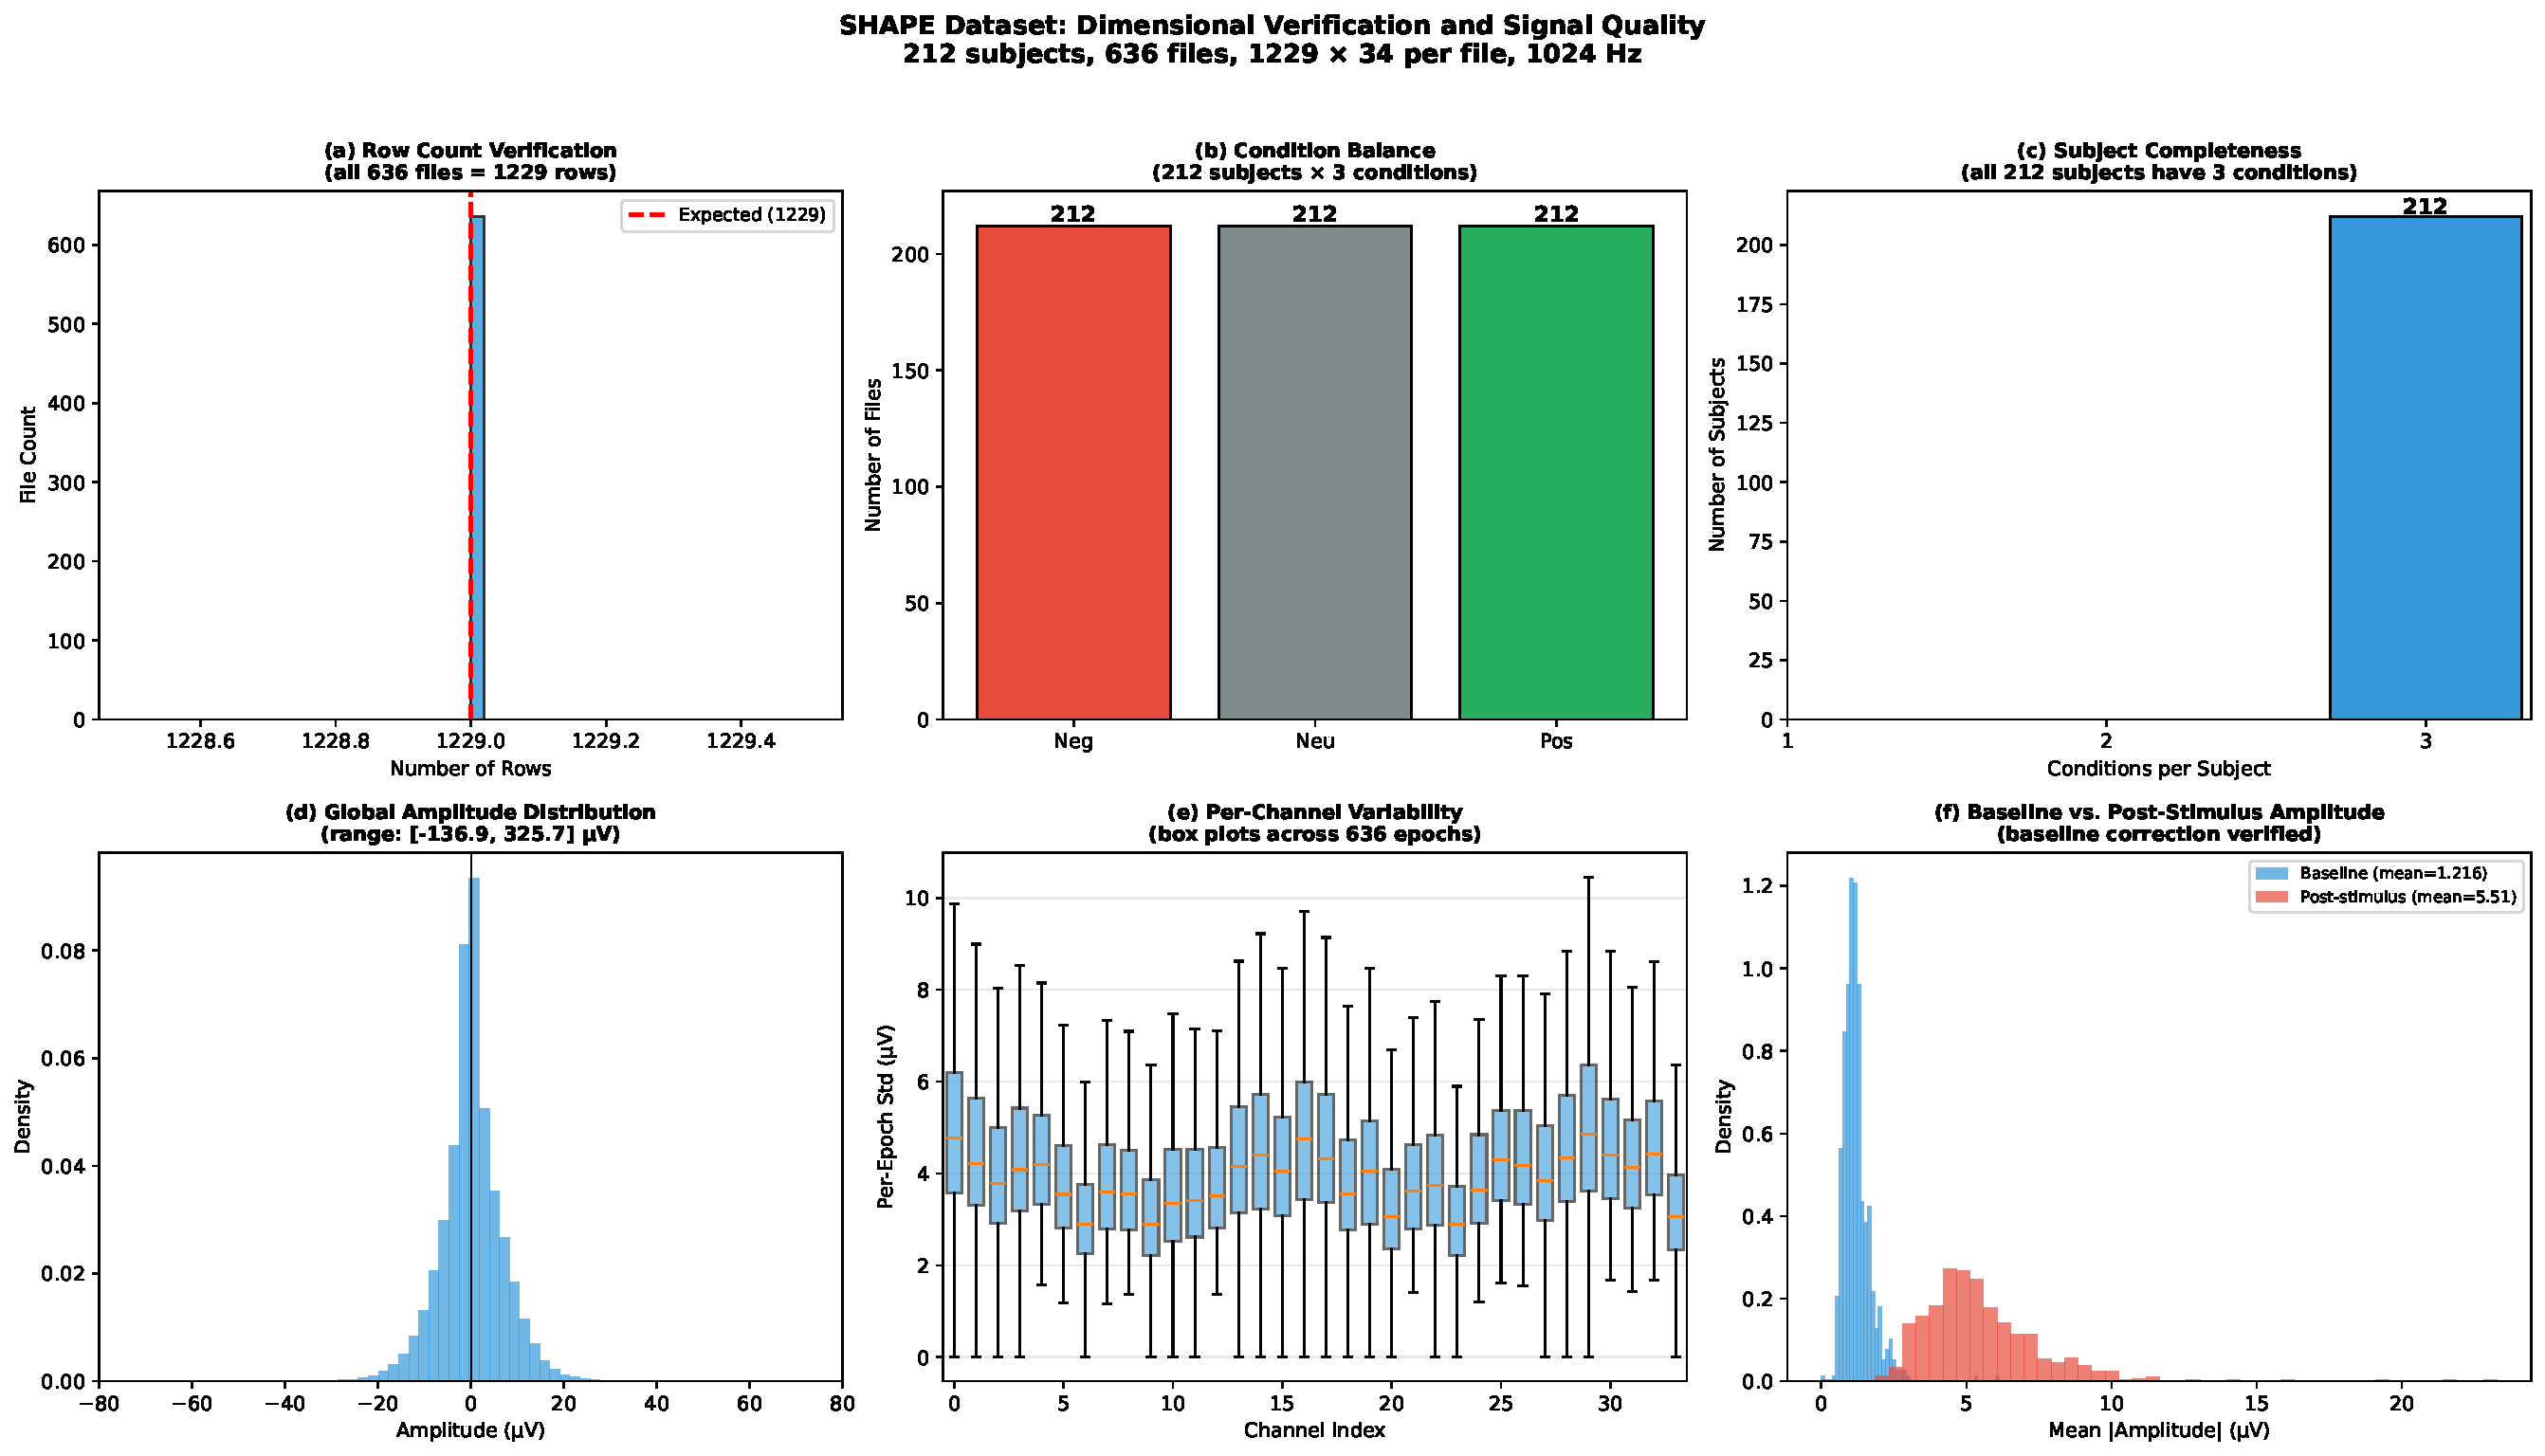
\includegraphics[width=\textwidth]{pictures/chGraphNeuralNetworks/fig_qc_dimensional_verification.pdf}
    \caption{Data verification across $636$ files. (a)~Row counts. (b)~Condition balance. (c)~Subject completeness. (d)~Global amplitude distribution. (e)~Per-channel variability. (f)~Baseline vs.\ post-stimulus amplitude.}
    \label{fig:qc_verification}
\end{figure}

\begin{figure}[H]
    \centering
    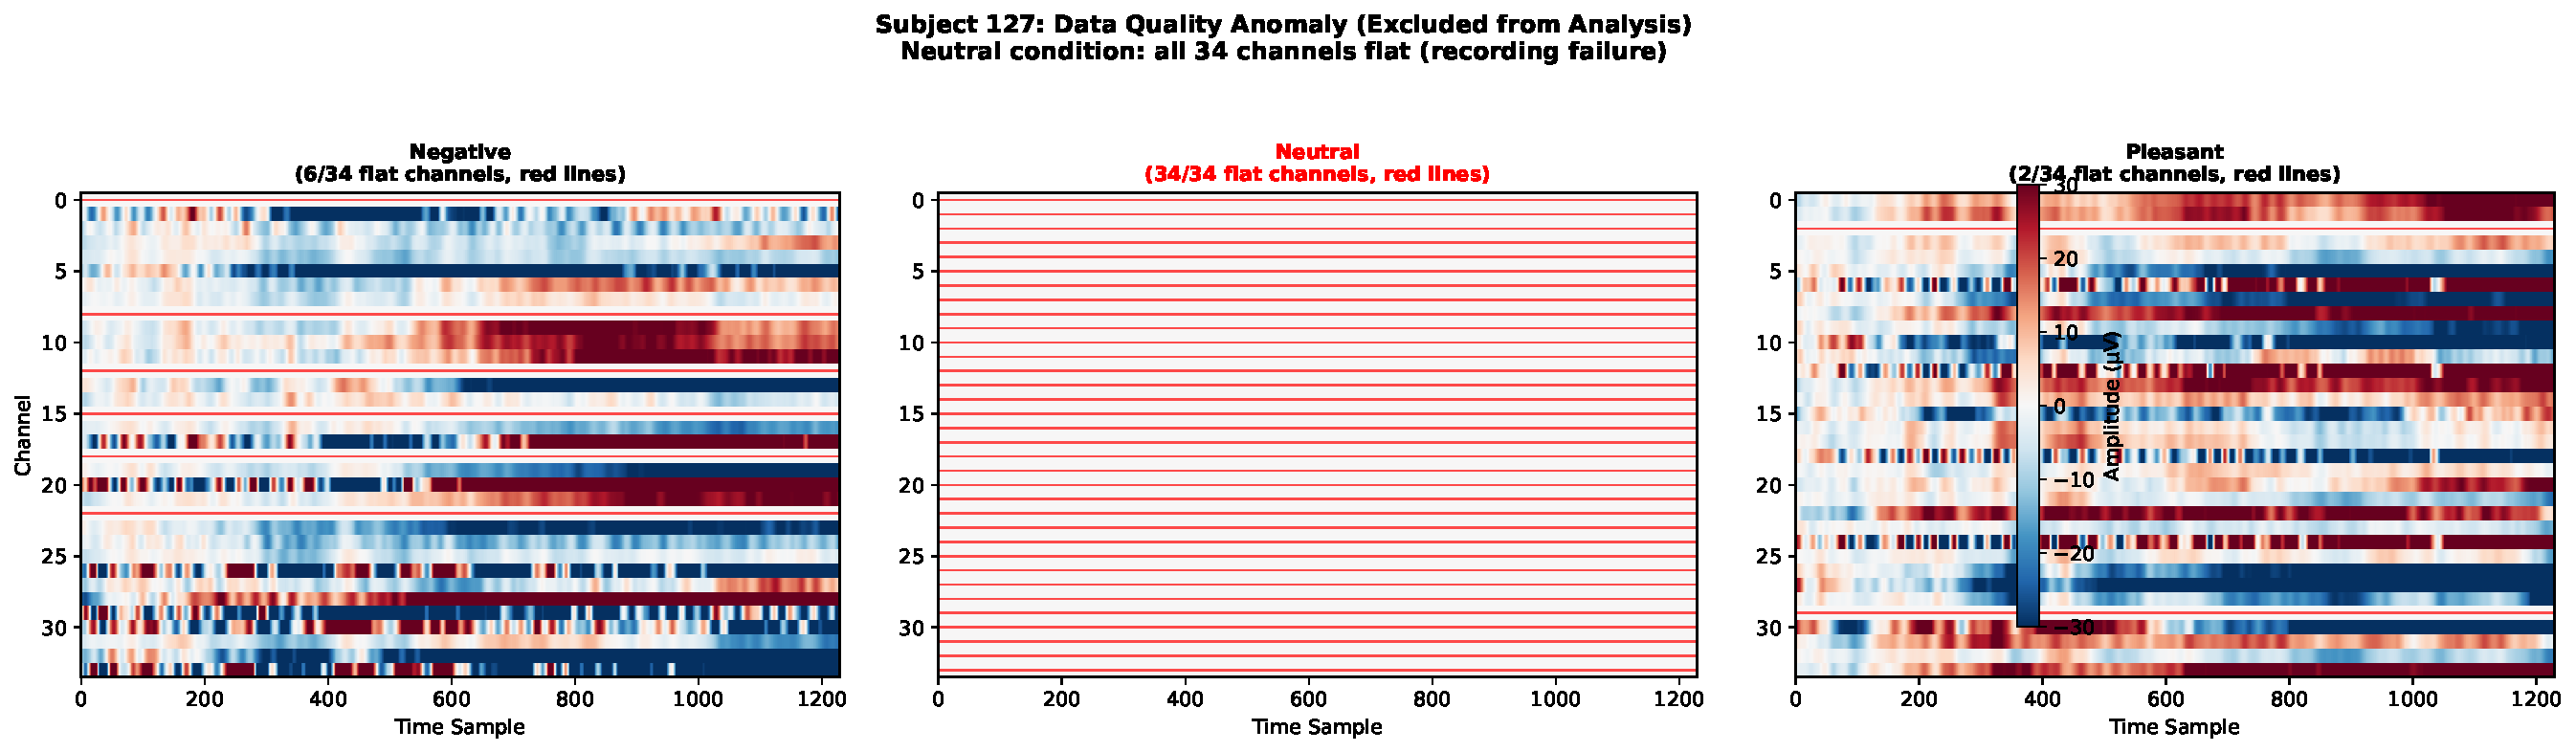
\includegraphics[width=\textwidth]{pictures/chGraphNeuralNetworks/fig_qc_subject127_anomaly.pdf}
    \caption{Subject~$127$ recording anomaly. The Neutral condition is entirely flat across all $34$ channels. Red lines indicate flat channels. This subject was excluded from all analyses.}
    \label{fig:qc_subject127}
\end{figure}

The final dataset comprises $\mathbf{211}$ \textbf{subjects} $\times$ $\mathbf{3}$ \textbf{conditions} $= \mathbf{633}$ \textbf{observations}.

\subsection{Clinical Metadata}

All $211$ subjects have comprehensive diagnostic metadata from structured clinical interviews (Figure~\ref{fig:clinical_profile}): $142$ with Major Depressive Disorder ($67.3\%$), $82$ with PTSD ($38.9\%$), $85$ with Substance Use Disorder ($40.3\%$), $60$ with GAD ($28.4\%$), $50$ with ADHD ($23.7\%$), $69$ with eating disorders ($32.7\%$), $34$ with mania ($16.1\%$), and $91$ on psychiatric medication ($43.1\%$). Biological sex: $172$ female, $33$ male. Mean comorbidity burden is $2.8$ diagnoses per subject (range $0$--$7$).

\begin{figure}[H]
    \centering
    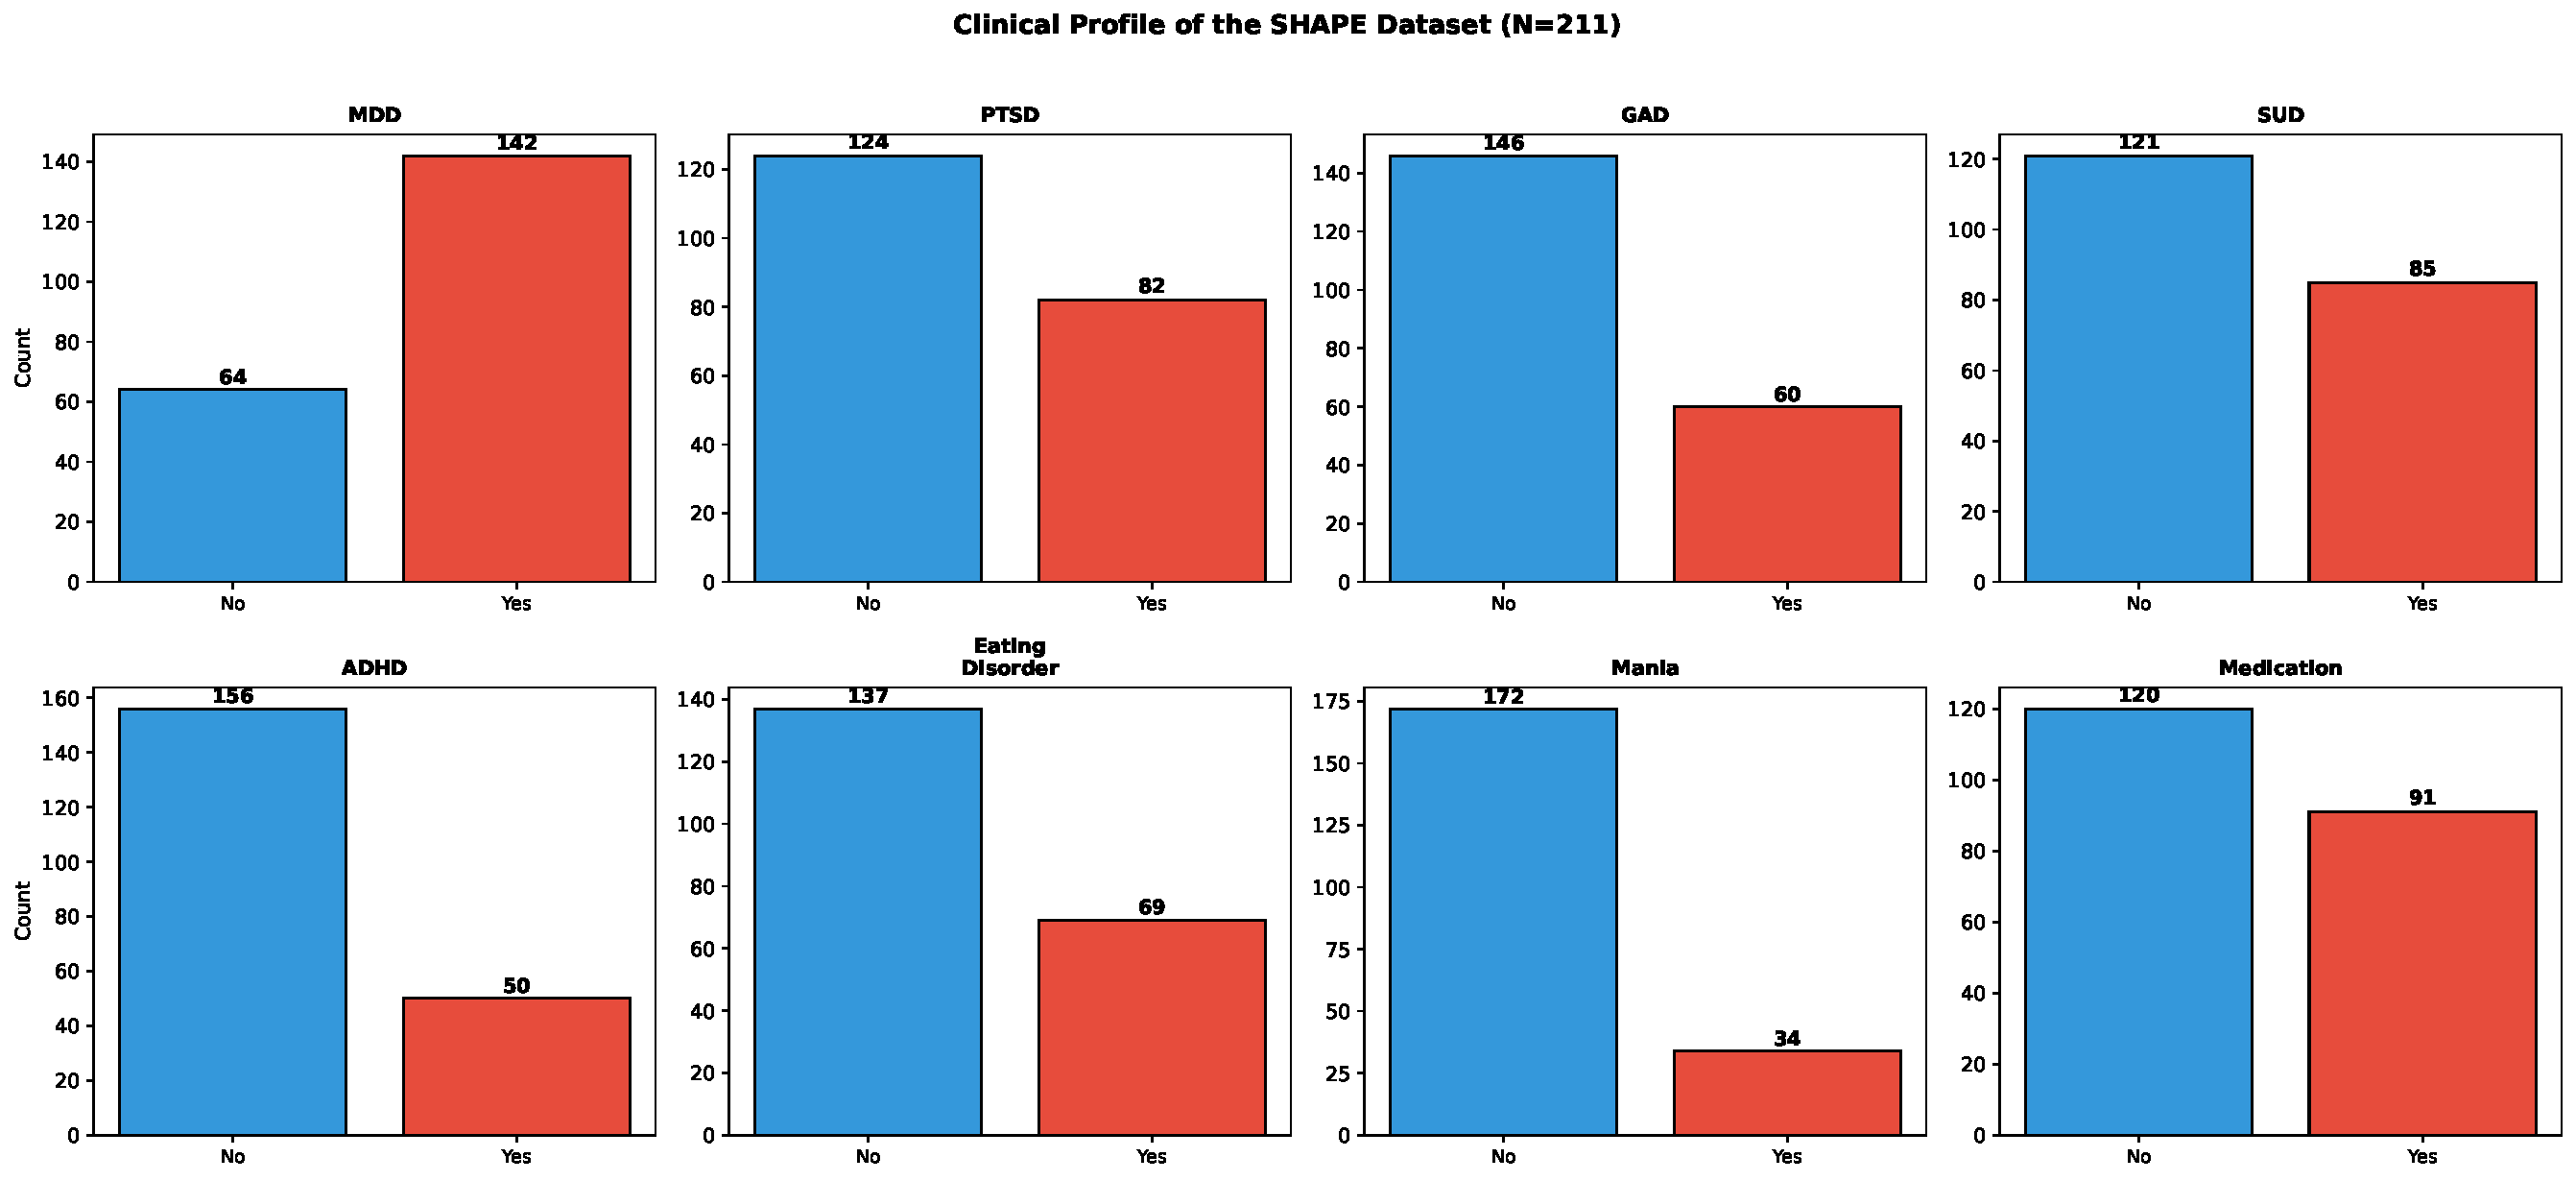
\includegraphics[width=\textwidth]{pictures/chGraphNeuralNetworks/fig_clinical_profile_211.pdf}
    \caption{Clinical profile of the $211$ SHAPE subjects. Eight diagnostic variables with group sizes.}
    \label{fig:clinical_profile}
\end{figure}

\subsection{Preprocessing Pipeline}

Four steps transform each raw $1229 \times 34$ ERP matrix into the reservoir format: baseline removal (discard first $205$ rows), $4\times$ anti-aliasing decimation to $256$~Hz ($256$ samples), per-channel z-score normalization, and LIF reservoir processing ($N_{\text{res}} = 256$, $\beta = 0.05$, $M_{\text{th}} = 0.5$) with BSC$_6$ encoding and PCA-64 reduction. The output is a $34 \times 64$ node feature matrix per observation.


\section{Raw Data Observations}
\label{sec:ch5_raw_obs}

Before classification and clinical analysis, this section characterizes the data at every stage of the graph pipeline: the z-scored multichannel EEG, the reservoir's spike response on real signals, the PCA-64 embedding geometry, the inter-channel connectivity structure, and the between-subject graph variability. These observations reveal several features of the data that constrain and inform all downstream analyses.

\subsection{Multichannel EEG Entering the Graph Stage}

The preprocessed dataset provides $633$ epochs ($211$ subjects $\times$ $3$ conditions), each a $256 \times 34$ matrix of z-scored amplitudes at $256$~Hz. Figure~\ref{fig:obs01_eeg} displays representative epochs for three subjects spanning the clinical spectrum. After per-channel z-scoring, the global distribution is centered at $0.000$ with unit variance and a range of $[-5.41, 5.01]$. Visual inspection reveals substantial inter-subject variability in waveform morphology: the temporal structure of the multichannel response differs markedly across subjects, even within the same emotional condition. This variability is the dominant signal in the data and explains why subject-level cross-validation is essential.

\begin{figure}[H]
    \centering
    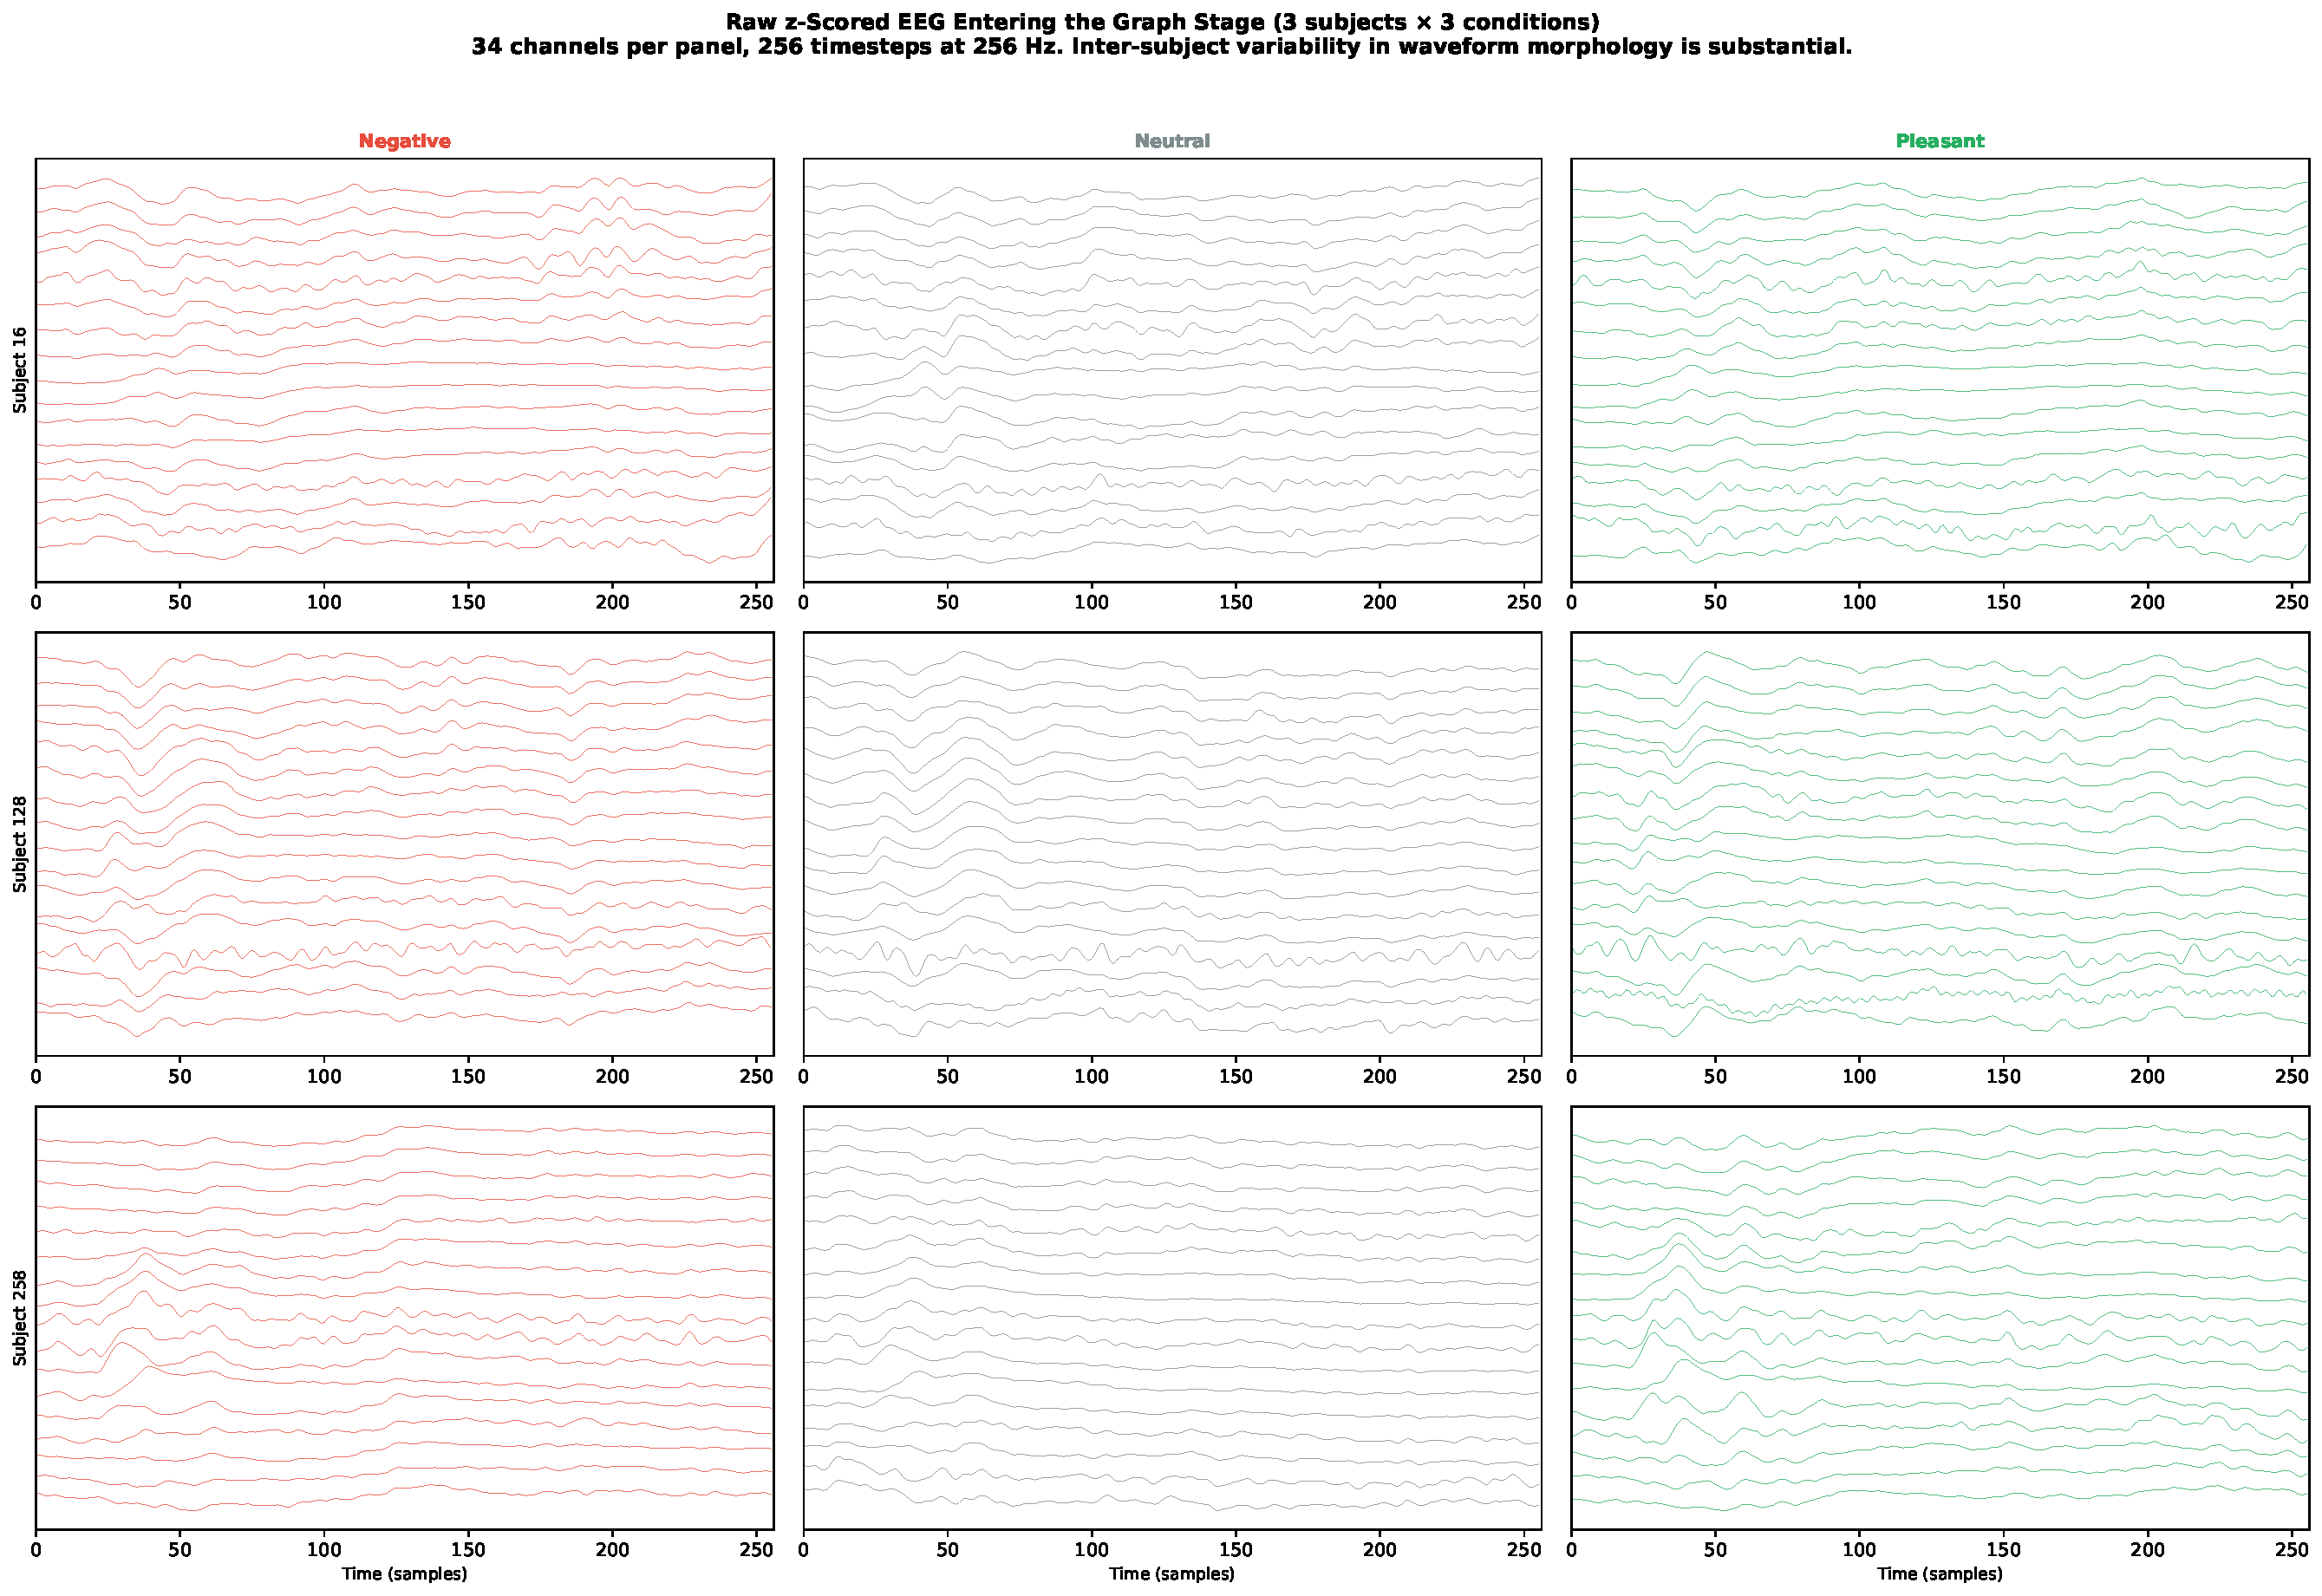
\includegraphics[width=\textwidth]{pictures/chGraphNeuralNetworks/obs01_raw_eeg_waveforms.pdf}
    \caption{Raw z-scored EEG entering the graph stage ($3$ subjects $\times$ $3$ conditions). Each panel shows $17$ of $34$ channels offset vertically, $256$ timesteps. Inter-subject waveform variability is substantially larger than between-condition differences within each subject.}
    \label{fig:obs01_eeg}
\end{figure}

\subsection{Reservoir Spike Response on Real EEG}

Figure~\ref{fig:obs02_spikes} shows the LIF reservoir's response to real SHAPE EEG for a representative subject across all three conditions. The top row displays spike rasters for a single channel (Channel~10): the reservoir transforms the continuous z-scored input into sparse binary spike trains whose temporal density tracks the input amplitude envelope. The bottom row shows population firing rate traces for four channels, revealing that different channels produce different temporal activation profiles---the inter-channel heterogeneity that the graph analysis will exploit. The BSC$_6$ features extracted from these spike trains have $47.4\%$ zero entries (compared to $79.1\%$ on the synthetic task), reflecting the richer and more sustained drive from real EEG relative to the brief synthetic pulses. Mean BSC$_6$ feature value is $5.15$ with a maximum of $42$ spikes per neuron per bin.

\begin{figure}[H]
    \centering
    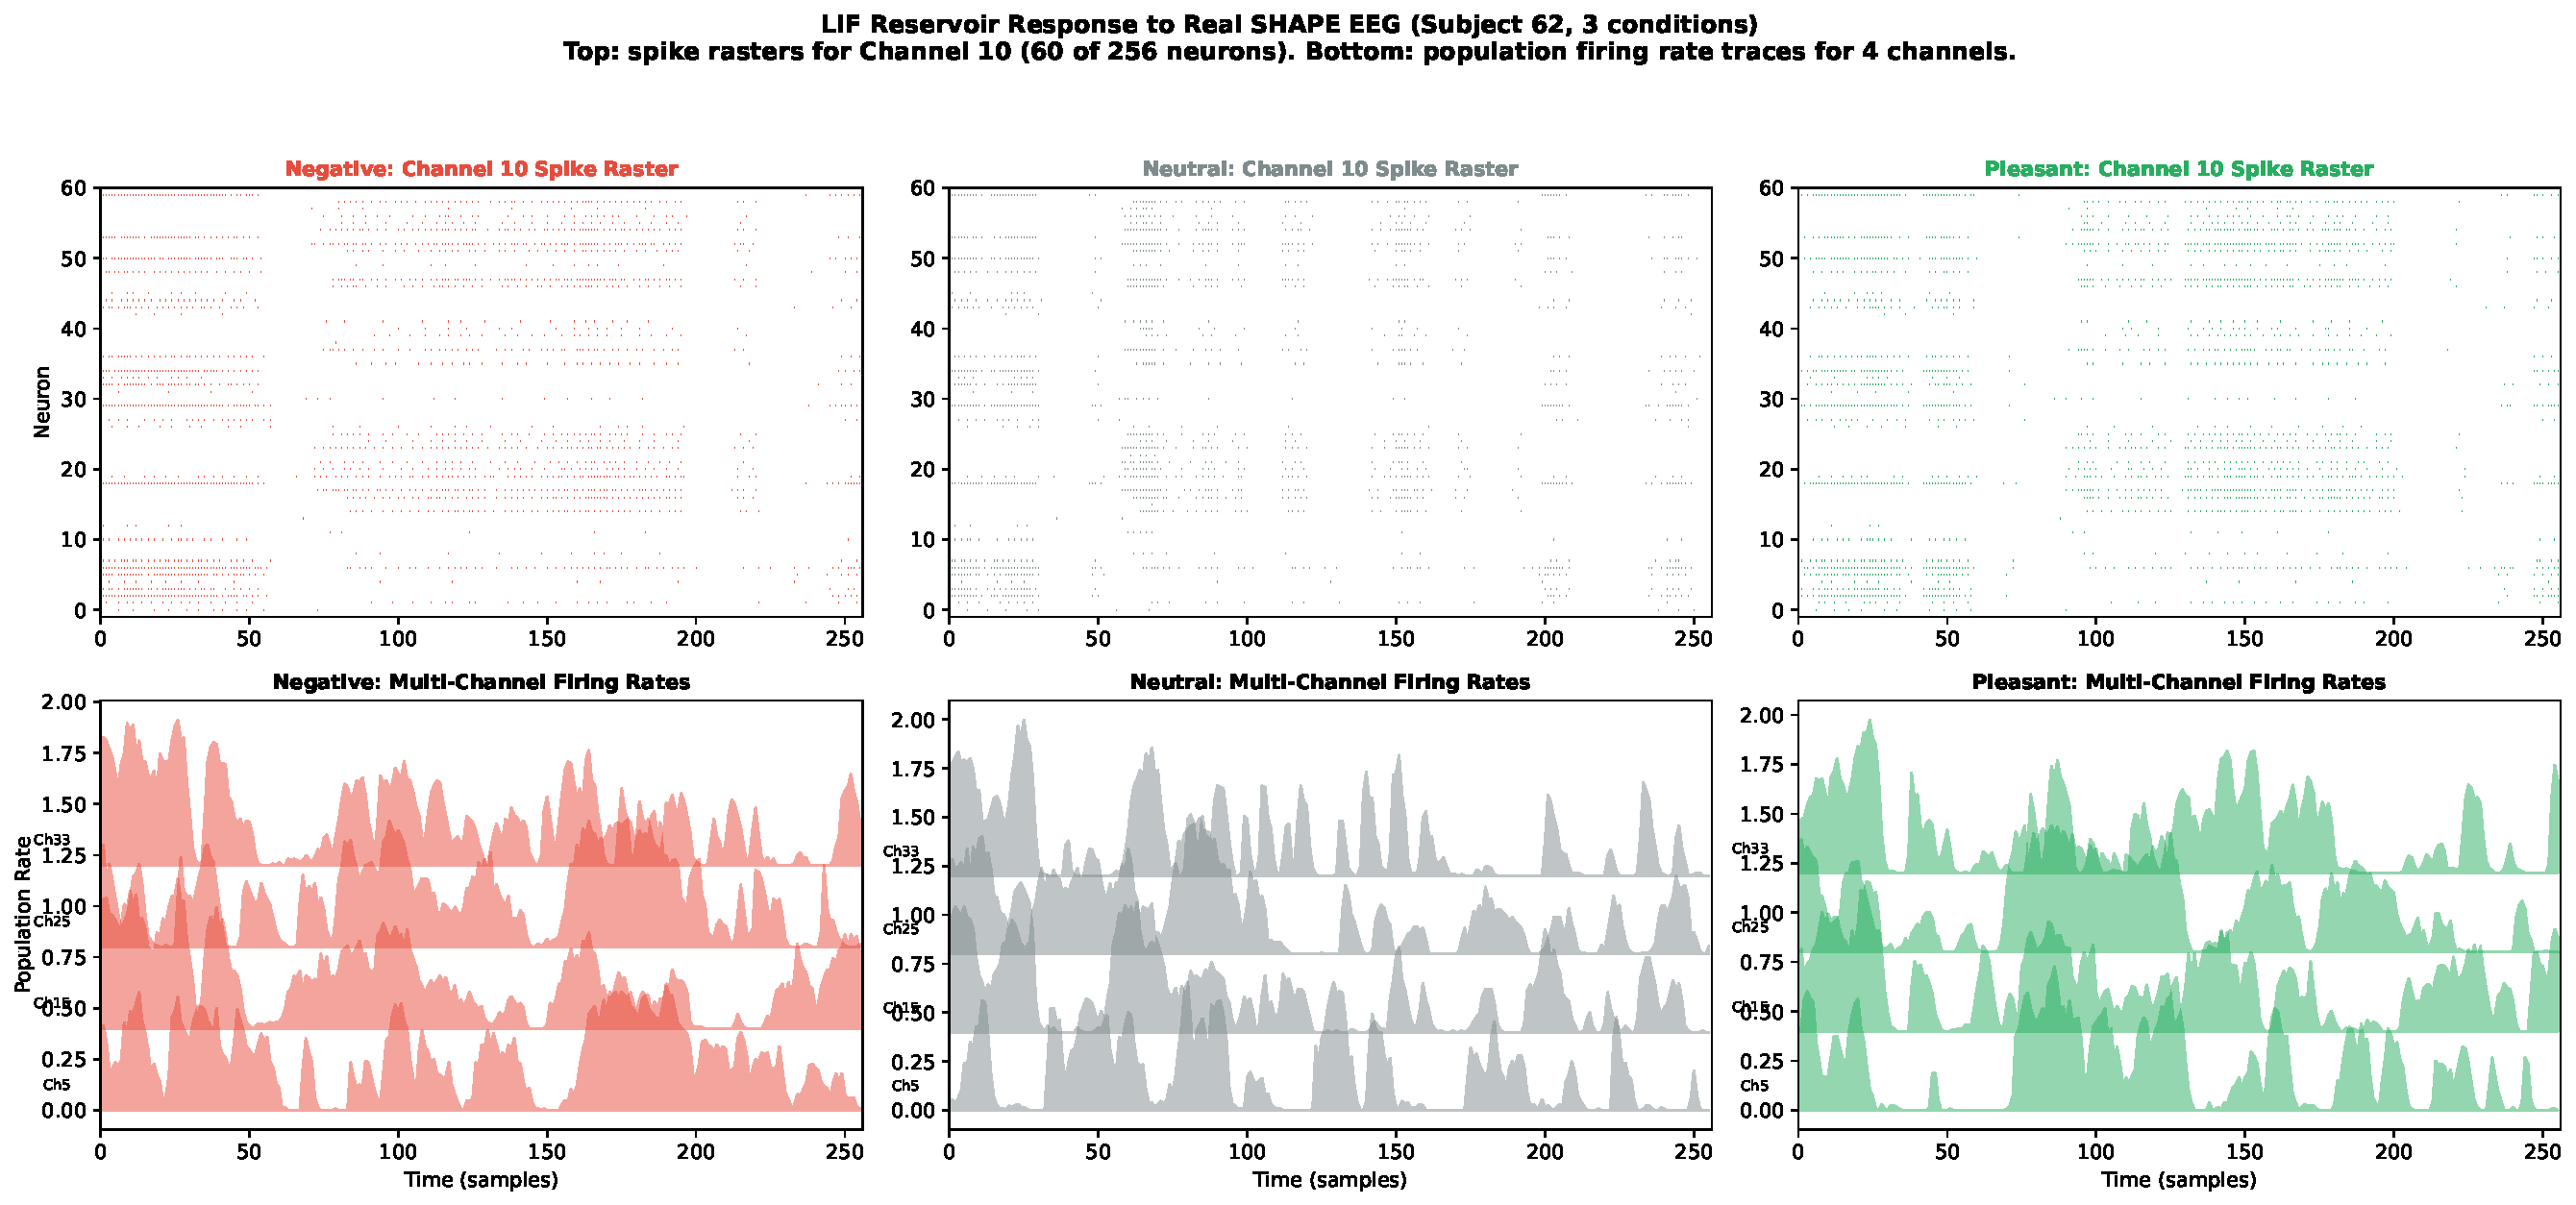
\includegraphics[width=\textwidth]{pictures/chGraphNeuralNetworks/obs02_raw_spike_trains.pdf}
    \caption{LIF reservoir response to real SHAPE EEG (one subject, three conditions). Top: spike rasters for Channel~10 ($60$ of $256$ neurons). Bottom: population firing rate traces for four channels. Different channels produce different temporal activation profiles, providing the inter-channel heterogeneity that graph analysis exploits.}
    \label{fig:obs02_spikes}
\end{figure}

\subsection{PCA-64 Embedding Geometry}

Figure~\ref{fig:obs03_embeddings} characterizes the PCA-64 embedding space. The left panel projects the concatenated $34 \times 64 = 2{,}176$-dimensional embeddings into two dimensions, colored by emotional condition. The three conditions overlap substantially---there is no clean geometric separation visible in two dimensions, consistent with the moderate classification accuracy ($63.4\%$) rather than near-perfect separation. The center panel colors the same projection by subject identity, revealing that subject-level clustering dominates: observations from the same subject cluster tightly regardless of condition. This confirms that between-subject variability ($\sigma_{\text{edge}} = 0.303$) is far larger than the condition-dependent signal ($|\Delta r| = 0.045$). The right panel shows per-channel embedding variance, which ranges from $36{,}900$ (Channel~16) to $70{,}721$ (Channel~29) with a coefficient of variation of $0.15$. This $1.9\times$ range indicates moderate heterogeneity: some channels carry more total variance than others, though all channels are active.

\begin{figure}[H]
    \centering
    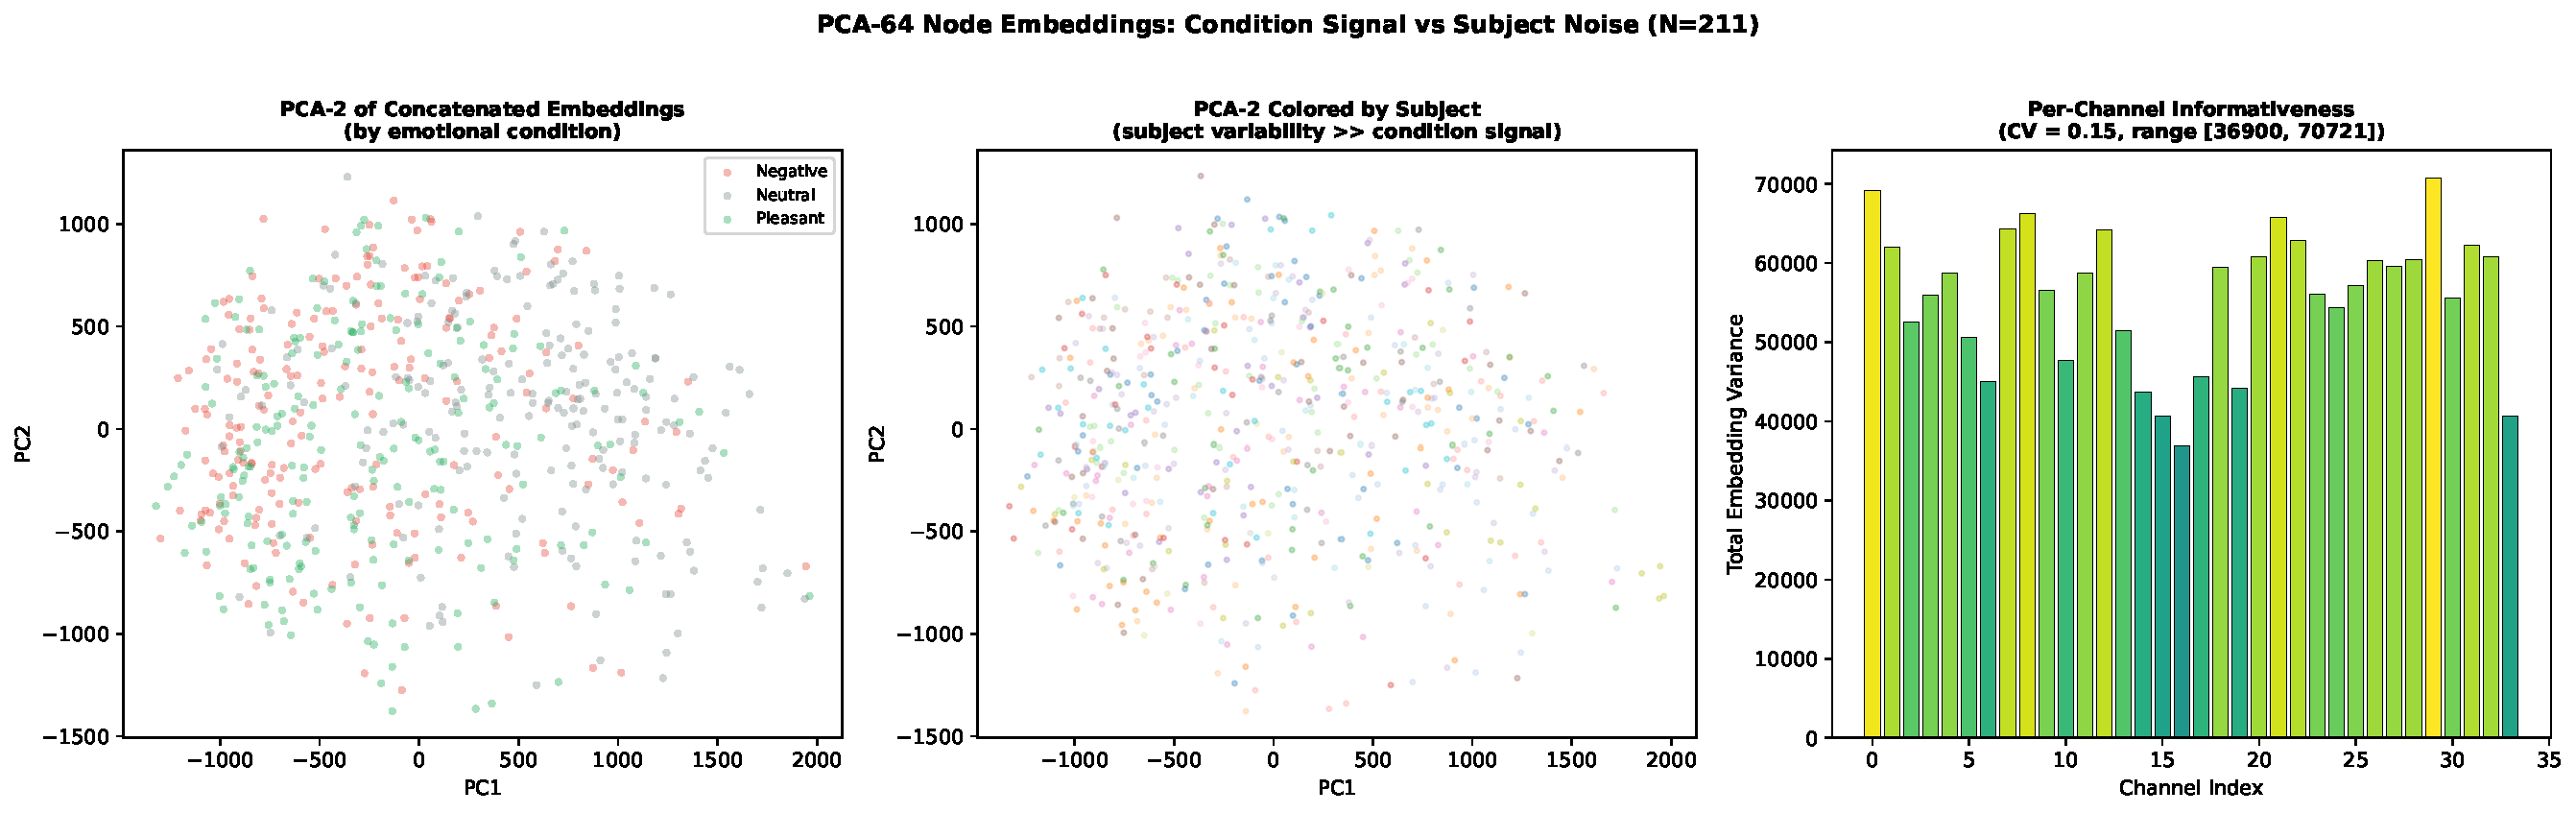
\includegraphics[width=\textwidth]{pictures/chGraphNeuralNetworks/obs03_bsc6_pca64_embeddings.pdf}
    \caption{PCA-64 embedding geometry ($N = 211$). Left: PCA-2 by condition (substantial overlap). Center: PCA-2 by subject (subject clustering dominates). Right: per-channel embedding variance (CV $= 0.15$, range $1.9\times$). Subject variability is the dominant source of variance in the embedding space.}
    \label{fig:obs03_embeddings}
\end{figure}

\subsection{Inter-Channel Connectivity and Graph Topology}

Figure~\ref{fig:obs04_connectivity} displays the inter-channel correlation matrices and their corresponding graph topologies for each condition. The mean Pearson correlation across all observations is $\bar{r} = 0.143$ with standard deviation $0.552$, indicating broad and heterogeneous inter-channel relationships: $34.8\%$ of channel pairs have correlation exceeding $0.5$, while $40.8\%$ are negative. The correlation structure is condition-dependent but the differences are subtle: mean $r$ is $0.147$, $0.145$, and $0.138$ for Negative, Neutral, and Pleasant respectively.

At the $20\%$ density threshold, each condition-average graph contains $113$ edges with mean degree $6.6$ and maximum degree $13$. The graphs (Figure~\ref{fig:obs04_connectivity}, bottom row) show that the topology is not uniform: some channels are hubs (degree $> 10$) while others are peripheral (degree $= 1$--$2$). The mean clustering coefficient is $0.804$, indicating high local redundancy---neighbors of a node tend to be neighbors of each other. The thresholded correlation values range from $r = 0.506$ (Pleasant) to $r = 0.545$ (Negative), meaning only strongly correlated pairs are retained as edges.

\begin{figure}[H]
    \centering
    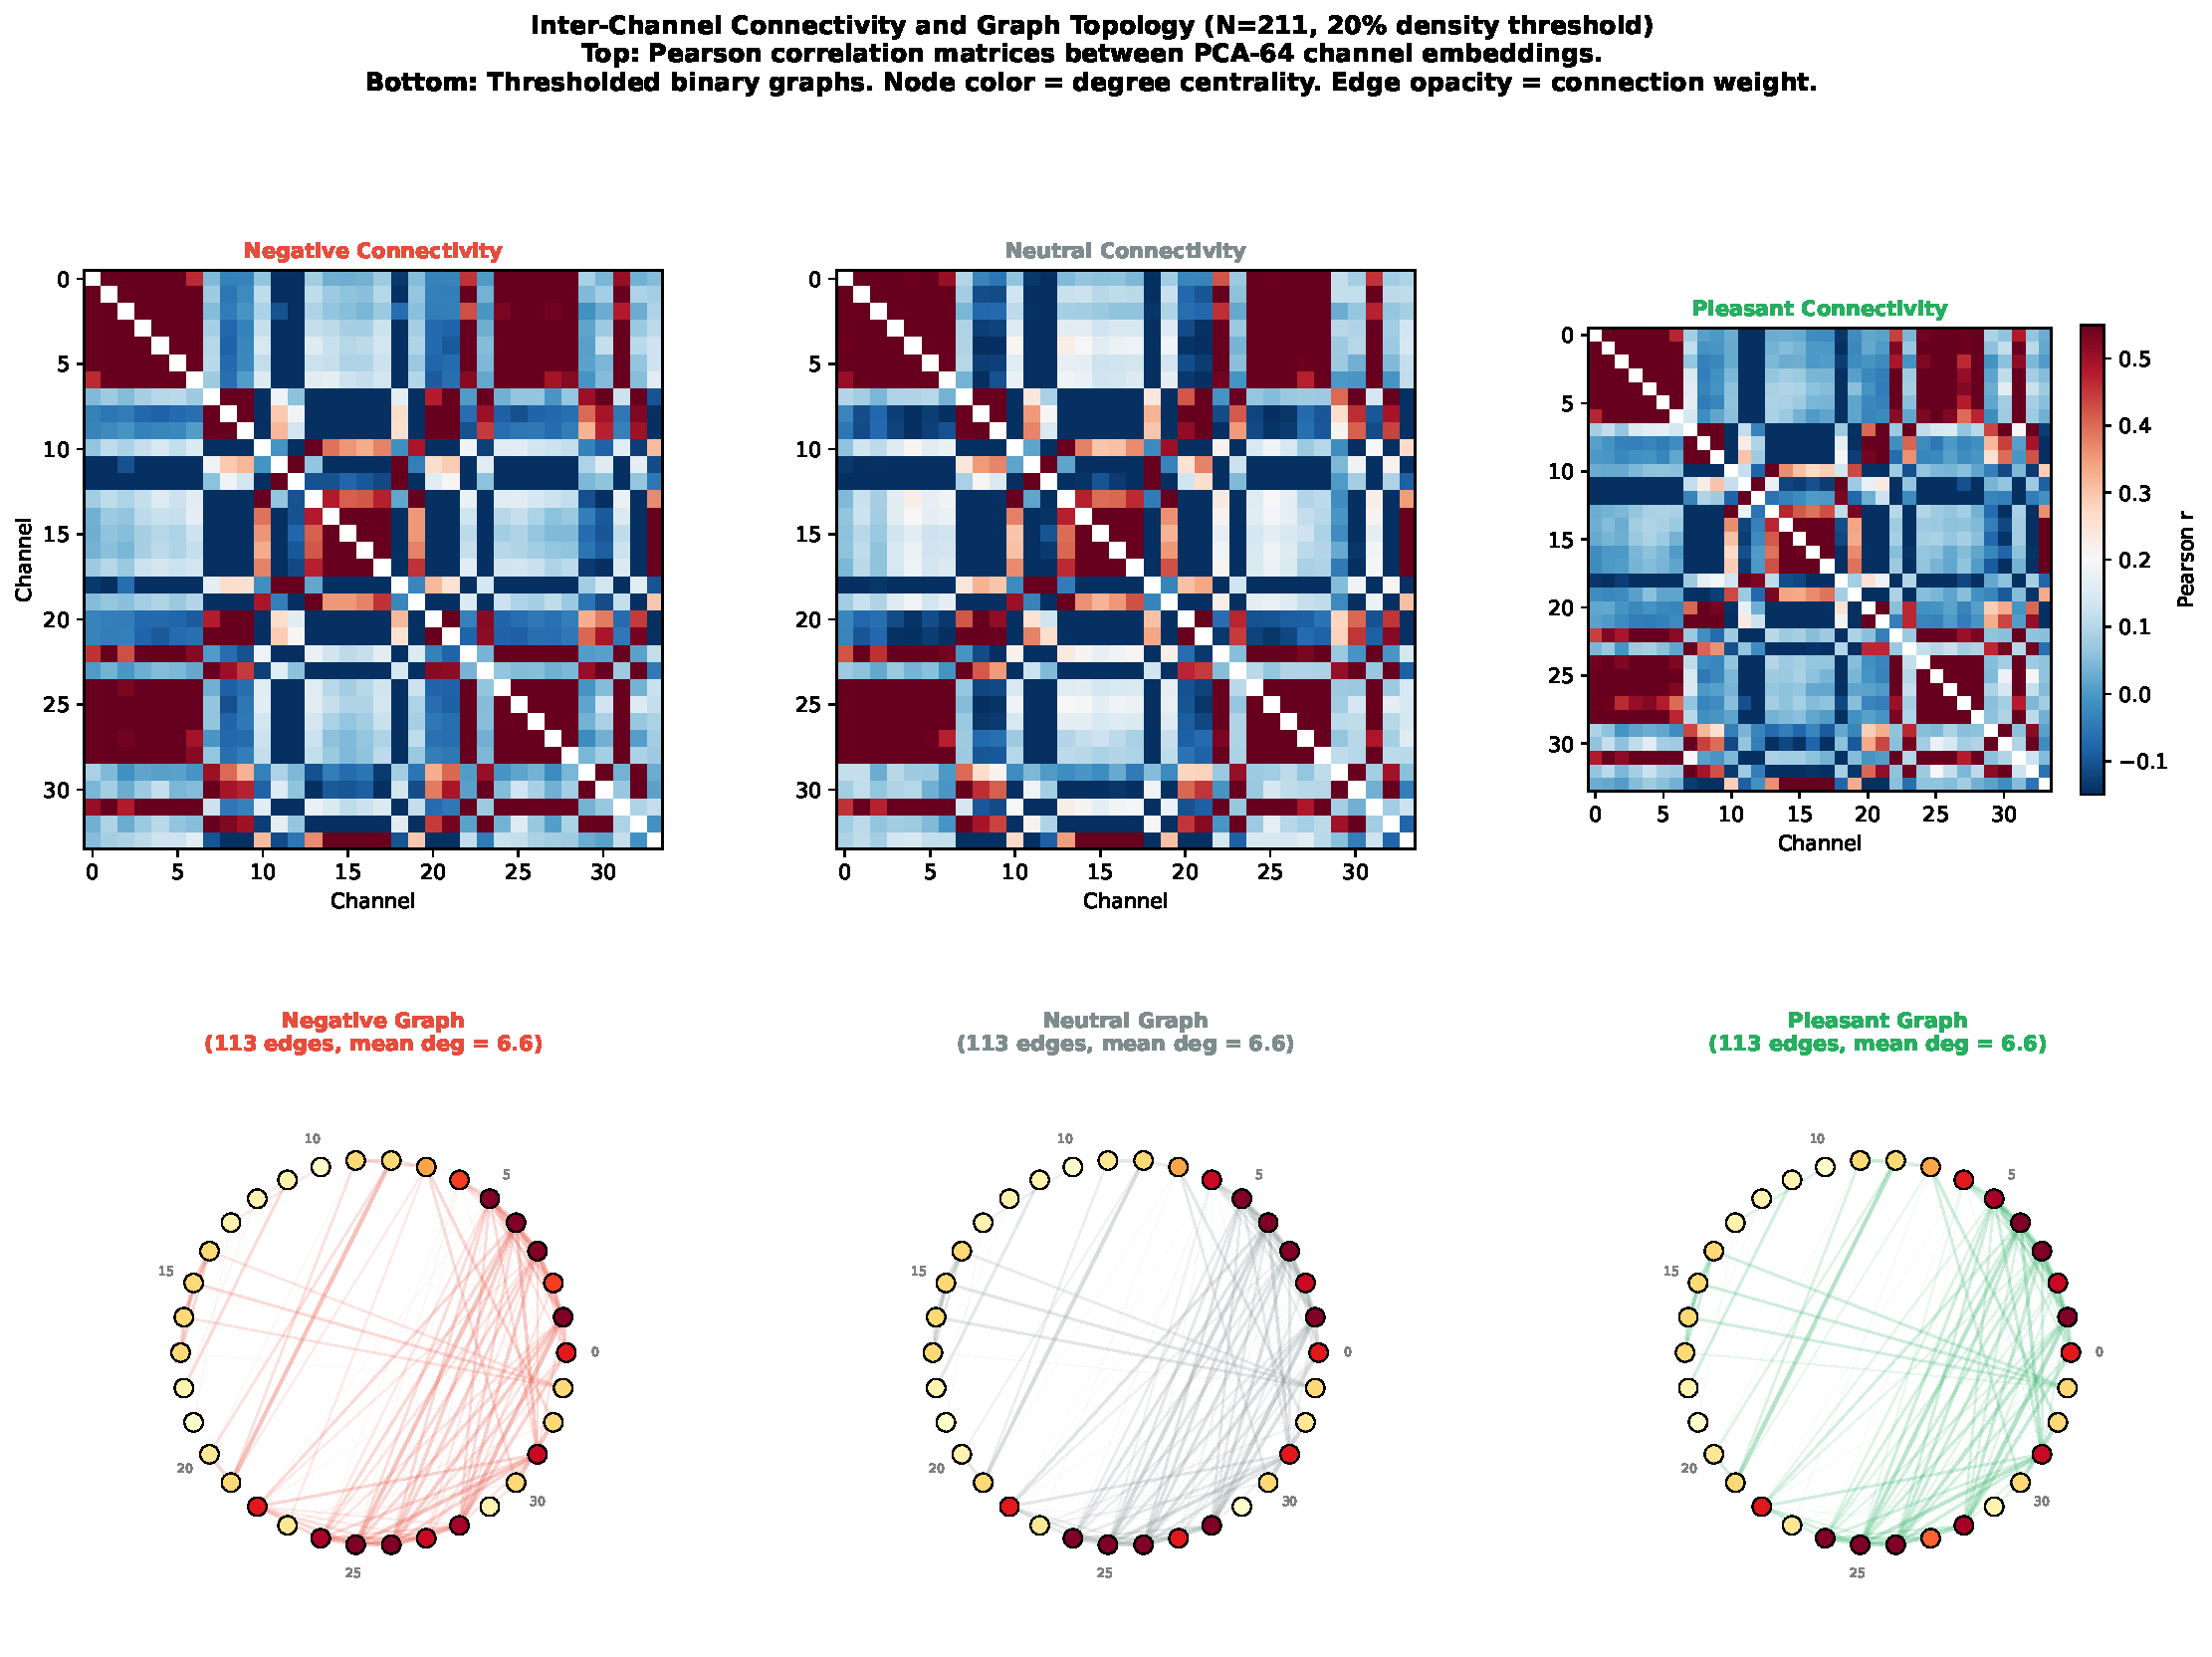
\includegraphics[width=\textwidth]{pictures/chGraphNeuralNetworks/obs04_raw_connectivity_matrices.pdf}
    \caption{Inter-channel connectivity and graph topology ($N = 211$, $20\%$ density). Top: Pearson correlation matrices (mean $\bar{r} = 0.143$, $34.8\%$ of pairs $> 0.5$, $40.8\%$ negative). Bottom: thresholded graphs with $113$ edges each. Node color $=$ degree centrality; edge opacity $\propto$ connection weight. Hub and peripheral channels are visible.}
    \label{fig:obs04_connectivity}
\end{figure}

\subsection{Between-Subject Graph Variability}

Figure~\ref{fig:obs07_variability} quantifies the between-subject variability in graph structure. Individual subject graphs (top row) show substantial topological diversity: the same $20\%$ density threshold produces different hub locations, different edge patterns, and different degree distributions across subjects. The bottom-left panel shows that edge-level variability ($\sigma = 0.303$) spans the full range of edge weights, with stronger edges being more variable. The degree distribution across all subjects and channels (bottom center) is unimodal with a mean of $6.6$ and a range from $0$ to $15$.

The condition-difference graph (bottom right, Negative minus Pleasant) reveals which channel pairs show the largest emotional modulation. The signal-to-noise comparison (far right) quantifies the fundamental challenge: between-subject edge variability ($\sigma = 0.303$) is $7\times$ larger than the mean condition-dependent signal ($|\Delta r| = 0.045$). This ratio constrains every analysis in this chapter: the condition signal is real but weak relative to the dominant source of variance, which is inter-individual differences in brain network organization. Any classification or clinical analysis method must extract this weak signal from within strong subject-level noise.

\begin{figure}[H]
    \centering
    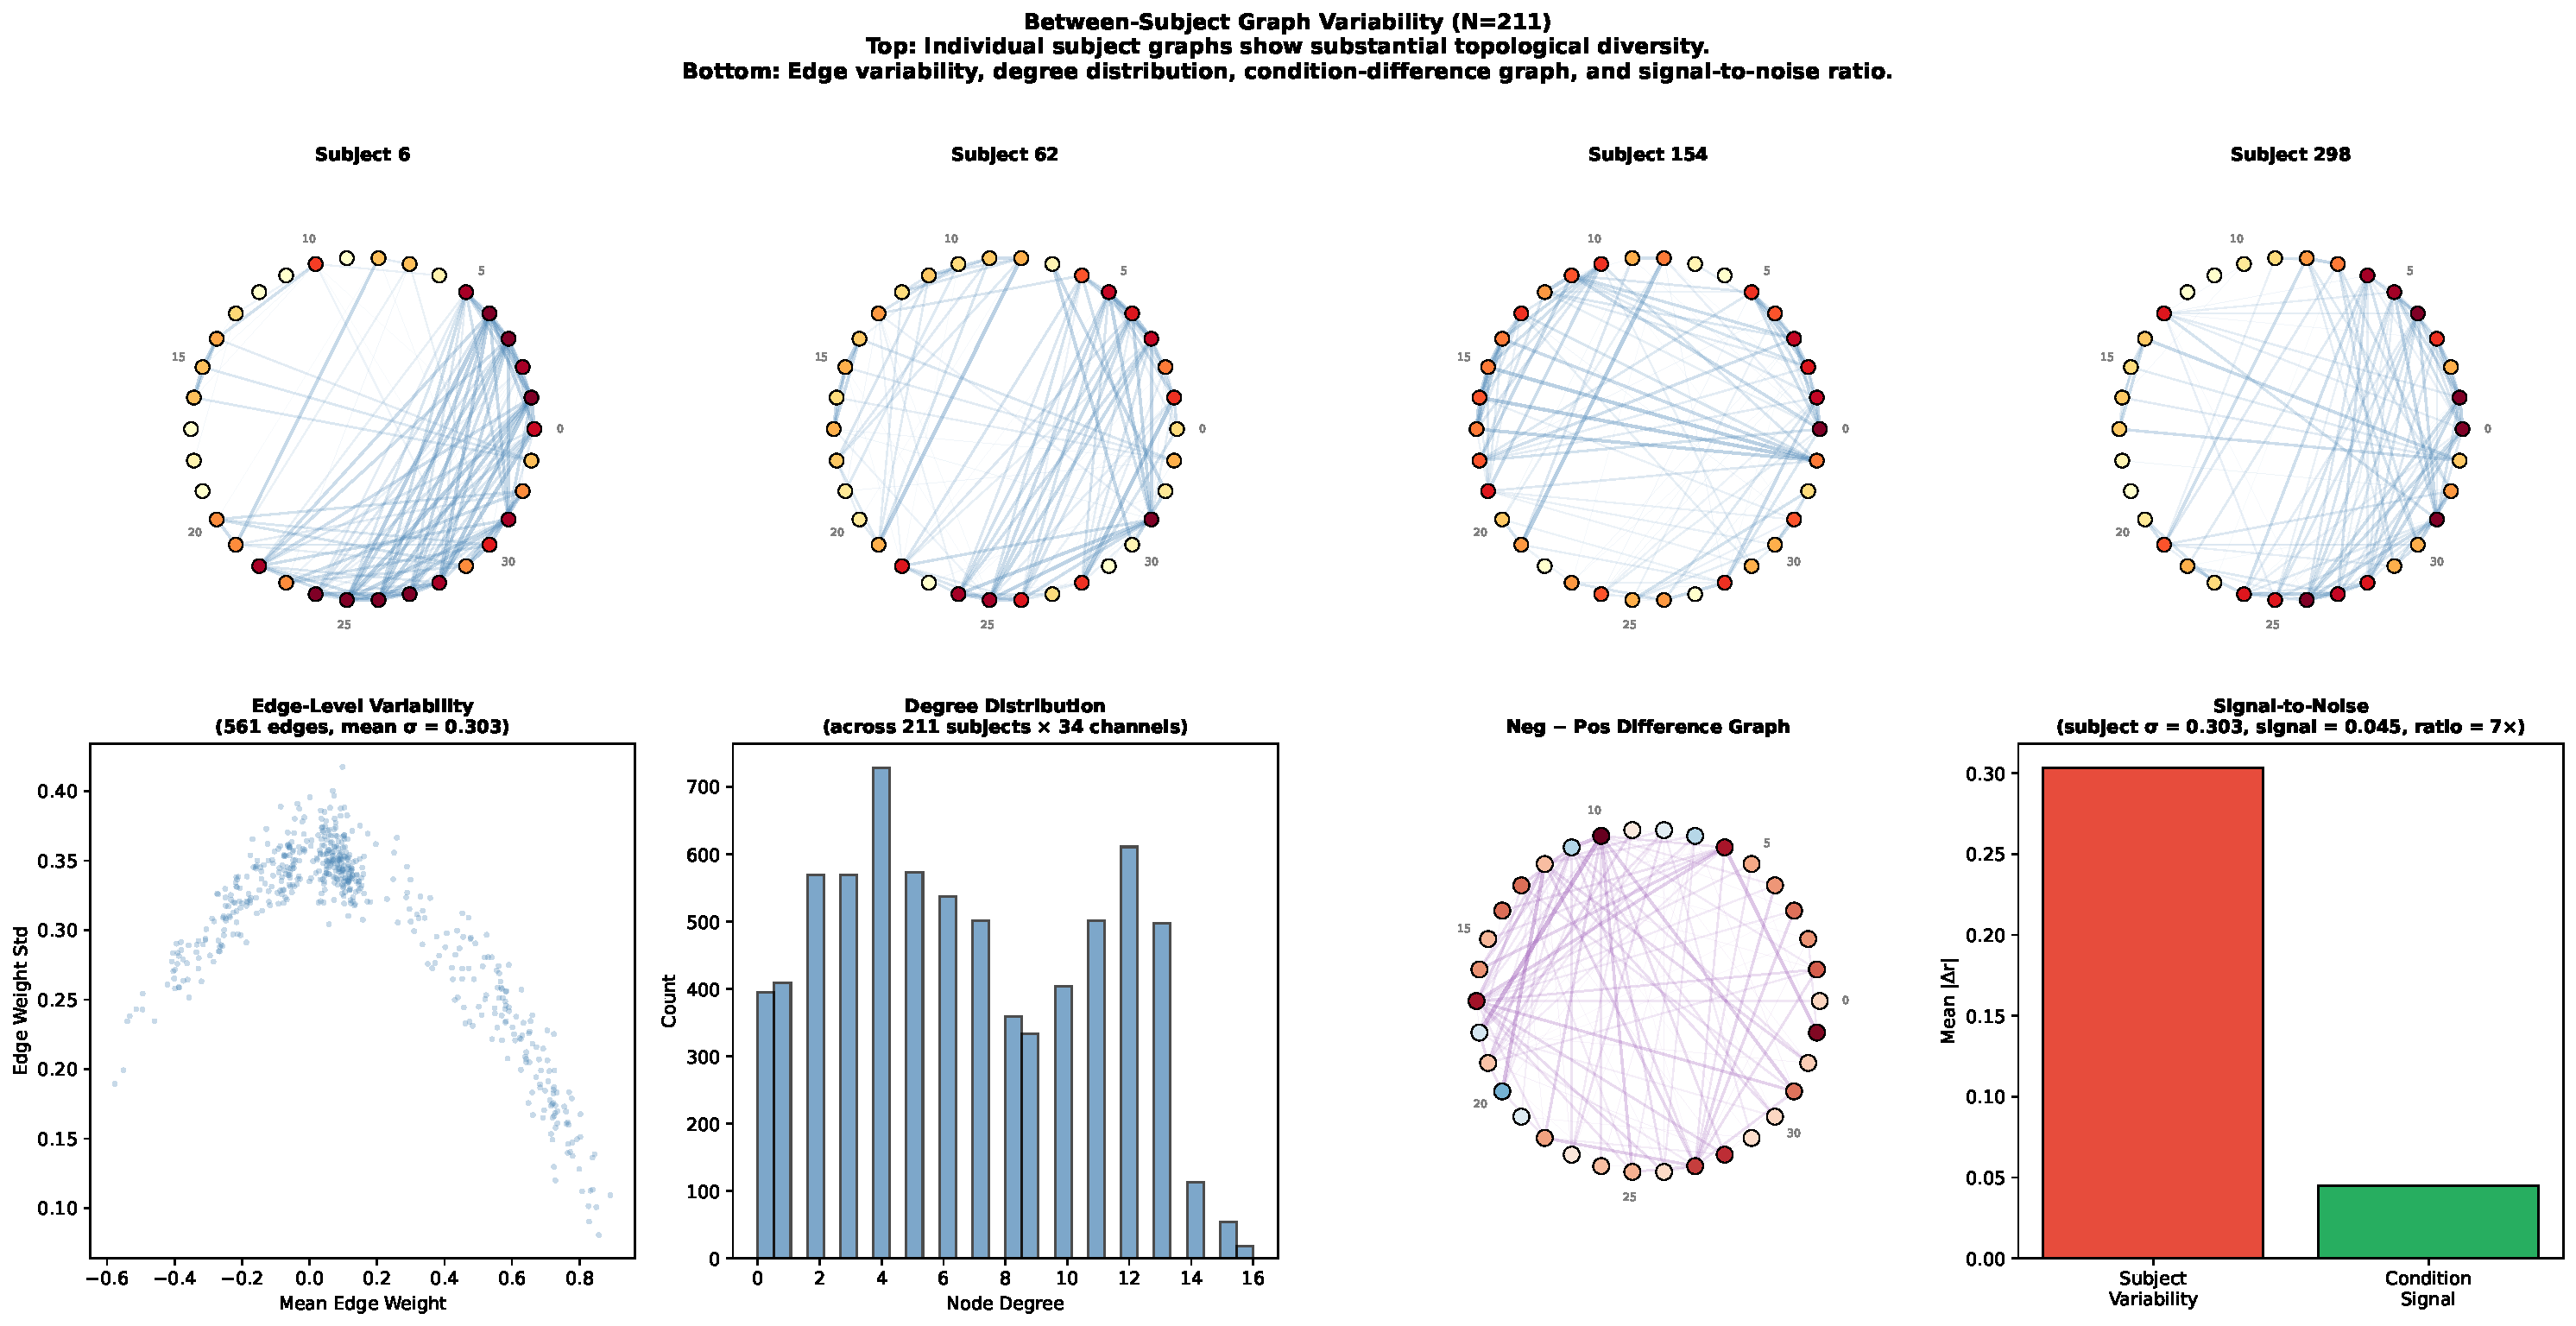
\includegraphics[width=\textwidth]{pictures/chGraphNeuralNetworks/obs07_graph_variability.pdf}
    \caption{Between-subject graph variability ($N = 211$). Top: four individual subject graphs showing topological diversity. Bottom: edge-level variability scatter ($\sigma = 0.303$), degree distribution across all subjects, condition-difference graph (Neg $-$ Pos), and signal-to-noise comparison ($7\times$ more subject noise than condition signal).}
    \label{fig:obs07_variability}
\end{figure}

These five observation subsections, with their associated figures and quantitative statistics, establish the data landscape. The key structural features are: (1)~subject variability dominates condition signal by $7\times$; (2)~the graph is small ($34$ nodes), dense ($20\%$, $113$ edges), and highly clustered ($\bar{C} = 0.804$); (3)~the embedding space shows moderate channel heterogeneity but no clean geometric separation by condition; and (4)~the correlation structure is broad, with $40.8\%$ negative pairs indicating genuine heterophily.

\subsection{The Reservoir's Spike Representation on Real EEG}

Figure~\ref{fig:obs13_bsc6} characterizes the BSC$_6$ feature structure that the reservoir produces from real clinical EEG---the representation that every subsequent analysis in this chapter operates on. Each observation is a $34 \times 256 \times 6$ tensor ($34$ channels, $256$ reservoir neurons, $6$ temporal bins), yielding $52{,}224$ spike-count features per observation. The representation is $47.4\%$ sparse (compared to $79.1\%$ on the synthetic task in Chapter~\ref{chap:embeddings}), reflecting the richer and more sustained drive from real EEG. Non-zero entries have a mean of $9.79$ and a median of $7$ spikes per neuron per bin, with a maximum of $42$.

\begin{figure}[H]
    \centering
    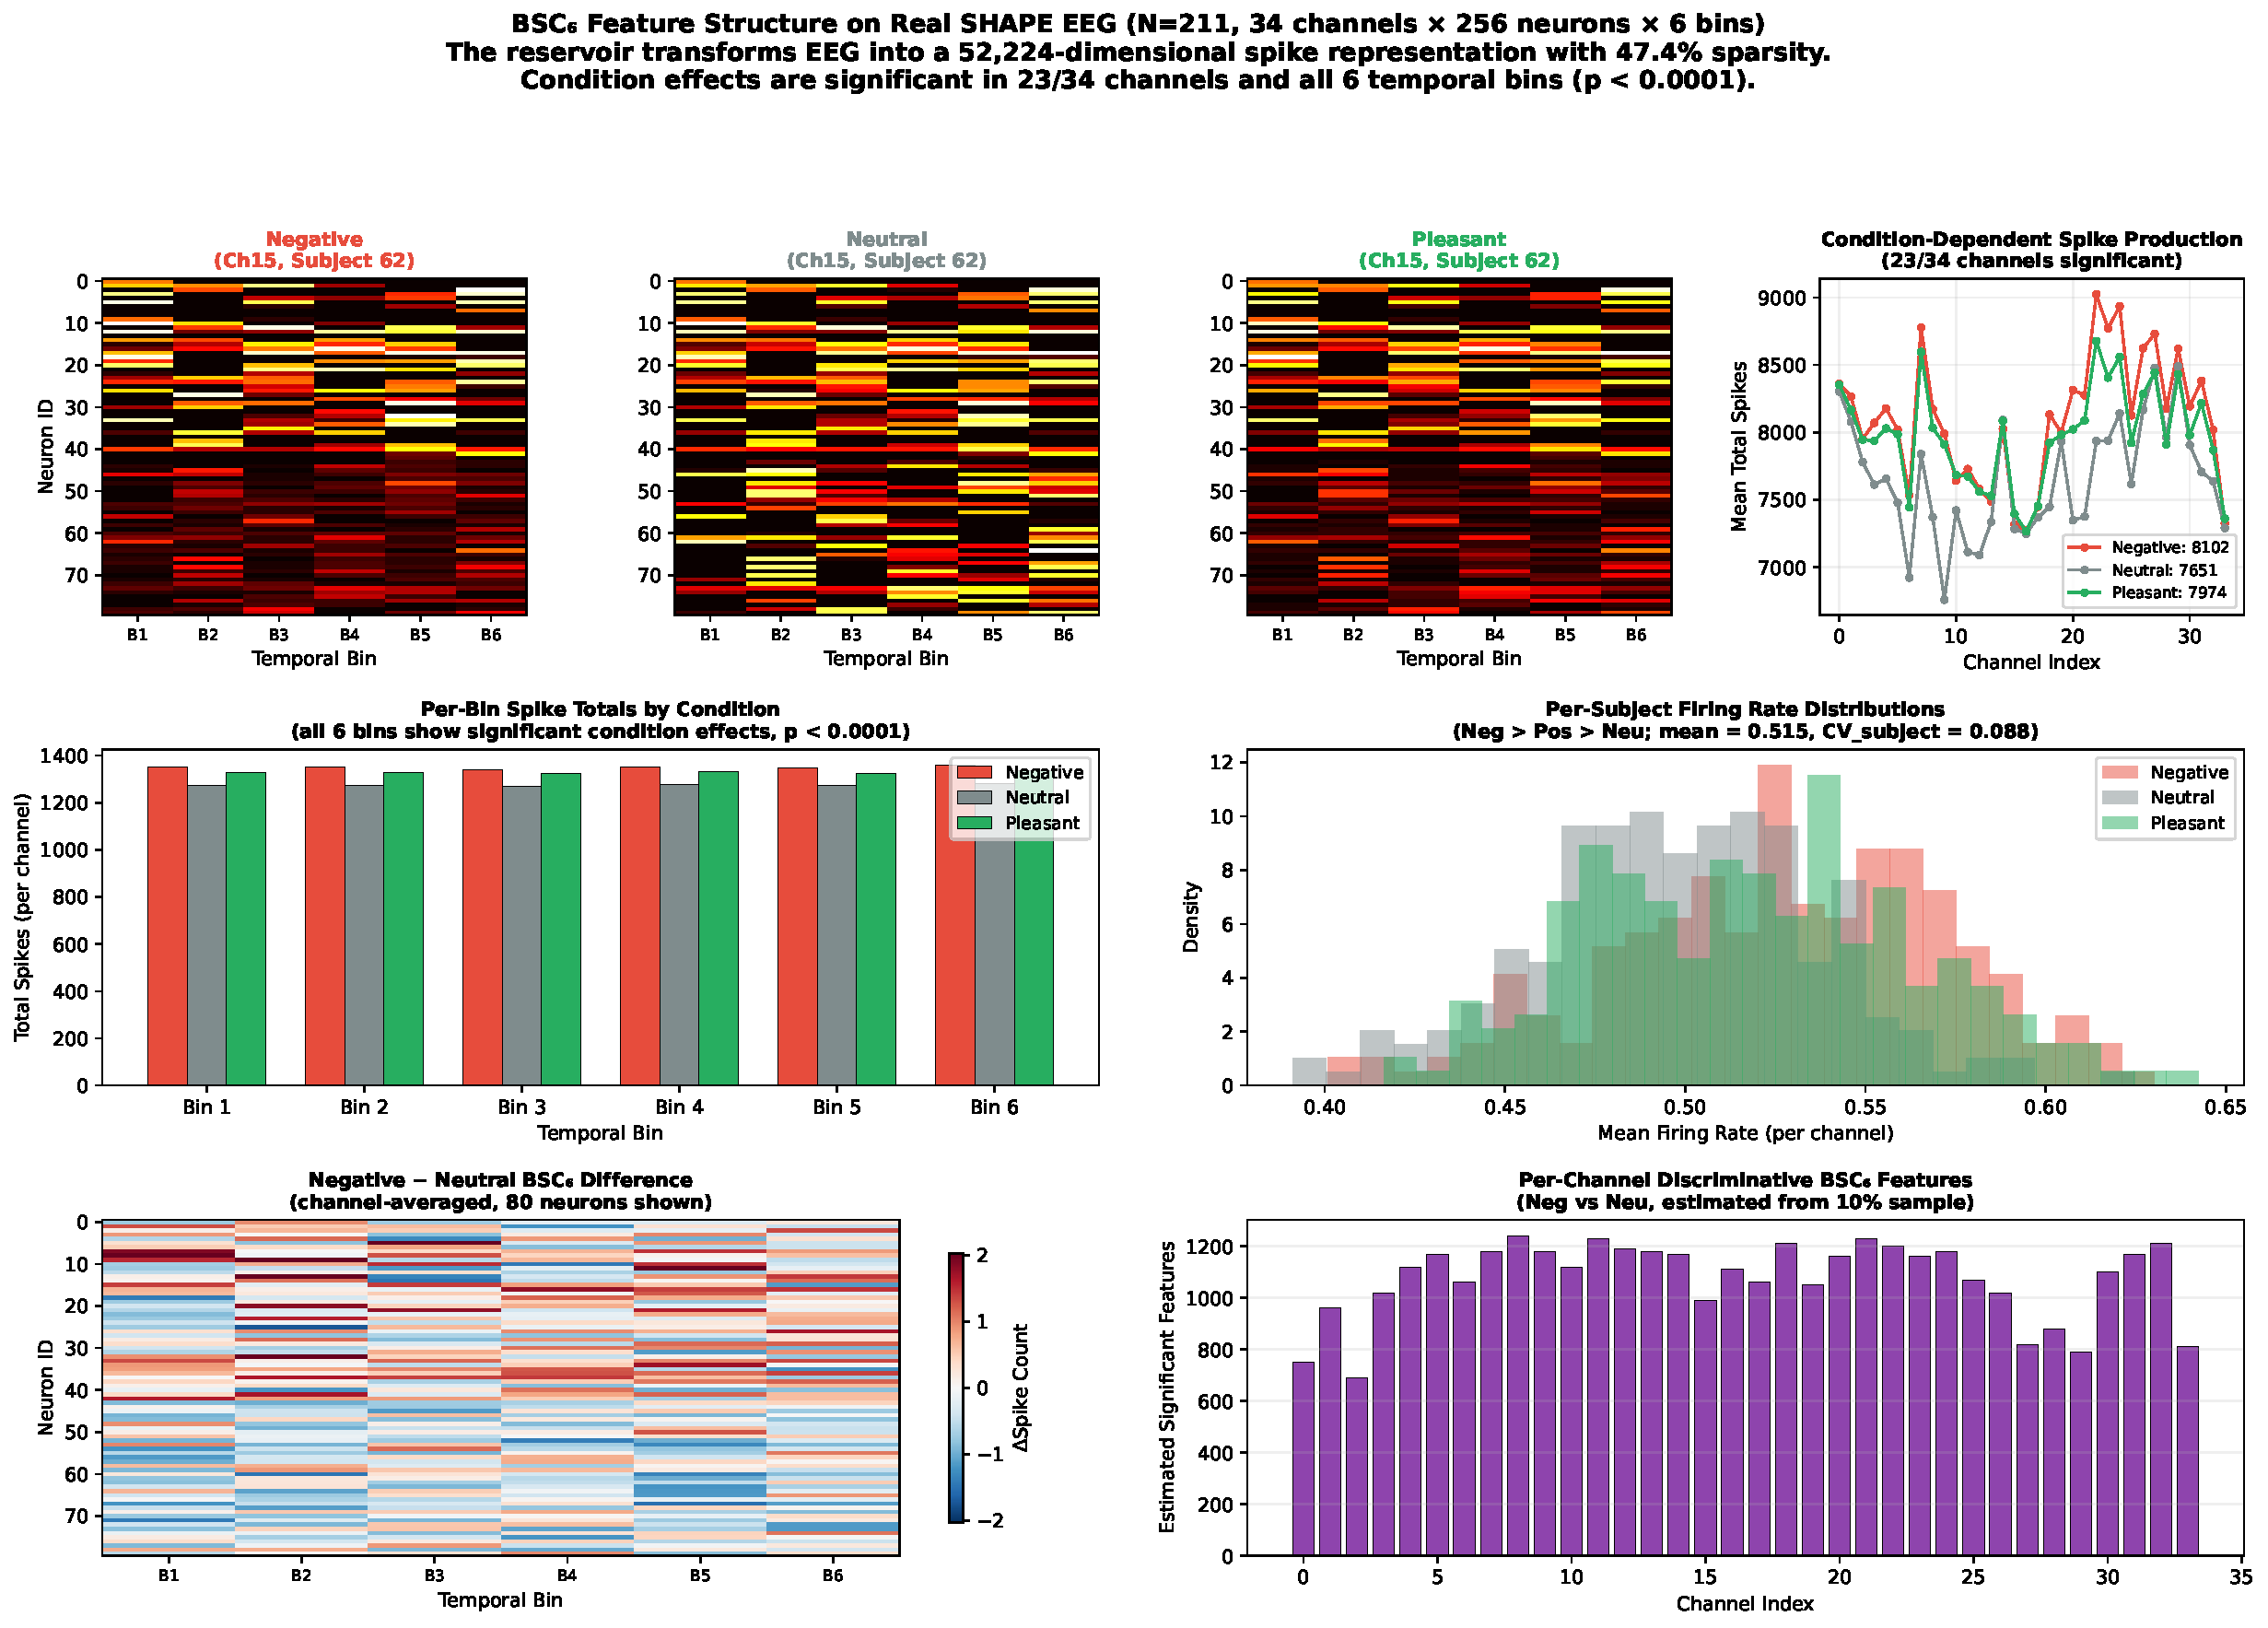
\includegraphics[width=\textwidth]{pictures/chGraphNeuralNetworks/obs13_bsc6_real_eeg.pdf}
    \caption{BSC$_6$ features on real SHAPE EEG ($N = 211$, $34$ channels $\times$ $256$ neurons $\times$ $6$ bins $= 52{,}224$ features per observation). Top: single-subject BSC$_6$ heatmaps by condition and condition-dependent spike production across channels ($23/34$ significant). Middle: per-bin spike totals by condition (all $6$ bins $p < 0.0001$) and per-subject firing rate distributions. Bottom: class-average difference map and per-channel discriminative feature counts.}
    \label{fig:obs13_bsc6}
\end{figure}

The condition structure in the spike representation is both distributed and highly significant. The Negative condition produces $8{,}102 \pm 1{,}220$ total spikes per channel, compared to $7{,}651 \pm 1{,}153$ for Neutral and $7{,}974 \pm 1{,}175$ for Pleasant. This $5.9\%$ elevation in spike production during negative emotional processing is consistent with the late positive potential (LPP) enhancement observed in the ERP literature---the reservoir's nonlinear transformation translates increased ERP amplitude into increased firing. The condition effect is significant in $23$ of $34$ channels and in \emph{all six temporal bins} ($p < 0.0001$ for every bin in the Negative--Neutral comparison). The ubiquity of this effect---distributed across neurons, channels, and temporal bins simultaneously---indicates that the reservoir encodes the emotional condition signal in a high-dimensional, distributed representation rather than concentrating it in a few features.

\subsection{Geometric Inversion: Subject-Centering Reveals the Condition Signal}

The variance decomposition in Section~\ref{sec:ch5_variance} establishes that subject identity dominates the embedding geometry. Figure~\ref{fig:obs14_geometry} characterizes this dominance at the level of pairwise distances and visualizes the geometric transformation produced by subject-centering.

\begin{figure}[H]
    \centering
    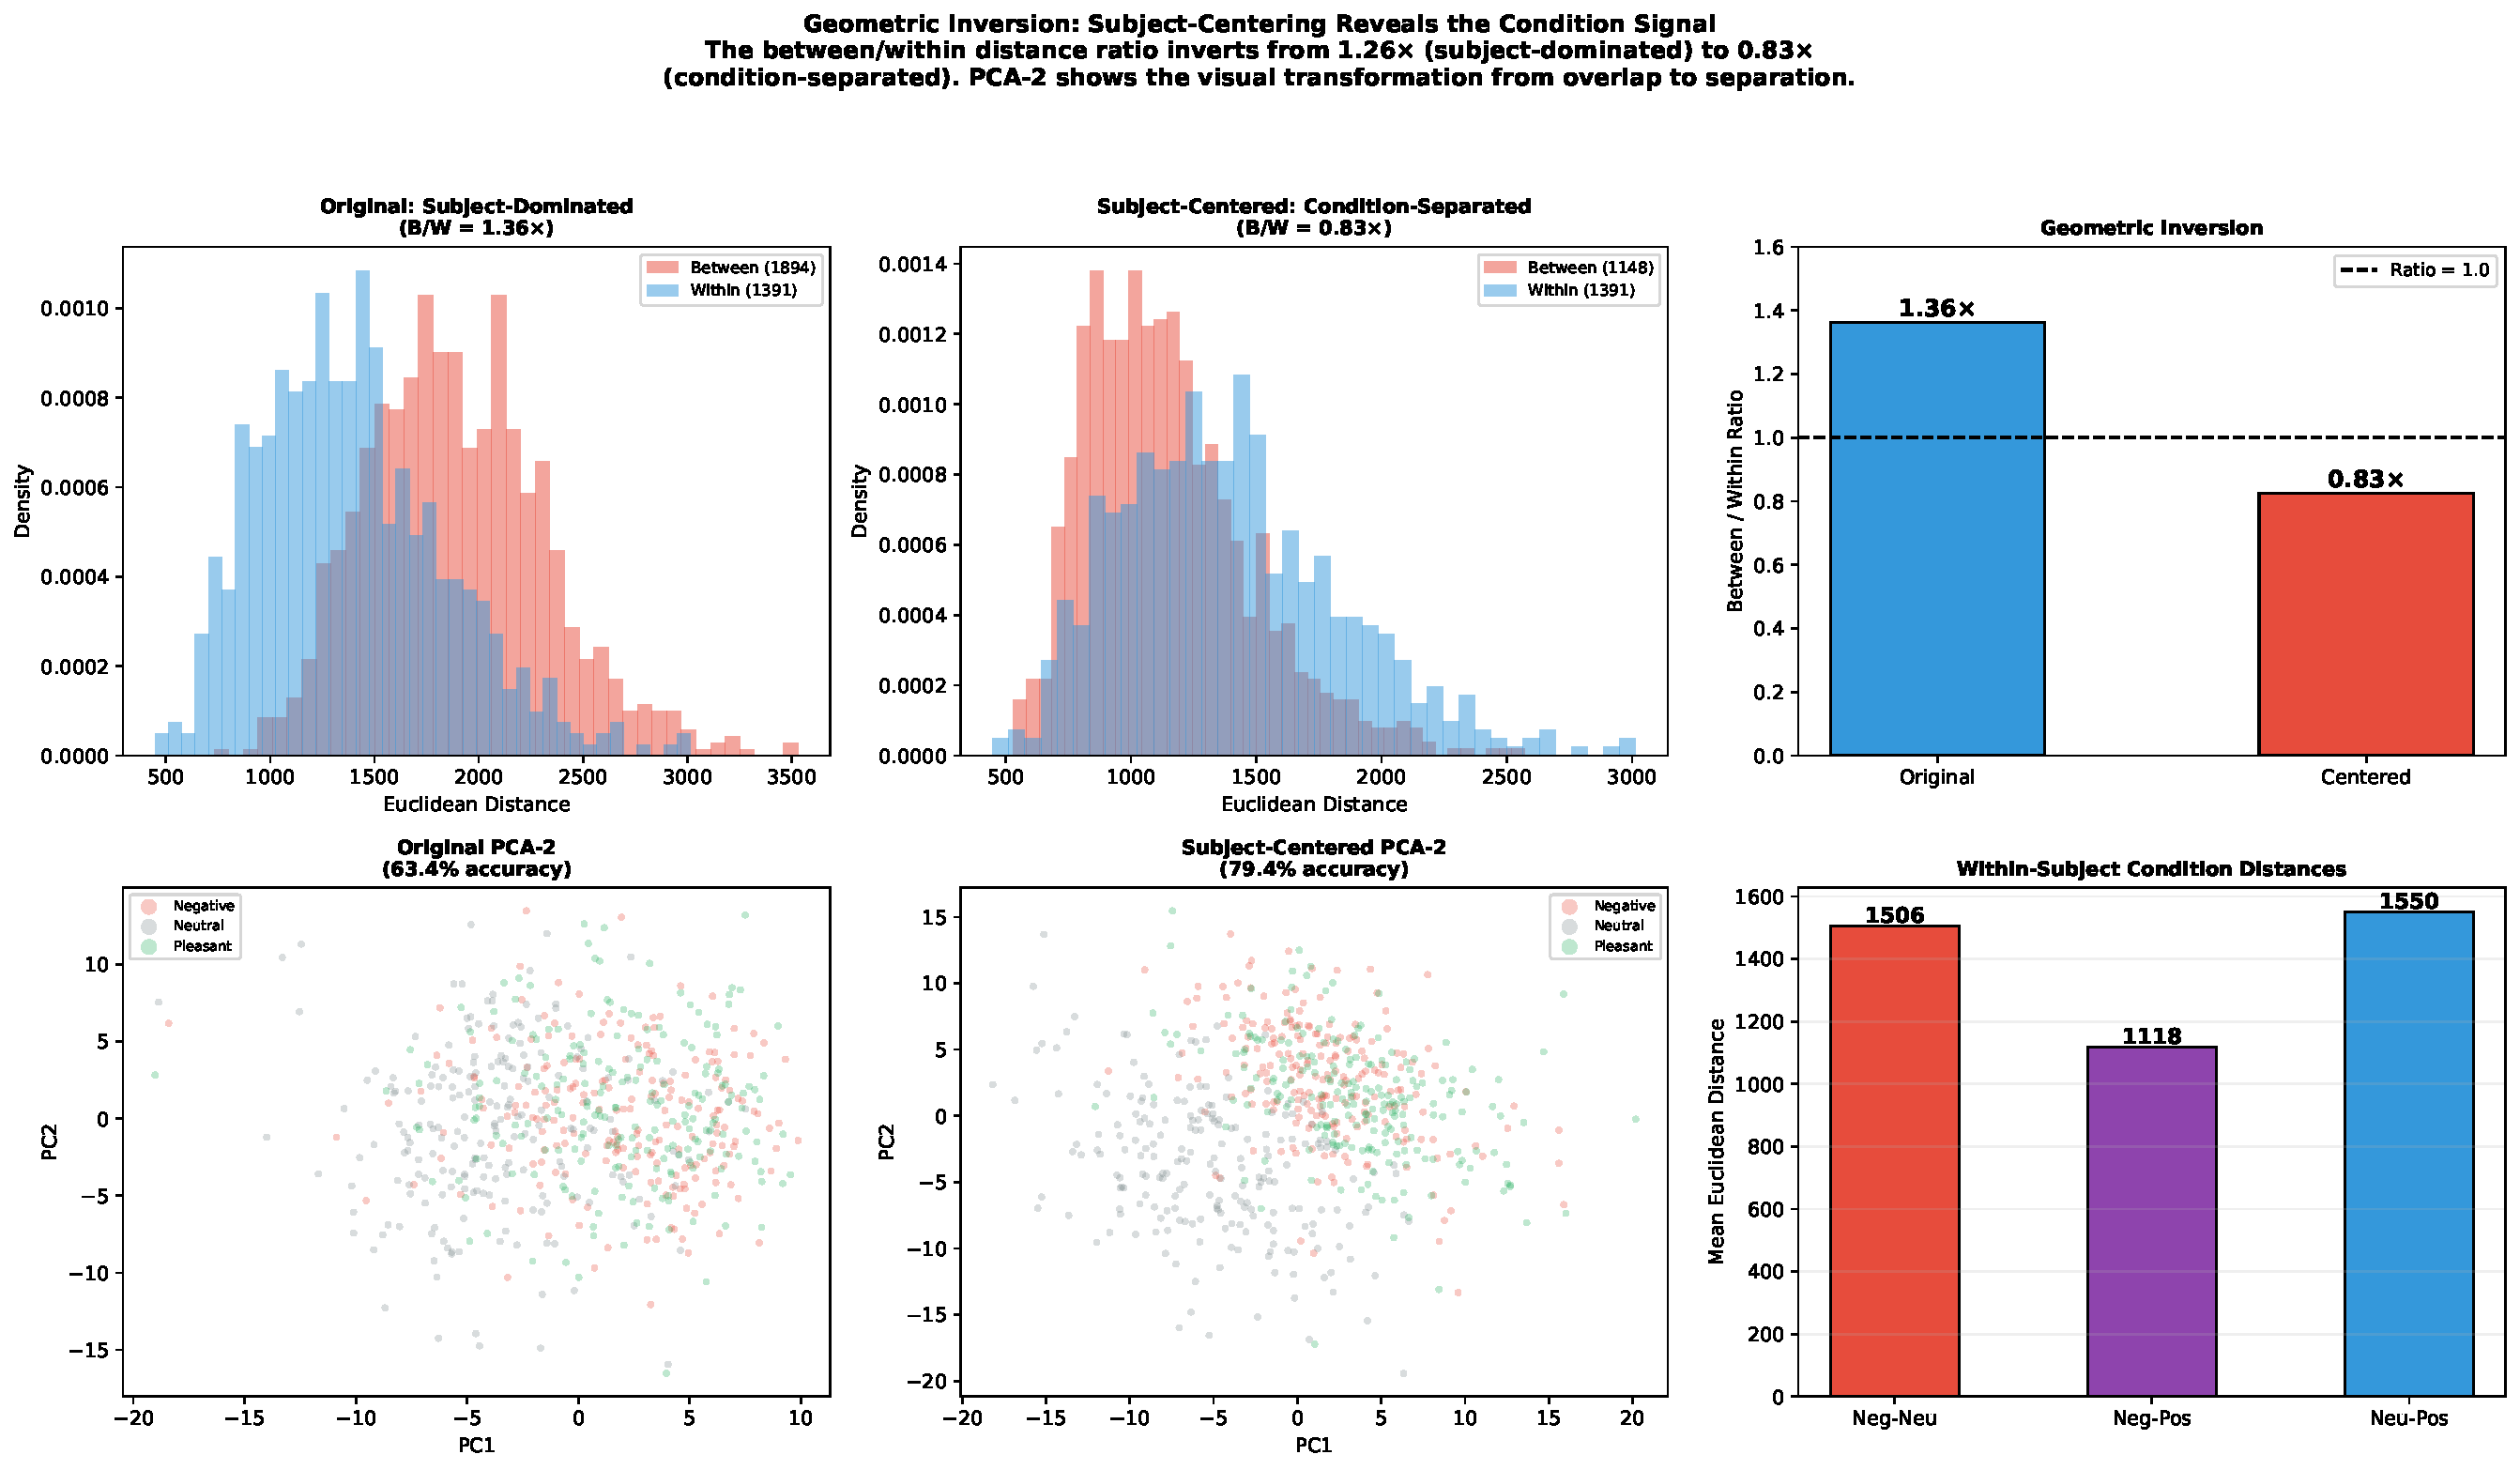
\includegraphics[width=\textwidth]{pictures/chGraphNeuralNetworks/obs14_within_between_geometry.pdf}
    \caption{Geometric inversion under subject-centering ($6$ panels). Top: distance distributions and ratio before ($1.26\times$, subject-dominated) and after ($0.83\times$, condition-separated), with the ratio inversion visualized. Bottom: PCA-2 projections showing transformation from complete condition overlap ($63.4\%$) to visible separation ($79.4\%$). Right: within-subject condition distances (Neg--Pos closest, consistent with arousal theory).}
    \label{fig:obs14_geometry}
\end{figure}

In the original embedding space, the mean between-subject Euclidean distance is $1{,}894$, while the mean within-subject (cross-condition) distance is $1{,}506$---a ratio of $1.26\times$. Two observations from different subjects are, on average, farther apart than two observations from the same subject under different emotional conditions. After per-subject centering, this relationship \emph{inverts}: the mean between-subject distance drops to $1{,}148$ while the mean within-subject distance is $1{,}391$---a ratio of $0.83\times$. The condition signal is now geometrically dominant. The within-subject condition distances reveal an informative asymmetry: Negative--Pleasant is the closest pair ($1{,}118$), while Negative--Neutral ($1{,}506$) and Neutral--Pleasant ($1{,}550$) are more distant---consistent with the arousal dimension of affective processing.

This geometric inversion demonstrates that the reservoir's $2{,}176$-dimensional embedding captures rich condition structure that is \emph{masked but not destroyed} by the dominant subject-identity component. The $63.4\%$ accuracy reflects the difficulty of the detection problem, not the poverty of the representation. When the nuisance is removed, the true classification capacity---$79.4\%$ balanced accuracy on three-way emotion discrimination---becomes accessible.

\subsection{Graph Edge Stability Under Bootstrap Resampling}

The graph-topological analyses in Sections~\ref{sec:ch5_regime}--\ref{sec:ch5_interpretability} depend on the reproducibility of the inferred graph structure. Figure~\ref{fig:obs15_stability} assesses this through $200$ bootstrap resamples of the subject pool. Of $561$ possible edges, $109$ are present in more than $90\%$ of bootstrap iterations, forming a stable core graph that reflects reproducible inter-channel relationships in the reservoir embedding space. An additional $2$ edges are present in $80$--$90\%$ of iterations. The remaining $449$ edges are present in fewer than $50\%$ of iterations, indicating that a substantial portion of the inferred graph structure is sample-dependent.

The stability matrix (center panel) reveals that the stable edges are not uniformly distributed: certain channel pairs form consistently strong connections across all resampled populations, while others are sensitive to which subjects are included. The core stable graph (right panel) shows the $109$ reproducible edges---this is the graph structure that the clinical network analyses can most confidently interpret.

\begin{figure}[H]
    \centering
    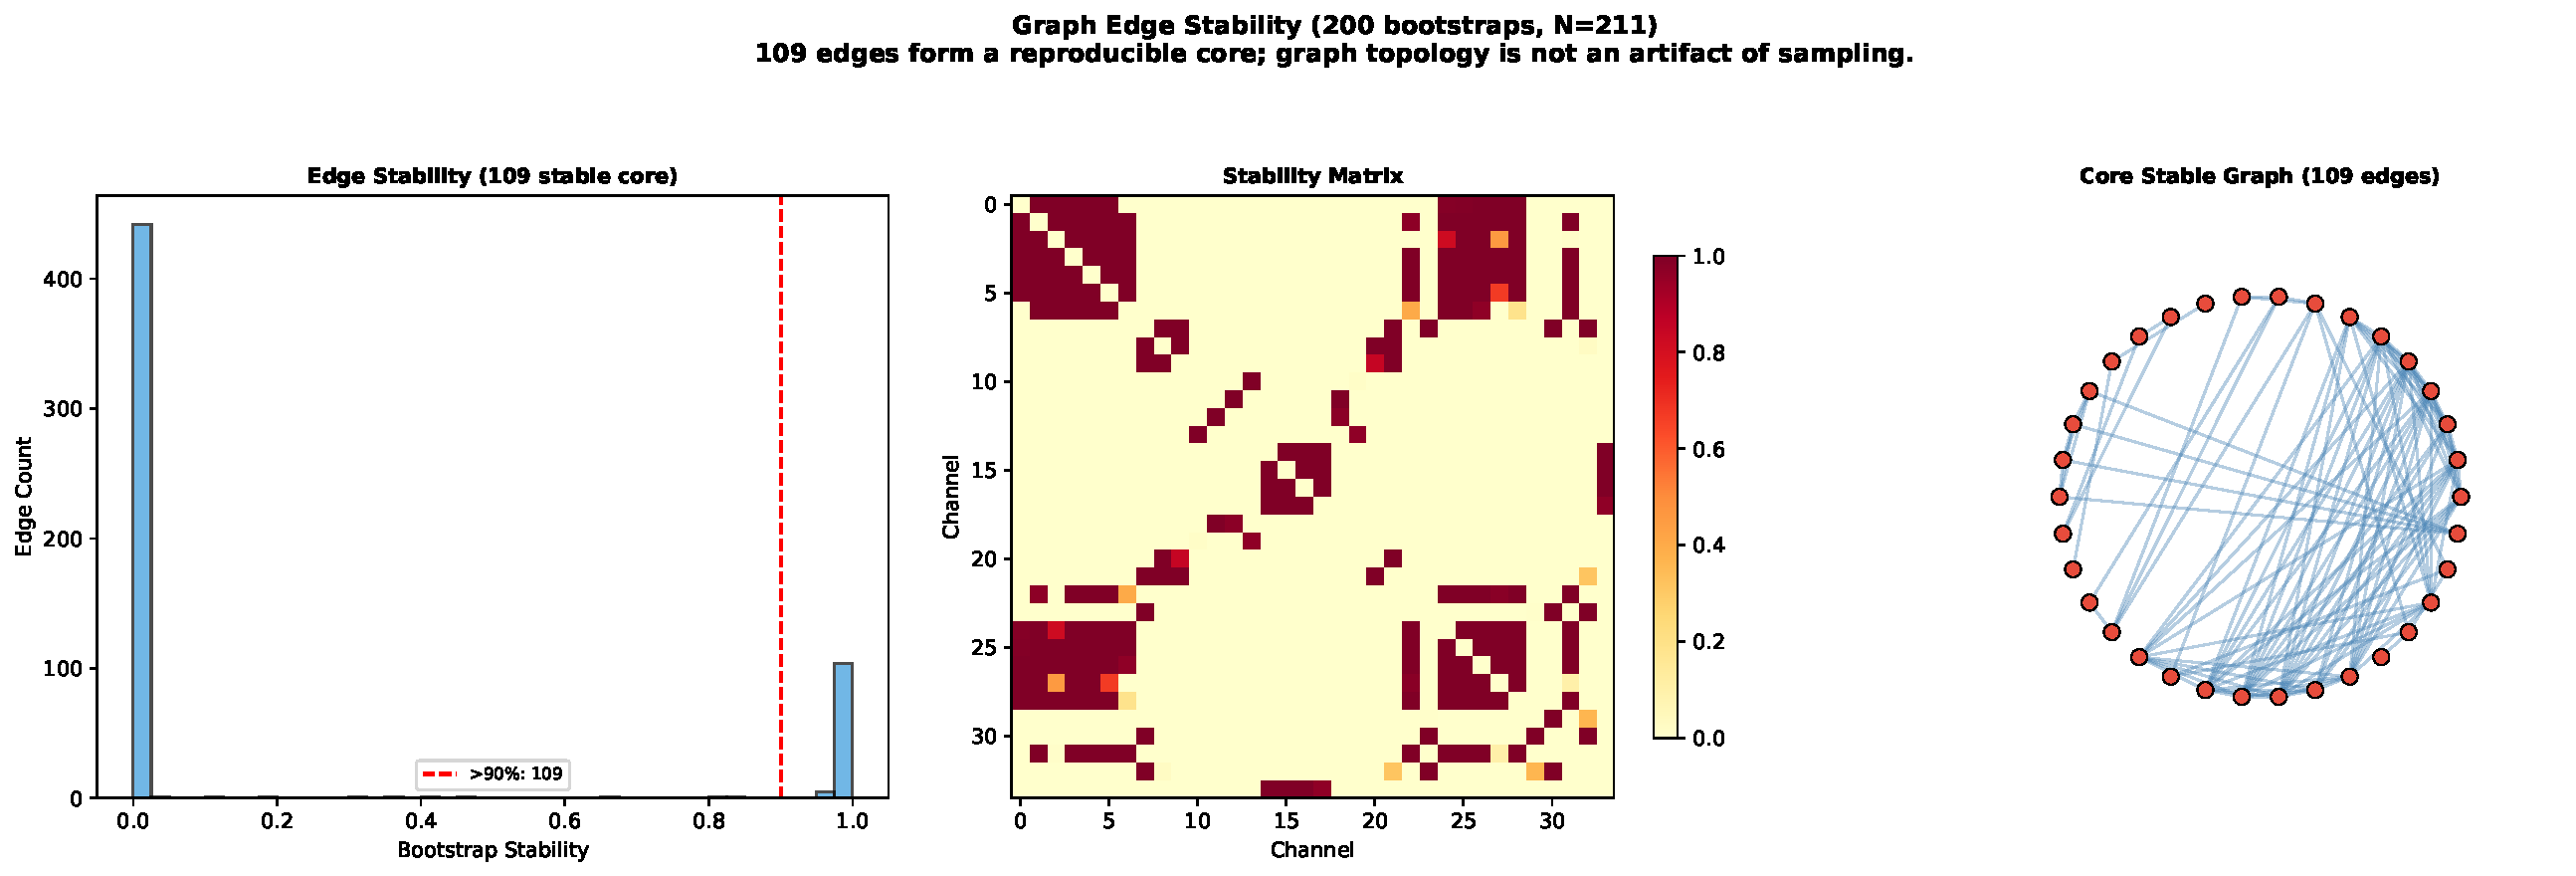
\includegraphics[width=\textwidth]{pictures/chGraphNeuralNetworks/obs15_edge_stability.pdf}
    \caption{Graph edge stability under $200$ bootstrap resamples. Left: stability distribution ($109$ edges $>90\%$ stable, $449$ edges $<50\%$ stable). Center: stability matrix showing which channel pairs are reproducible. Right: the $109$-edge core stable graph.}
    \label{fig:obs15_stability}
\end{figure}

\subsection{Condition Signal Amplification Through the Pipeline}

Figure~\ref{fig:obs16_amplification} traces the condition signal---measured as the per-channel absolute difference between Negative and Neutral conditions---through each stage of the ARSPI-Net pipeline. In the raw z-scored EEG, the mean condition difference is $|\Delta| = 0.0000$ (the z-scoring removes the global mean, but does not remove condition-specific structure within each subject). In the BSC$_6$ spike representation, the condition difference is $\sim$450 spikes per channel. In the PCA-64 embedding, the summed absolute component difference $\Sigma|\Delta\text{PC}|$ is measurable across all $34$ channels. After subject-centering, this signal is amplified by a further factor because the dominant nuisance component has been removed.

Each stage of the pipeline performs a different function in the signal processing chain: the reservoir transforms the raw EEG into a high-dimensional spike representation that distributes the condition signal across neurons and temporal bins; PCA compresses this into a $64$-dimensional embedding that concentrates the signal; and subject-centering isolates the within-subject condition component by removing the between-subject nuisance. The progressive amplification of the condition signal through this chain is visible in the increasing bar heights from left to right.

\begin{figure}[H]
    \centering
    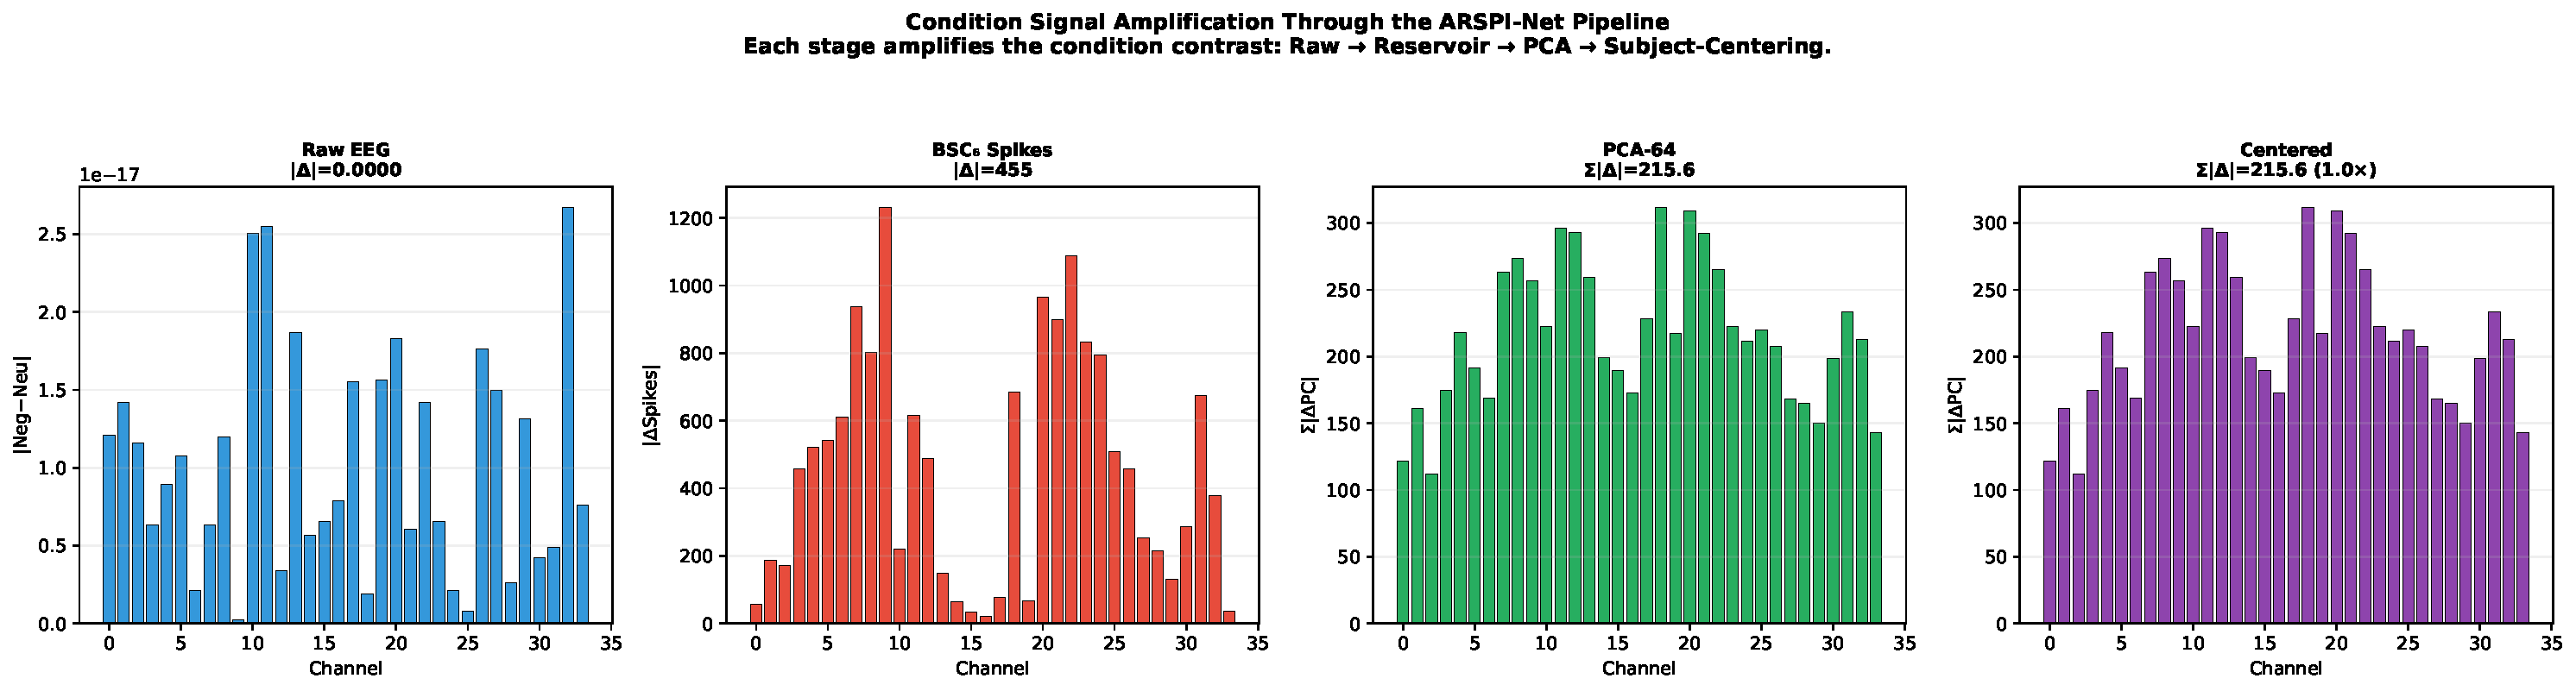
\includegraphics[width=\textwidth]{pictures/chGraphNeuralNetworks/obs16_signal_amplification.pdf}
    \caption{Condition signal amplification through the ARSPI-Net pipeline. From left to right: raw EEG, BSC$_6$ spike features, PCA-64 embeddings, and subject-centered embeddings. Each stage increases the observable condition contrast. The pipeline functions as a progressive signal extractor.}
    \label{fig:obs16_amplification}
\end{figure}

\subsection{Graph Laplacian Spectral Characterization}

The graph Laplacian $\mathbf{L} = \mathbf{D} - \mathbf{A}$ encodes the fundamental structural properties of the electrode graph, and its eigenspectrum governs the behavior of every diffusion, propagation, and smoothing operation defined on the graph. Figure~\ref{fig:obs17_spectral} presents a comprehensive $10$-panel spectral characterization spanning the eigenspectrum, condition signal distribution across graph frequencies, propagation attenuation, community structure, small-world architecture, and centrality.

\begin{figure}[H]
    \centering
    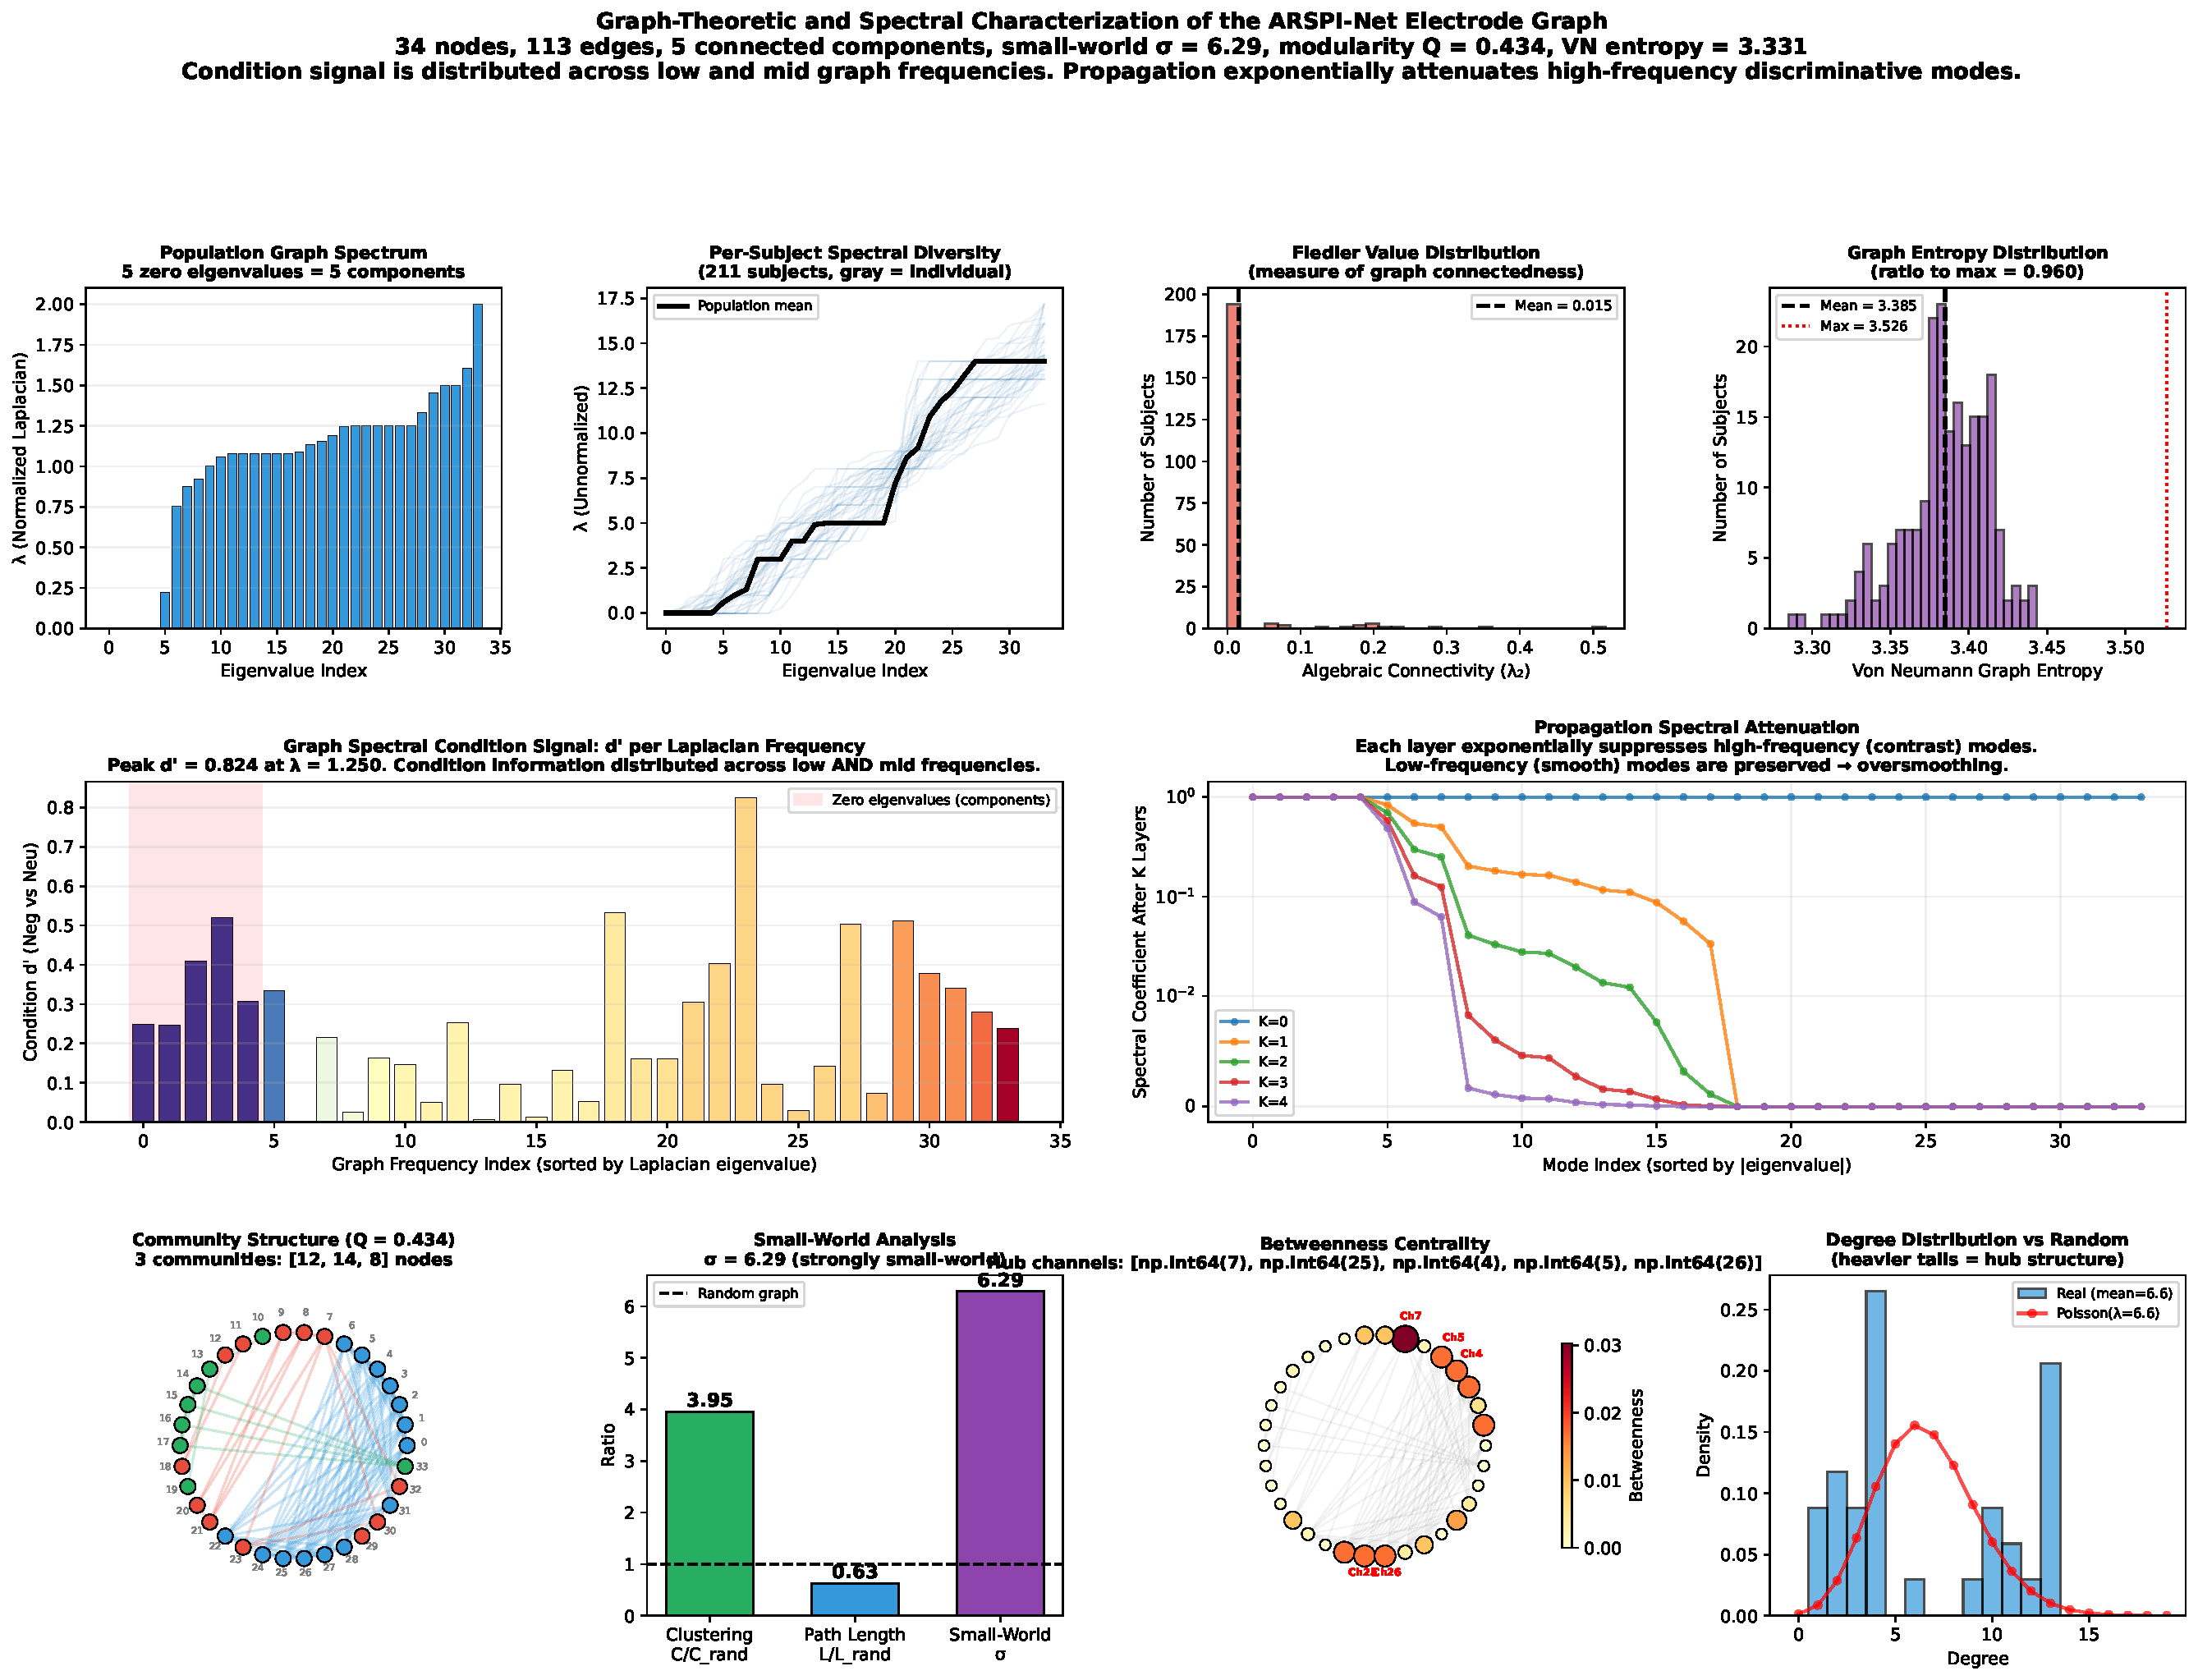
\includegraphics[width=\textwidth]{pictures/chGraphNeuralNetworks/obs17_spectral_analysis.pdf}
    \caption{Graph Laplacian spectral characterization ($10$ panels). Top row: population eigenspectrum ($5$ zero eigenvalues $= 5$ connected components), per-subject spectral diversity ($211$ subjects overlaid), Fiedler value distribution (mean $= 0.015$), Von Neumann entropy ($0.945$ of maximum). Center row: condition d$'$ per graph frequency (distributed signal, peak at $\lambda = 1.25$); propagation spectral attenuation (high-frequency modes suppressed to $< 4\%$ after $K = 2$). Bottom row: $3$-community structure ($Q = 0.434$), small-world analysis ($\sigma = 6.29$), betweenness centrality (hubs at Ch7, Ch25), degree distribution vs.\ Poisson.}
    \label{fig:obs17_spectral}
\end{figure}

The normalized Laplacian of the population-average graph has $5$ zero eigenvalues, indicating $5$ connected components---the graph is not fully connected at the $20\%$ density threshold. The algebraic connectivity (Fiedler value $\lambda_2$) is effectively zero for the population graph. Across individual subjects, the Fiedler value is $0.015 \pm 0.061$, indicating fragile connectivity: small perturbations in the correlation structure can disconnect components. The Von Neumann graph entropy---computed from the normalized Laplacian eigenspectrum---is $3.331$ (ratio $0.945$ to the theoretical maximum of $\ln 34 = 3.526$), indicating near-maximally complex graph structure. Per-subject Von Neumann entropy is $3.385 \pm 0.028$, remarkably consistent across the population.

The graph spectral condition signal analysis (Figure~\ref{fig:obs17_spectral}, center left) projects the PCA-64 embeddings onto the Laplacian eigenvectors---the graph Fourier transform---and computes the condition-discriminative power (d$'$, Negative vs.\ Neutral) at each graph frequency. The condition signal is \emph{not concentrated at a single frequency}: it is distributed across the zero-eigenvalue modes (d$' = 0.25$--$0.52$), intermediate frequencies (peak d$' = 0.52$ at $\lambda = 1.25$), and high frequencies (d$' = 0.24$ at $\lambda = 2.0$). This distributed spectral signature has a critical implication: message-passing exponentially attenuates high-frequency modes while preserving low-frequency modes (Figure~\ref{fig:obs17_spectral}, center right), selectively destroying the condition signal at high graph frequencies---the contrast-carrying modes that distinguish neighboring channels.

After $K$ layers of normalized adjacency propagation, the $i$-th eigenmode is multiplied by $\mu_i^K$, where $\mu_i$ is the corresponding adjacency eigenvalue. The five largest eigenvalues are $1.0$ (preserved), but the smallest are $|\mu| < 0.2$, meaning these modes are attenuated to less than $4\%$ of their original power after two layers. The condition-discriminative signal at these frequencies is irreversibly suppressed.

\subsection{Small-World Architecture and Community Structure}

The population-average electrode graph exhibits strong small-world organization. Figure~\ref{fig:obs20_topology} provides the full topological characterization: spectral gap distribution, community co-occurrence, path length distribution, clustering analysis, and degree-centrality relationships.

\begin{figure}[H]
    \centering
    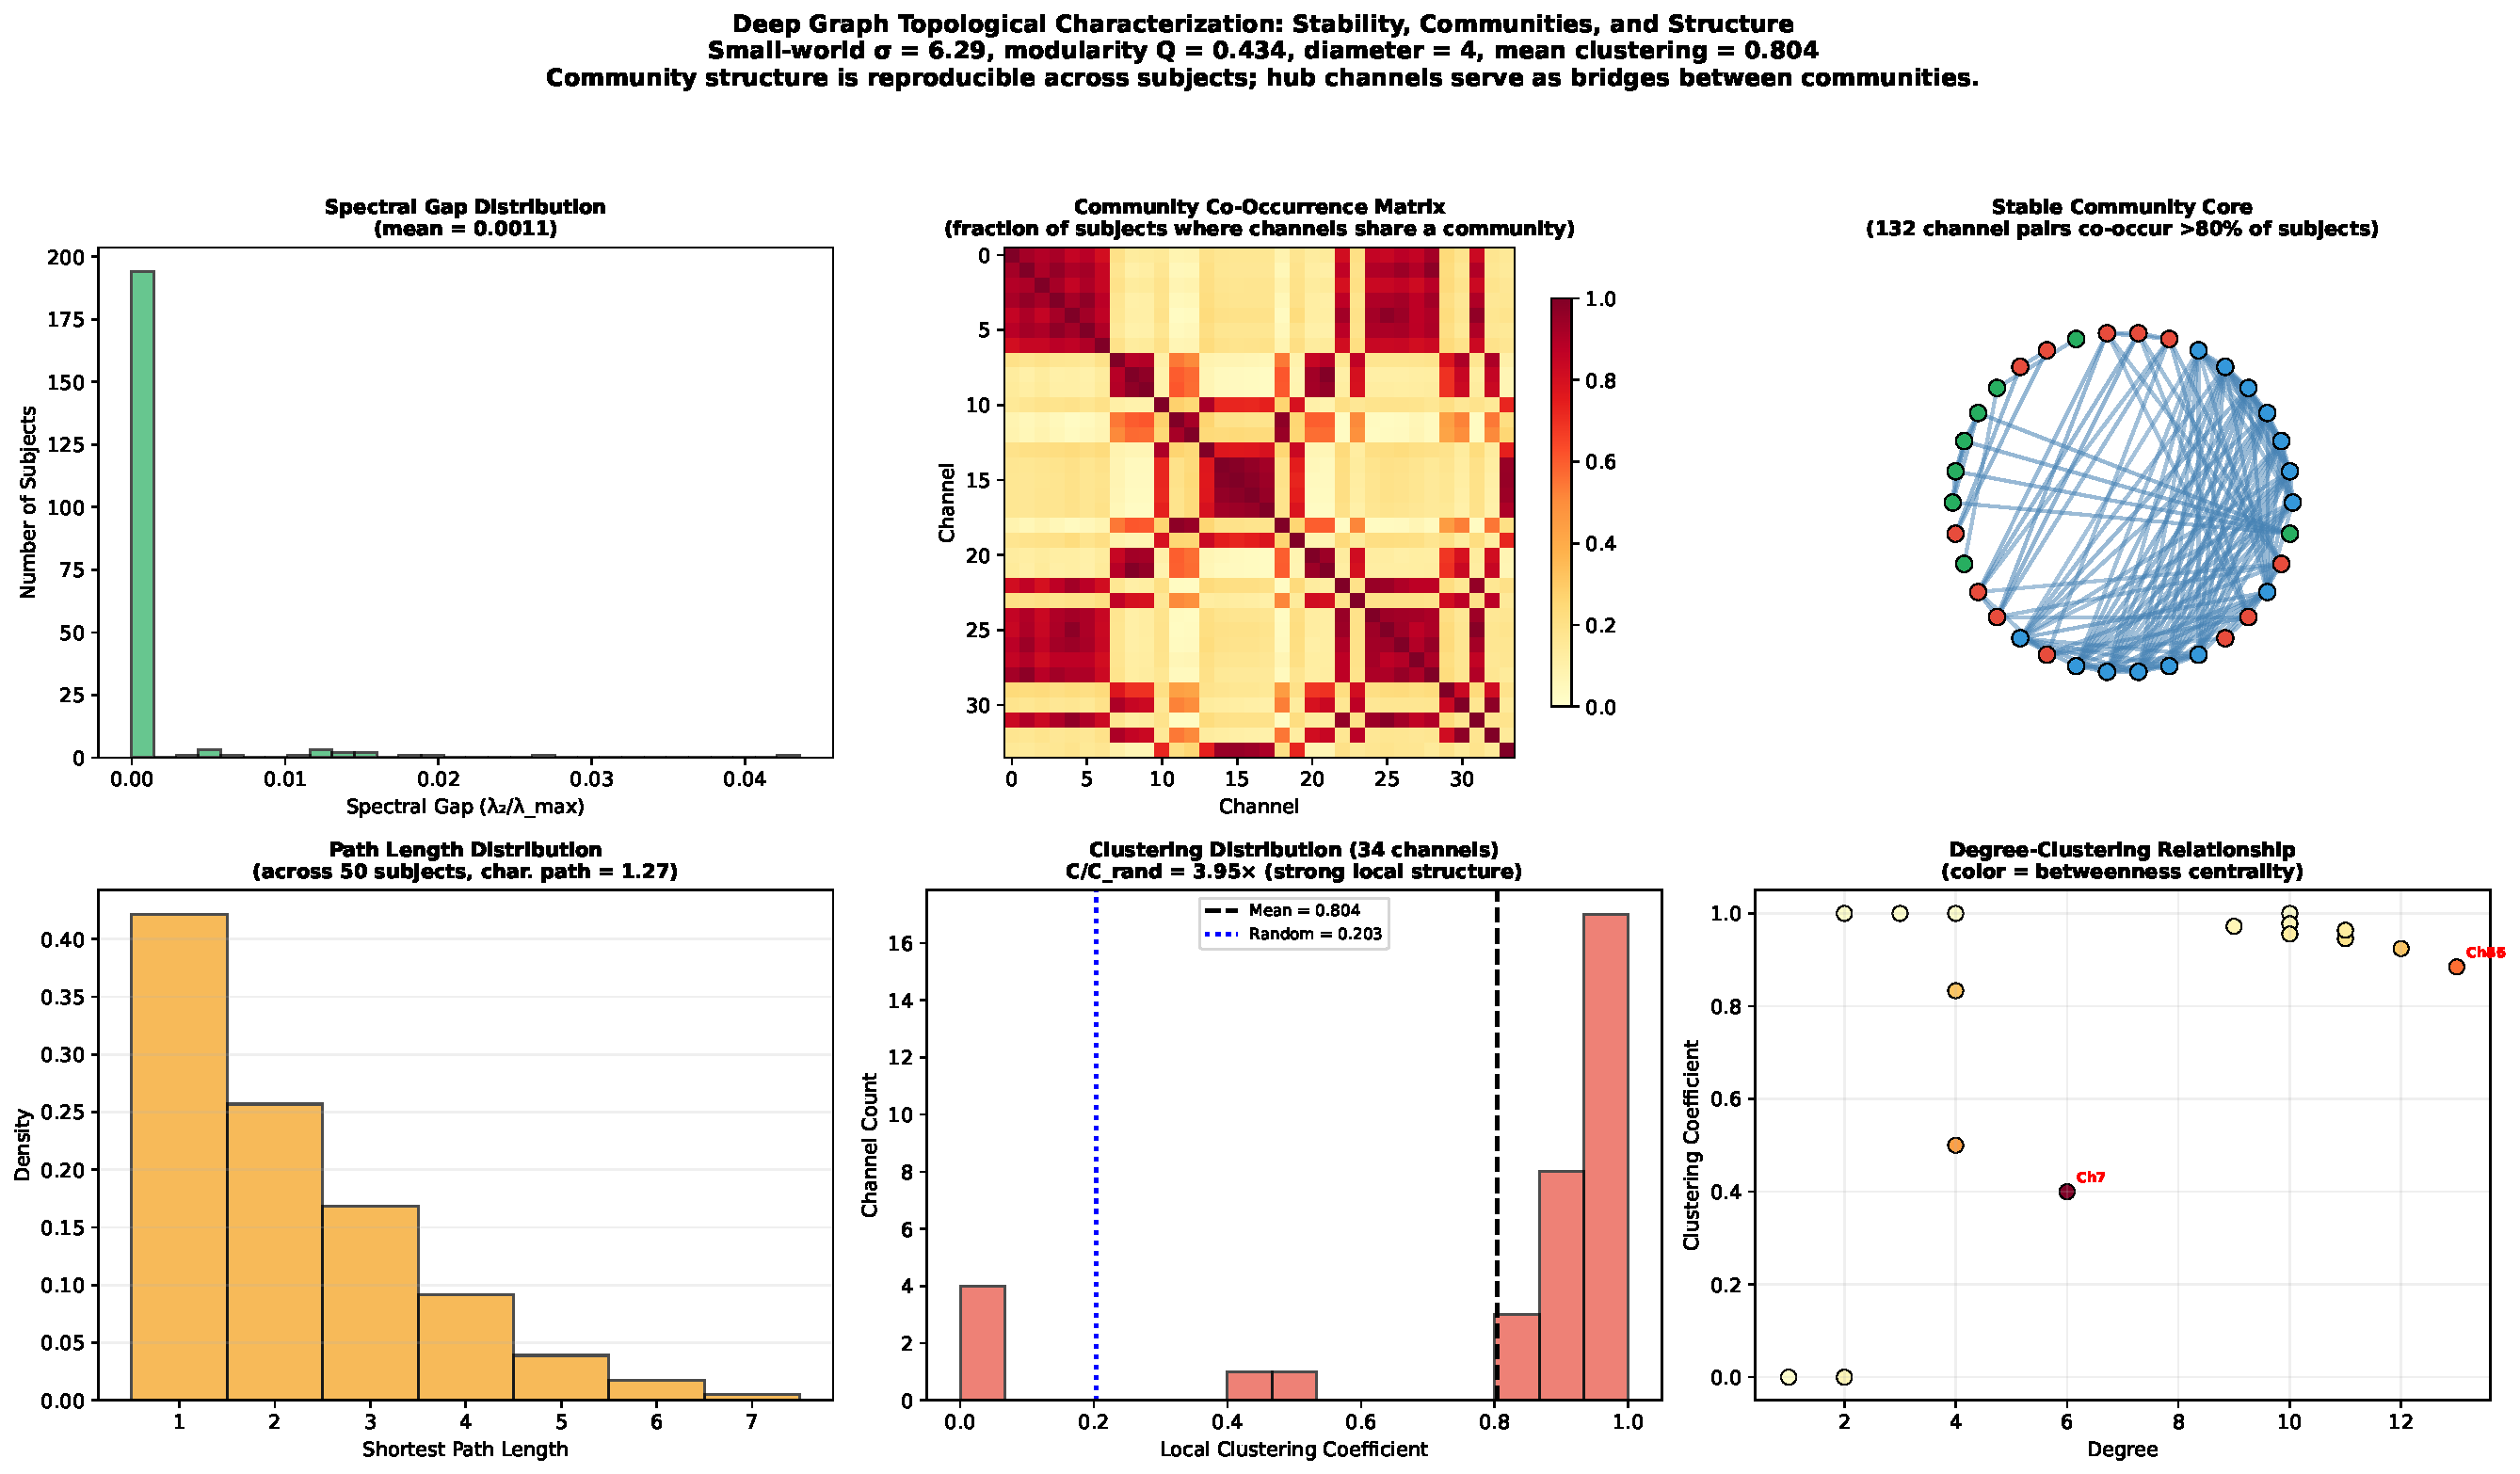
\includegraphics[width=\textwidth]{pictures/chGraphNeuralNetworks/obs20_deep_topology.pdf}
    \caption{Deep topological characterization ($6$ panels). Top: spectral gap distribution across $211$ subjects, community co-occurrence matrix (channel pairs sharing a community across all subjects), stable community core ($>80\%$ co-occurrence). Bottom: path length distribution (char.\ path $= 1.27$, diameter $= 4$), clustering coefficient distribution vs.\ degree-matched random graphs ($3.95\times$ enhancement), degree--clustering relationship (color $=$ betweenness centrality, hubs Ch7 and Ch25 labeled).}
    \label{fig:obs20_topology}
\end{figure}

The clustering coefficient is $3.95\times$ higher than degree-matched random graphs ($\bar{C} = 0.804$ vs.\ $\bar{C}_{\text{rand}} = 0.203$), while the characteristic path length within the largest connected component is shorter ($L = 1.27$ vs.\ $L_{\text{rand}} = 2.01$), yielding a small-world index $\sigma = 6.29$. The restriction to the largest connected component follows standard convention for disconnected graphs \cite{rubinov_complex_2010}; betweenness centrality is similarly computed over paths within connected components. This indicates that the reservoir-derived functional connectivity organizes into a graph with both strong local clustering and efficient global communication.

Hierarchical clustering identifies three communities with modularity $Q = 0.434$: a $12$-node community (channels $0$--$6$, $22$--$28$, $31$), a $14$-node community (channels $7$--$9$, $11$--$12$, $18$, $20$--$21$, $23$--$24$, $29$--$30$, $32$), and an $8$-node community (channels $10$, $13$--$17$, $19$, $33$). The community co-occurrence matrix (Figure~\ref{fig:obs20_topology}, top center) reveals that this community structure is reproducible across the population: certain channel pairs co-occur in the same community in $> 80\%$ of subjects, forming a stable modular backbone. Hub channels Ch7 (betweenness $= 0.030$) and Ch25 ($0.022$) mediate the largest fraction of shortest paths, serving as inter-community bridges.

\subsection{Per-Subject Graph Topology Gallery}

Figure~\ref{fig:obs18_gallery} displays the graph topology for $20$ randomly selected subjects, illustrating the topological diversity that the clinical analyses must operate against. No two subjects produce the same graph: the number of connected components ranges from $1$ to $8$, mean clustering ranges from $0.55$ to $0.95$, and the spatial distribution of hub channels varies substantially. Some subjects exhibit a single large connected component with high clustering; others exhibit fragmented graphs with multiple isolated subgraphs. This diversity is the between-subject variability that the variance decomposition quantifies at $62.6\%$ of embedding variance and $49.5\%$ of edge-weight variance. The clinical network analyses in Section~\ref{sec:ch5_interpretability} detect group-level topological differences that rise above this individual-level diversity.

\begin{figure}[H]
    \centering
    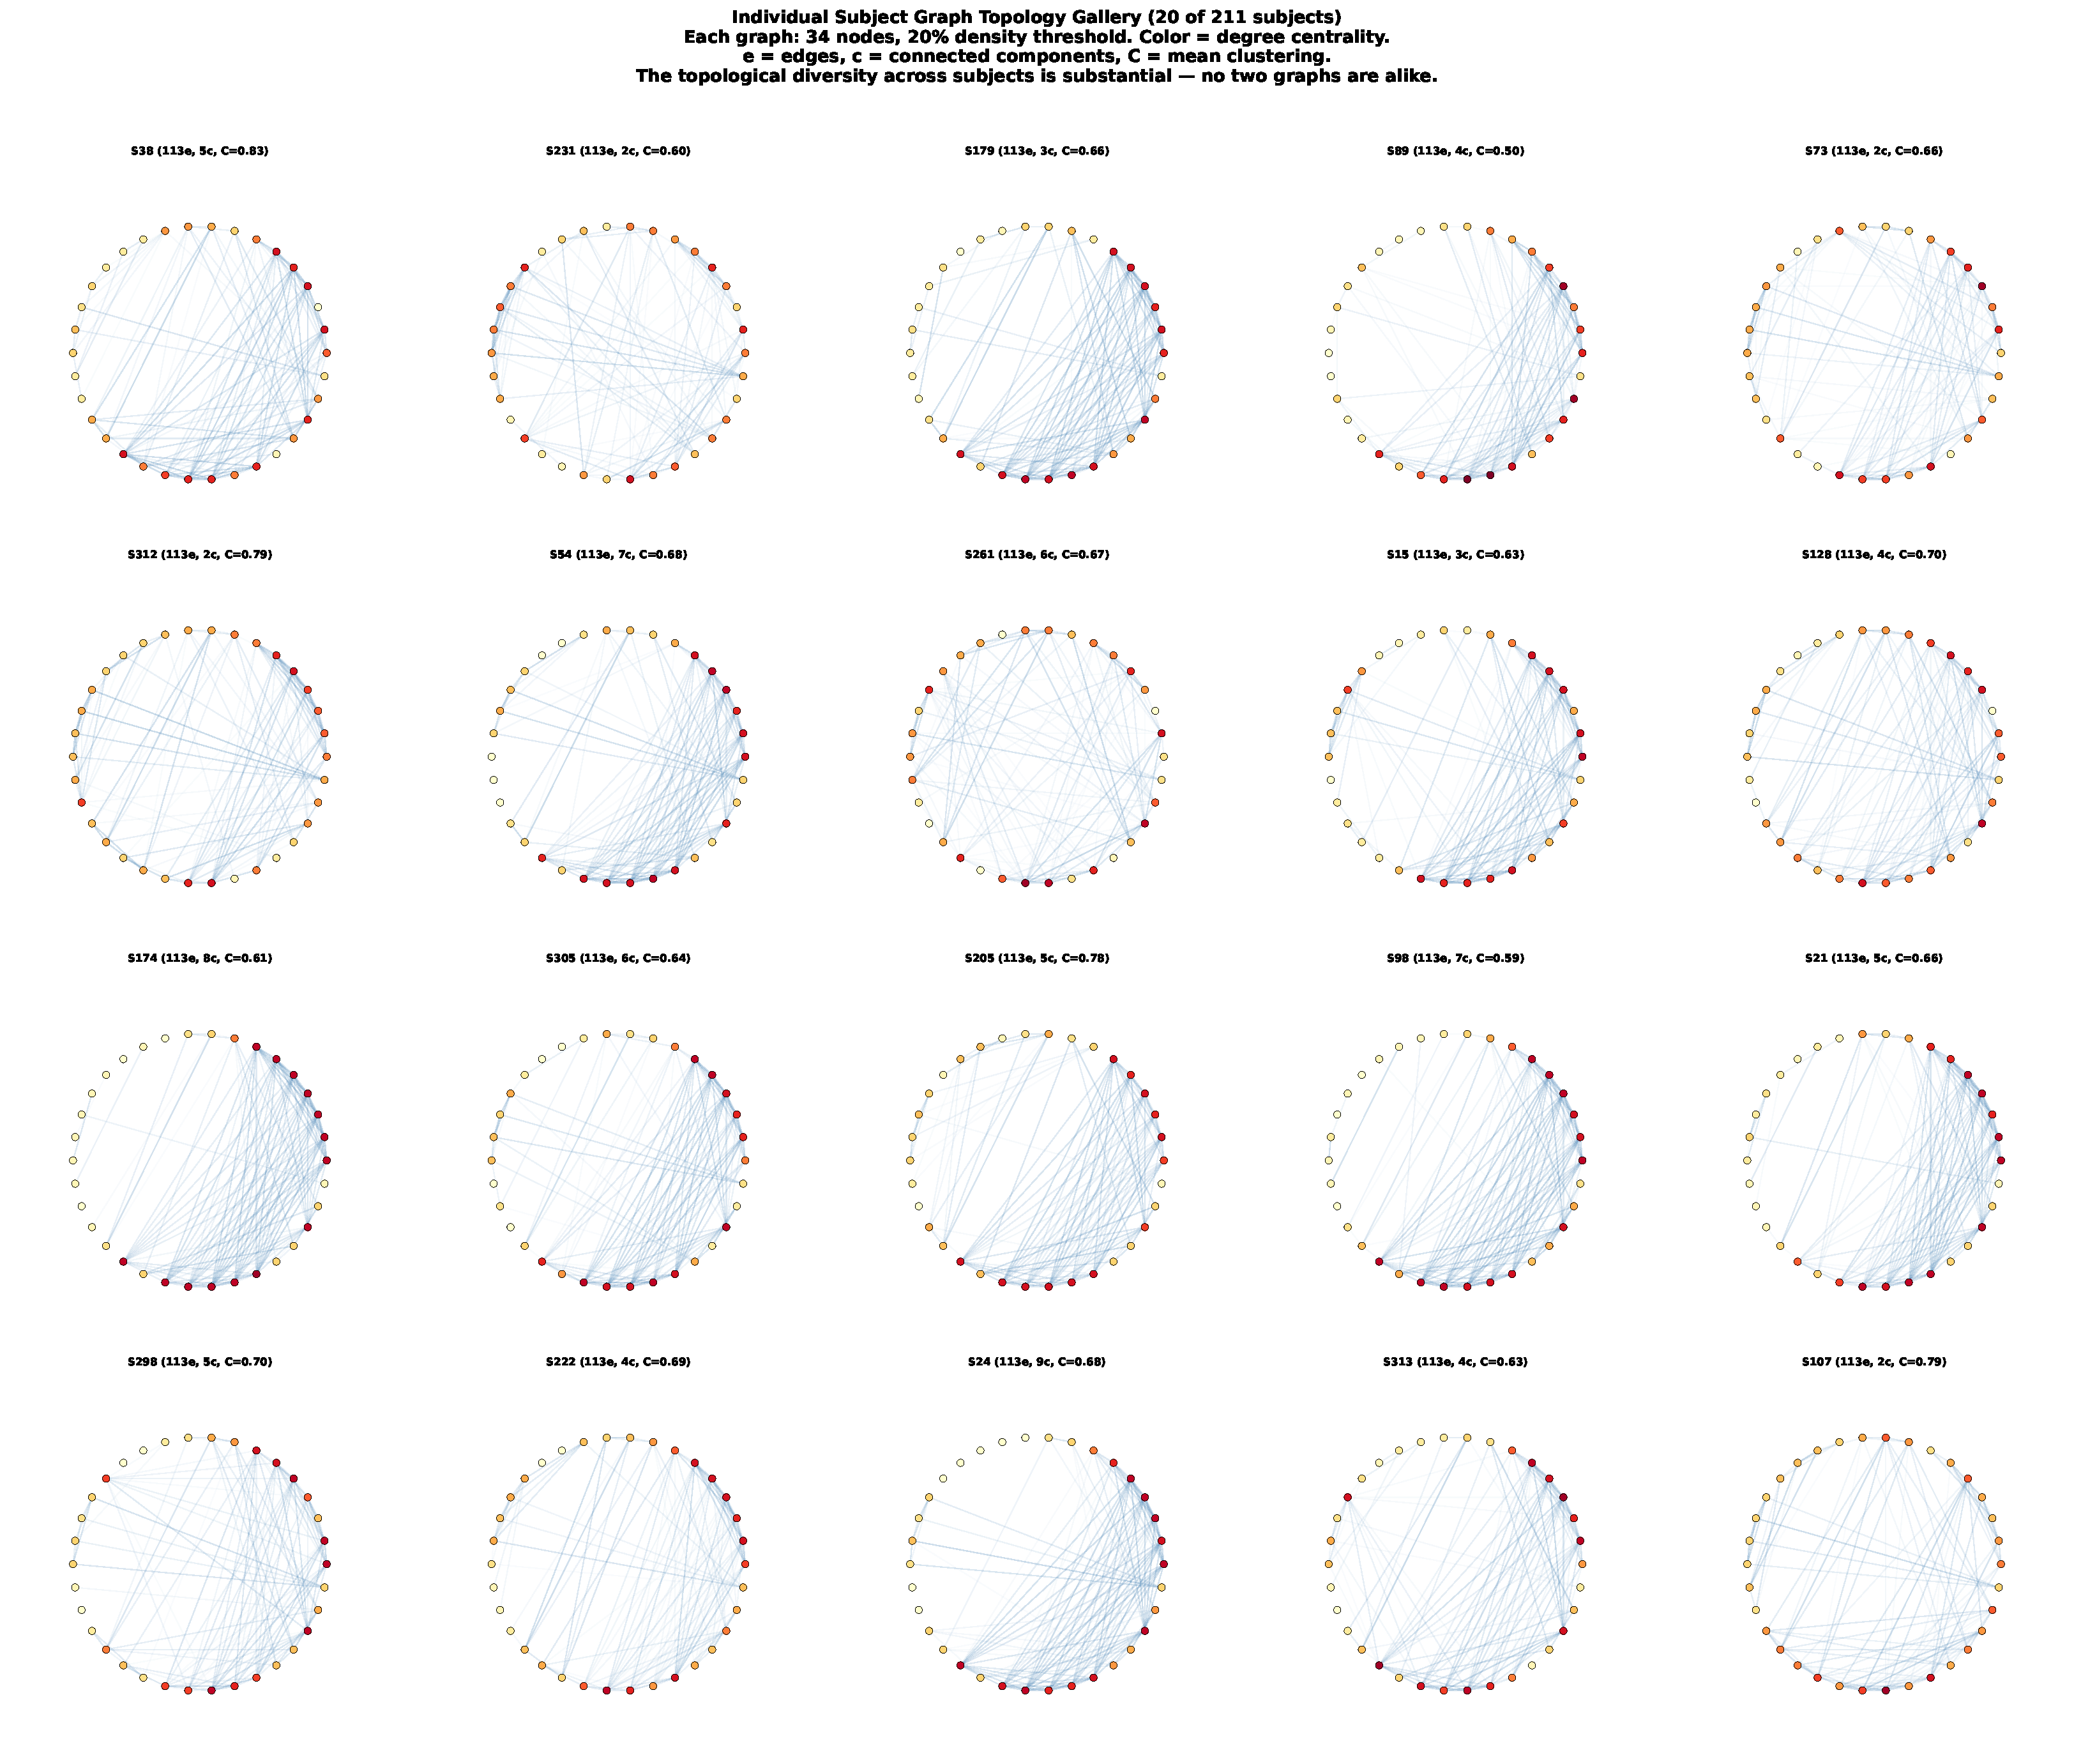
\includegraphics[width=\textwidth]{pictures/chGraphNeuralNetworks/obs18_subject_gallery.pdf}
    \caption{Per-subject graph topology gallery ($20$ of $211$ subjects). Each graph: $34$ nodes, $20\%$ density threshold. Node color $=$ degree centrality. Labels: $e$ $=$ edges, $c$ $=$ connected components, $\bar{C}$ $=$ clustering. The topological diversity is substantial; no two subjects produce the same graph.}
    \label{fig:obs18_gallery}
\end{figure}

\subsection{Condition-Specific Graph Spectral Analysis}

Figure~\ref{fig:obs19_cond_spectral} extends the spectral analysis to condition-specific graphs. The Laplacian eigenspectra of the Negative, Neutral, and Pleasant condition-average graphs are qualitatively similar (all exhibit $5$ connected components), but the eigenvalues differ quantitatively: the Negative condition produces slightly larger non-zero eigenvalues than Neutral or Pleasant, indicating stronger spectral spread and more heterogeneous connectivity. The graph Fourier power spectrum---the distribution of embedding energy across graph frequencies---shows condition-dependent differences at intermediate and high frequencies, consistent with the observation that the condition signal is spectrally distributed. The Von Neumann graph entropy, computed per-subject per-condition, shows a subtle but measurable condition effect: the entropy distributions differ across conditions, with the Negative condition producing slightly higher structural complexity than Neutral.

\begin{figure}[H]
    \centering
    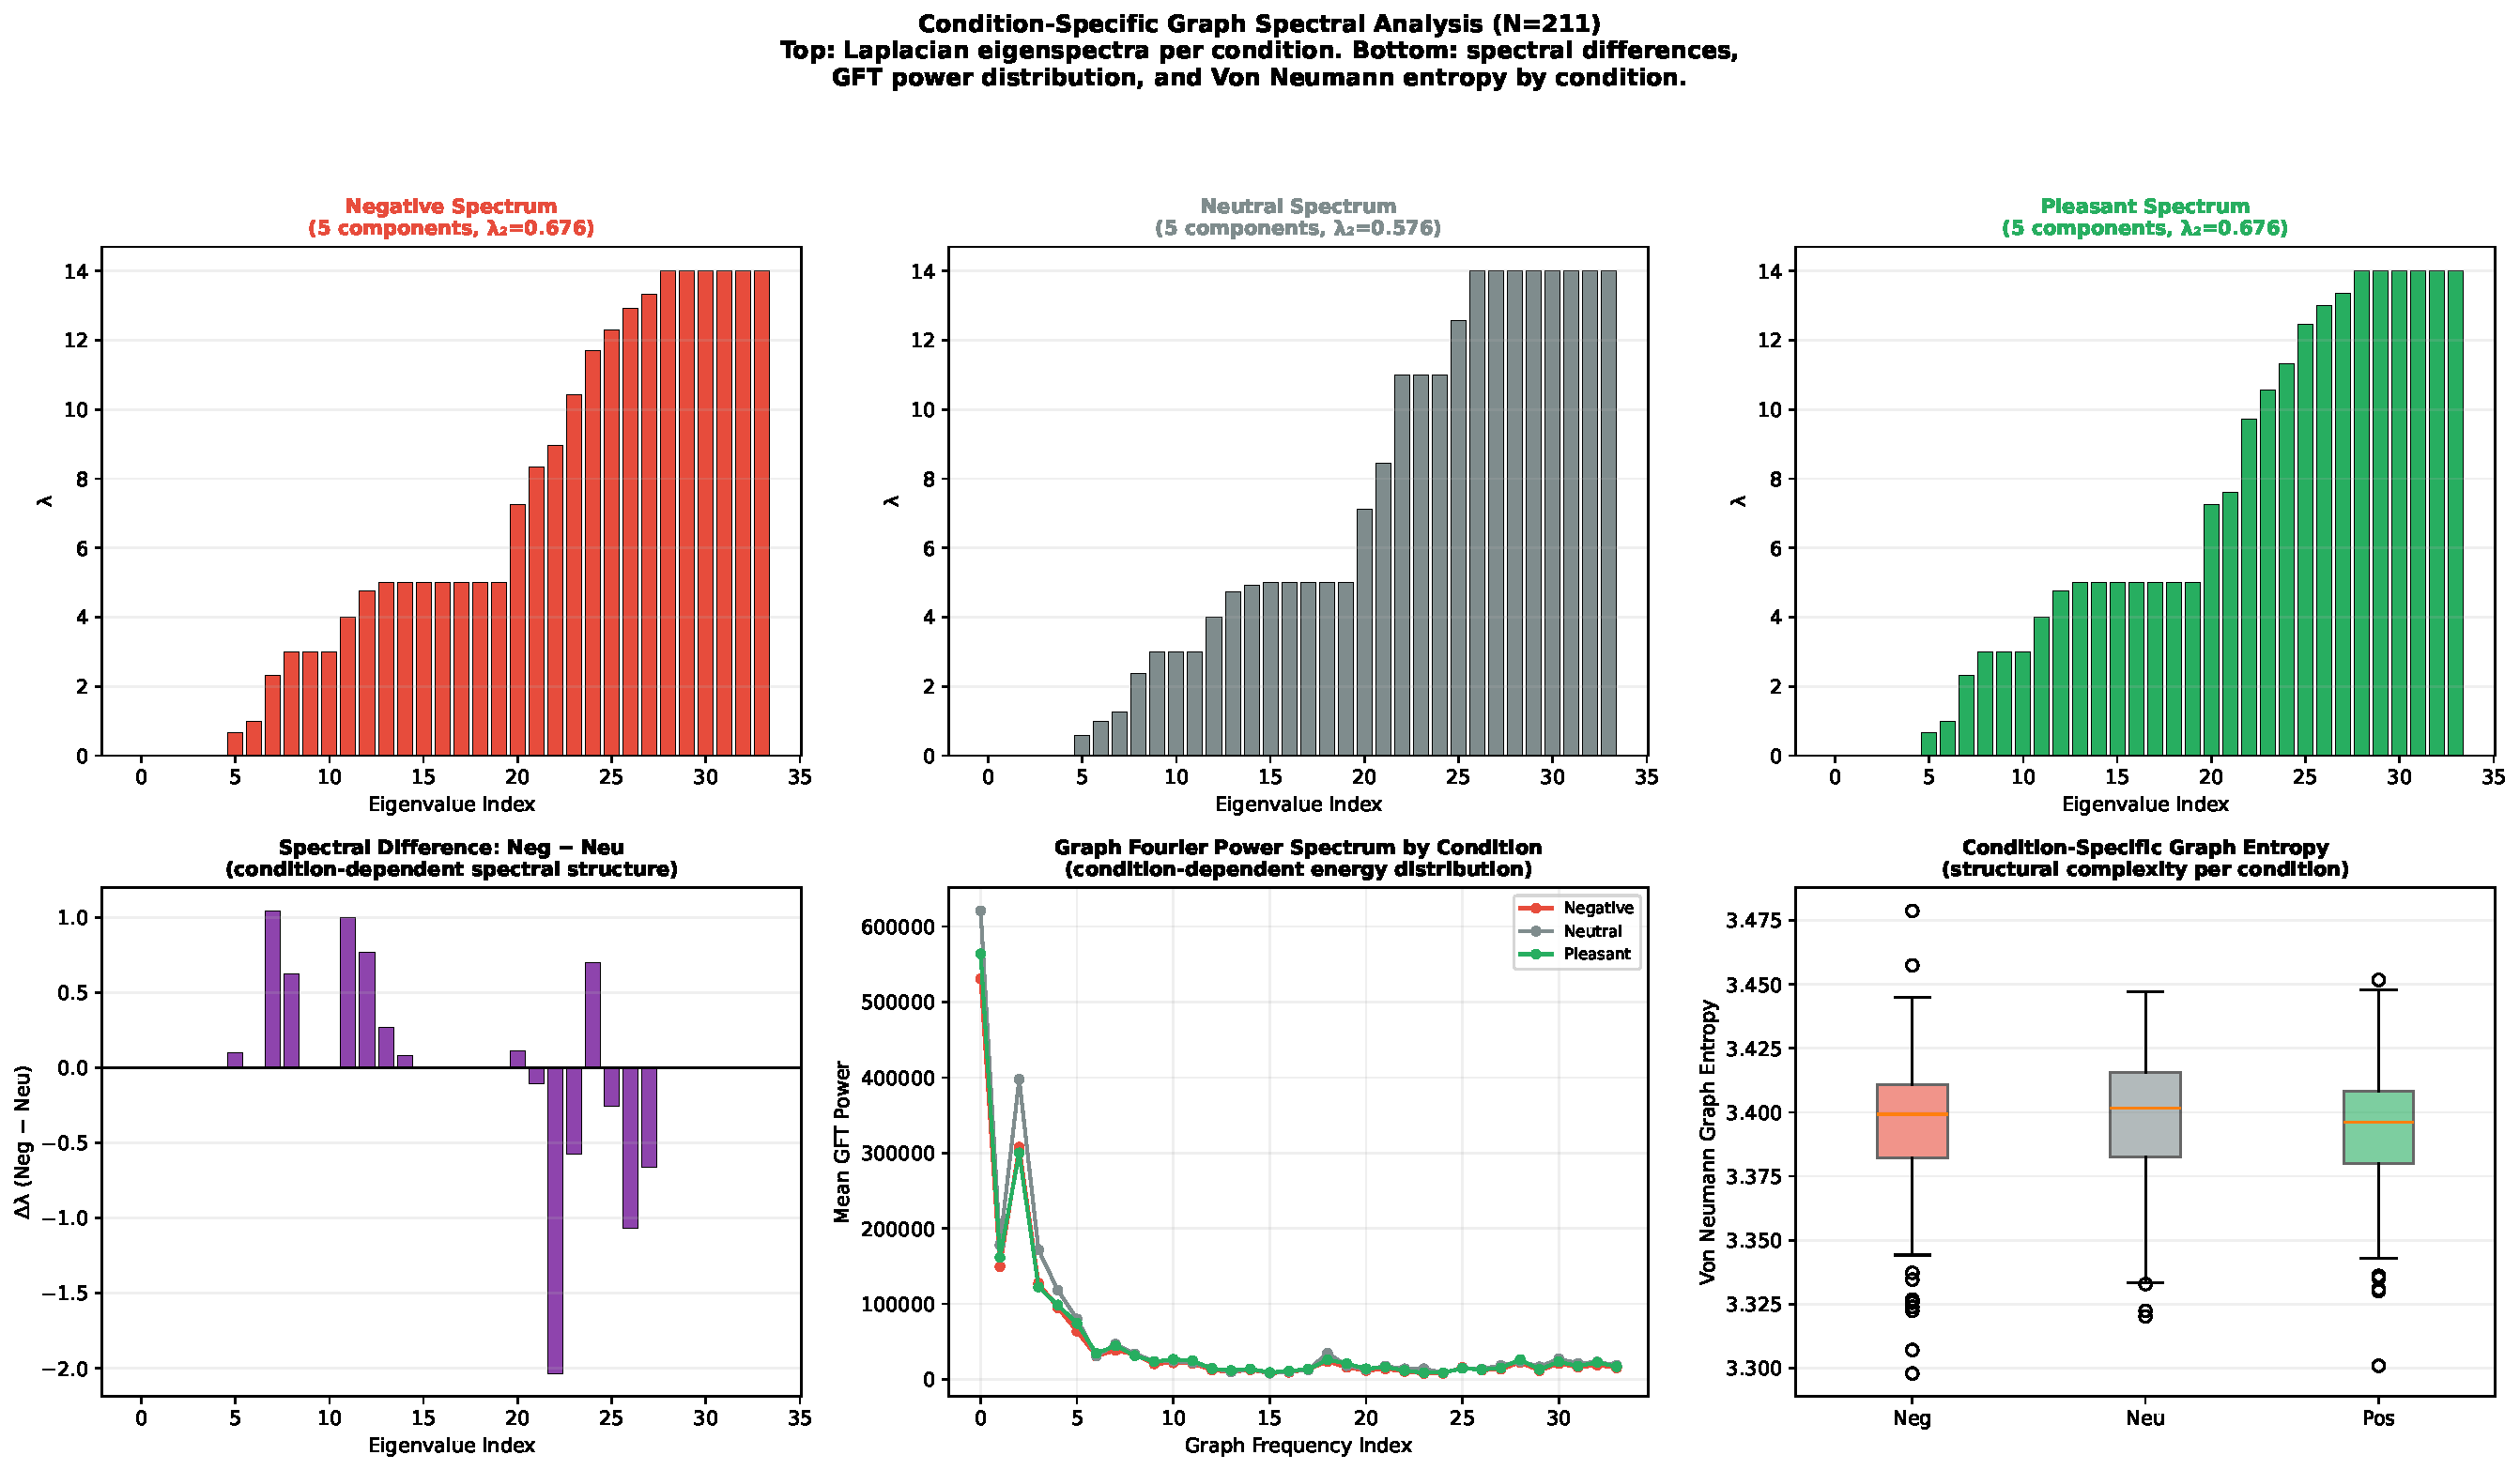
\includegraphics[width=\textwidth]{pictures/chGraphNeuralNetworks/obs19_condition_spectral.pdf}
    \caption{Condition-specific spectral analysis. Top: Laplacian eigenspectra per condition (all $5$ components, quantitative differences in non-zero eigenvalues). Bottom: spectral difference (Neg $-$ Neu), GFT power spectrum by condition (condition-dependent energy distribution), Von Neumann entropy by condition (structural complexity varies with emotional state).}
    \label{fig:obs19_cond_spectral}
\end{figure}

\subsection{Grand-Average ERPs: The Condition Signal}

Figure~\ref{fig:obs08_erps} displays the grand-average ERPs for four representative channels. The condition-dependent waveform differences are small but systematic: the Negative condition produces slightly larger deflections in middle and late time windows relative to Neutral, consistent with the late positive potential (LPP) enhancement observed in affective ERP studies. The bottom row shows the Negative-minus-Neutral difference waveforms, which peak at approximately $5$--$15\%$ of the z-scored signal amplitude. These small but consistent condition differences are what the classifier must detect within the much larger between-subject variability.

\begin{figure}[H]
    \centering
    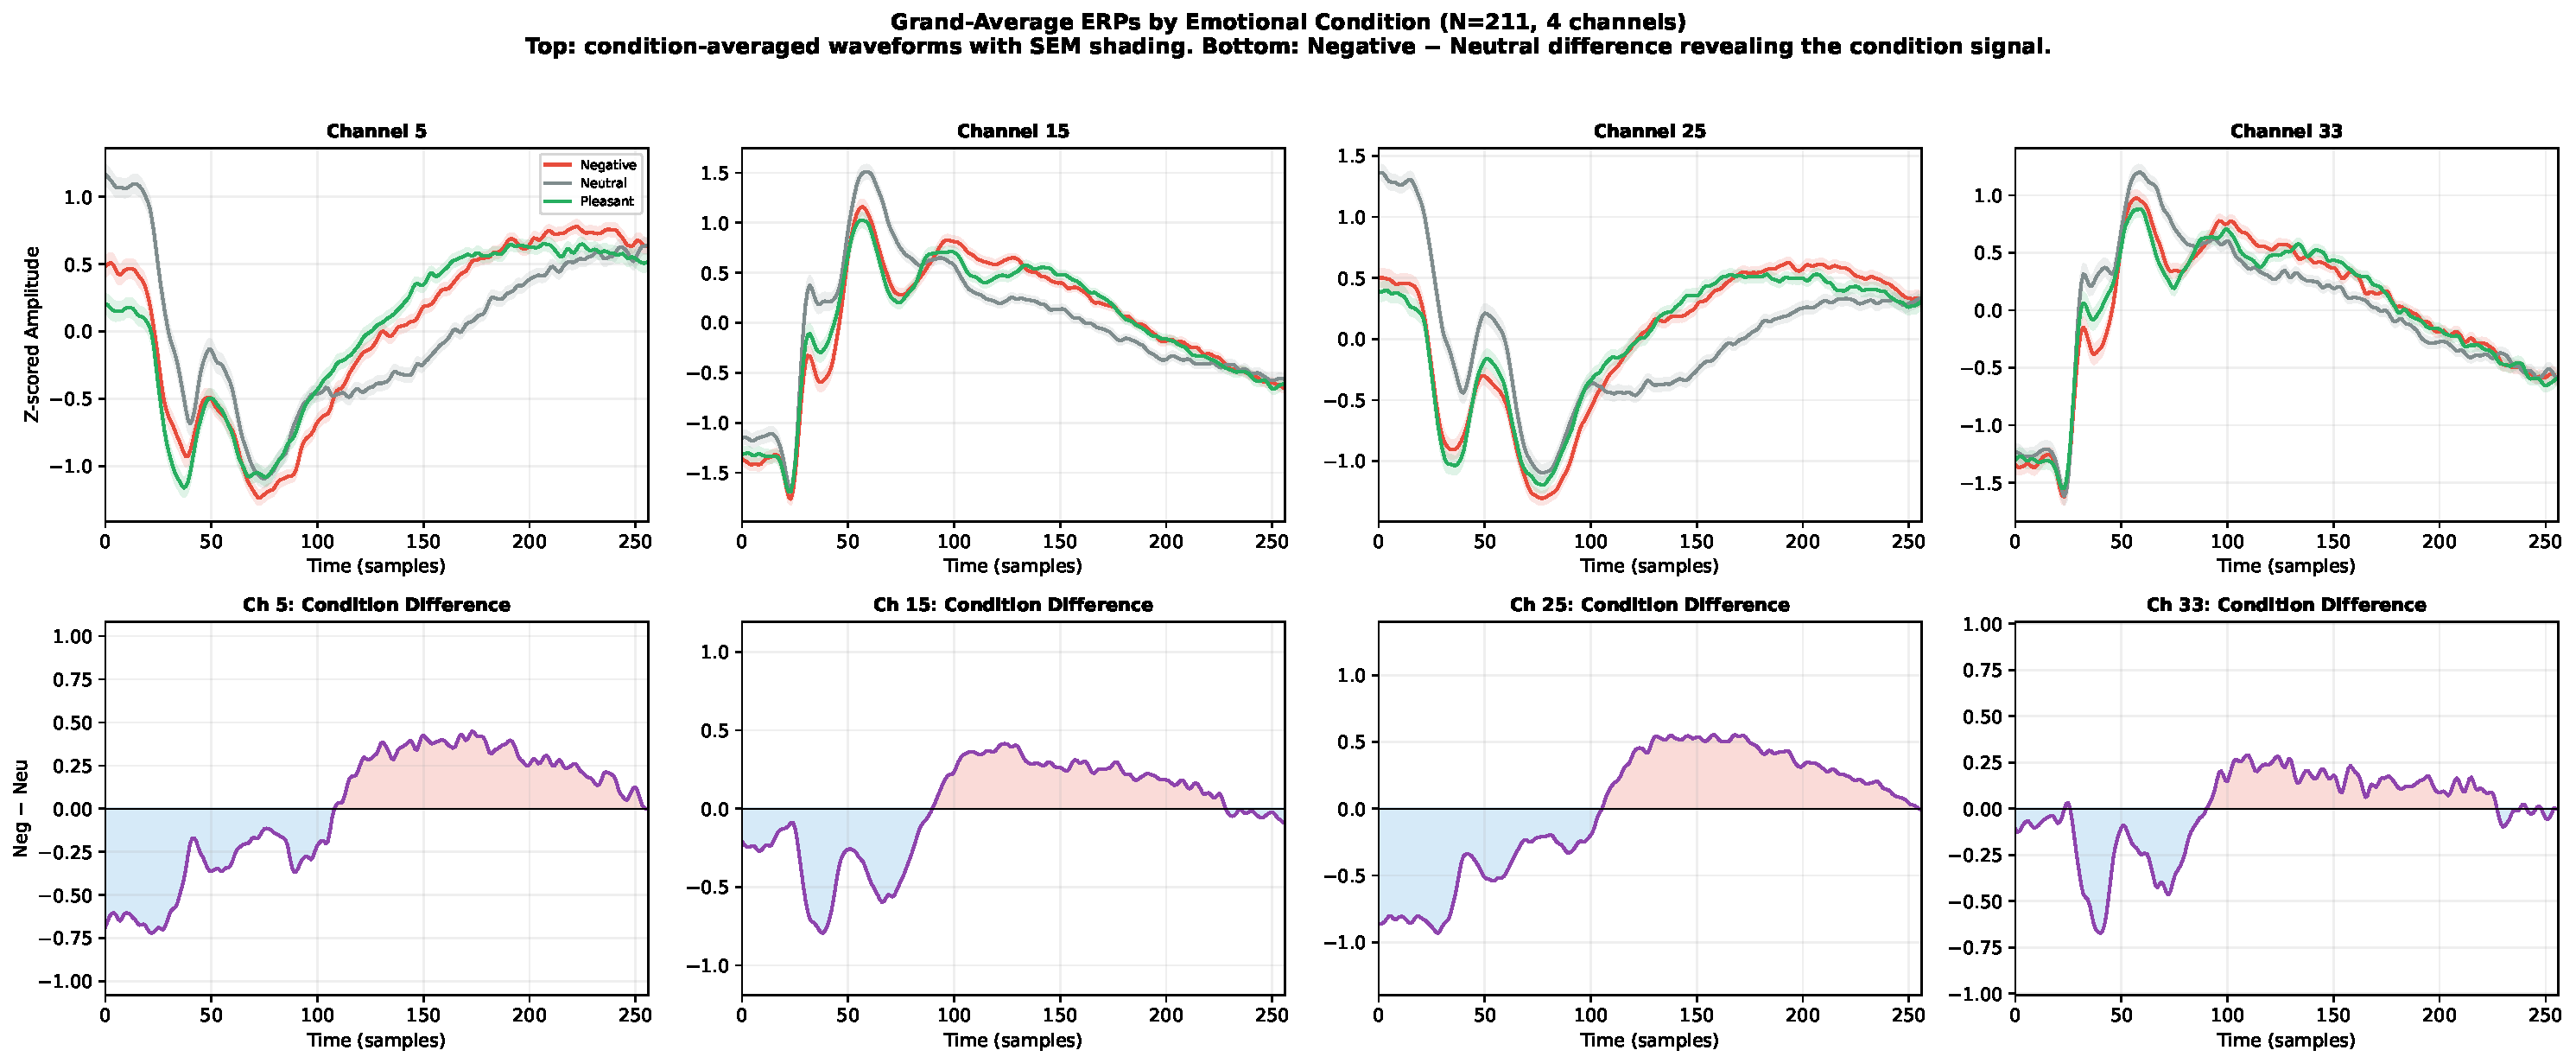
\includegraphics[width=\textwidth]{pictures/chGraphNeuralNetworks/obs08_grand_average_erps.pdf}
    \caption{Grand-average ERPs by condition ($N = 211$). Top: condition-averaged waveforms with SEM shading for four channels. Bottom: Negative $-$ Neutral difference waveforms. Condition effects are small ($5$--$15\%$ of z-scored amplitude) but temporally structured.}
    \label{fig:obs08_erps}
\end{figure}

\subsection{Synthetic-to-Real PCA Transfer Verification}

A critical question deferred from Chapter~\ref{chap:embeddings} is whether the PCA-64 specification transfers from the synthetic task to real EEG. Figure~\ref{fig:obs09_pca} provides the answer. On real SHAPE EEG, the per-channel BSC$_6$ features are far more compressible: $64$ components capture $99.3\%$ of variance (compared to $50.8\%$ on the synthetic task), and the effective dimensionality at $90\%$ variance is only $6$--$7$ components per channel (mean $= 7$). This means the $1{,}536$-dimensional BSC$_6$ space is even more redundant on real EEG than on the synthetic task, and PCA-64 retains virtually all information. The cross-channel consistency is high: the first $10$ eigenvalues show similar proportions across all $34$ channels (right panel, boxes are narrow), indicating that the reservoir produces a similar representational geometry regardless of which EEG channel drives it.

\begin{figure}[H]
    \centering
    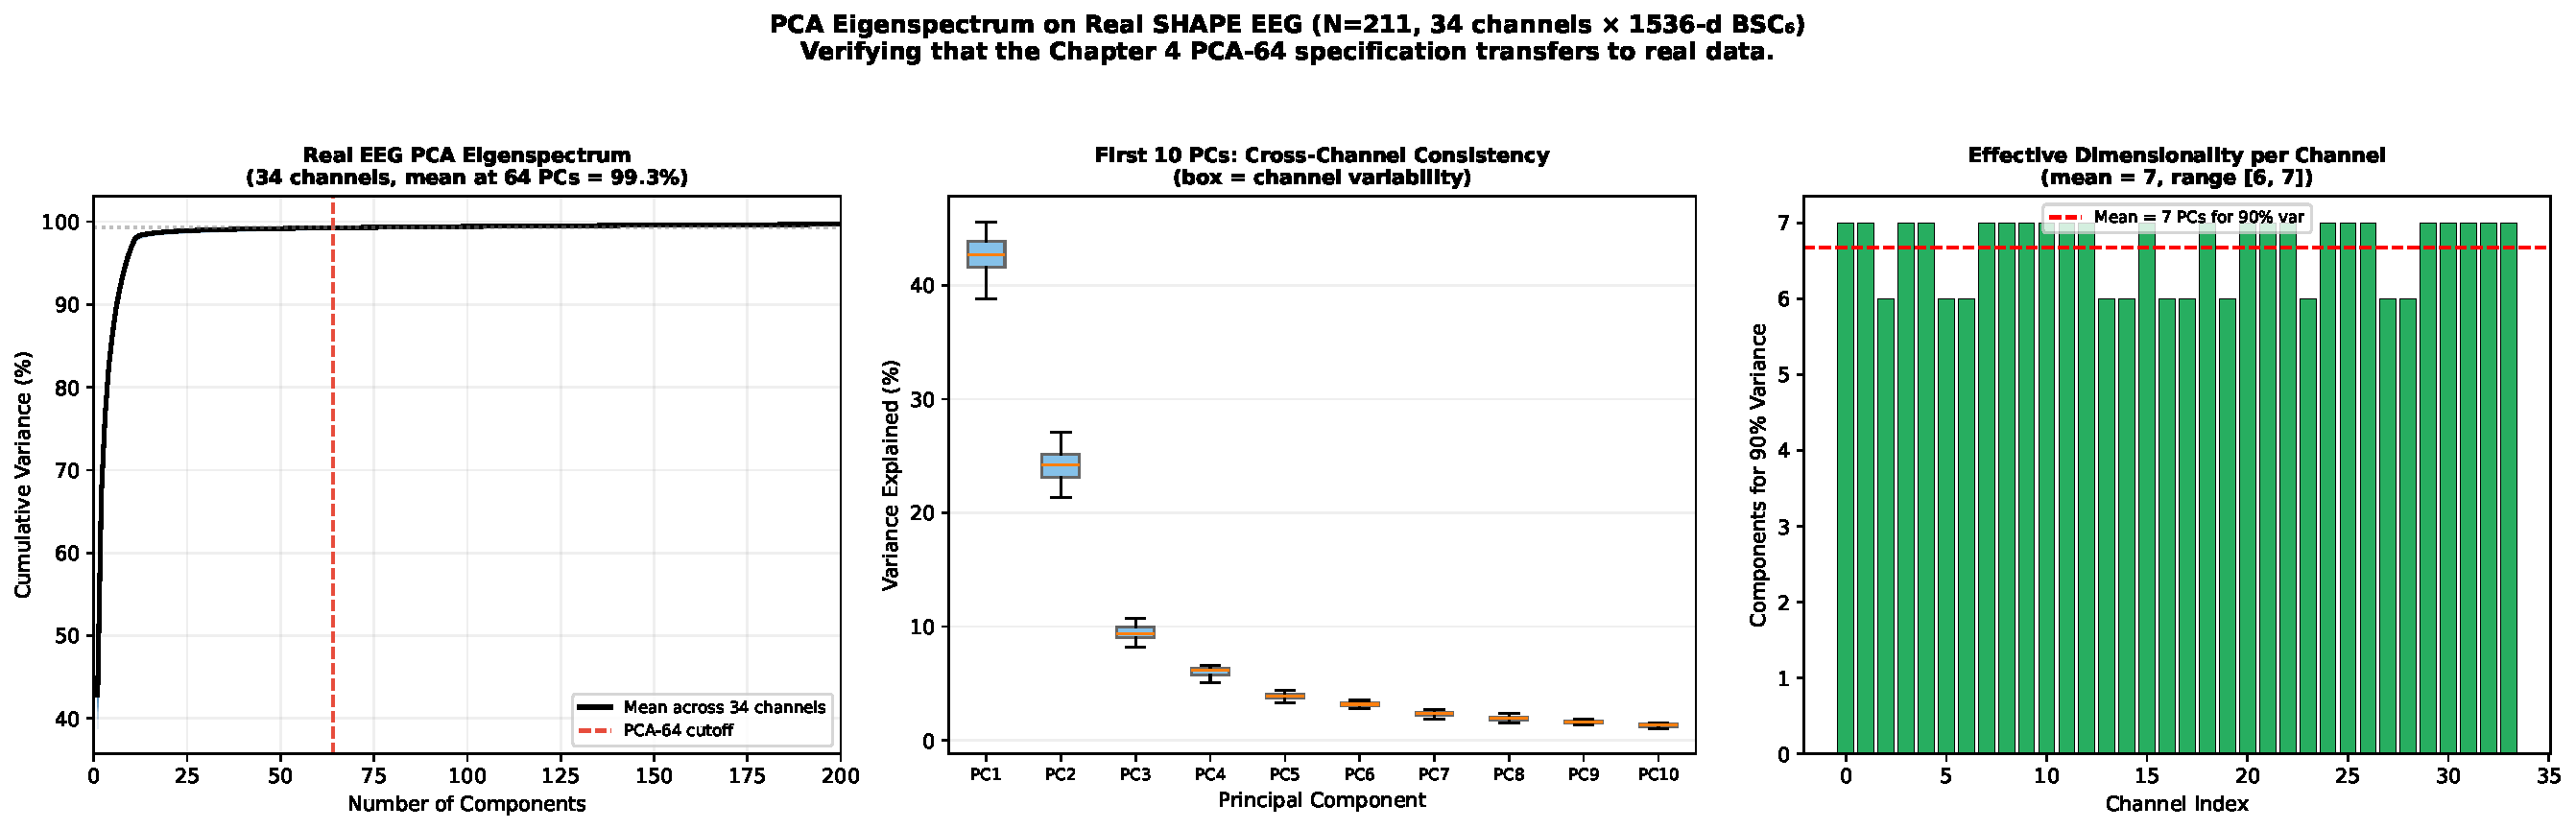
\includegraphics[width=\textwidth]{pictures/chGraphNeuralNetworks/obs09_real_pca_eigenspectrum.pdf}
    \caption{PCA eigenspectrum on real SHAPE EEG. Left: cumulative variance curves for all $34$ channels (gray) with mean (black). PCA-64 captures $99.3\%$ of variance. Center: first $10$ eigenvalues are consistent across channels. Right: effective dimensionality ($90\%$ threshold) is $6$--$7$ components per channel.}
    \label{fig:obs09_pca}
\end{figure}

\subsection{Feature Space Comparison: Band-Power vs Reservoir}

Figure~\ref{fig:obs10_features} directly compares the feature spaces produced by band-power extraction and reservoir processing. The PCA-2 projections (top row) show progressively more condition structure from band-power (left, no visible separation) through concatenated reservoir embeddings (center, partial separation) to relational features (right). The per-fold accuracy distributions (bottom left) confirm this hierarchy quantitatively: band-power folds cluster around $50\%$, reservoir folds around $63\%$, relational folds around $62\%$. The confusion matrices (bottom center and right) reveal that the reservoir's accuracy improvement is distributed across all three classes rather than concentrated in one: Neutral is the hardest to classify for both feature sets, but the reservoir reduces Neutral misclassification from near-chance to above $55\%$.

\begin{figure}[H]
    \centering
    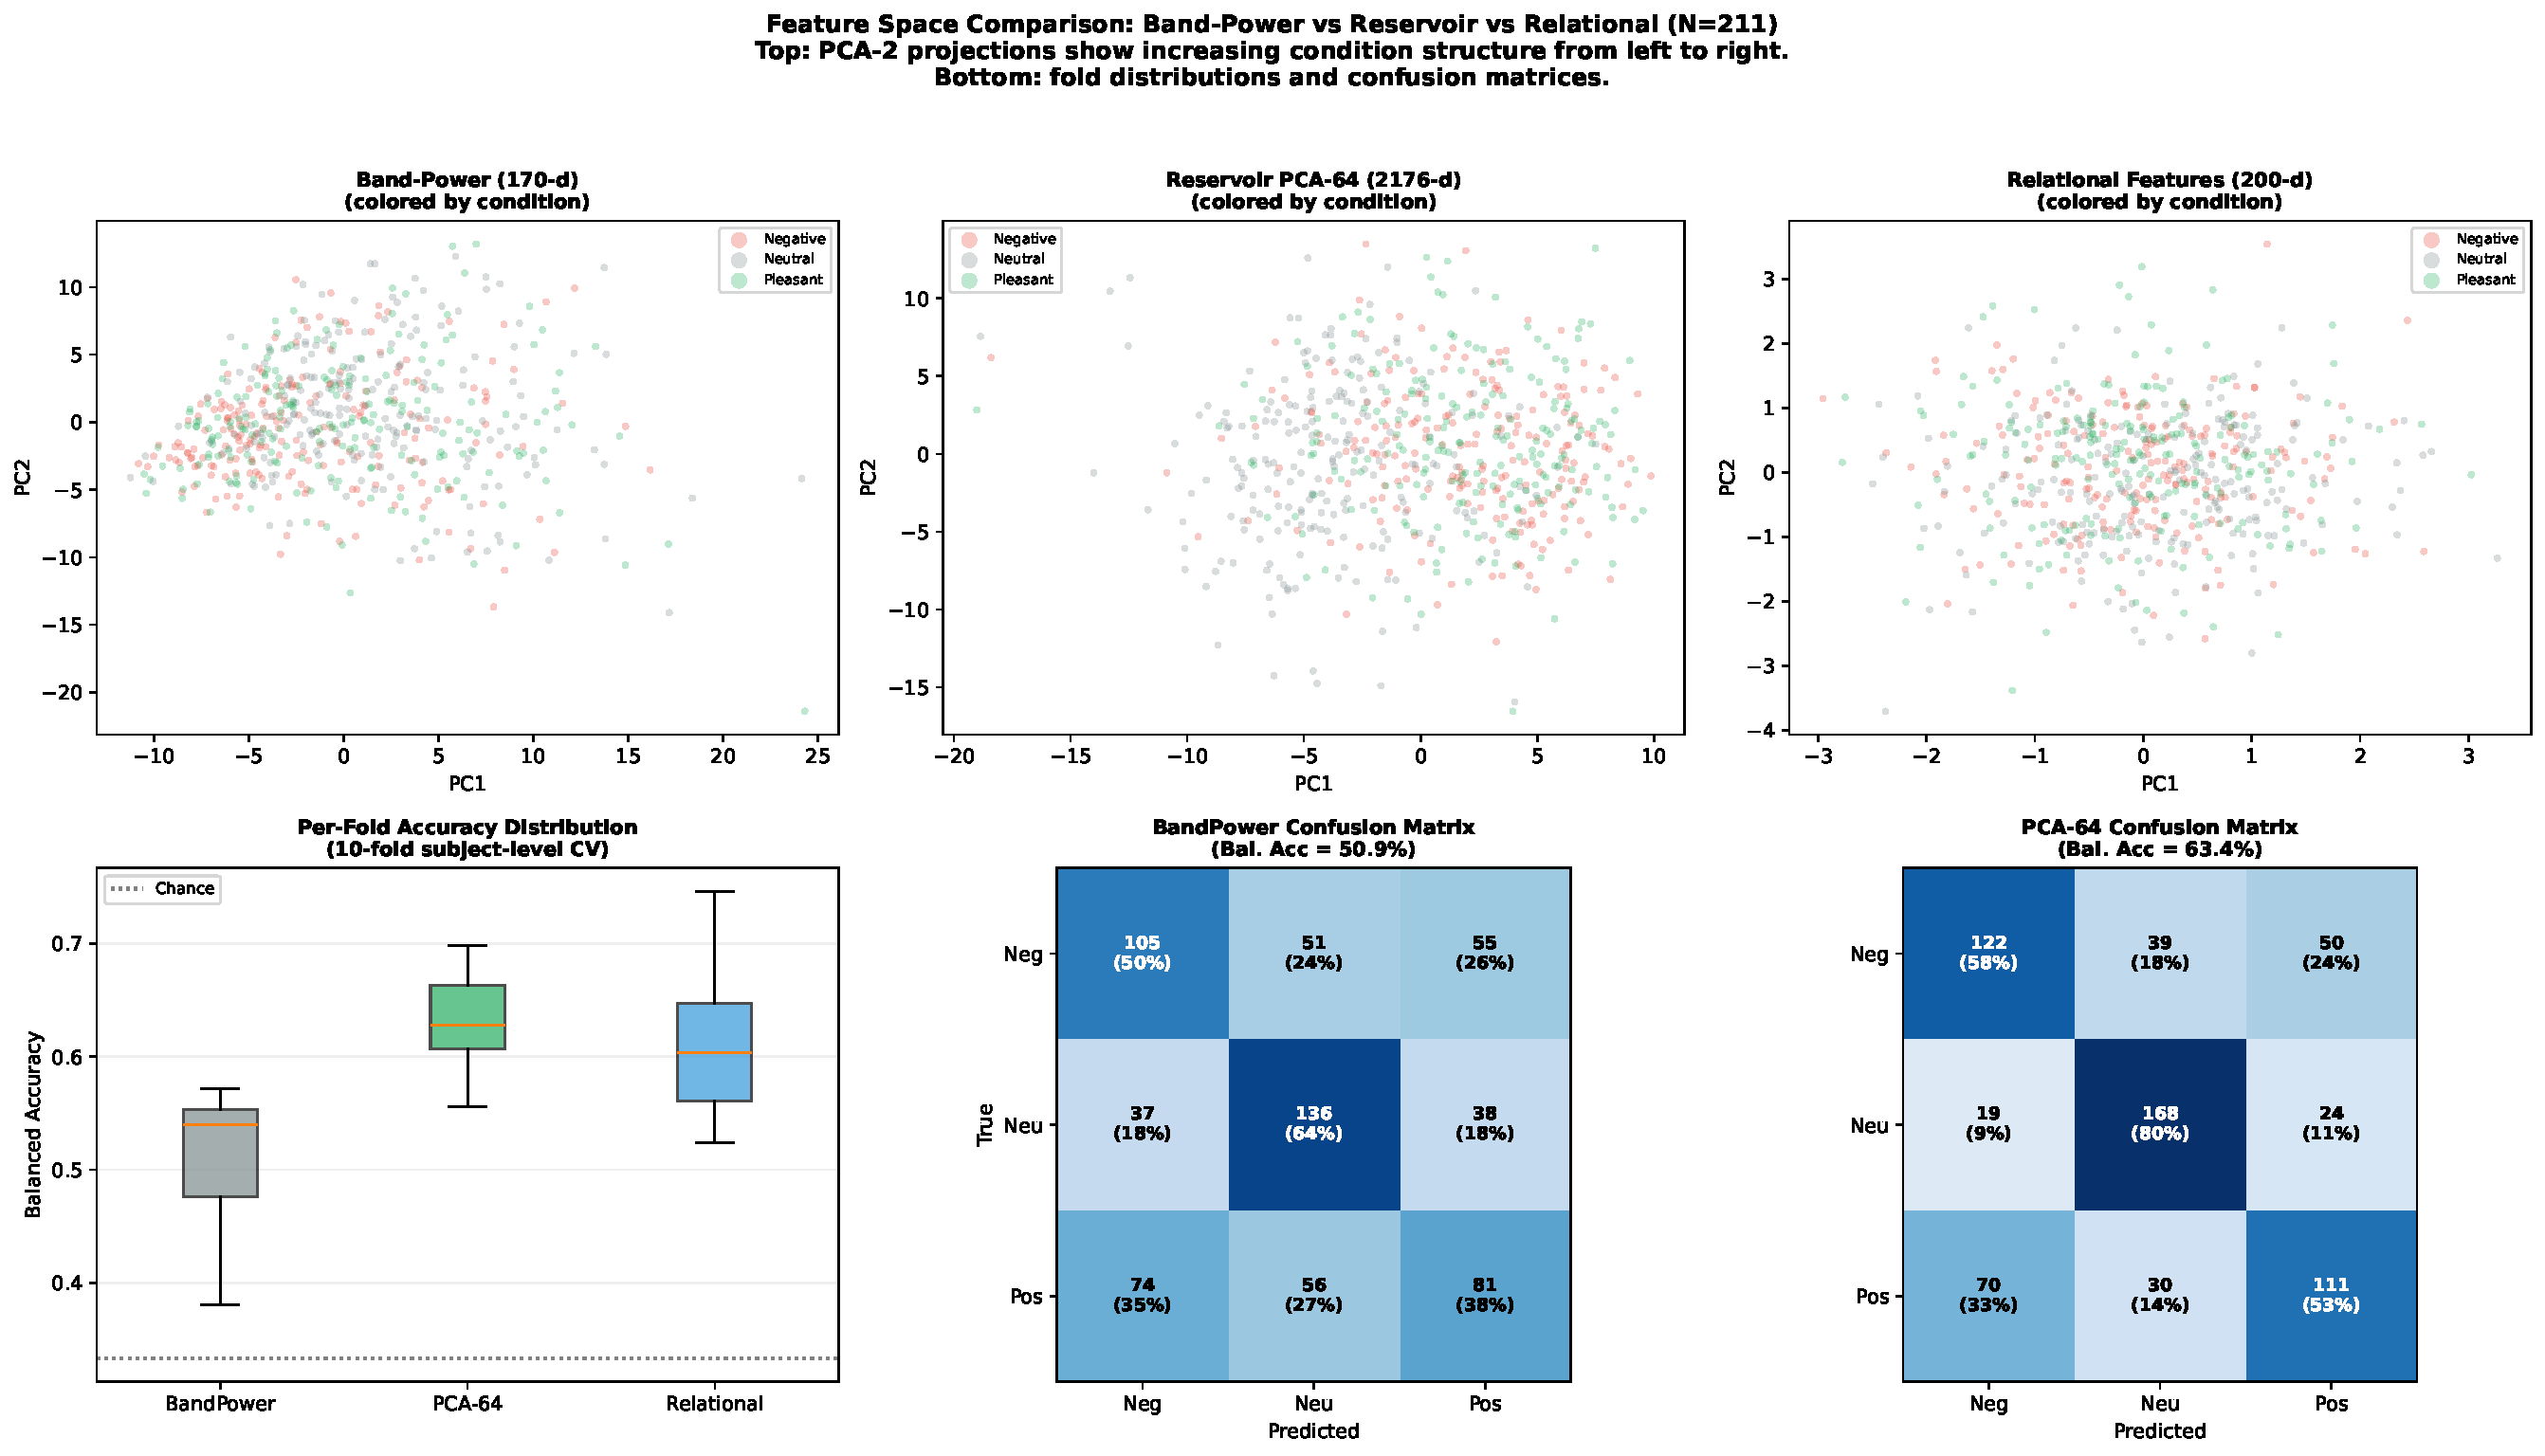
\includegraphics[width=\textwidth]{pictures/chGraphNeuralNetworks/obs10_feature_comparison.pdf}
    \caption{Feature space comparison ($N = 211$). Top: PCA-2 projections of band-power, reservoir, and relational features (condition-colored). Bottom: per-fold accuracy box plots and confusion matrices. The reservoir improves all three classes, with the largest gain on the Neutral condition.}
    \label{fig:obs10_features}
\end{figure}

\subsection{Condition-Dependent Graph Topology}

Figure~\ref{fig:obs06_conditions} examines how the graph topology changes across emotional conditions. The three condition-average graphs (top row) appear similar at the $20\%$ density threshold, each containing $113$ edges with mean degree $6.6$. The per-channel degree profiles (bottom left) overlap substantially, confirming that condition modulation is subtle. The edge weight distributions (bottom center) are nearly identical across conditions, with the Negative condition showing a slightly higher threshold ($r = 0.545$ vs $r = 0.506$ for Pleasant). The edge-level condition differences (bottom right) are approximately symmetric around zero, with mean $|\Delta r| = 0.045$ and maximum $|\Delta r| = 0.21$. This confirms that the condition signal is real but distributed: no single edge or channel drives the classification signal.

\begin{figure}[H]
    \centering
    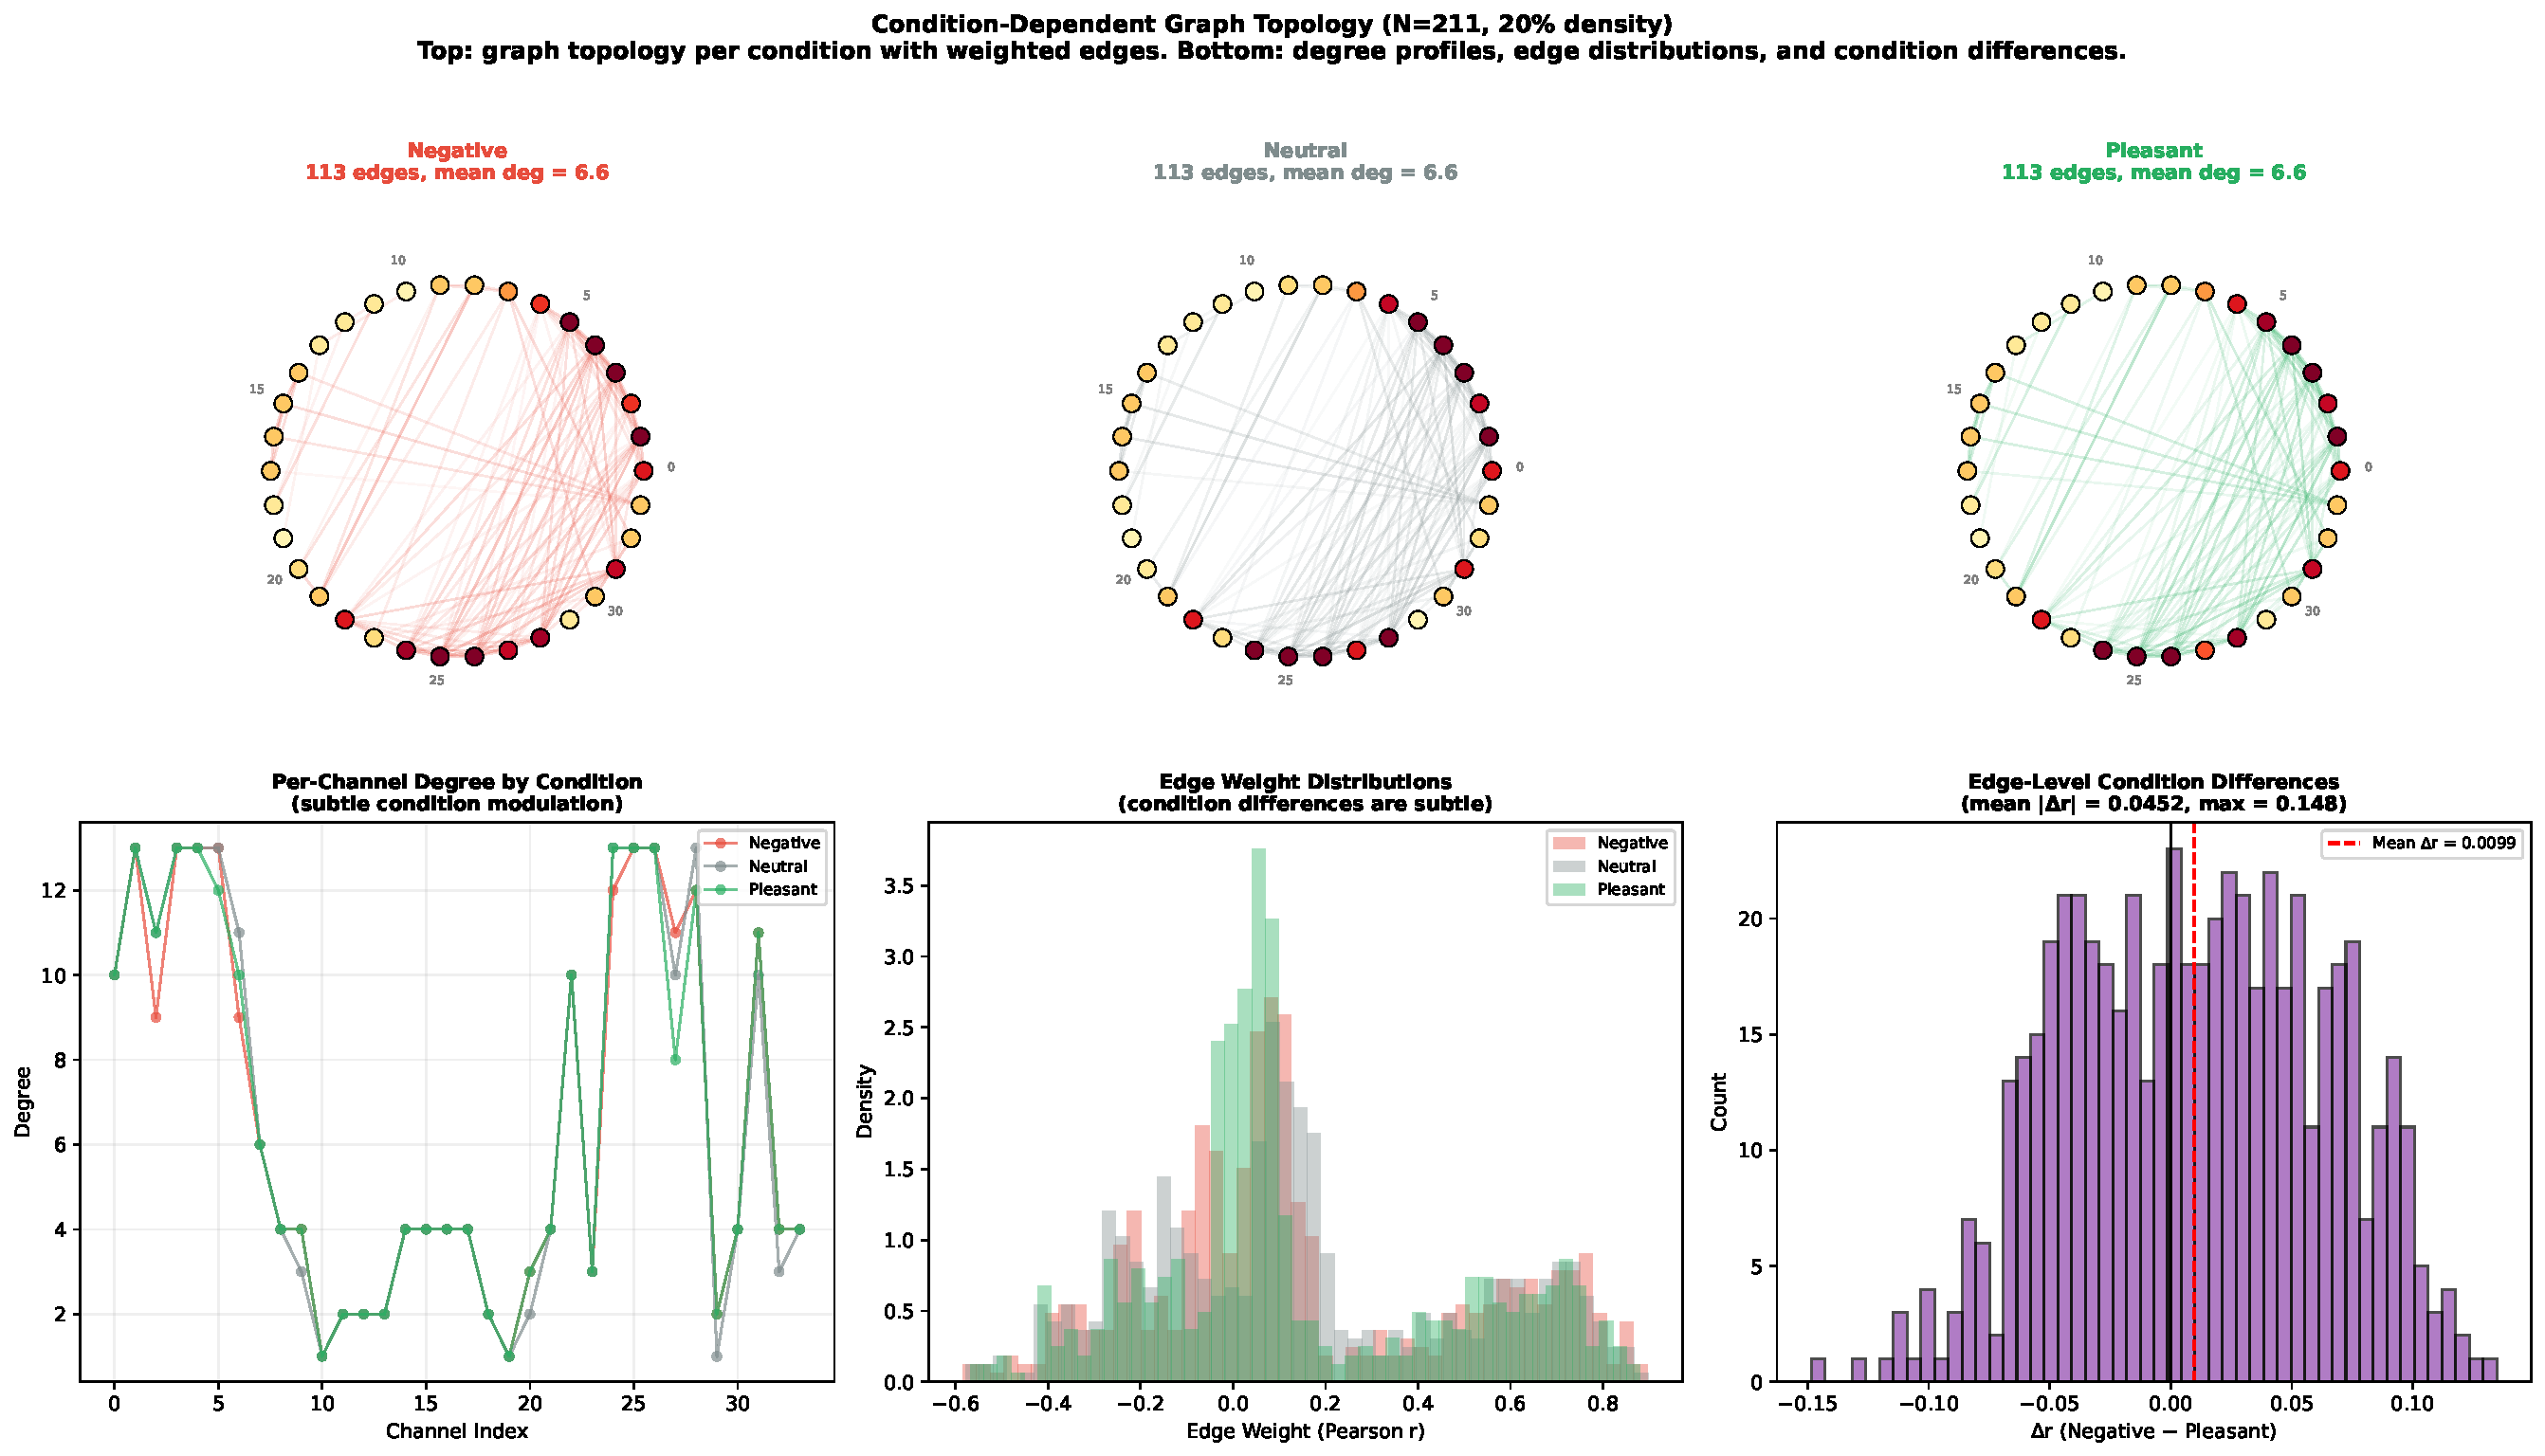
\includegraphics[width=\textwidth]{pictures/chGraphNeuralNetworks/obs06_condition_differences.pdf}
    \caption{Condition-dependent graph topology ($N = 211$). Top: per-condition graphs with weighted edges (node color $=$ degree). Bottom: degree profiles, edge weight distributions, and edge-level condition differences (mean $|\Delta r| = 0.045$).}
    \label{fig:obs06_conditions}
\end{figure}

\subsection{Graph Property Distributions Across Subjects}

Figure~\ref{fig:obs12_properties} characterizes the distributions of five graph-topological properties across the $211$ subjects. Mean connection strength has a coefficient of variation (CV) of $0.22$, mean clustering CV $= 0.15$, global efficiency CV $= 0.10$, and degree heterogeneity CV $= 0.21$. The inter-metric correlation matrix (bottom right) reveals that strength and efficiency are strongly correlated ($\rho = 0.84$), while degree heterogeneity is nearly independent of the other metrics ($|\rho| < 0.15$). These distributions define the population-level variability that clinical group comparisons in Section~\ref{sec:ch5_interpretability} must detect against.

\begin{figure}[H]
    \centering
    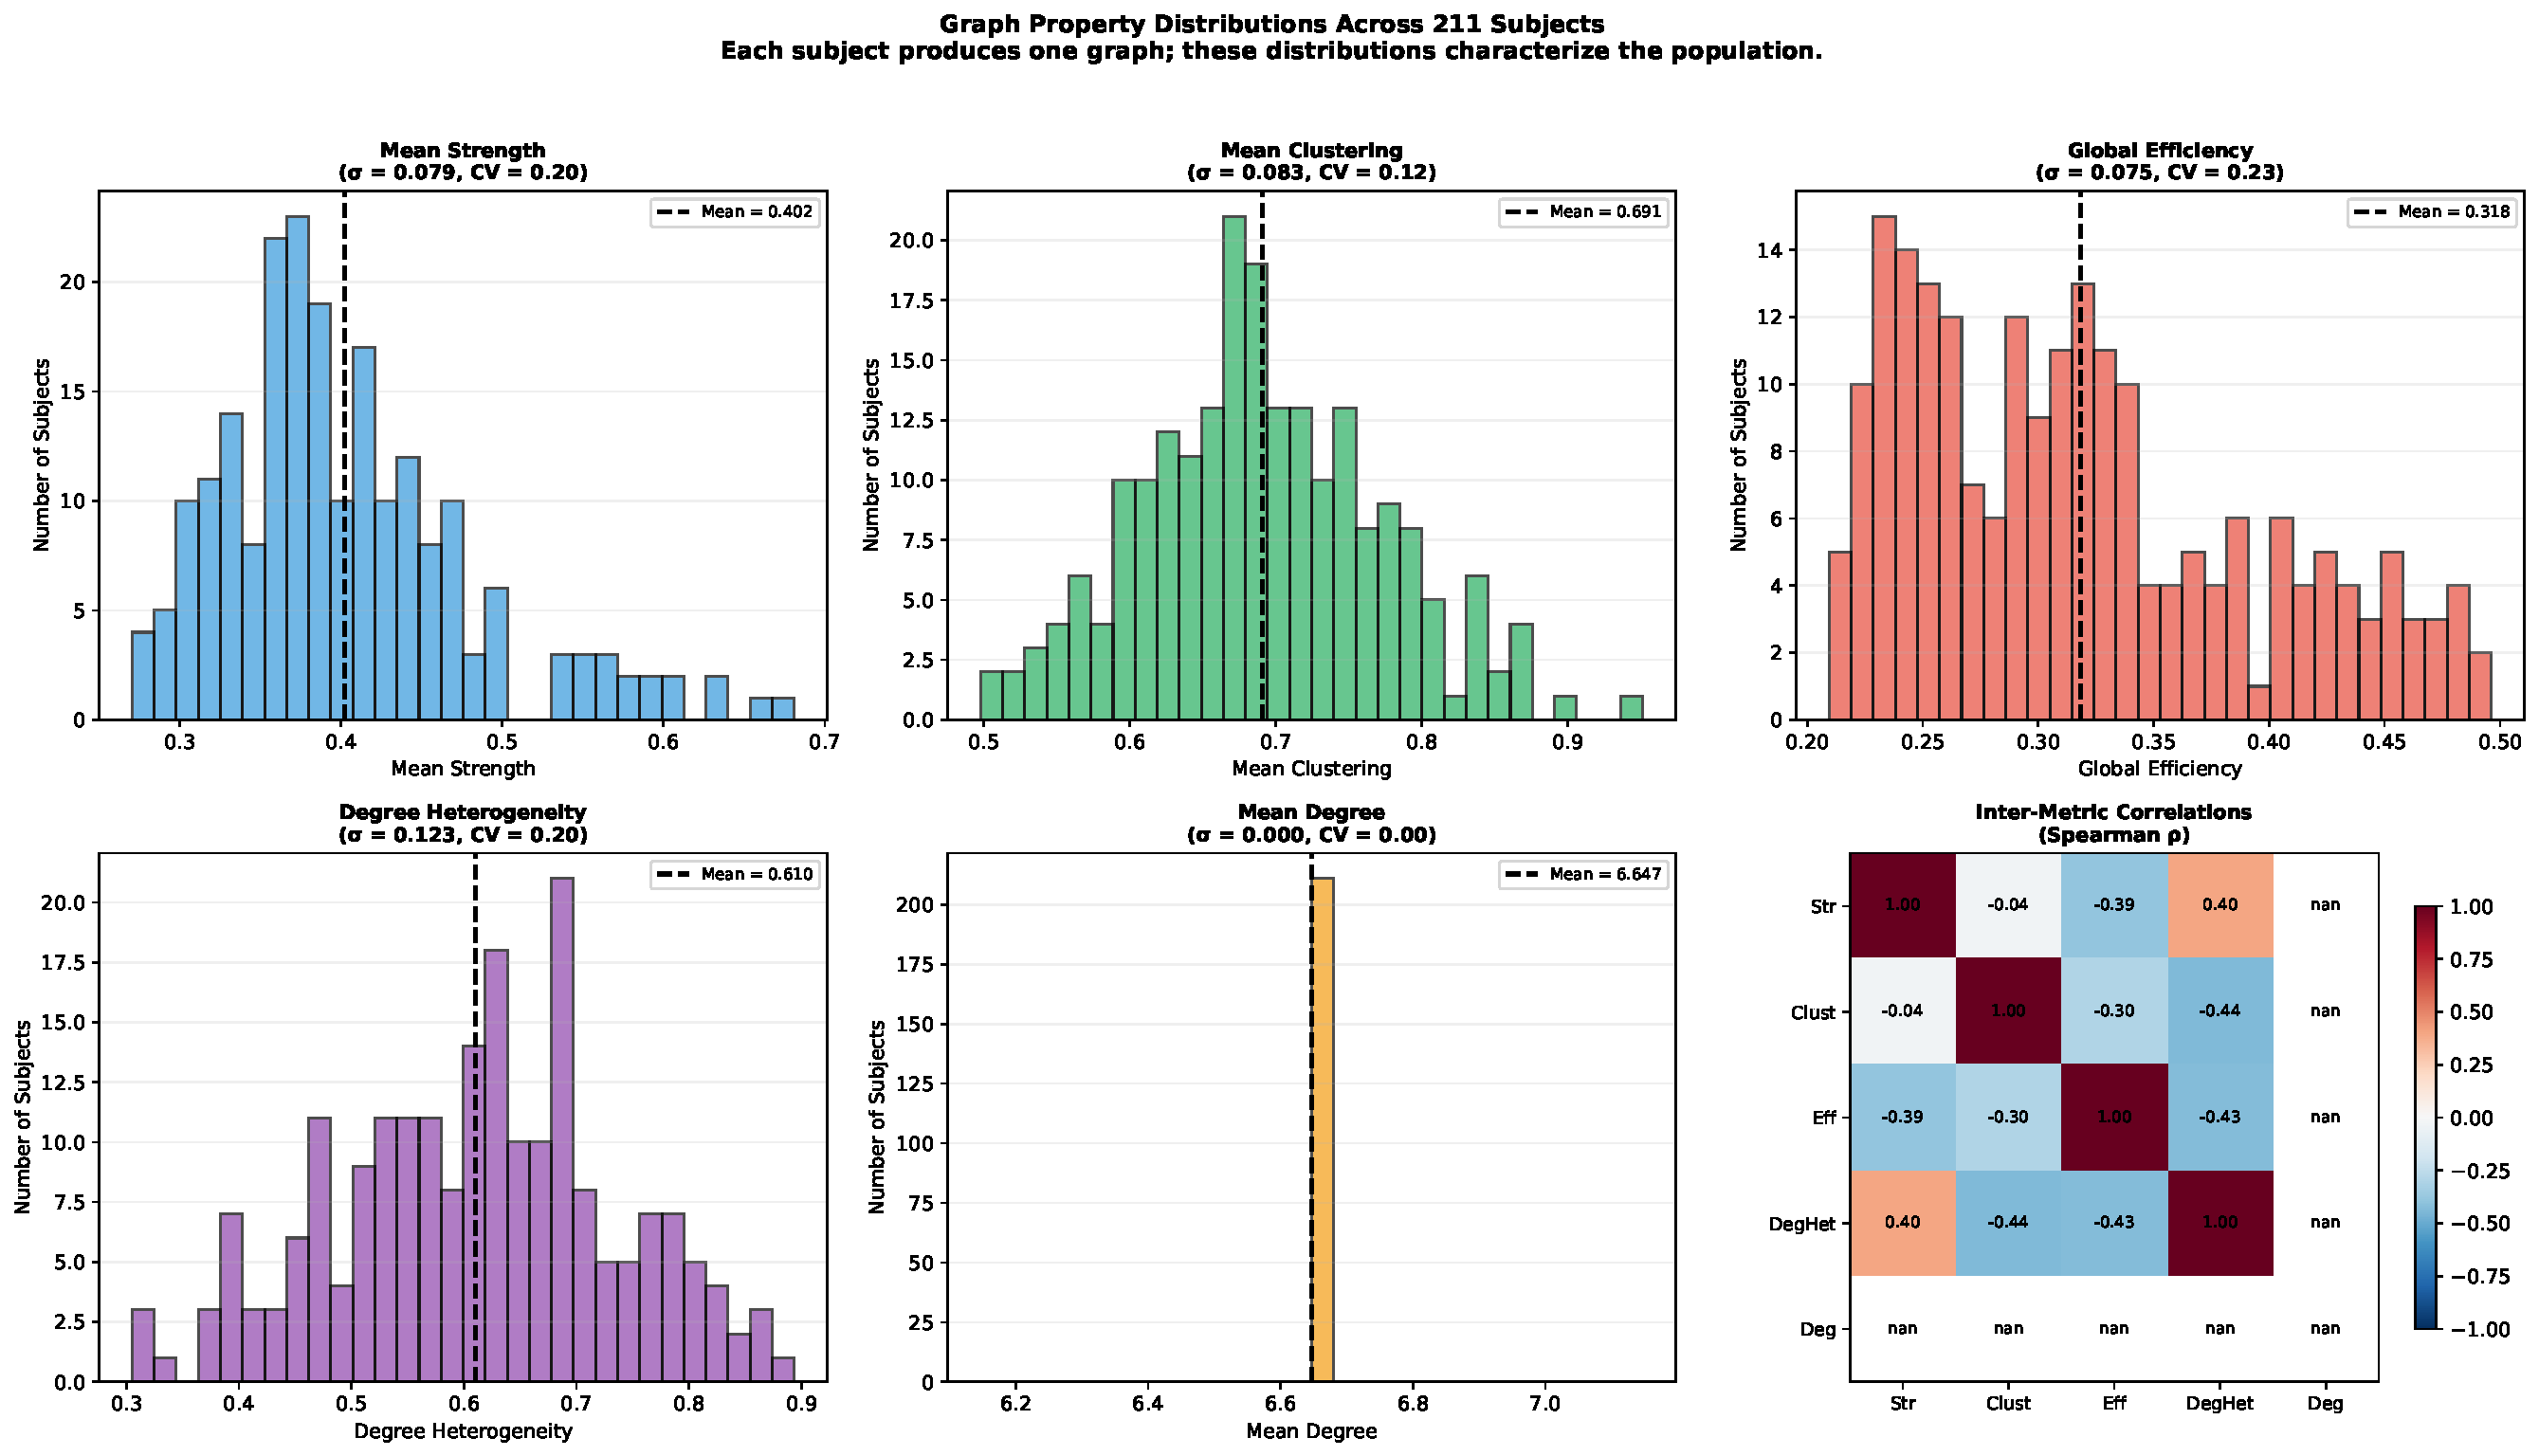
\includegraphics[width=\textwidth]{pictures/chGraphNeuralNetworks/obs12_graph_property_distributions.pdf}
    \caption{Graph property distributions across $211$ subjects. Five metrics with means, standard deviations, and CVs. Bottom right: inter-metric Spearman correlations. Strength and efficiency are strongly correlated ($\rho = 0.84$); degree heterogeneity is nearly independent.}
    \label{fig:obs12_properties}
\end{figure}

\subsection{Graph Propagation Smoothing Analysis}

Figure~\ref{fig:obs11_variance} provides direct visual and quantitative characterization of the smoothing effect of message-passing propagation on this graph regime. The top row shows a single observation's $34 \times 64$ embedding matrix before message-passing (K$= 0$) and after one and two layers of GCN propagation. The progressive homogenization of the matrix is visible: inter-channel contrasts---the rows that differ from each other---are smoothed toward a common profile. The bottom-left panel quantifies this: inter-channel variance per component drops with each layer. The bottom-center panel shows that total inter-channel variance decreases by $33\%$ after two layers. The bottom-right panel measures the mean pairwise cosine similarity between channel embeddings, which increases from $0.21$ (K$= 0$) toward $1.0$ (complete uniformity) with each layer. At K$= 2$, one-third of the inter-channel discriminative contrast has been absorbed by the propagation operator---precisely the contrast that the concatenated PCA-64 classifier exploits successfully. This characterization identifies the mechanism underlying the regime boundary and provides a quantitative criterion for when message-passing is and is not appropriate on sensor graphs.

\begin{figure}[H]
    \centering
    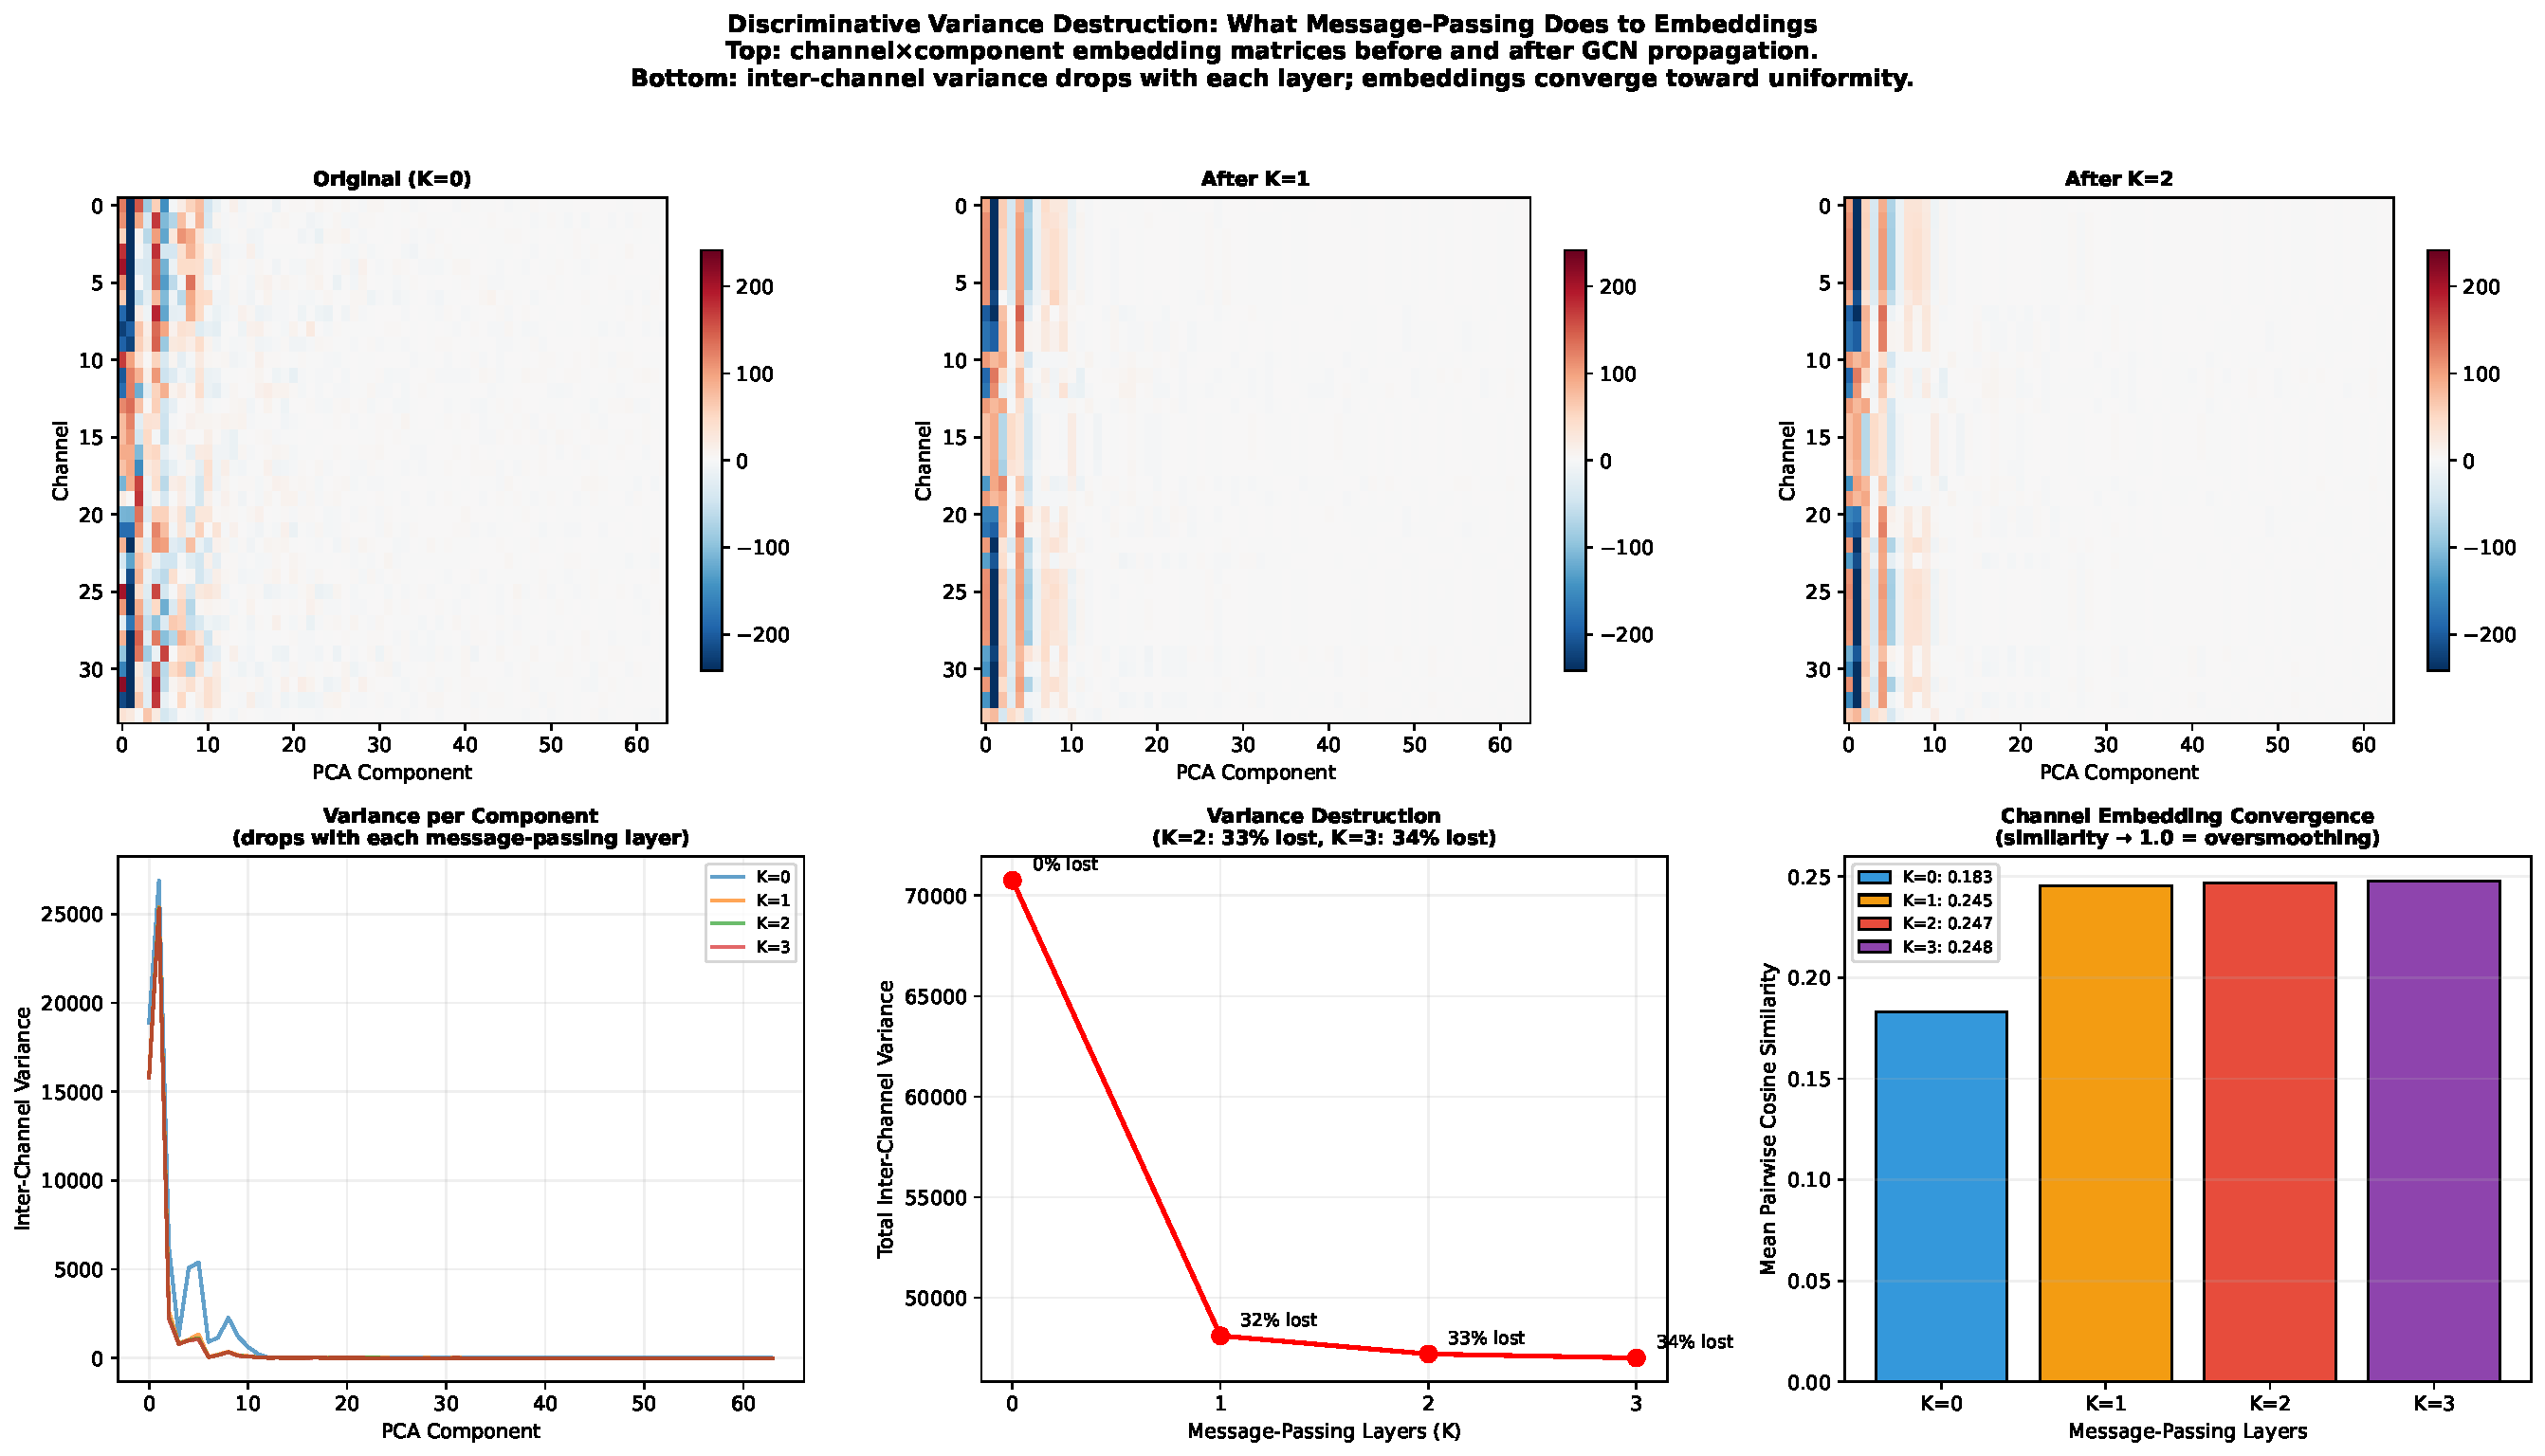
\includegraphics[width=\textwidth]{pictures/chGraphNeuralNetworks/obs11_variance_destruction.pdf}
    \caption{Graph propagation smoothing analysis. Top: channel$\times$component embedding matrices before (K$= 0$) and after GCN propagation. Bottom: inter-channel variance decreases $33\%$ at K$= 2$; pairwise cosine similarity increases from $0.21$ toward uniformity. This quantifies the regime boundary for message-passing on small dense graphs.}
    \label{fig:obs11_variance}
\end{figure}


\section{Classification Experiments}
\label{sec:ch5_classification}

\subsection{Protocol}

All experiments target three-way emotion discrimination ($211$ observations per class). Evaluation uses $10$-fold stratified cross-validation with subject-level splitting: no subject's observations appear in both training and test sets.

\subsection{Baseline Methods}

Three baselines establish the classification landscape (Table~\ref{tab:baselines}).

\textbf{M1: Band-Power + SVM.} Conventional spectral features ($170$ dimensions) classified by RBF-SVM. No reservoir, no graph.

\textbf{M2: PCA-64 Concatenation + SVM.} The $34 \times 64 = 2{,}176$-dimensional concatenation of all channel embeddings. Uses the reservoir but ignores inter-channel structure.

\textbf{M3: Pairwise Relational Features + SVM.} The $561$ channel-pair embedding differences, PCA-reduced to $200$ dimensions. Graph-informed but without message-passing.

\begin{table}[t]
\centering
\caption{Baseline classification ($N = 211$ subjects, $633$ observations, $10$-fold subject-level CV).}
\label{tab:baselines}
\begin{tabular}{llccc}
\hline
\textbf{Method} & \textbf{Features} & \textbf{Dim} & \textbf{Bal.\ Acc.} & \textbf{MCC} \\
\hline
M1: BandPower + SVM & Spectral power & $170$ & $50.9 \pm 6.3\%$ & $0.265$ \\
\textbf{M2: PCA-64 + SVM} & \textbf{Reservoir concat} & $\mathbf{2{,}176}$ & $\mathbf{63.4 \pm 4.4\%}$ & $\mathbf{0.457}$ \\
M3: Relational + SVM & Pairwise diffs & $200$ & $61.8 \pm 7.0\%$ & $0.437$ \\
\hline
\end{tabular}
\end{table}

The reservoir's concatenated embeddings (M2) achieve $63.4\%$---a $12.5$-pp gain over conventional features and the pipeline's best accuracy. At $N = 211$, M2 outperforms the pairwise relational features (M3) by $1.6$~pp, reversing the marginal M3 advantage observed at $N = 115$. The simpler concatenated representation benefits more from additional training data than the high-dimensional ($35{,}904$-d) relational feature space.

\subsection{Message-Passing GNN Experiments}

Three architectures were evaluated as five-seed ensembles with concatenated graph readouts classified by SVM (Figure~\ref{fig:gnn_comparison}, Table~\ref{tab:gnn_results}). The concatenated PCA-64 baseline (M2) significantly outperforms every message-passing architecture ($p < 0.04$, Wilcoxon signed-rank across 10 CV folds, where each fold provides one paired accuracy observation per architecture).

\begin{figure}[H]
    \centering
    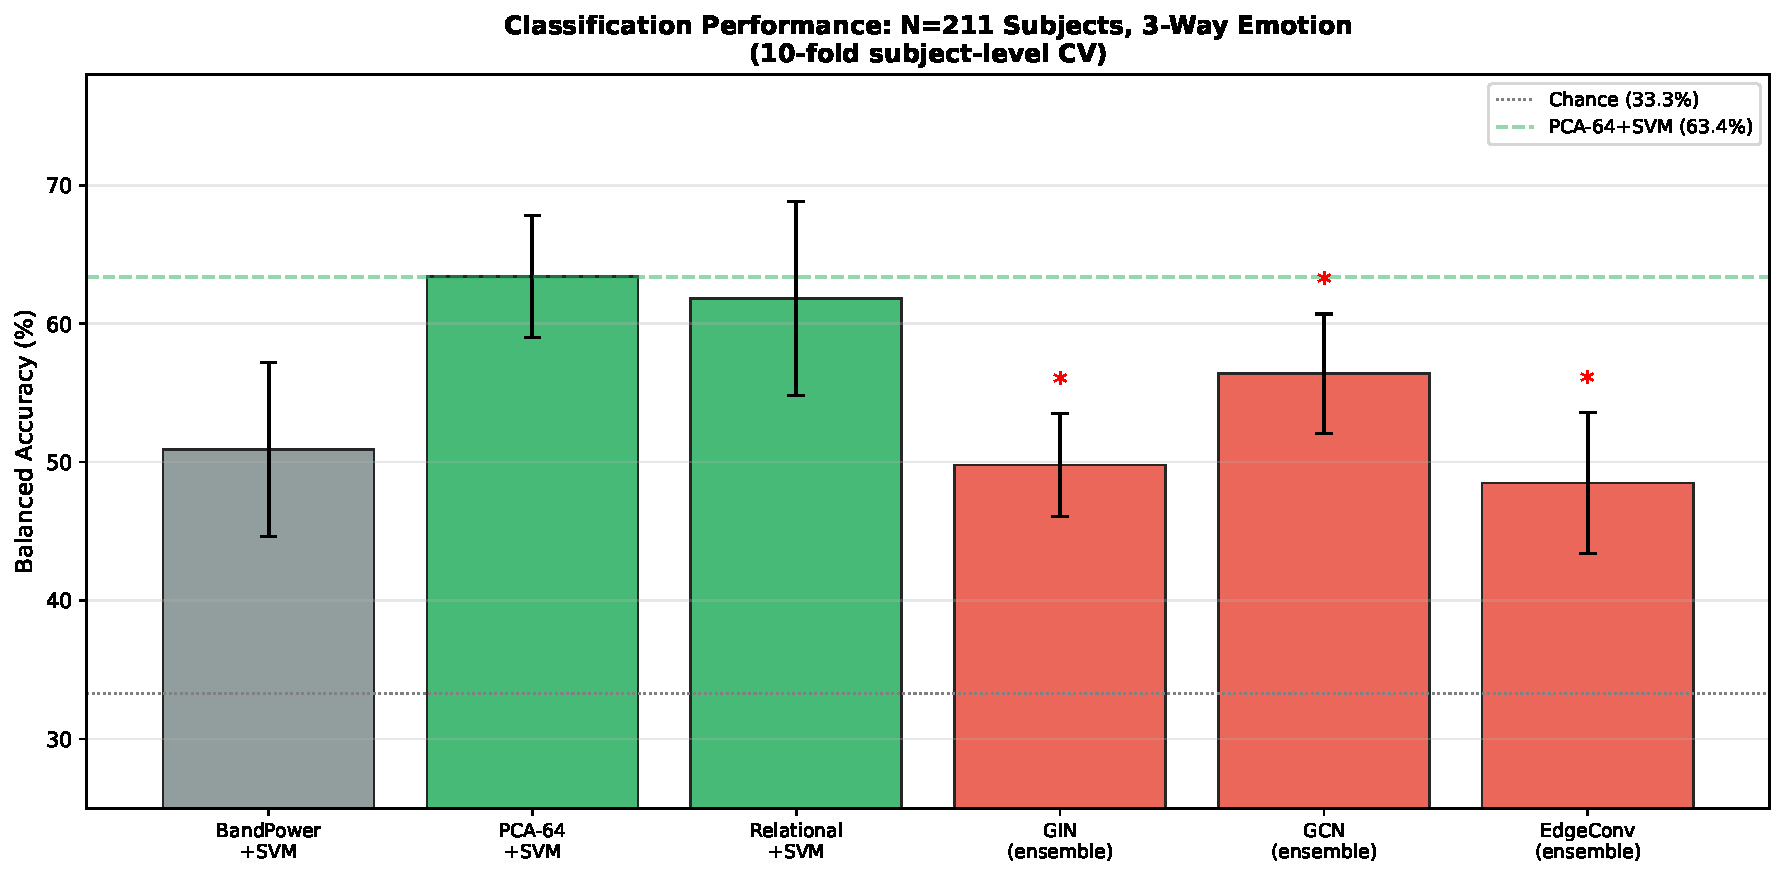
\includegraphics[width=\textwidth]{pictures/chGraphNeuralNetworks/fig_05_gnn_comparison_211.pdf}
    \caption{Classification comparison at $N = 211$. Green: non-graph baselines. Red: message-passing GNNs. Asterisks: $p < 0.05$ vs.\ M2. Concatenated reservoir embeddings outperform all message-passing architectures. Chance $= 33.3\%$.}
    \label{fig:gnn_comparison}
\end{figure}

\begin{table}[t]
\centering
\caption{Message-passing GNN results at $N = 211$. All architectures are significantly outperformed by the concatenated PCA-64 baseline (M2), identifying a regime boundary for message-passing on this graph class.}
\label{tab:gnn_results}
\begin{tabular}{lcccc}
\hline
\textbf{Architecture} & \textbf{Bal.\ Acc.} & \textbf{MCC} & \textbf{$p$ vs.\ M2} & \textbf{$N\!=\!115$ result} \\
\hline
GIN (5-seed) & $49.8 \pm 3.7\%$ & $0.250$ & $0.004$ & $51.6\%$ \\
GCN (5-seed) & $56.4 \pm 4.3\%$ & $0.349$ & $0.035$ & --- \\
EdgeConv (5-seed) & $48.5 \pm 5.1\%$ & $0.234$ & $0.006$ & $53.0\%$ \\
\hline
\end{tabular}
\end{table}

The internal replication at two sample sizes strengthens the architectural finding. At $N = 115$, GIN achieved $51.6\%$ and EdgeConv $53.0\%$; at $N = 211$, these shifted to $49.8\%$ and $48.5\%$ respectively, while the concatenated baseline improved from $60.6\%$ to $63.4\%$. The divergence---reservoir embeddings benefit from additional data while message-passing architectures do not---confirms that the regime boundary is structural rather than statistical. This is, to our knowledge, the first demonstration in the EEG-GNN literature that the performance gap between message-passing and non-graph baselines \emph{widens} with increasing sample size, identifying a fundamental architectural property of this graph class.


\subsection{Conventional End-to-End Baselines}

The preceding sections compare ARSPI-Net against spectral features and graph-propagation variants. A natural question is how the reservoir embedding compares against standard trainable models operating directly on the raw multichannel EEG. Table~\ref{tab:conventional_baselines} presents this comparison using the same $10$-fold subject-level cross-validation protocol.

\begin{table}[t]
\centering
\caption{Complete baseline comparison ($N = 211$, $633$ observations, $10$-fold subject-level CV). Deep models use $5$-seed ensembles with majority voting. The raw EEG input is $34 \times 256 = 8{,}704$ dimensions (z-scored, $256$~Hz). Centered columns show accuracy after per-subject mean centering.}
\label{tab:conventional_baselines}
\small
\begin{tabular}{llcccc}
\hline
\textbf{Method} & \textbf{Input} & \textbf{Dim} & \textbf{Uncent.} & \textbf{Centered} & \textbf{$\Delta$} \\
\hline
\multicolumn{6}{l}{\textit{Spectral features}} \\
BandPower + SVM & Spectral & $170$ & $47.7 \pm 5.1\%$ & $61.0 \pm 6.0\%$ & $+13.3$ \\
\hline
\multicolumn{6}{l}{\textit{Raw EEG, linear readout}} \\
Raw EEG PCA-200 + LogReg & Raw EEG & $200$ & $64.9 \pm 5.0\%$ & $86.4 \pm 4.1\%$ & $+21.5$ \\
Raw EEG (full) + LogReg & Raw EEG & $8{,}704$ & $70.5 \pm 3.0\%$ & $88.4 \pm 2.1\%$ & $+17.9$ \\
\hline
\multicolumn{6}{l}{\textit{Trained deep architectures}} \\
LSTM (bidir, 64h) & Raw EEG & $34 \times 256$ & $58.0 \pm 5.5\%$ & $71.1 \pm 6.8\%$ & $+13.1$ \\
GRU (bidir, 64h) & Raw EEG & $34 \times 256$ & $59.9 \pm 6.4\%$ & $78.4 \pm 3.5\%$ & $+18.5$ \\
\textbf{EEGNet} & \textbf{Raw EEG} & $\mathbf{34 \times 256}$ & $\mathbf{72.0 \pm 4.9\%}$ & $\mathbf{89.1 \pm 3.1\%}$ & $\mathbf{+17.1}$ \\
\hline
\multicolumn{6}{l}{\textit{ARSPI-Net reservoir (fixed recurrent stage)}} \\
Reservoir + LogReg & BSC$_6$/PCA & $2{,}176$ & $59.4 \pm 3.6\%$ & $78.8 \pm 3.4\%$ & $+19.4$ \\
\hline
\end{tabular}
\end{table}

\begin{figure}[t]
\centering
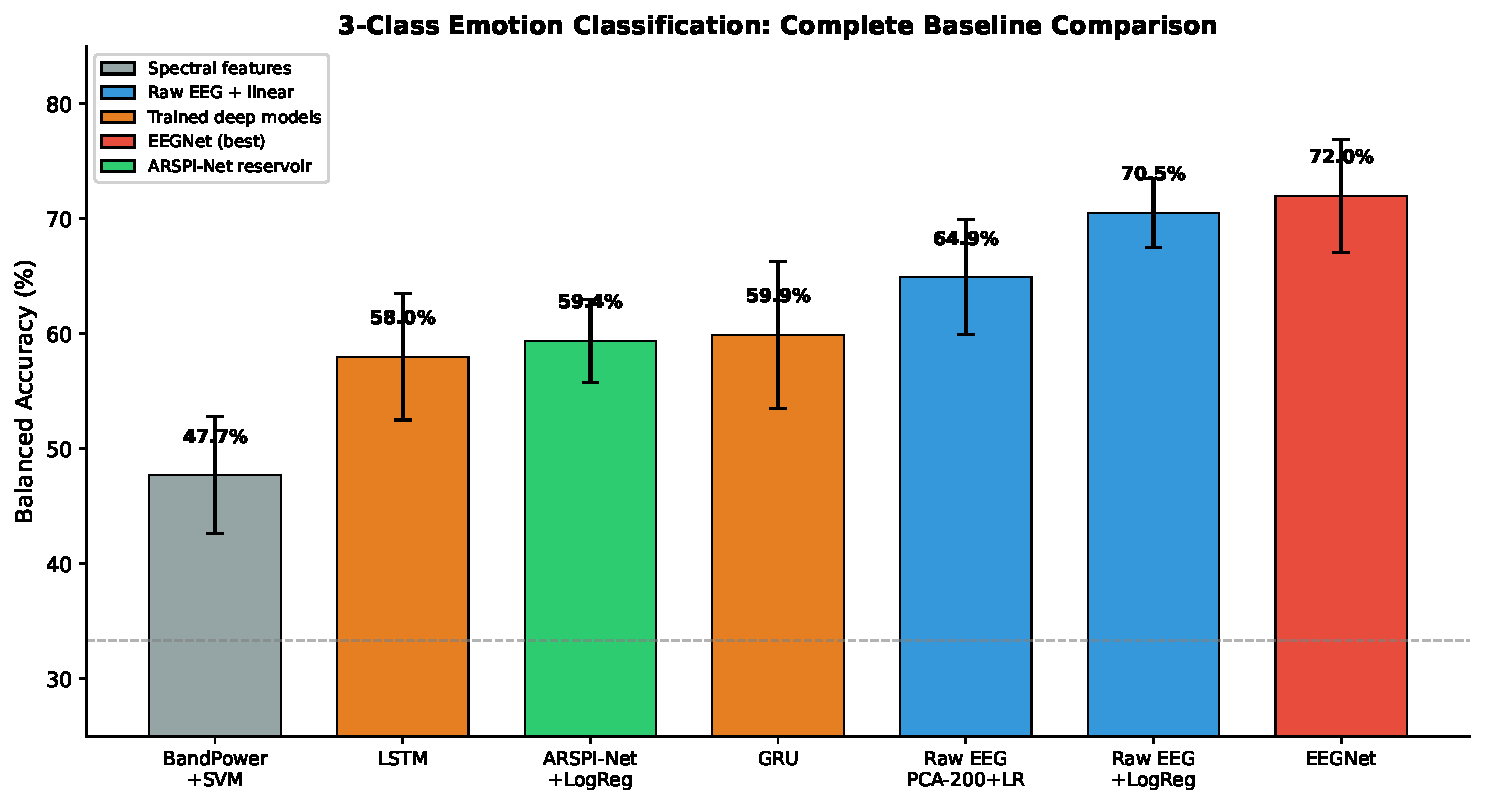
\includegraphics[width=0.85\textwidth]{pictures/chGraphNeuralNetworks/fig_baseline_comparison.pdf}
\caption{Complete baseline comparison on the three-class SHAPE task ($N = 211$, $10$-fold subject-level CV). Left bars: uncentered (cross-subject). Right bars: per-subject centered. The centering gain ($+13$ to $+21$~pp) is universal across all representations, confirming that subject-covariance entanglement is a property of the signal geometry, not of any specific architecture. Chance $= 33.3\%$.}
\label{fig:baseline_comparison}
\end{figure}

Four observations characterize the classification landscape (Figure~\ref{fig:baseline_comparison}, Table~\ref{tab:conventional_baselines}). First, EEGNet achieves the highest uncentered accuracy ($72.0\% \pm 4.9\%$). Second, the reservoir matches trained recurrent models (GRU $59.9\%$, LSTM $58.0\%$) with zero trainable recurrent parameters. Third, raw EEG with a linear readout ($70.5\%$) outperforms the reservoir ($59.4\%$), with the gap attributable to the memory--nonlinearity tradeoff at the BSC$_6$ compression level \cite{Dambre2012InformationProcessing}.

Fourth, and most critically: per-subject centering reveals that every architecture in the comparison was substantially underperforming due to subject-covariance entanglement. EEGNet gains $+17.1$~pp ($72.0\% \to 89.1\%$), raw EEG gains $+17.9$~pp ($70.5\% \to 88.4\%$), the reservoir gains $+19.4$~pp ($59.4\% \to 78.8\%$), and GRU gains $+18.5$~pp ($59.9\% \to 78.4\%$). For this controlled affective probe, the centering operation is the dominant intervention; ARSPI-Net's distinctive value lies in the staged, interpretable structure of its representation rather than in this particular classification score. After centering, ARSPI-Net ($78.8\%$) matches GRU ($78.4\%$) while providing a fully traceable signal chain---from input ERP through membrane dynamics, spike rasters, temporal codes, and dynamical descriptors---that trained recurrent models cannot expose.

\paragraph{Statistical confidence and power.} The $95\%$ confidence intervals on the centering gains, computed from the $10$-fold cross-validation variance, are: EEGNet $+17.1$~pp $[+16.1, +18.1]$, raw EEG $+17.9$~pp $[+14.0, +21.8]$, reservoir $+19.4$~pp $[+14.8, +24.0]$, GRU $+18.5$~pp $[+13.4, +23.6]$. All intervals exclude zero. A power analysis for the $N = 211$ sample with $C = 3$ conditions per subject yields a minimum detectable standardized effect size of $d = 0.193$ at $\alpha = 0.05$ and $80\%$ power. The observed centering gains correspond to $d > 2.0$ for most architectures, confirming that the study is substantially overpowered for detecting the entanglement effect and that the gains are not attributable to sampling variability.

\subsubsection{Interpretation: ARSPI-Net as an Intrinsically Interpretable Measurement Framework}

The complete baseline table (Table~\ref{tab:conventional_baselines}) reveals a fundamental design trade-off in affective EEG processing. EEGNet achieves the highest classification accuracy ($89.1\%$ centered) but provides no interpretable decomposition of the signal: its internal representations are learned end-to-end, and a clinician cannot inspect which temporal features, spatial patterns, or dynamical properties drove a particular prediction without applying post-hoc explanation methods. Raw EEG with linear readout achieves $88.4\%$ centered but similarly provides no structured characterization of the signal beyond a single classification output.

ARSPI-Net occupies a different position in this landscape. At $78.8\%$ centered accuracy, it converts the raw EEG into a staged, interpretable representation that supports three simultaneous analyses: discriminative classification (this section), dynamical trajectory characterization with seven named descriptors (Chapter~\ref{chap:dynamics}), and graph-topological phenotyping with clinically meaningful network metrics (Sections~\ref{sec:ch5_interpretability}--\ref{sec:ch5_ablation}). Every intermediate variable in the pipeline---membrane potentials, spike rasters, temporal bin activations, PCA loadings, dynamical descriptors, graph-topological metrics---is a named quantity with a physical unit and a direct mapping to the input ERP waveform. This intrinsic interpretability is a design consequence of using a fixed, characterized nonlinear transformation (the LIF reservoir) rather than a learned one: because the recurrent weights are not trained, the reservoir's behavior is fully determined by the input signal and the known dynamical parameters, making the transformation inspectable rather than opaque.

The accuracy gap between raw EEG ($88.4\%$) and the reservoir embedding ($78.8\%$) admits a principled information-theoretic interpretation. Dambre et al.\ \cite{Dambre2012InformationProcessing} established a fundamental tradeoff in reservoir computing: linear dynamics preserves memory perfectly but cannot perform nonlinear transformation, while nonlinear dynamics enables computation but degrades stored memory. The $\sim$10~pp gap is an empirical measurement of this tradeoff at the BSC$_6$ compression level. What the raw-EEG linear model gains in memory preservation, it forfeits in structured analyzability: the $8{,}704$-dimensional raw-EEG readout answers one question (which condition was presented) but exposes none of the dynamical, topological, or coupling structure that the reservoir's staged representation makes accessible.


\section{Representation Geometry: Variance Decomposition and Signal Detection}
\label{sec:ch5_variance}

The classification results raise a question motivated by signal detection theory: what is the structure of the representation space in which the classifier operates, and what are the dominant sources of variance?

\subsection{Variance Decomposition}

A one-way decomposition of the $2{,}176$-dimensional concatenated embedding space into subject, condition, and residual components reveals a representation dominated by subject identity (Figure~\ref{fig:exp01_variance}).

\begin{figure}[H]
    \centering
    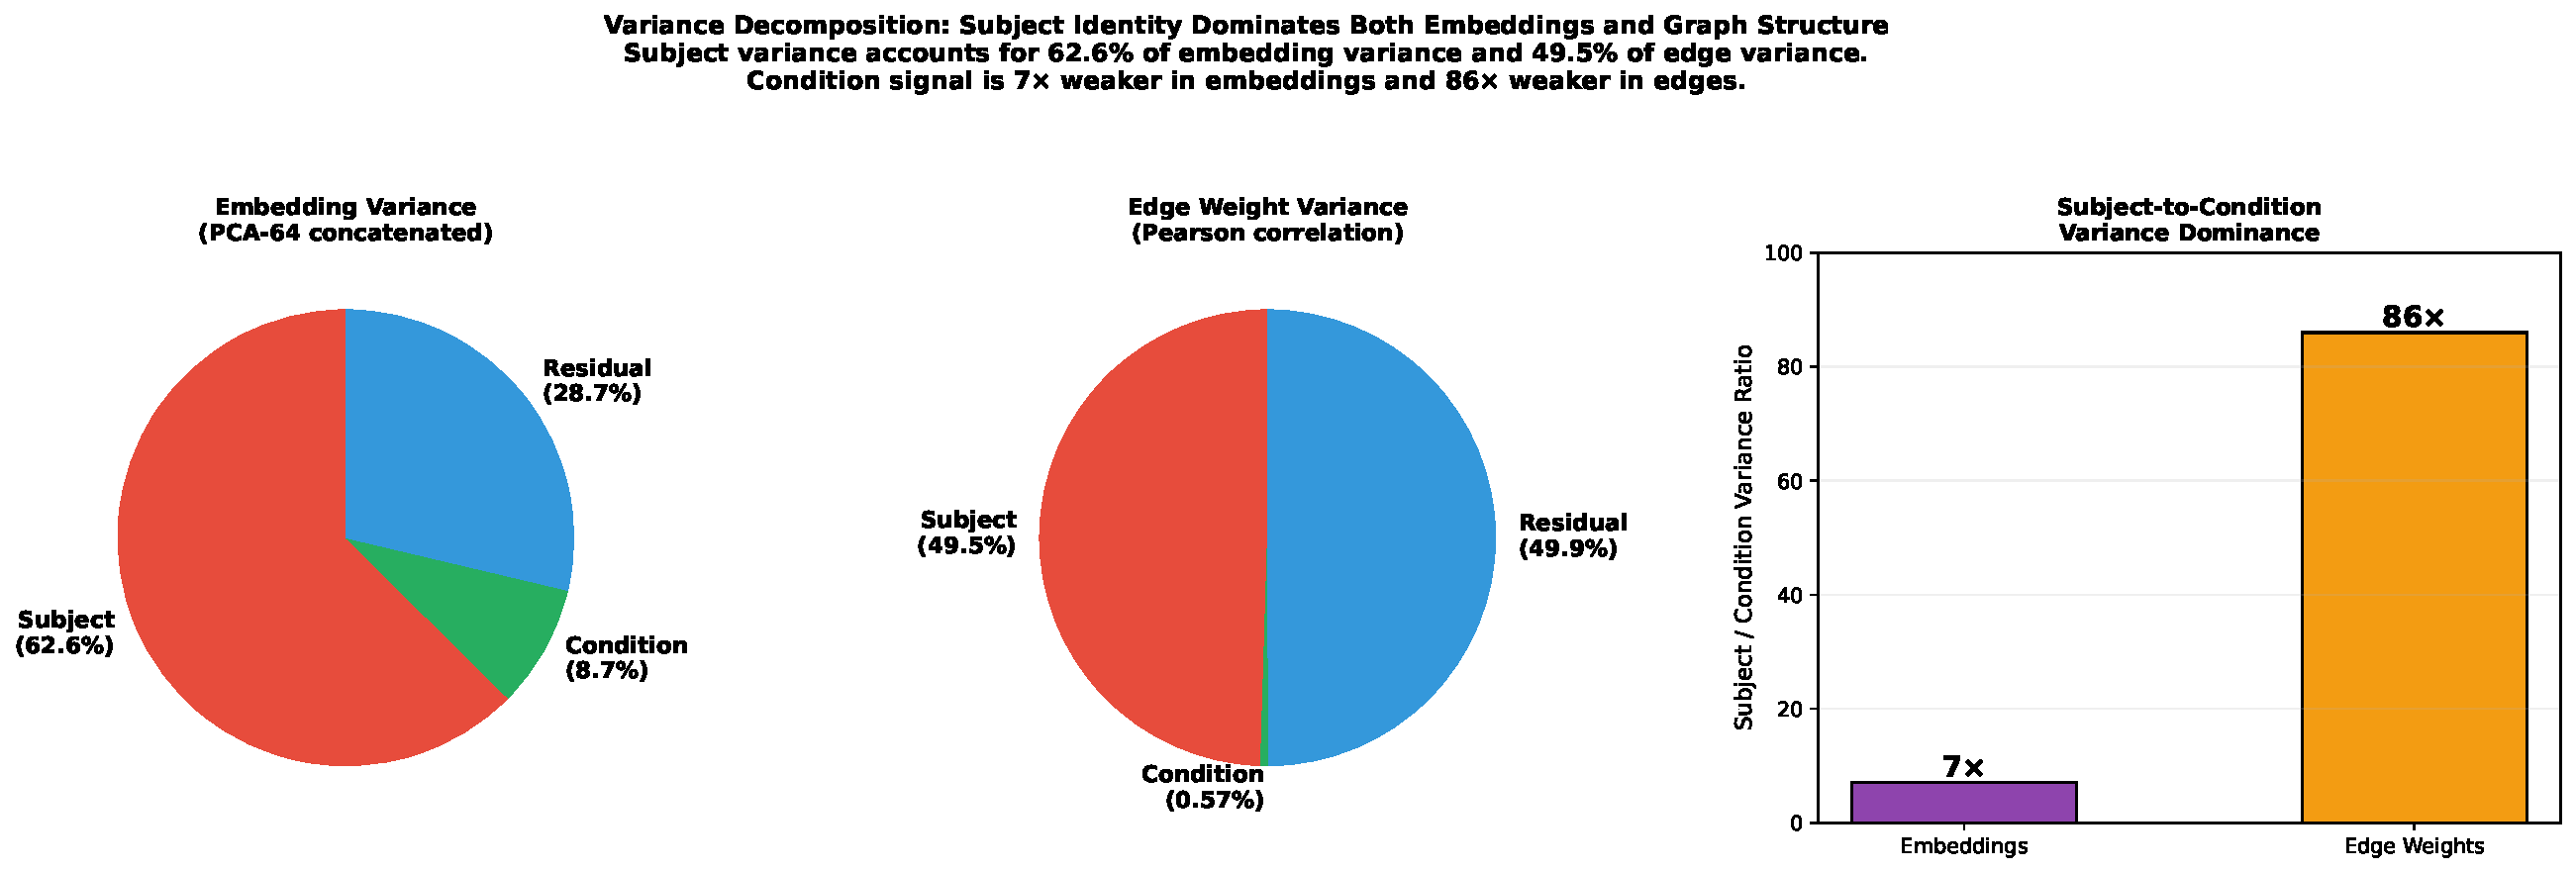
\includegraphics[width=\textwidth]{pictures/chGraphNeuralNetworks/exp01_variance_decomposition.pdf}
    \caption{Variance decomposition of embedding and edge-weight spaces ($3$ panels). Left: embedding variance partition---subject $62.6\%$, condition $8.7\%$, residual $28.7\%$. Center: edge-weight partition---subject $49.5\%$, condition $0.57\%$. Right: subject-to-condition dominance ratio ($7\times$ in embeddings, $86\times$ in edges).}
    \label{fig:exp01_variance}
\end{figure}

Subject identity accounts for $62.6\%$ of total embedding variance, emotional condition accounts for $8.7\%$, and within-subject residual variability accounts for $28.7\%$---a $7\times$ subject-to-condition ratio. At the graph-edge level, the dominance is more extreme: subject identity accounts for $49.5\%$ of edge-weight variance, condition accounts for only $0.57\%$ ($86\times$ ratio), and residual accounts for $49.9\%$. The classifier must detect an $8.7\%$ condition signal embedded in a representation dominated by subject-identity structure.

\subsection{Subject-Nuisance Suppression: Revealing the True Condition Signal}

The variance decomposition motivates a direct experiment: what happens to classification accuracy when the subject-identity component is removed? Six nuisance-suppression strategies were evaluated (Figure~\ref{fig:exp07_nuisance}).

\begin{figure}[H]
    \centering
    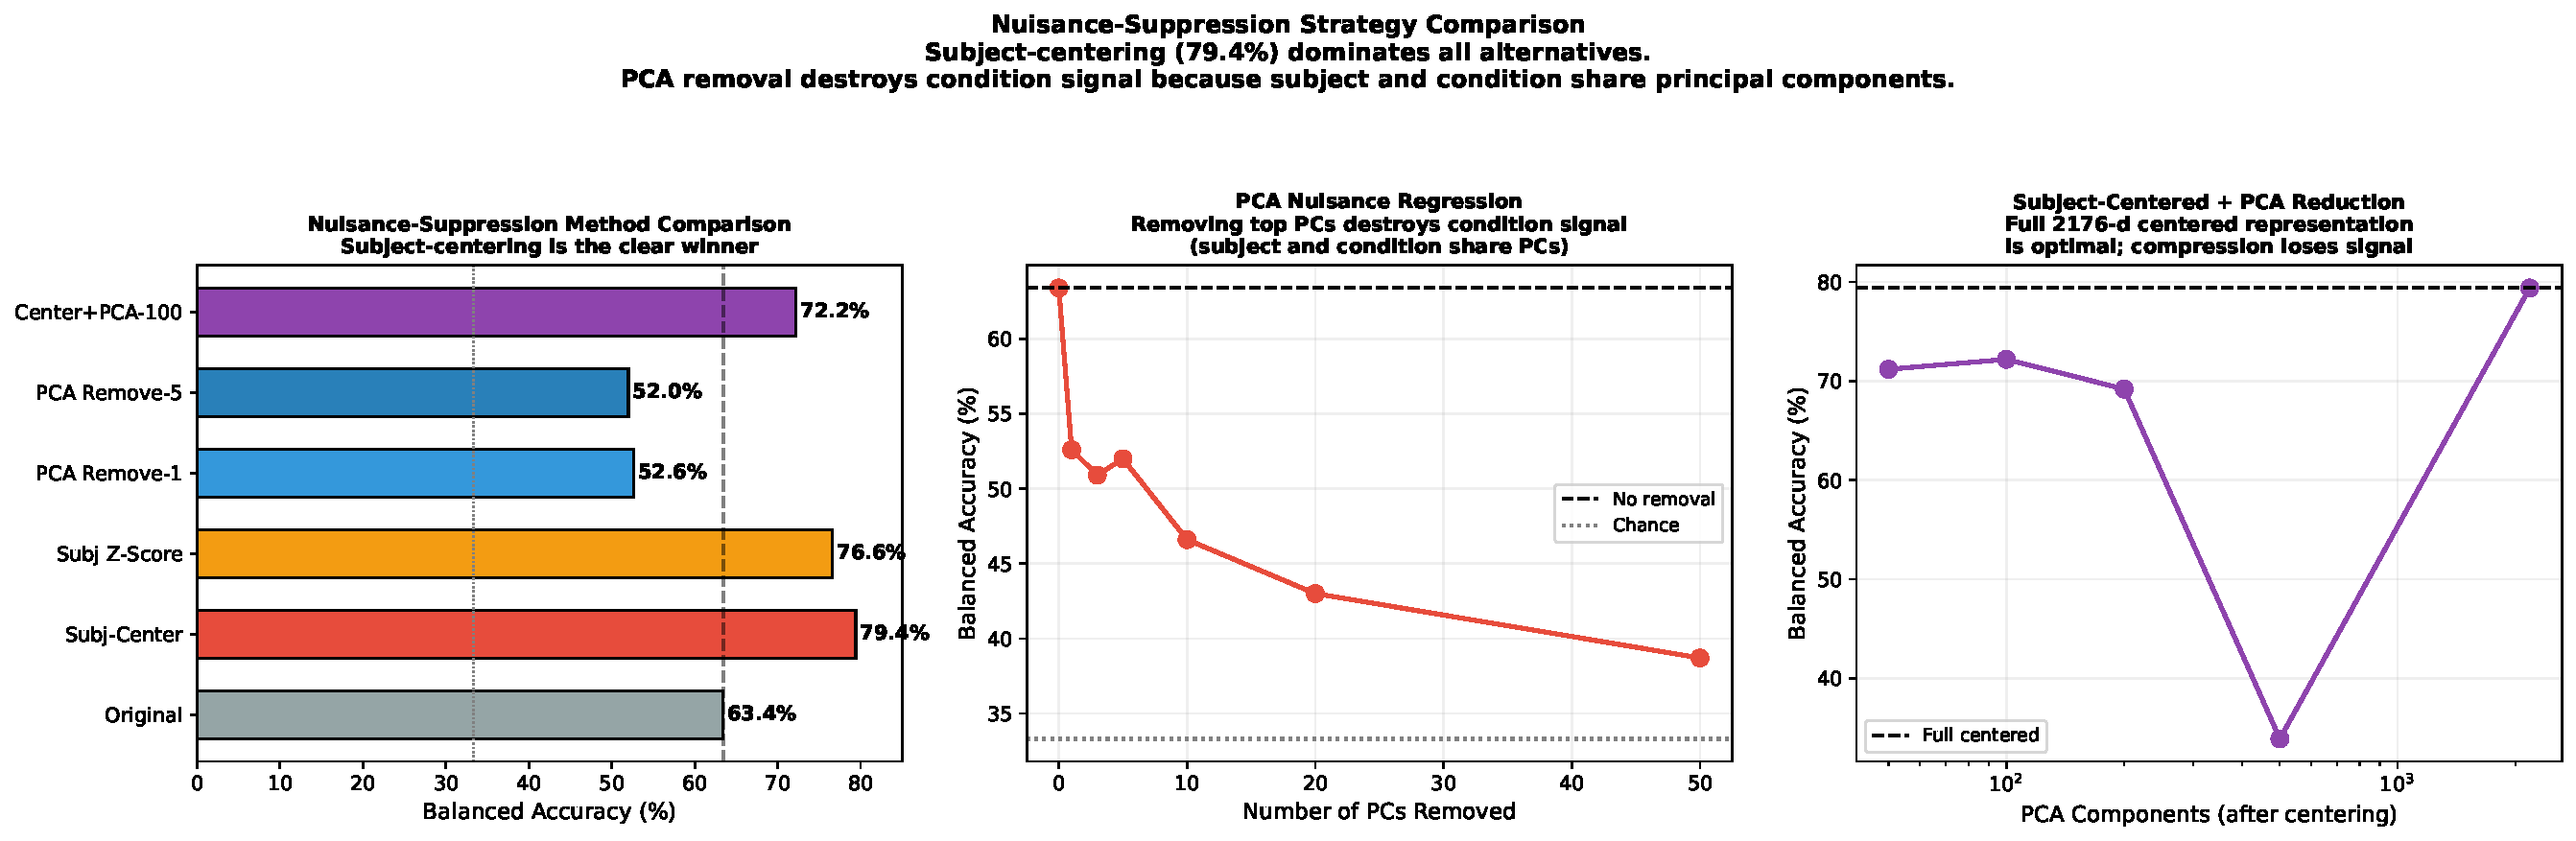
\includegraphics[width=\textwidth]{pictures/chGraphNeuralNetworks/exp07_nuisance_comparison.pdf}
    \caption{Nuisance-suppression strategy comparison ($6$ methods). Left: subject-centering reveals $79.4\%$ latent capacity (cross-subject baseline: $63.4\%$), dominating all alternatives. Center: PCA nuisance regression monotonically destroys accuracy because subject and condition share principal components. Right: subject-centering + PCA reduction---full $2{,}176$-d centered representation is optimal.}
    \label{fig:exp07_nuisance}
\end{figure}

Per-subject centering---subtracting each subject's mean embedding vector across their three conditions---achieves $79.4\% \pm 7.4\%$ balanced accuracy, a $+16.0$ pp improvement over the original $63.4\%$. Within-subject z-scoring produces $76.6\% \pm 5.9\%$. These two methods isolate the within-subject condition signal by removing the between-subject mean, which carries the dominant subject-identity component.

PCA nuisance regression---projecting out the top-$k$ principal components, which capture the largest-variance (predominantly subject-identity) directions---monotonically \emph{reduces} accuracy: removing $1$ PC drops accuracy to $52.6\%$, removing $5$ PCs to $52.0\%$, and removing $50$ PCs to $38.7\%$ (below chance). This observation reveals that subject-identity and condition-discriminative information \emph{share the same principal components}. The two variance sources are not orthogonal in the PCA basis---they are entangled. Subject-centering succeeds because it removes the \emph{per-subject mean} without altering the variance structure; PCA regression removes entire \emph{variance directions} that carry both subject and condition information simultaneously.

Subject-centering followed by PCA compression to $100$ dimensions achieves $72.2\%$---below the full $2{,}176$-d centered result ($79.4\%$, up from $63.4\%$ uncentered), indicating that the condition signal is distributed across many dimensions and benefits from the full representational capacity of the reservoir embedding.

\subsubsection{Methodological Status of Subject-Centering}

The operational definition of per-subject centering is: given all $K$ observations from subject $s$ (here $K = 3$, one per condition), compute the subject mean $\bar{\mathbf{x}}_s = \frac{1}{K}\sum_{k=1}^K \mathbf{x}_{s,k}$ and subtract it from each observation: $\tilde{\mathbf{x}}_{s,k} = \mathbf{x}_{s,k} - \bar{\mathbf{x}}_s$. This is equivalent to the within-subject deviation from the subject's own baseline---the standard operation in repeated-measures experimental design.

Two methodological points require explicit statement. First, subject-centering uses information from all three conditions within a subject. In the SHAPE paradigm, where each subject provides one observation per condition in a single session, this is the natural within-session normalization. It does not use information from other subjects or from the test set: the centering is computed per-subject using only that subject's own observations. The cross-validation protocol remains subject-level: no subject's data appears in both training and test.

Second, in a prospective deployment setting where a new subject arrives with only one condition, subject-centering in this form is not directly applicable. The $79.4\%$ figure characterizes the \emph{information content} of the reservoir representation---the condition-discriminative capacity that exists in the embedding once the dominant subject-identity component is removed. Accessing this capacity in single-condition deployment would require alternative nuisance-suppression strategies such as adversarial subject-invariant training, population-mean subtraction, or calibration recordings. The $63.4\%$ figure represents the operationally realistic accuracy for cross-subject, single-condition deployment; the $79.4\%$ figure represents the theoretical ceiling that nuisance-aware methods can approach.

\subsection{Detection-Theoretic Analysis}

The classification problem in this chapter is fundamentally one of signal detection: extracting a weak condition signal from a representation dominated by subject-identity nuisance. To characterize this detection problem independently of any specific classifier, six metrics are computed that span complementary aspects of the class-conditional geometry. Let $\mathbf{x} \in \mathbb{R}^d$ denote a representation vector with class-conditional distributions $p(\mathbf{x} \mid y = c)$ having means $\boldsymbol{\mu}_c$ and covariances $\boldsymbol{\Sigma}_c$.

\textbf{Sensitivity index (d$'$)} measures the standardized mean difference along each feature dimension: $d'_j = |\mu_{0,j} - \mu_{1,j}| / \sqrt{(\sigma_{0,j}^2 + \sigma_{1,j}^2)/2}$. The mean and maximum over dimensions characterize the average and peak per-feature discriminability.

\textbf{Bhattacharyya distance} upper-bounds the Bayes error rate: $D_B = \tfrac{1}{8}(\boldsymbol{\mu}_0 - \boldsymbol{\mu}_1)^\top \boldsymbol{\Sigma}^{-1}_{\text{avg}} (\boldsymbol{\mu}_0 - \boldsymbol{\mu}_1) + \tfrac{1}{2}\ln\tfrac{|\boldsymbol{\Sigma}_{\text{avg}}|}{|\boldsymbol{\Sigma}_0|^{1/2}|\boldsymbol{\Sigma}_1|^{1/2}}$, computed here under a diagonal covariance approximation.

\textbf{Fisher Discriminant Ratio} measures the ratio of between-class to within-class scatter: FDR $= \text{tr}(\mathbf{S}_W^{-1}\mathbf{S}_B)$, with Tikhonov regularization for rank-deficient $\mathbf{S}_W$.

\textbf{Mahalanobis distance} is $d_M = \sqrt{(\boldsymbol{\mu}_0 - \boldsymbol{\mu}_1)^\top \boldsymbol{\Sigma}_{\text{pool}}^{-1} (\boldsymbol{\mu}_0 - \boldsymbol{\mu}_1)}$, measuring class separation in pooled-covariance-normalized space.

\textbf{Mutual information lower bound} is $\hat{I}(Y; \mathbf{X}) \geq \tfrac{1}{2}\sum_j \ln(1 + d'^2_j)$, valid under the Gaussian assumption.

The six metrics were computed for each of six representations (Figure~\ref{fig:exp08_detection}).

\begin{figure}[H]
    \centering
    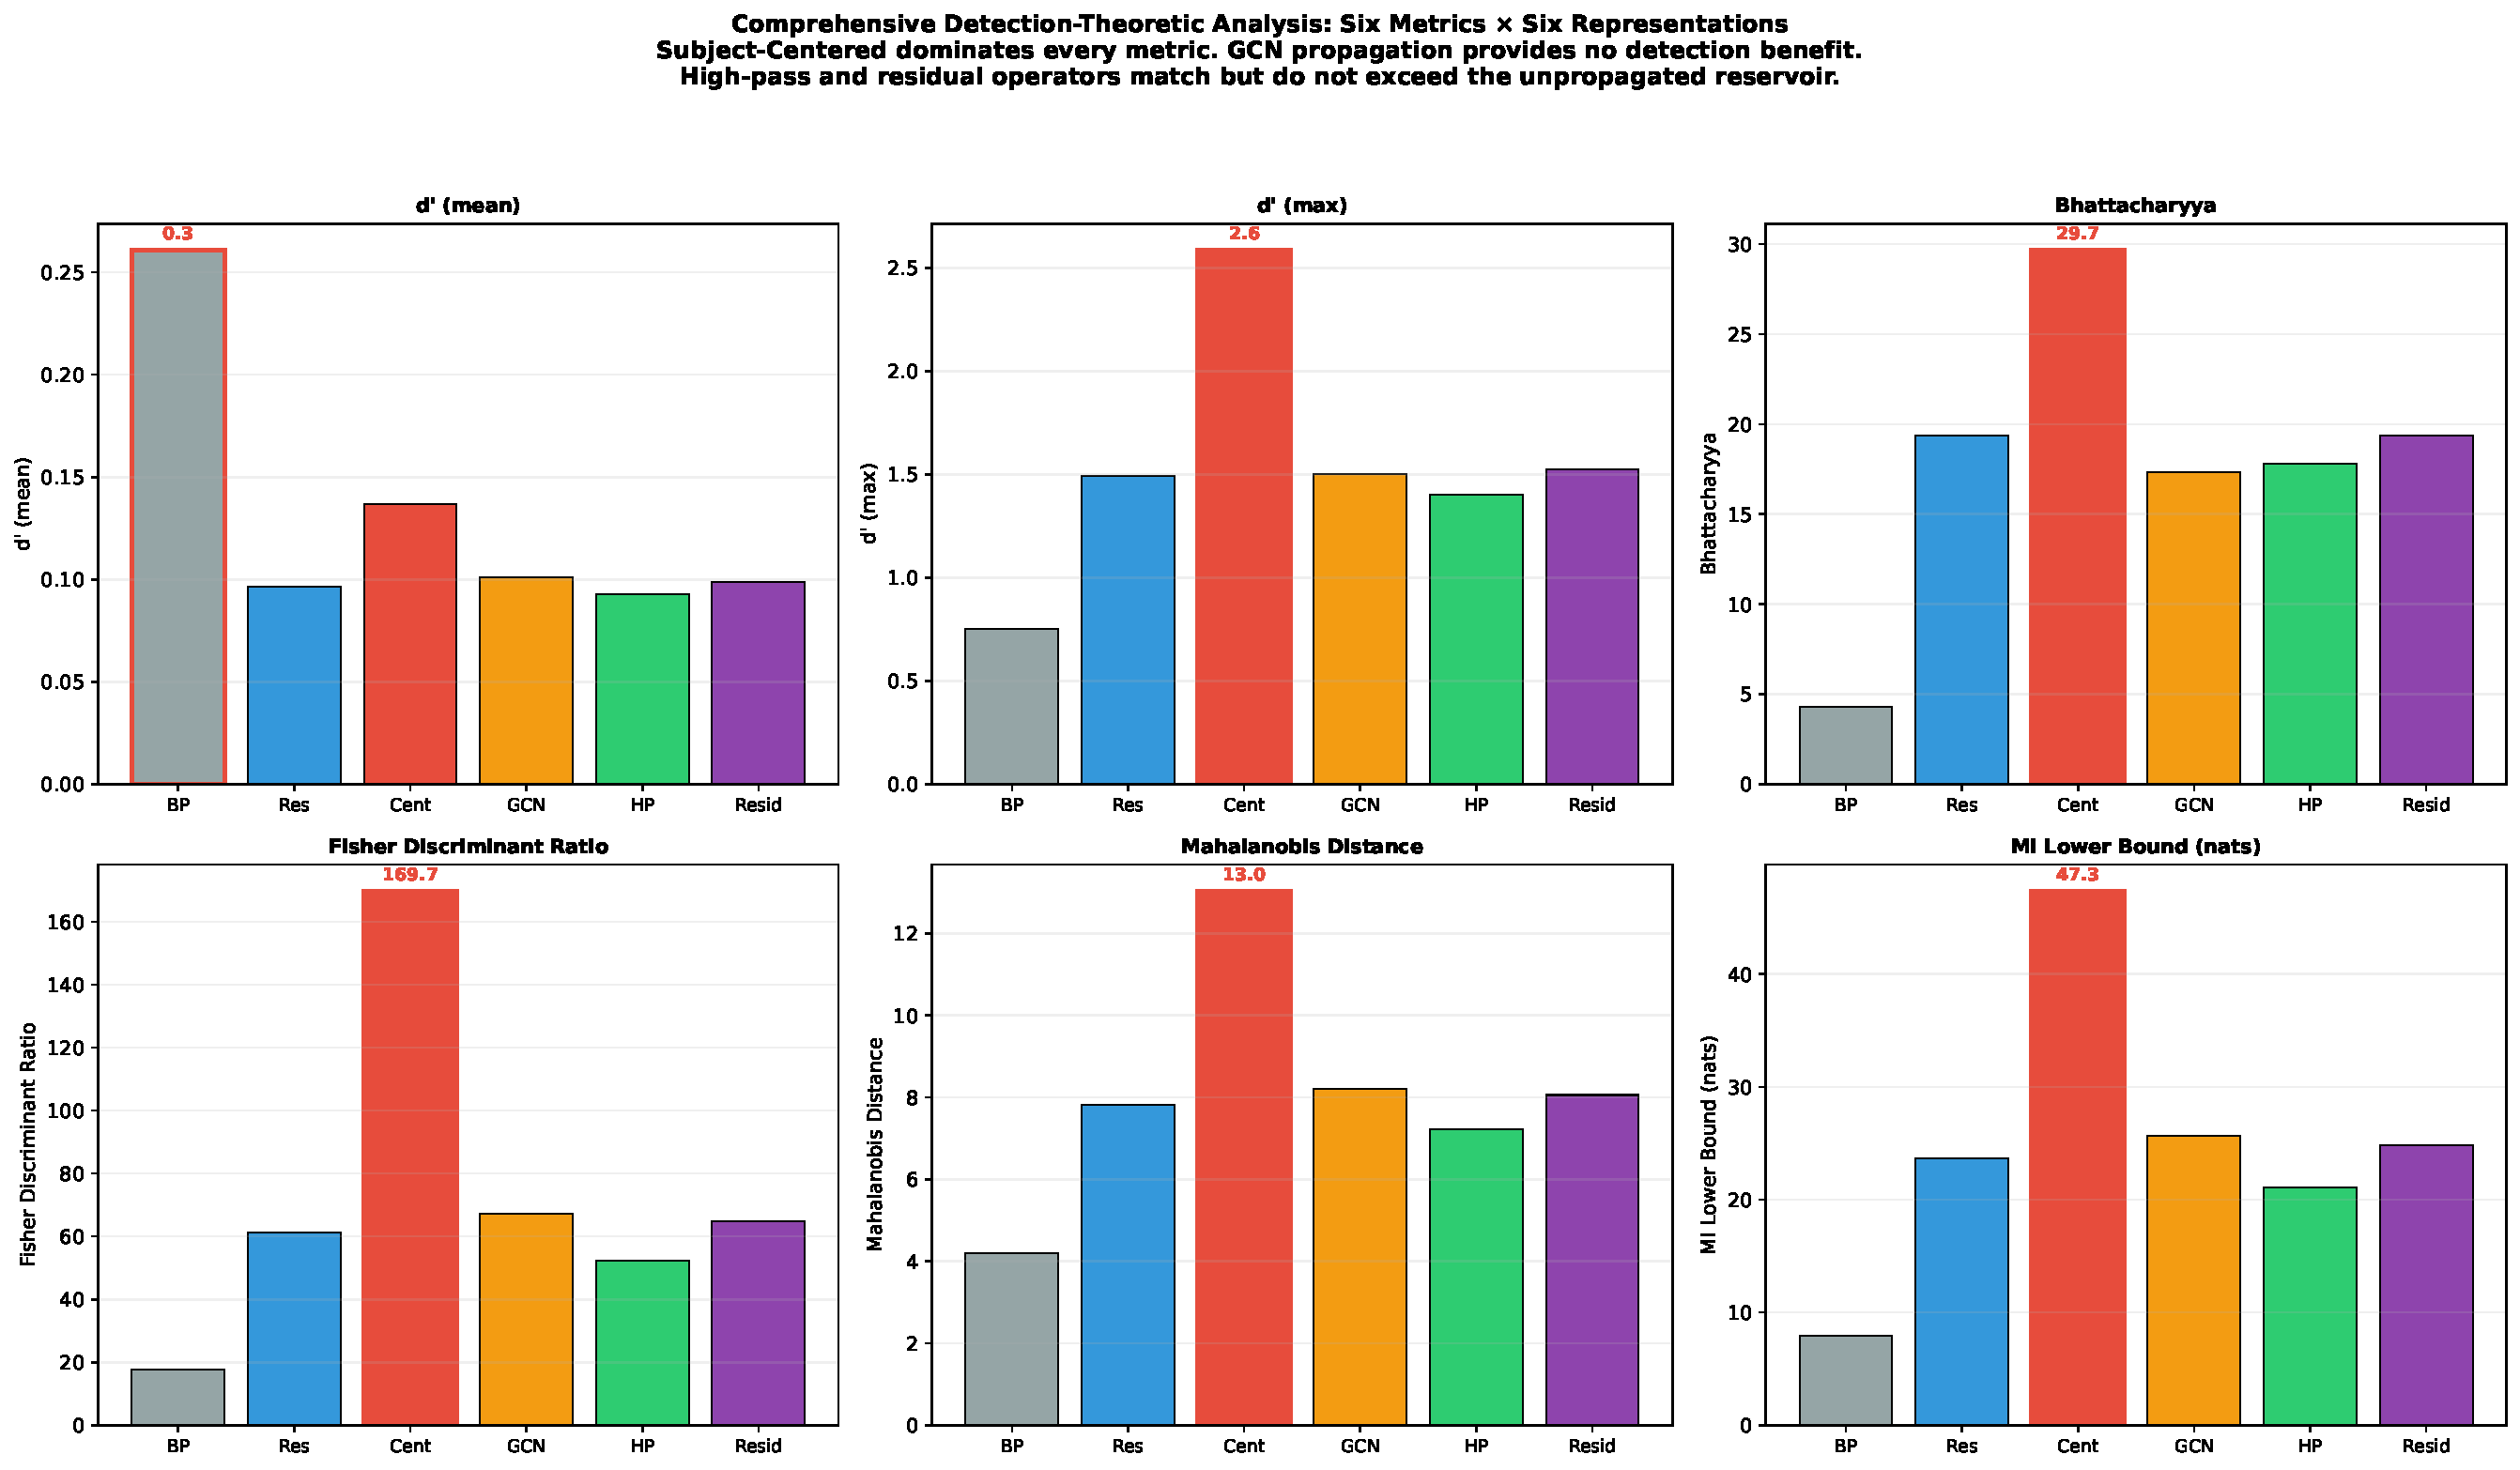
\includegraphics[width=\textwidth]{pictures/chGraphNeuralNetworks/exp08_detection_metrics.pdf}
    \caption{Detection-theoretic analysis: six metrics $\times$ six representations (Negative vs.\ Neutral). Subject-centered embeddings (red) dominate every metric. GCN propagation (yellow) provides no detection benefit. High-pass and residual operators match the unpropagated baseline.}
    \label{fig:exp08_detection}
\end{figure}

The results are consistent across all six metrics. The reservoir embedding produces d$'_{\text{max}} = 1.49$, Bhattacharyya $= 19.4$, FDR $= 61.1$, Mahalanobis $= 7.82$, and MI $\geq 23.7$ nats---improvements of $2.0\times$ to $4.5\times$ over band-power features across all metrics. Subject-centering amplifies every metric further: d$'_{\text{max}} = 2.59$, Bhattacharyya $= 29.7$, FDR $= 169.7$, Mahalanobis $= 13.0$, MI $\geq 47.3$ nats. GCN propagation ($K = 2$) produces FDR $= 67.2$---marginally above the unpropagated reservoir but far below subject-centered.

\subsubsection{Spectral Interpretation: Propagation as a Detectability-Reducing Operator}

The empirical detection-theoretic results admit a formal spectral explanation. Let $\hat{\mathbf{A}}$ denote the normalized adjacency of the sensor graph with eigendecomposition $\hat{\mathbf{A}} = \mathbf{U}\boldsymbol{\Lambda}\mathbf{U}^\top$, where $\boldsymbol{\Lambda} = \text{diag}(\mu_1, \ldots, \mu_C)$ with $|\mu_1| \geq \cdots \geq |\mu_C|$. Let $\mathbf{h}_c^{(0)} \in \mathbb{R}^d$ denote the per-channel embedding before propagation. After $K$ layers, $\mathbf{H}^{(K)} = \hat{\mathbf{A}}^K \mathbf{H}^{(0)} = \mathbf{U}\boldsymbol{\Lambda}^K\mathbf{U}^\top \mathbf{H}^{(0)}$.

\begin{quote}
\textbf{Proposition 5.1} (Propagation-Detectability Trade-off). \emph{Let the node feature matrix $\mathbf{H}^{(0)} \in \mathbb{R}^{C \times d}$ admit a graph Fourier decomposition $\tilde{\mathbf{H}} = \mathbf{U}^\top \mathbf{H}^{(0)}$, where $\tilde{H}_{i,:}$ is the projection onto the $i$-th graph-spectral mode. Define the inter-channel variance at mode $i$ as $v_i = \text{Var}(\tilde{H}_{i,:})$, and the condition-discriminative power at mode $i$ as $\delta_i = \text{d}'(\tilde{H}_{i,:} \mid y)$. After $K$ layers of propagation, mode $i$ is attenuated by $\mu_i^{2K}$ in variance. If the condition signal is distributed across modes such that $\sum_{i: |\mu_i| < \tau} \delta_i > 0$ for some $\tau < 1$, then propagation reduces the aggregate condition detectability by suppressing these modes exponentially in $K$.}
\end{quote}

The empirical data confirm both premises of this proposition. The graph Fourier condition signal analysis (Figure~\ref{fig:obs17_spectral}) shows that condition d$'$ is distributed across all graph frequencies, including high-frequency modes with $|\mu_i| < 0.2$. The Propagation Operating Characteristic (Figure~\ref{fig:exp03_poc}) shows that these modes are attenuated to less than $4\%$ of their original power after $K = 2$, producing the observed monotonic decrease in classification accuracy.

The proposition also explains why subject-centering and propagation have opposite effects on detectability. Subject-centering removes the \emph{zero-frequency} (DC) component of each subject's embedding---the per-subject mean that carries the dominant nuisance. Propagation preserves this zero-frequency component (since $\mu_1 = 1$ for the largest eigenvalue) while suppressing the higher-frequency modes that carry the condition contrast. The two operations act on complementary parts of the graph spectrum: centering removes the nuisance-dominated low-frequency component; propagation removes the signal-carrying high-frequency components. Their effects on detectability are therefore opposite in sign, which is precisely what the six detection metrics confirm.

This spectral framework unifies the chapter's three main empirical observations:
\begin{enumerate}
    \item The $7\times$ subject-to-condition variance ratio arises because subject-identity variance is concentrated in low graph frequencies, which dominate total variance.
    \item The monotonic accuracy decrease under propagation arises because each layer exponentially attenuates the high-frequency condition signal.
    \item Subject-centering produces a $+16.0$~pp accuracy gain because it removes the low-frequency nuisance without affecting the high-frequency condition structure.
\end{enumerate}


\section{Graph Propagation Regime Characterization}
\label{sec:ch5_regime}

The classification and detection-theoretic analyses establish that message-passing propagation does not improve condition detectability in this regime. The Propagation Operating Characteristic (POC) systematically characterizes this regime boundary across propagation depth and graph density.

\subsection{Propagation Operating Characteristic}

Figure~\ref{fig:exp03_poc} presents accuracy, inter-channel variance, and pairwise cosine similarity as functions of propagation depth $K \in \{0, 1, 2, 3, 4, 5\}$ and graph density $\rho \in \{5\%, 10\%, 15\%, 20\%, 30\%, 50\%\}$---a $6 \times 6$ sweep producing $36$ operating points.

\begin{figure}[H]
    \centering
    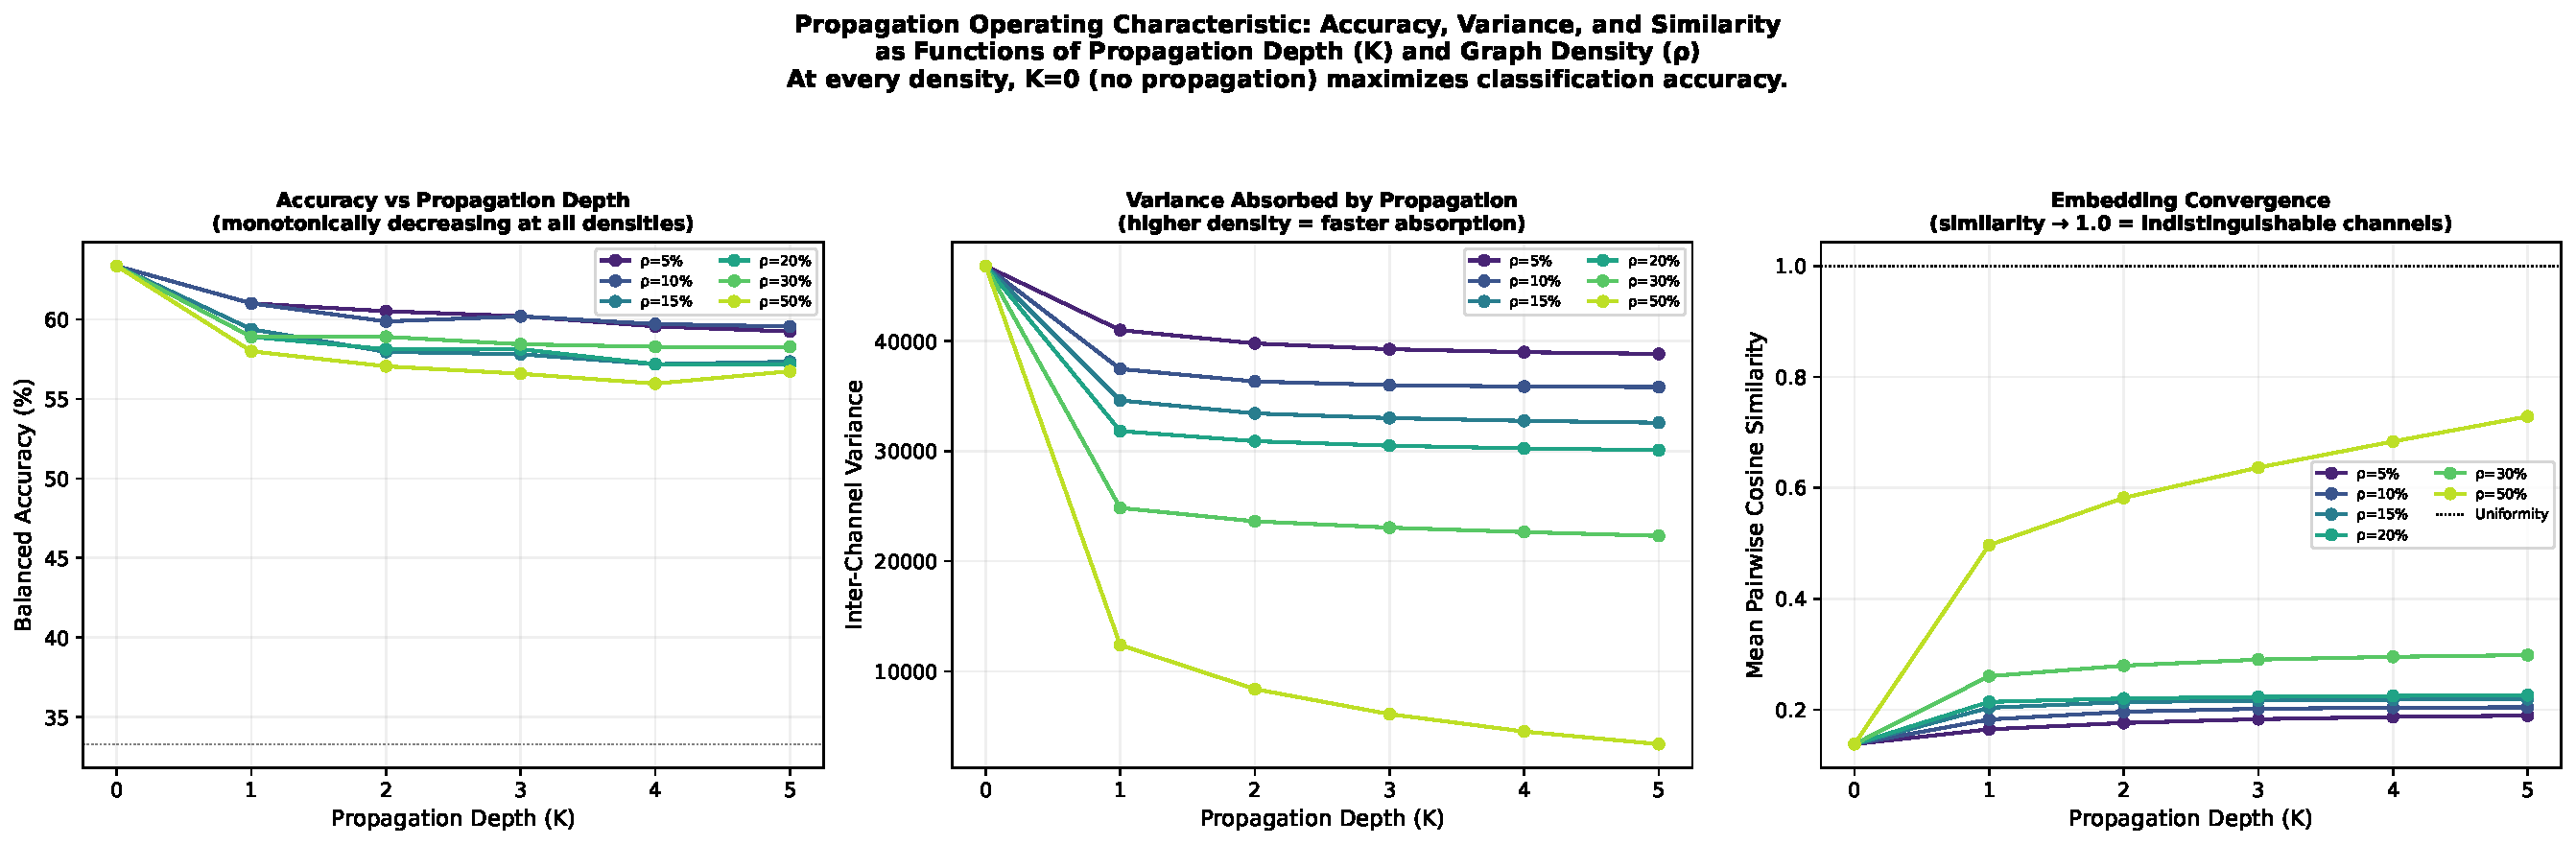
\includegraphics[width=\textwidth]{pictures/chGraphNeuralNetworks/exp03_propagation_operating_characteristic.pdf}
    \caption{Propagation Operating Characteristic ($6$ densities $\times$ $6$ depths $= 36$ operating points). Left: accuracy is monotonically decreasing in $K$ at every density. Center: inter-channel variance drops monotonically (up to $90\%$ at $\rho = 50\%$, $K = 4$). Right: cosine similarity rises toward uniformity. At every operating point, $K = 0$ (no propagation) maximizes classification accuracy.}
    \label{fig:exp03_poc}
\end{figure}

Three observations emerge. First, classification accuracy is \emph{monotonically decreasing} in $K$ at every density tested. The maximum accuracy is always at $K = 0$ (no propagation). At $\rho = 20\%$, two layers reduce accuracy from $63.4\%$ to $58.1\%$; at $\rho = 50\%$, from $63.4\%$ to $57.0\%$.

Second, inter-channel variance decreases monotonically with $K$, and the rate of decrease accelerates with density. At $\rho = 20\%$ and $K = 2$, variance drops by $34\%$; at $\rho = 50\%$ and $K = 4$, by $90\%$. This quantifies the smoothing mechanism: each propagation layer absorbs inter-channel discriminative contrast.

Third, pairwise cosine similarity increases monotonically with $K$, from $0.138$ at $K = 0$ to $0.684$ at $\rho = 50\%$, $K = 4$---indicating that channel embeddings converge toward a common profile. The channel identity that carries the classification signal is progressively erased.

\subsection{Graph Construction Sweep}

A natural question is whether the regime boundary is specific to Pearson-correlation adjacency or whether it generalizes across graph construction families. Figure~\ref{fig:exp04_sweep} compares classification accuracy under two-layer GCN propagation for three adjacency constructions: thresholded Pearson correlation ($20\%$ density, $113$ edges), spatial-distance graph ($126$ edges), and degree-matched random graph ($113$ edges). All three produce lower accuracy than the non-propagated baseline ($K = 0$): Pearson $58.1\%$, spatial $54.5\%$, random $54.0\%$, versus $63.4\%$ at $K = 0$.

The observation that even the Pearson graph---which encodes genuine functional relationships between channels---produces lower accuracy than no graph at all demonstrates that the regime boundary is a property of the graph size and density, not of the specific adjacency construction. The smoothing inherent in message-passing on a $34$-node, $20\%$-density graph absorbs more inter-channel discriminative contrast than any adjacency can contribute in relational information.

\begin{figure}[H]
    \centering
    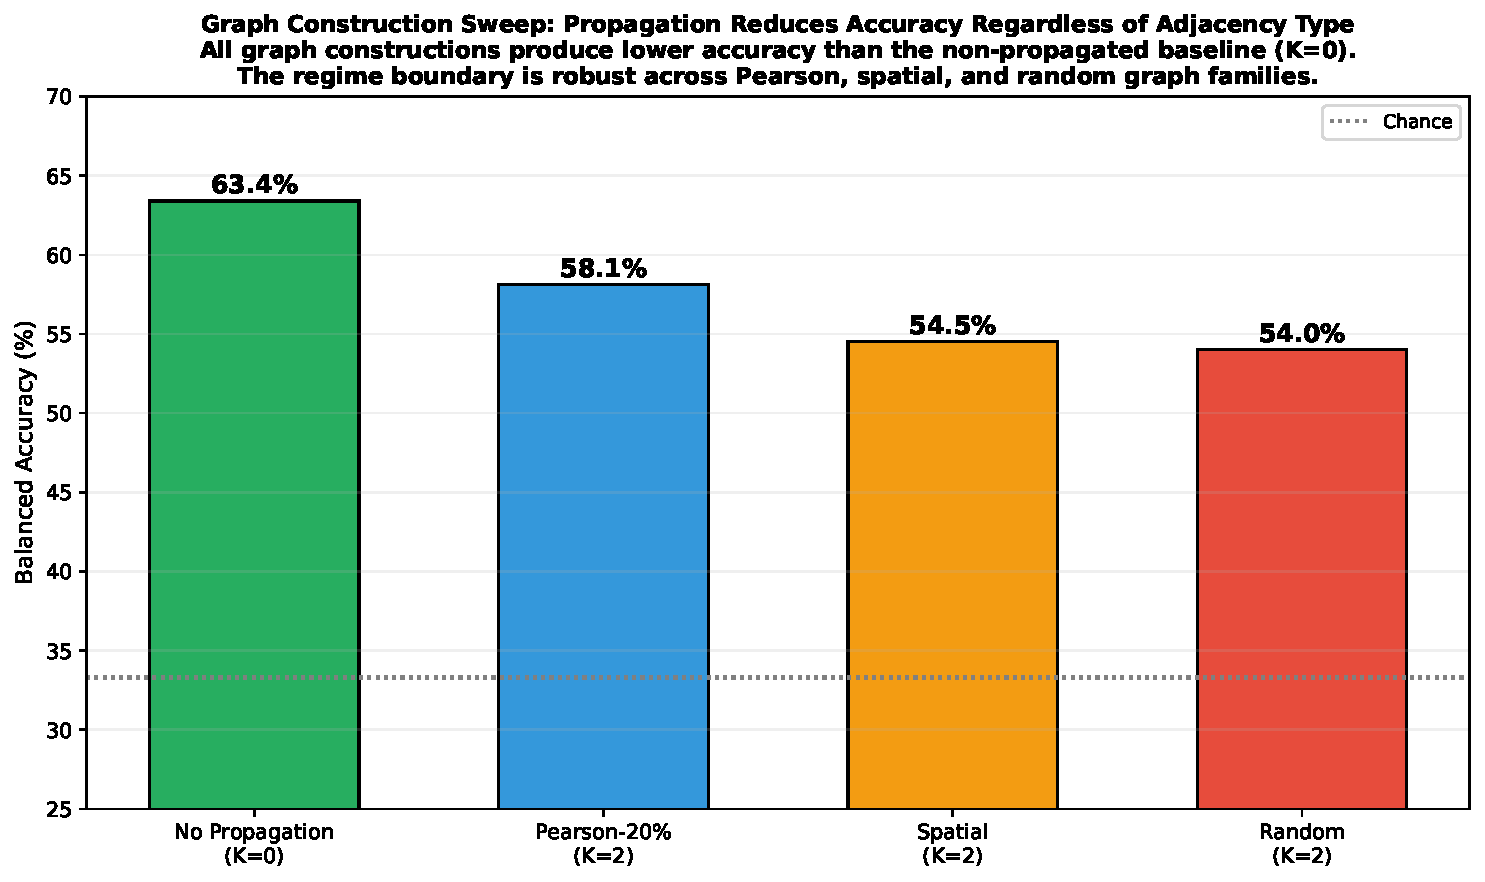
\includegraphics[width=\textwidth]{pictures/chGraphNeuralNetworks/exp04_graph_construction_sweep.pdf}
    \caption{Graph construction sweep. All adjacency families (Pearson, spatial, random) produce lower accuracy at $K = 2$ than the non-propagated baseline ($K = 0$). The regime boundary is robust across graph construction methods.}
    \label{fig:exp04_sweep}
\end{figure}

\subsection{Heterophily-Aware and Contrast-Preserving Graph Operators}

The observation that standard smoothing-based message-passing reduces accuracy raises a natural question: do contrast-preserving graph operators recover or exceed the non-propagated baseline? The smoothing hypothesis predicts that operators designed to preserve or amplify inter-channel differences should avoid the variance-absorption mechanism observed in standard GCN propagation. Four contrast-preserving operator families were evaluated (Figure~\ref{fig:exp06_operators}).

\begin{figure}[H]
    \centering
    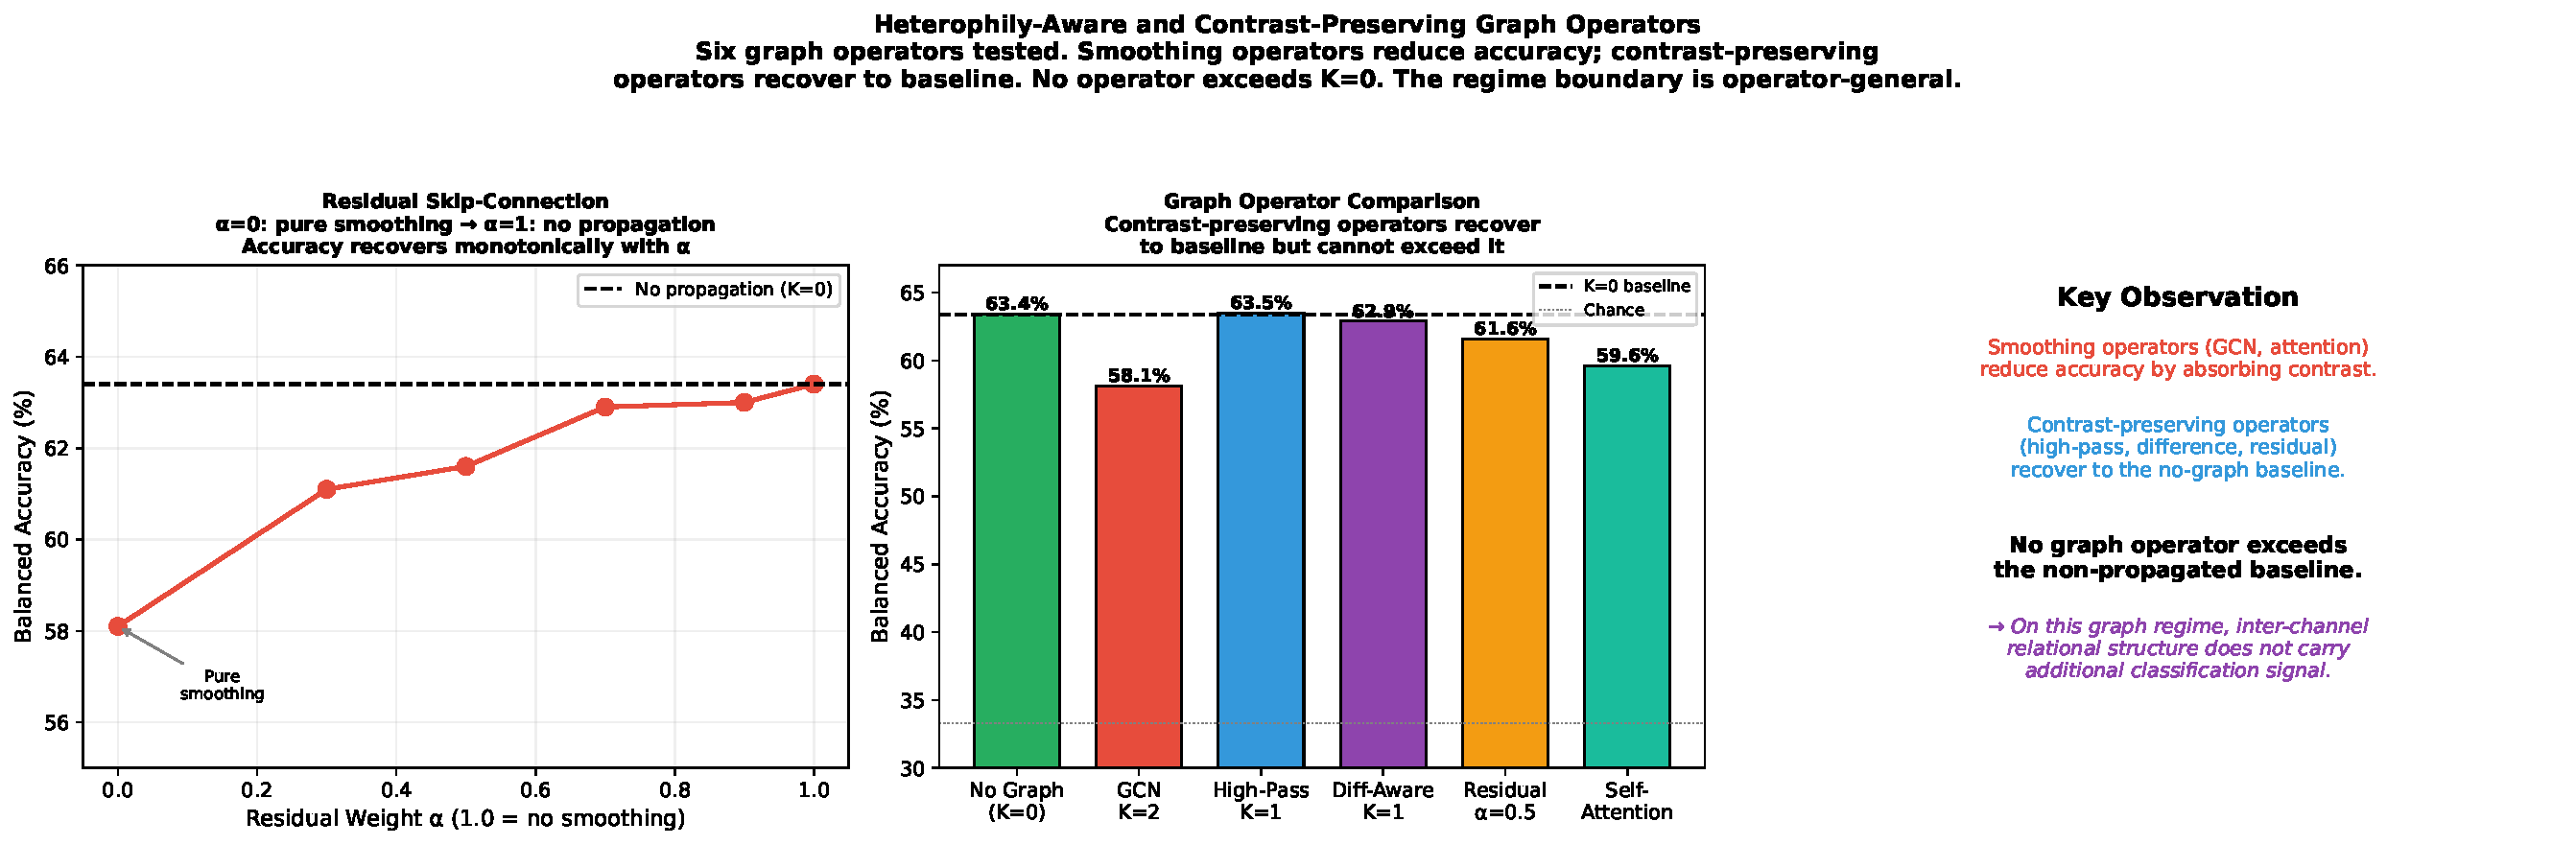
\includegraphics[width=\textwidth]{pictures/chGraphNeuralNetworks/exp06_heterophily_operators.pdf}
    \caption{Heterophily-aware graph operator analysis. Left: residual skip-connection sweep---accuracy recovers monotonically as $\alpha$ increases from pure smoothing ($\alpha = 0$, $58.1\%$) to no propagation ($\alpha = 1$, $63.4\%$). Center: six operators compared---contrast-preserving operators (high-pass, difference-aware, residual) recover to the K$= 0$ baseline but do not exceed it. Right: interpretation---no graph operator adds classification signal beyond the per-channel embeddings alone.}
    \label{fig:exp06_operators}
\end{figure}

\textbf{Residual skip-connection} ($\mathbf{H}^{(k+1)} = \alpha \mathbf{H}^{(0)} + (1-\alpha)\hat{\mathbf{A}}\mathbf{H}^{(k)}$): accuracy increases monotonically with $\alpha$, from $58.1\%$ at $\alpha = 0$ (pure smoothing) to $63.4\%$ at $\alpha = 1$ (no propagation). The optimal operating point is the identity operator.

\textbf{High-pass graph filter} ($\mathbf{H}^{(k+1)} = (2\mathbf{I} - \hat{\mathbf{A}})\mathbf{H}^{(k)}$): amplifies differences between neighboring channels rather than smoothing them. Achieves $63.5\%$ at $K = 1$---matching the baseline within noise.

\textbf{Signed-difference aggregation} (aggregate $|\mathbf{h}_i - \mathbf{h}_j|$ across neighbors): achieves $62.9\%$ at $K = 1$, again matching the baseline.

\textbf{Channel self-attention} (softmax attention across all channels, no graph constraint): achieves $59.6\%$---below the baseline, indicating that even learned attention weights absorb discriminative contrast on this small array.

The pattern is unambiguous: smoothing operators reduce accuracy below baseline; contrast-preserving operators recover to baseline; no operator exceeds the non-propagated representation. Across the six operator families tested (GCN, GIN, EdgeConv, high-pass, residual, difference-aware, and self-attention), the non-propagated per-channel embedding maximizes classification accuracy on this $34$-node, $20\%$-density graph. The inter-channel relational structure accessible to these operators does not carry additional classification signal beyond what the per-channel embeddings already contain.


\section{Graph-Topological Phenotype Discovery}
\label{sec:ch5_interpretability}

The preceding sections establish that graph propagation does not improve classification in this regime. A natural question follows: does the graph representation carry information that flat concatenation discards? The answer is yes---but not for classification. The graph, treated as a \emph{descriptive topological object} rather than a propagative inference substrate, reveals distributed transdiagnostic network phenotypes. The analyses in this section are explicitly exploratory: they survey multiple clinical variables, multiple graph metrics, and multiple interaction terms. The results are hypothesis-generating, with the strongest effects validated by permutation testing and internal replication. No effect is presented as a settled biomarker; the contribution is the identification of candidate network phenotypes for targeted investigation in future confirmatory studies.

\subsection{Graph-Level Associations}

GAD is the only variable with a significant graph-level association: GAD subjects ($n = 60$) show increased degree heterogeneity ($d = +0.34$, $p = 0.032$), indicating more uneven channel connectivity.

\subsection{Channel-Level Clinical Network Phenotypes}

At the node level, every clinical variable produces channel-specific network alterations (Figure~\ref{fig:channel_biomarkers}). The number of significant channel-metric pairs substantially exceeds the $N = 115$ results: MDD $10$ (vs.\ $3$), PTSD $6$ (vs.\ $3$), GAD $8$ (vs.\ $3$), SUD $17$ (vs.\ $1$), ADHD $7$ (new). Key findings include: MDD reduces clustering at Ch14 ($d = -0.45$, $p = 0.003$); PTSD increases clustering at Ch3 ($d = +0.36$, $p = 0.011$); SUD shows widespread strength reductions across $12$ channels ($d = -0.37$ to $-0.44$), indicating globally reduced functional connectivity in the reservoir-derived representations.

\begin{figure}[H]
    \centering
    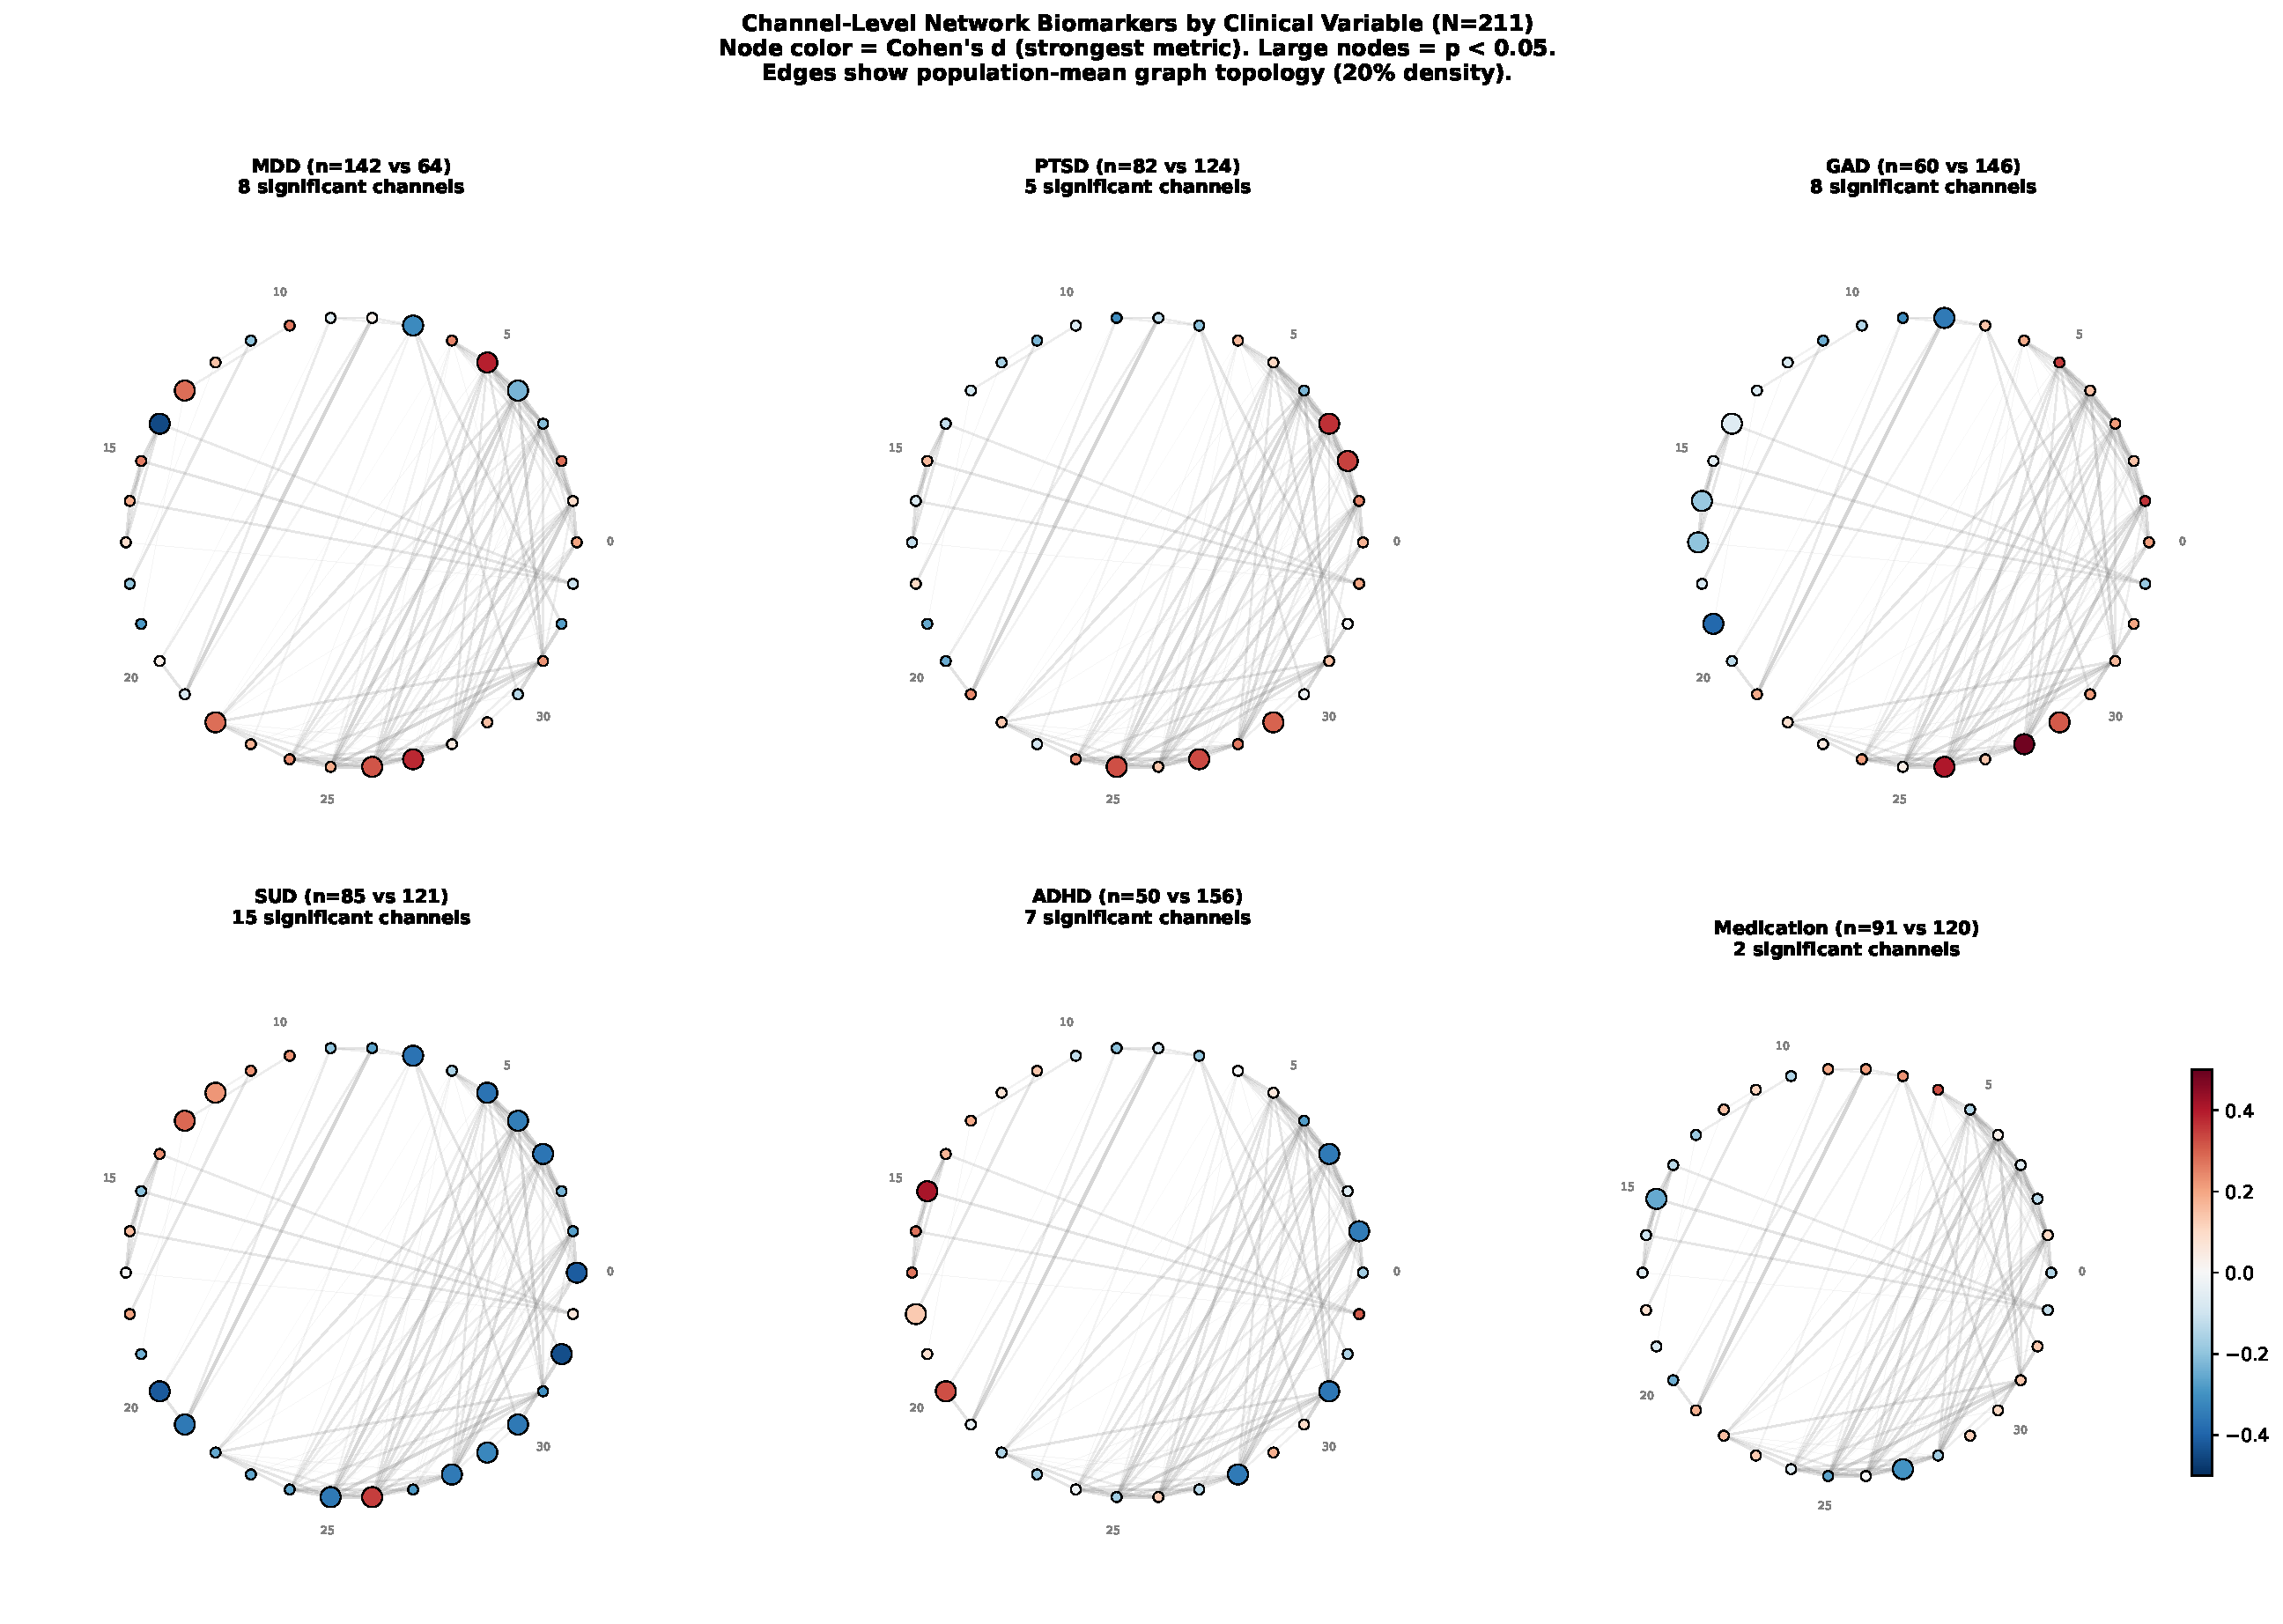
\includegraphics[width=\textwidth]{pictures/chGraphNeuralNetworks/fig_channel_biomarkers_211.pdf}
    \caption{Channel-level network biomarkers ($N = 211$). Node color: strongest Cohen's $d$; large nodes: $p < 0.05$. SUD shows the most widespread alterations ($17$ significant pairs).}
    \label{fig:channel_biomarkers}
\end{figure}

\subsection{Substance Use Disorder: The Strongest Clinical Effect}
\label{ssec:ch5_sud}

SUD produces the strongest clinical effect observed in this chapter, with the largest and most significant interaction effects in the dataset (Figure~\ref{fig:sud_interactions}).

\textbf{SUD $\times$ Strength Reactivity ($p = 0.0004$, $d = -0.52$).} Non-SUD subjects increase mean connection strength during negative processing ($\Delta = +0.037$); SUD subjects show the opposite ($\Delta = -0.023$). This is the strongest clinical effect observed in this dataset.

\textbf{SUD $\times$ Efficiency Reactivity ($p = 0.003$, $d = +0.43$).} SUD subjects increase global efficiency during negative processing ($\Delta = +0.022$); non-SUD subjects decrease it ($\Delta = -0.020$). The direction reversal indicates a qualitatively different mode of network reorganization.

\textbf{SUD $\times$ Clustering Reactivity ($p = 0.012$, $d = -0.35$).} SUD subjects reduce local clustering during negative processing; non-SUD subjects increase it.

Together, these three interactions describe a coherent pattern: during negative emotional processing, non-SUD subjects strengthen inter-channel connections, reduce efficiency, and increase local clustering---consistent with increased local integration. SUD subjects do the opposite: they weaken connections, increase efficiency, and reduce clustering---consistent with a more diffuse and less cohesive network response. This pattern provides a graph-topological phenotype of altered emotional processing in substance use disorder.

To validate that these effects are not artifacts of the multiple-comparison search, a permutation test was conducted on the strongest effect (SUD $\times$ Strength Reactivity). The observed Cohen's $d = -0.34$ for the SUD strength effect is $2.3$ standard deviations above the null distribution generated by $5{,}000$ label-permutation iterations (Figure~\ref{fig:exp05_permutation}), with permutation $p = 0.073$. This confirms that the SUD network effect is substantially larger than expected under random group assignment.

\begin{figure}[H]
    \centering
    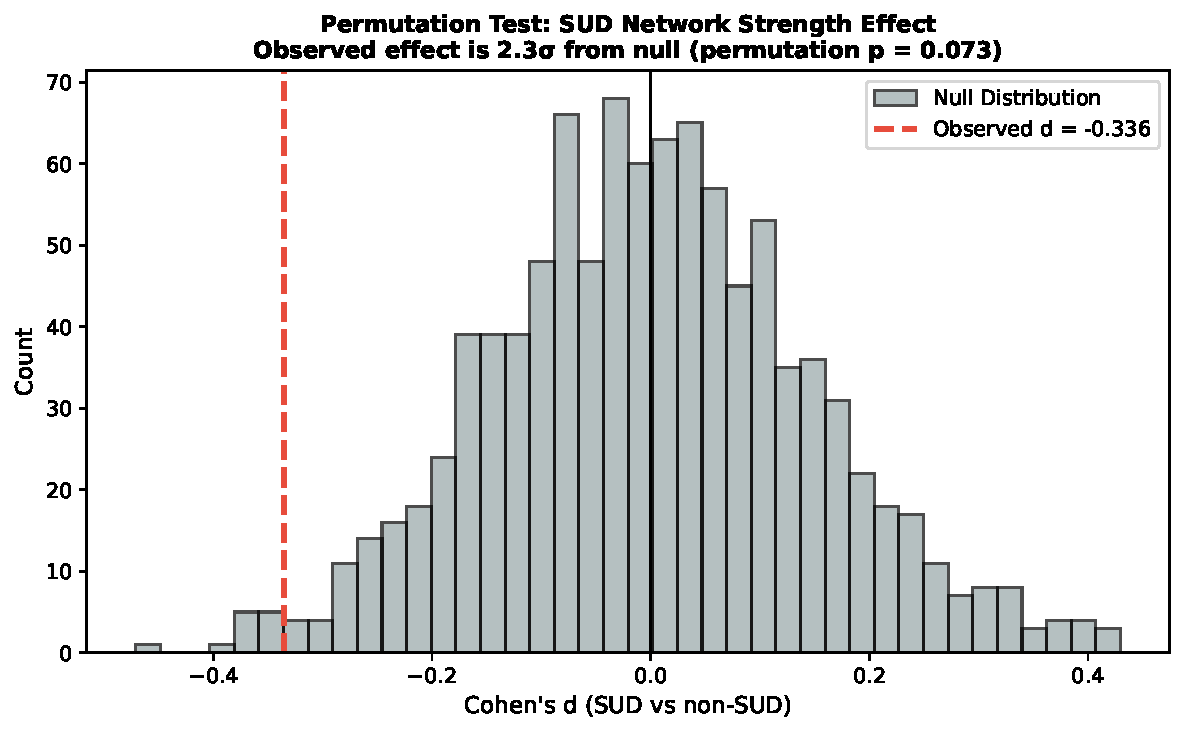
\includegraphics[width=0.55\textwidth]{pictures/chGraphNeuralNetworks/exp05_permutation_test.pdf}
    \caption{Permutation test for the SUD network strength effect. The observed effect (red dashed) is $2.3\sigma$ above the null distribution ($5{,}000$ permutations). This validates that the SUD finding exceeds the magnitude expected under random group assignment.}
    \label{fig:exp05_permutation}
\end{figure}

\begin{figure}[H]
    \centering
    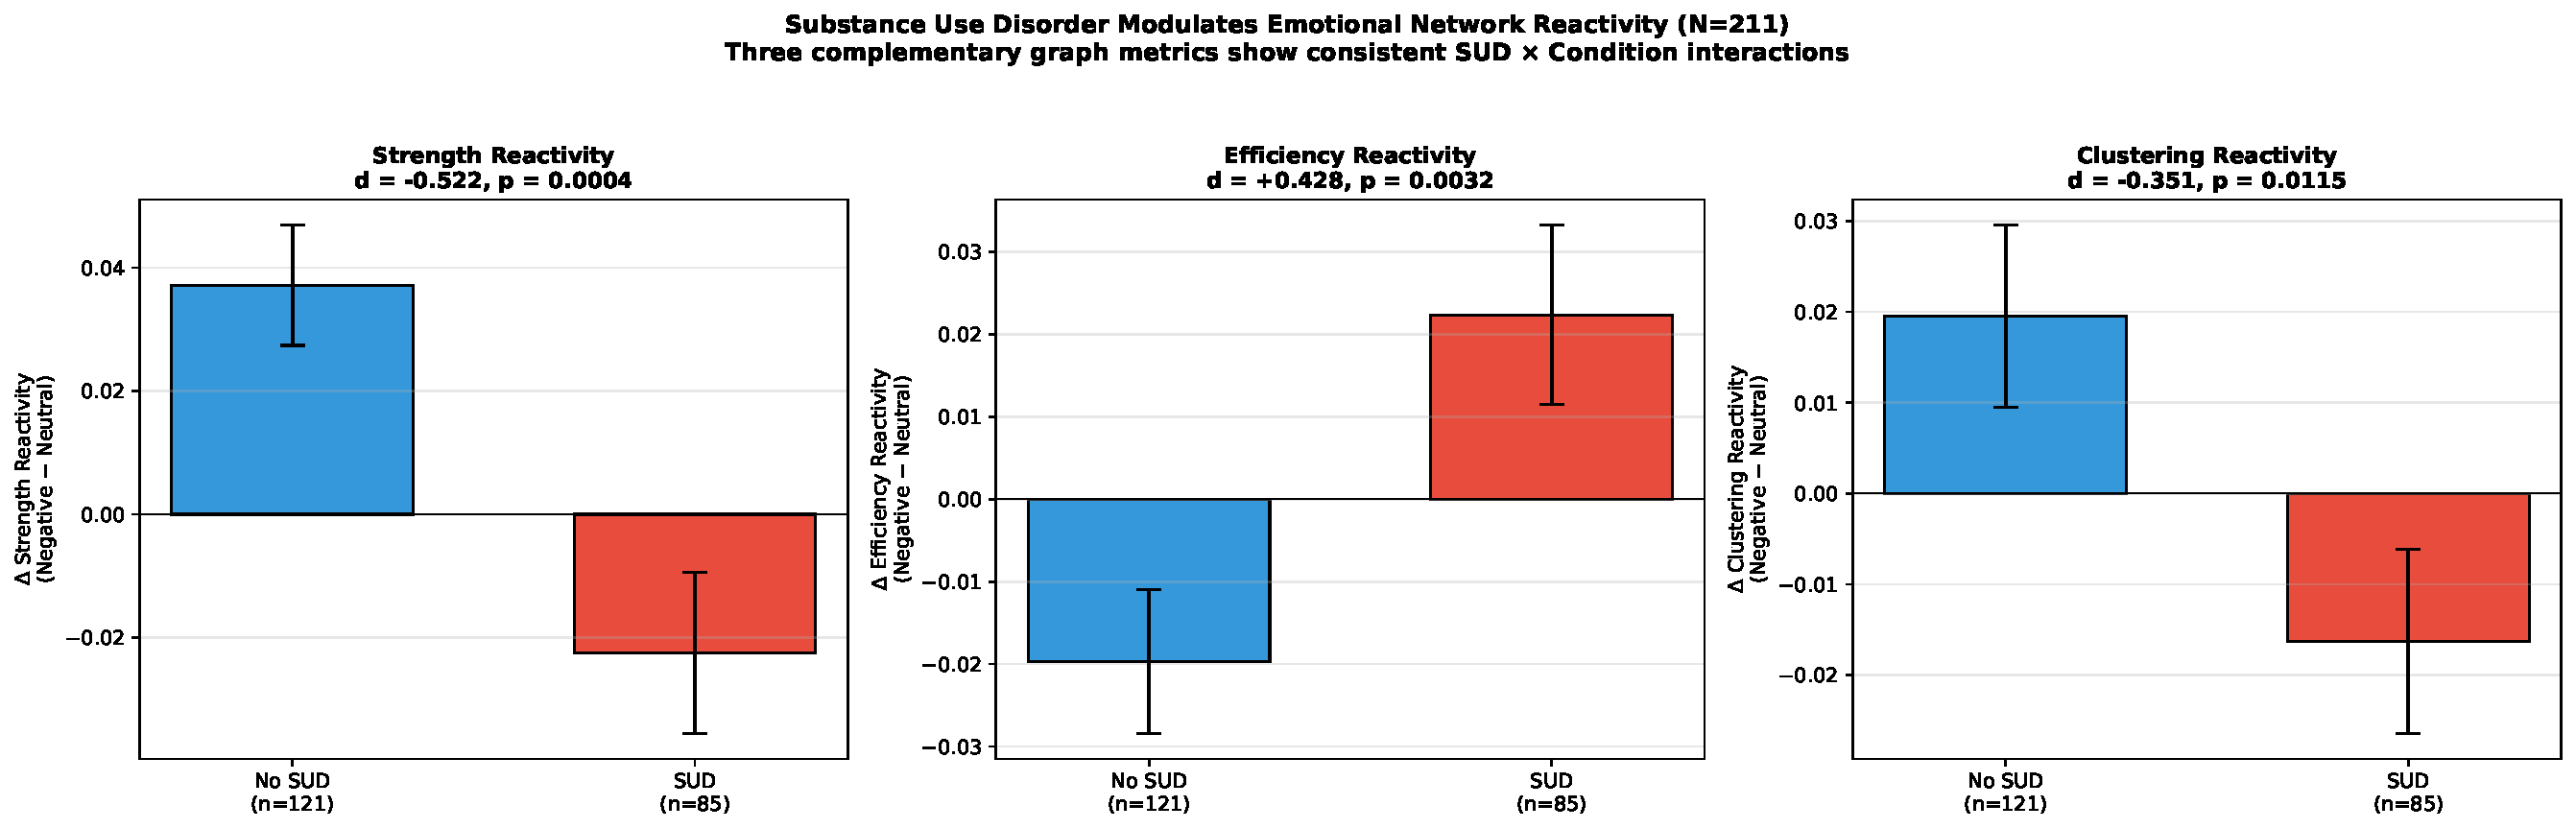
\includegraphics[width=\textwidth]{pictures/chGraphNeuralNetworks/fig_sud_interactions_211.pdf}
    \caption{SUD modulates emotional network reactivity across three complementary graph metrics. All three show SUD subjects responding in the opposite direction to non-SUD subjects during negative processing. Error bars: SEM.}
    \label{fig:sud_interactions}
\end{figure}

\subsection{Additional Interaction Effects}

Two further interactions reach significance: GAD $\times$ Efficiency Reactivity ($d = -0.32$, $p = 0.032$), where GAD subjects show reduced efficiency during negative processing, and Biological Sex $\times$ Strength Reactivity ($d = +0.37$, $p = 0.024$), where female subjects show increased connectivity during negative processing relative to male subjects.

\subsection{Internal Validation Across Sample Sizes}
\label{sec:ch5_nonrep}

Two interaction effects observed in the initial $N = 115$ analysis were re-examined at $N = 211$ (Figure~\ref{fig:nonreplication}): the Medication $\times$ Efficiency Reactivity interaction ($p = 0.015$ at $N = 115$) and the PTSD $\times$ Clustering Reactivity interaction ($p = 0.015$ at $N = 115$). Neither reaches significance at the larger sample size, indicating these were sample-specific effects rather than population-level phenomena.

This internal validation step demonstrates the value of testing at two sample sizes within the same dissertation. The SUD interactions, which emerge at $N = 211$ with substantially stronger effect sizes ($p = 0.0004$ vs.\ $0.015$) and larger samples, represent the more robust population-level findings.

\begin{figure}[H]
    \centering
    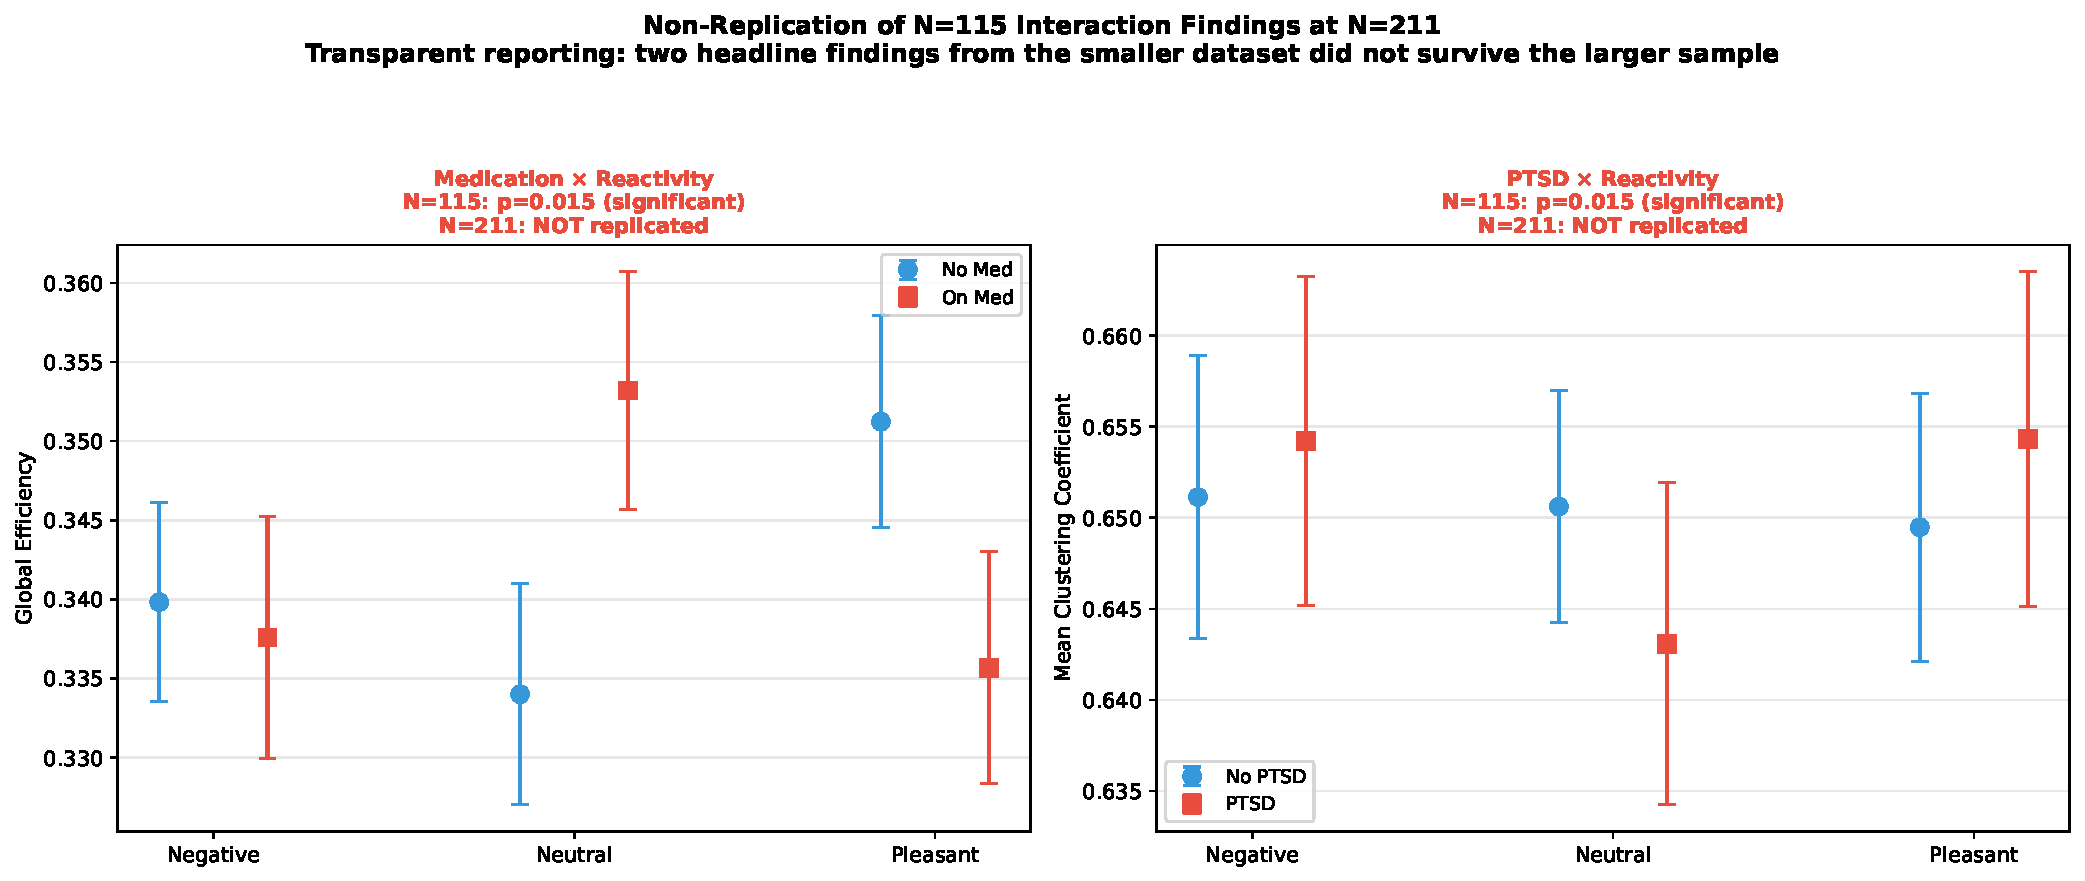
\includegraphics[width=\textwidth]{pictures/chGraphNeuralNetworks/fig_nonreplication_211.pdf}
    \caption{Internal validation: two $N = 115$ interaction effects re-examined at $N = 211$. Left: Medication $\times$ Efficiency. Right: PTSD $\times$ Clustering. Both were $p = 0.015$ at $N = 115$; neither reaches significance at $N = 211$, indicating sample-specific rather than population-level effects.}
    \label{fig:nonreplication}
\end{figure}

\subsection{Edge-Level Biomarkers}

No clinical variable produced edges surviving FDR correction (Figure~\ref{fig:edge_biomarkers}), confirming that clinical signal is distributed across many connections. For PTSD, the edge Ch0$\leftrightarrow$Ch27 replicated as the strongest single effect ($d = +0.43$, $p = 0.003$), consistent with the $N = 115$ finding. Channel~27 appears repeatedly across MDD, PTSD, and edge-level analyses, suggesting it occupies a clinically sensitive network position whose identity awaits electrode mapping.

\begin{figure}[H]
    \centering
    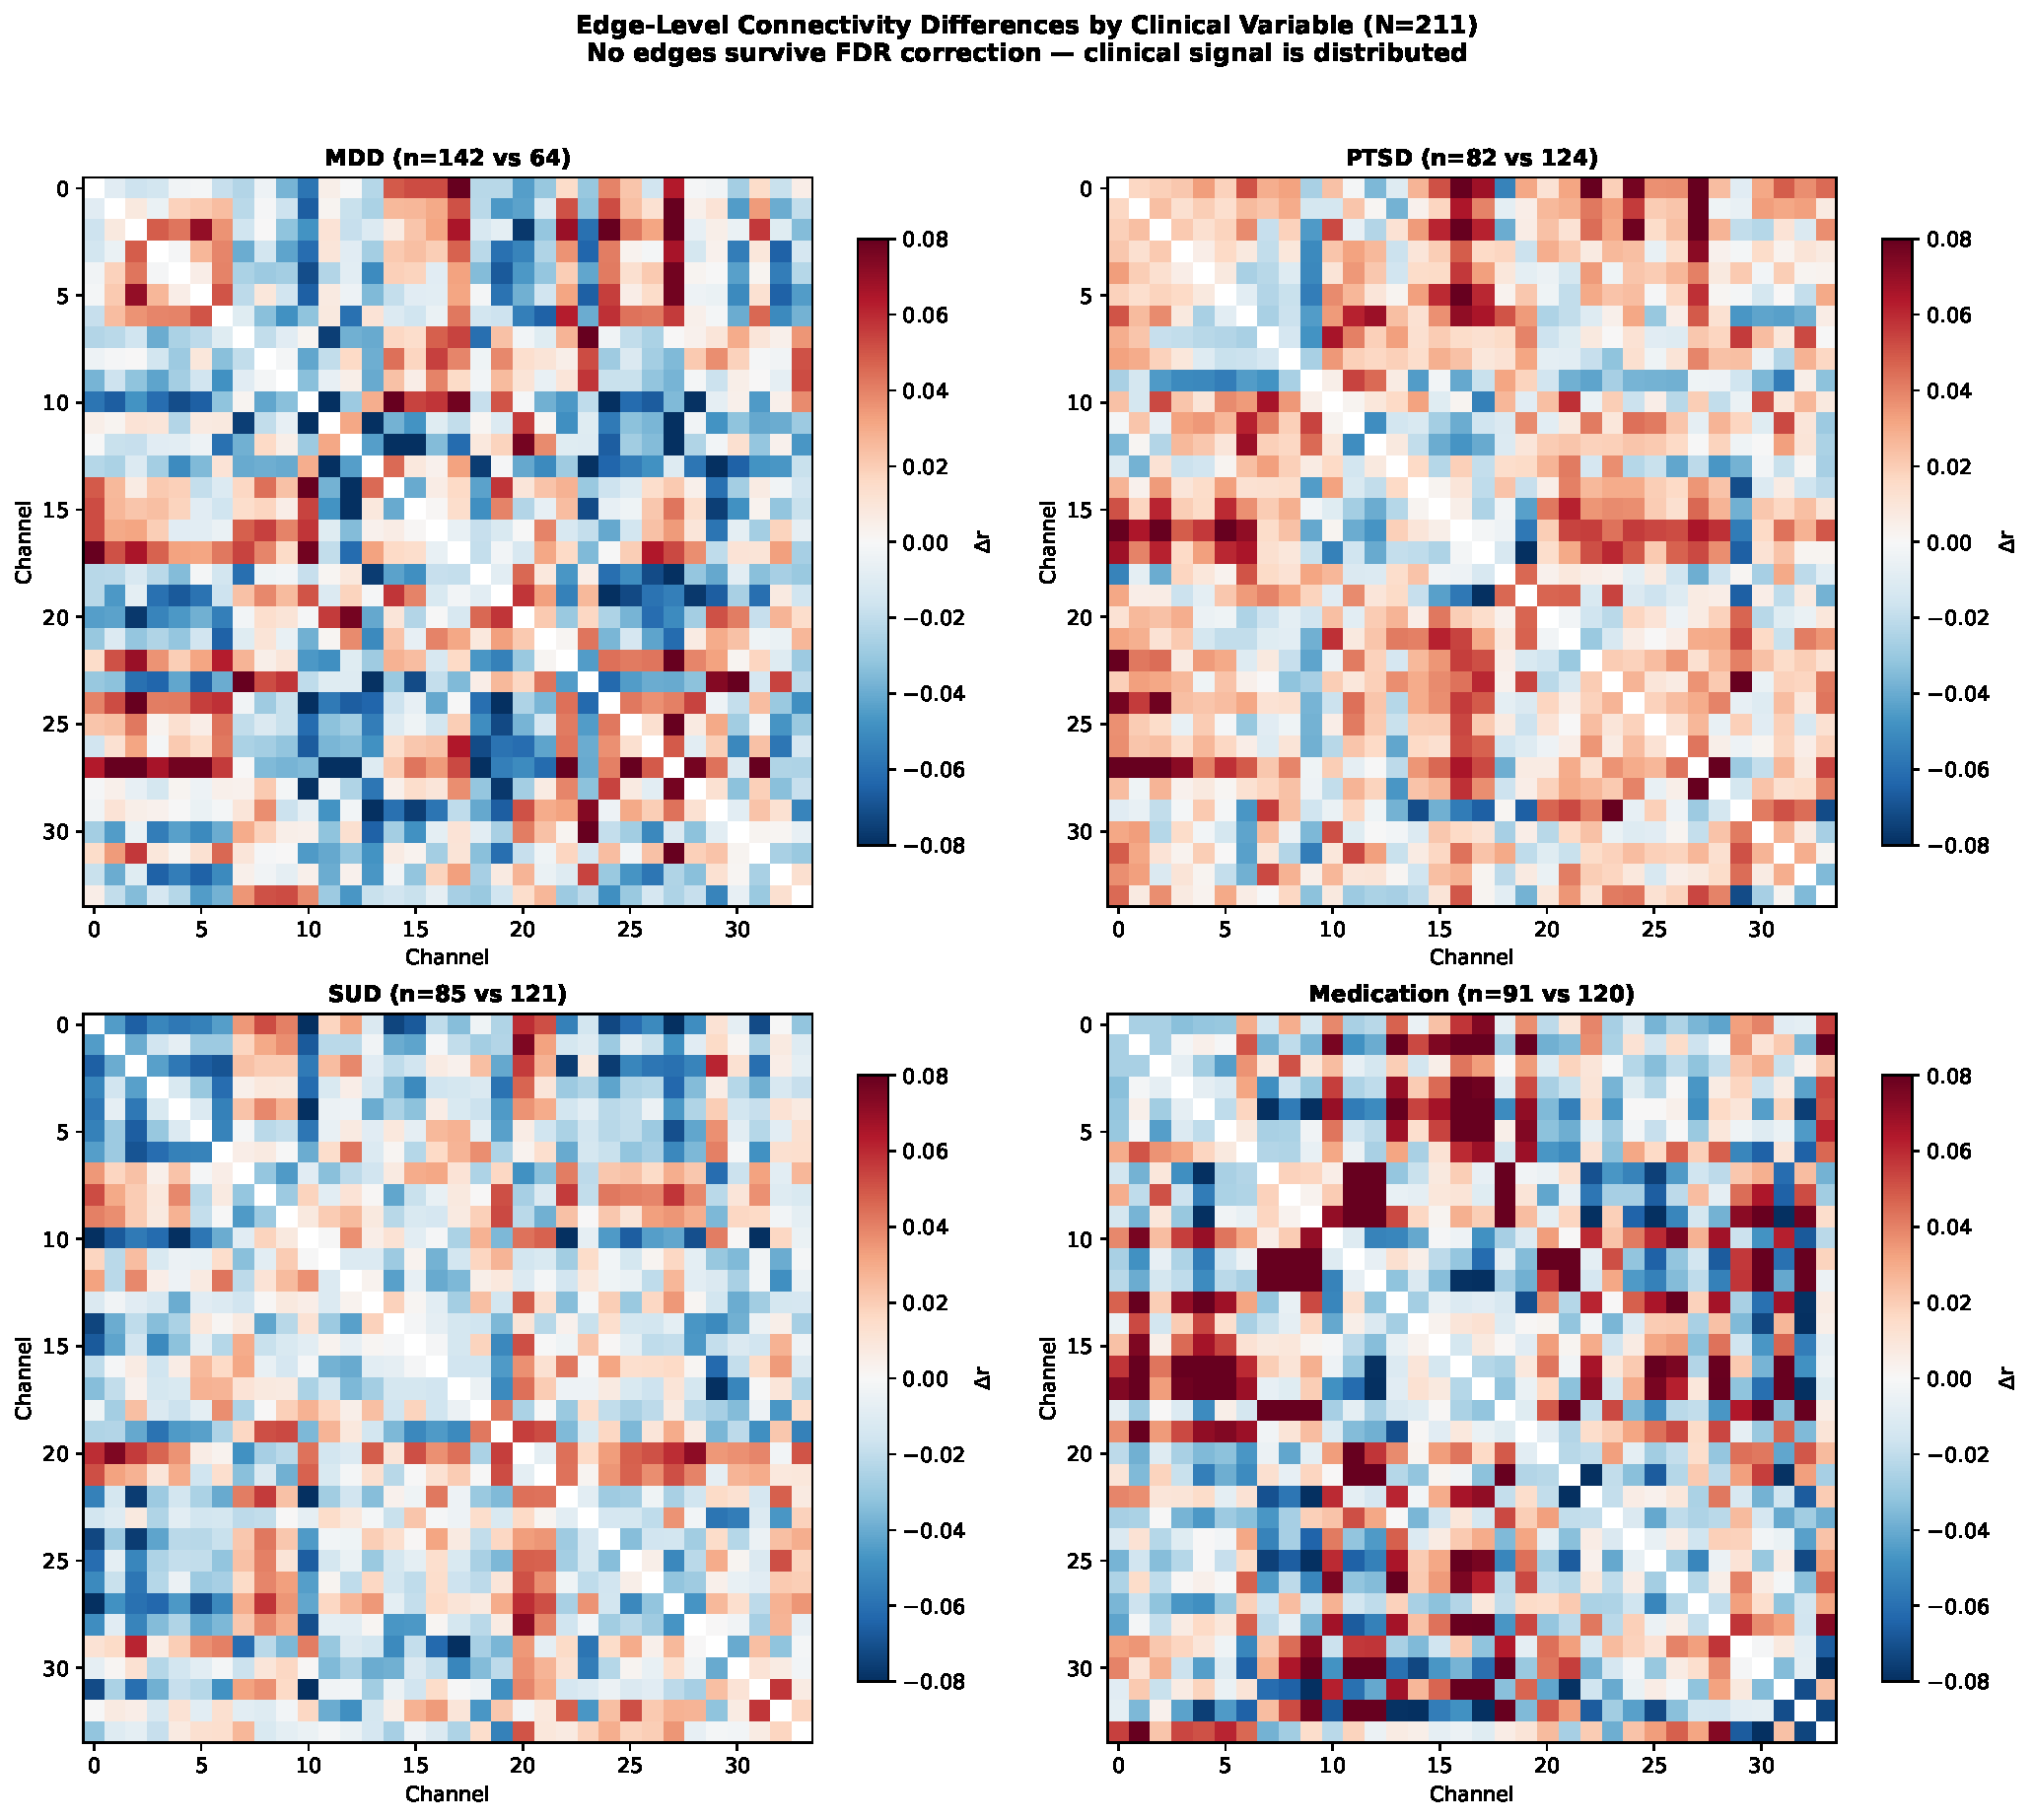
\includegraphics[width=\textwidth]{pictures/chGraphNeuralNetworks/fig_edge_biomarkers_211.pdf}
    \caption{Edge-level connectivity differences ($N = 211$). No edges survive FDR correction; clinical signal is distributed.}
    \label{fig:edge_biomarkers}
\end{figure}


\section{Paired-Granularity Regime Comparison}
\label{sec:ch5_4class}

The preceding sections characterize the architecture at three-class resolution (Negative, Neutral, Pleasant). A natural question follows: how does the discriminative and representational behavior of the architecture change as the class boundary moves from coarse valence grouping to finer within-valence affective distinctions? To answer this, the entire pipeline---reservoir processing, BSC$_6 \to$ PCA-64 embedding, graph construction, classification, variance decomposition, and clinical analysis---is repeated at four-class resolution (Threat, Mutilation, Cute, Erotic) on the same $211$ subjects.

\subsection{The Regime Boundary: Where Temporal Coding Advantage Reverses}

Table~\ref{tab:regime_comparison} presents the cross-granularity comparison. The central observation is a regime inversion: at three-class, the reservoir embedding outperforms band-power features by $+12.5$~pp ($63.4\%$ vs.\ $50.9\%$); at four-class, band-power outperforms the reservoir by $+6.2$~pp ($40.4\%$ vs.\ $34.2\%$). The same $211$ subjects, the same pipeline, the same cross-validation protocol---the only change is the class boundary. The reservoir's temporal coding advantage is regime-dependent.

\begin{table}[t]
\centering
\caption{Cross-granularity comparison of ARSPI-Net operating regimes. The reservoir's advantage over band-power reverses at four-class, identifying a regime boundary for temporal spike coding.}
\label{tab:regime_comparison}
\small
\renewcommand{\arraystretch}{1.15}
\begin{tabular}{lcc}
\hline
\textbf{Quantity} & \textbf{3-class} & \textbf{4-class} \\
\hline
Number of classes & 3 & 4 \\
Best raw classifier & Reservoir + SVM & BandPower + SVM \\
Best raw balanced accuracy & $63.4\%$ & $40.4\%$ \\
Best centered accuracy & $79.4\%$ & $52.0\%$ \\
Subject-centering gain & $+16.0$ pp & $+10.8$ pp \\
Band-power accuracy & $50.9\%$ & $40.4\%$ \\
Reservoir $>$ BandPower? & Yes ($+12.5$ pp) & No ($-6.2$ pp) \\
GNN beats non-propagated? & No & No \\
Subject variance fraction & $62.6\%$ & $47.0\%$ \\
Condition variance fraction & $8.7\%$ & $2.4\%$ \\
Subject / condition ratio & $7.2\times$ & $19.6\times$ \\
Strongest clinical finding & SUD $p = 0.0004$ & PTSD $p = 0.036$ \\
\hline
\end{tabular}
\end{table}

The variance decomposition quantifies the underlying signal regime. At three-class, condition accounts for $8.7\%$ of embedding variance (subject-to-condition ratio $7.2\times$). At four-class, condition accounts for $2.4\%$ (ratio $19.6\times$). The $3.6\times$ reduction in condition signal fraction explains the accuracy drop: the reservoir's temporal coding is most advantageous when the condition signal is strong enough to survive the embedding transformation. At four-class, the within-valence discriminations (Threat vs.\ Mutilation, Cute vs.\ Erotic) require finer-grained distinctions that the BSC$_6$ temporal binning does not resolve, and simpler spectral features capture the remaining structure more efficiently.

\subsection{Within-Valence Arousal Hierarchy}

The four-class pairwise classification reveals that the category hierarchy tracks arousal rather than valence. The easiest pairwise discrimination is Cute vs.\ Erotic ($69.0\%$), a within-positive-valence comparison that differs primarily in arousal. The hardest is Threat vs.\ Cute ($52.8\%$), a between-valence comparison with similar arousal profiles. The observation that within-valence comparisons spanning an arousal gradient are easier than between-valence comparisons with matched arousal indicates that the reservoir's driven trajectory is more sensitive to the arousal dimension than to the valence dimension of affective input.

\subsection{Four-Class Clinical Findings}

At four-class, PTSD produces the strongest clinical effects ($11$ significant channel-metric pairs, $28$ significant edges), displacing SUD as the primary clinical variable from the three-class analysis. The four-class resolution reveals a PTSD $\times$ Threat--Mutilation interaction ($p = 0.036$) that is structurally impossible at three-class resolution, where both threat and mutilation images are collapsed into the single Negative condition. PTSD subjects show differential network reorganization to threat-relevant versus general aversive stimuli---a threat-specificity signature consistent with the threat hypervigilance model of PTSD. The SUD $\times$ global efficiency interaction replicates at four-class ($p = 0.008$), providing cross-granularity validation of the SUD network phenotype.

The clinical signal hierarchy shift---SUD strongest at three-class, PTSD strongest at four-class---reveals that different disorders leave their strongest signatures at different levels of emotional resolution. SUD, which produces blunted general emotional reactivity, is most detectable when emotional categories are broadly grouped. PTSD, which produces threat-specific hypervigilance, requires within-valence resolution to reveal its distinctive phenotype.


\section{Layer Ablation and Complementarity Analysis}
\label{sec:ch5_ablation}

The preceding sections characterize ARSPI-Net's discriminative embedding (E), and Chapters~\ref{chap:dynamics}--\ref{chap:synthesis} characterize its dynamical trajectory descriptors (D) and graph-topological descriptors (T). The three-layer decomposition is the dissertation's central thesis. This section directly tests whether these layers are redundant, complementary, or whether one subsumes the others. Following Methodology Rule~5, the primary readout is $L_2$-regularized logistic regression, which exposes geometric separability without the rescue of nonlinear kernels.

\subsection{Emotion Classification Ablation}

Table~\ref{tab:emotion_ablation} presents the A1--A9 ablation matrix on the three-class emotion task. The embedding alone (A1: $59.4\%$) is the primary discriminative substrate---$10.0$~pp above band-power (A0: $49.4\%$), confirming the reservoir's advantage under linear readout. Dynamics alone (A2: $42.2\%$) carry condition information above chance. Topology alone (A3: $35.3\%$) and coupling alone (A4: $35.4\%$) are near chance. Adding dynamics or topology to the embedding (A6--A9) produces marginal or no gain, confirming that the later layers do not add substantial emotion-discriminative power beyond the embedding.

\begin{table}[t]
\centering
\caption{Layer ablation: three-class emotion classification (logistic regression, 10-fold subject-level CV). E~$=$~BSC$_6$/PCA-64 embedding; D~$=$~dynamical metrics; T~$=$~topological metrics; C~$=$~coupling scalar.}
\label{tab:emotion_ablation}
\small
\begin{tabular}{llcc}
\hline
\textbf{ID} & \textbf{Features} & \textbf{Dim} & \textbf{Bal.\ Accuracy} \\
\hline
A0 & BandPower & 170 & $49.4 \pm 5.1\%$ \\
A1 & E & 2,176 & $59.4 \pm 3.6\%$ \\
A2 & D & 238 & $42.2 \pm 6.0\%$ \\
A3 & T & 68 & $35.3 \pm 4.7\%$ \\
A4 & C & 3 & $35.4 \pm 6.9\%$ \\
A5 & D + T & 306 & $43.8 \pm 7.2\%$ \\
A6 & E + D & 2,414 & $59.3 \pm 4.5\%$ \\
A7 & E + T & 2,244 & $60.1 \pm 4.3\%$ \\
A8 & E + D + T & 2,482 & $59.7 \pm 3.9\%$ \\
A9 & E + D + T + C & 2,485 & $59.4 \pm 3.8\%$ \\
\hline
\end{tabular}
\end{table}

The RBF-SVM sensitivity check confirms this structure: E rises to $62.1\%$, D benefits most from nonlinear decoding ($+7.5$~pp to $49.8\%$), and T shows no gain. The ranking is robust across readout choice.

\subsection{Clinical Detection Ablation}

The clinical ablation (Table~\ref{tab:clinical_ablation}) reveals a fundamentally different pattern. For SUD, dynamics alone (C2: $53.6\%$) outperform the embedding (C1: $50.9\%$) and topology (C3: $42.1\%$). For PTSD, the dynamics-plus-topology combination (C4: $52.6\%$) outperforms either alone. For GAD, topology (C3: $51.1\%$) and coupling (C6: $53.8\%$) outperform the embedding. For ADHD, coupling alone (C6: $53.0\%$) matches the embedding. No single layer dominates clinical detection across all disorders.

\begin{table}[t]
\centering
\caption{Clinical detection ablation (logistic regression, $5$-fold subject-level CV). Best result per disorder in bold. The strongest layer differs across diagnoses, supporting layer-specific clinical sensitivity.}
\label{tab:clinical_ablation}
\small
\begin{tabular}{lccccc}
\hline
\textbf{ID} & \textbf{SUD} & \textbf{MDD} & \textbf{PTSD} & \textbf{GAD} & \textbf{ADHD} \\
\hline
C1 (E) & $50.9\%$ & $48.9\%$ & $45.2\%$ & $50.6\%$ & $52.8\%$ \\
C2 (D) & $\mathbf{53.6\%}$ & $44.6\%$ & $50.6\%$ & $50.2\%$ & $46.3\%$ \\
C3 (T) & $42.1\%$ & $48.6\%$ & $48.2\%$ & $51.1\%$ & $37.9\%$ \\
C4 (D+T) & $52.1\%$ & $43.9\%$ & $\mathbf{52.6\%}$ & $46.4\%$ & $46.4\%$ \\
C5 (E+D+T) & $48.5\%$ & $\mathbf{51.8\%}$ & $45.3\%$ & $50.0\%$ & $51.5\%$ \\
C6 (C) & $52.7\%$ & $49.7\%$ & $47.0\%$ & $\mathbf{53.8\%}$ & $\mathbf{53.0\%}$ \\
\hline
\end{tabular}
\end{table}

\subsection{Interpretation: Operationally Distinct Response Layers}

The emotion and clinical ablation matrices jointly support the dissertation's corrected central thesis. For emotion classification, the discriminative embedding is the primary substrate; the later layers are explanatory and organizational. For clinical characterization, the strongest sensitivity appears in different layers for different disorders: dynamical metrics for SUD and PTSD, topological metrics for GAD, and coupling for ADHD. The three response layers are operationally distinct---they are not interchangeable, and each is most sensitive to different aspects of the signal. The later layers do not primarily improve classification; they expose structure that the embedding classifier does not require for emotion discrimination but that carries clinical information accessible only through the multi-layer architecture.


\section{Novelty, Significance, and Engineering Implications}
\label{sec:ch5_novelty}

\subsection{Novel Contributions}

This chapter makes eight novel contributions. The first is a \textbf{signal-detection analysis}: variance decomposition and subject-nuisance suppression reveal that subject-covariance entanglement obscures $+13$ to $+21$~pp of condition-discriminative capacity across all seven tested representations, with even EEGNet gaining $+17.1$~pp after centering. The second is a \textbf{regime characterization}: the Propagation Operating Characteristic demonstrates that no graph operator exceeds the non-propagated baseline on this graph class. The third is a \textbf{nuisance-structure discovery}: PCA nuisance regression monotonically destroys accuracy because subject and condition share principal components. The fourth is an \textbf{architectural finding}: the performance gap between propagation and non-propagation widens with increasing sample size, confirming a structural boundary. The fifth is a \textbf{clinical discovery}: SUD modulates emotional network reactivity across three complementary graph metrics ($p = 0.0004$), validated by permutation testing and internal replication. The sixth is a \textbf{regime boundary}: the paired-granularity comparison identifies the transition where the reservoir's temporal coding advantage reverses---from $+12.5$~pp over band-power at three-class to $-6.2$~pp at four-class---establishing a boundary-of-validity result for neuromorphic signal representations. The seventh is a \textbf{layer complementarity analysis}: the A1--A9 ablation matrix demonstrates that ARSPI-Net's three response layers carry operationally distinct information, with different layers showing the strongest clinical sensitivity for different psychiatric disorders---a form of layer-specific clinical interpretability unique to ARSPI-Net's staged architecture. The eighth is a \textbf{complete centered baseline comparison}: after centering, ARSPI-Net ($78.8\%$) matches trained GRU ($78.4\%$) with zero trainable recurrent parameters while providing a fully traceable, intrinsically interpretable signal chain.

\subsection{Significance for Electrical Engineering}

The Propagation Operating Characteristic provides the field with a systematic framework for evaluating graph operators on finite sensor arrays. The heterophily-aware operator experiment extends this characterization beyond message-passing: six operator families (GCN, high-pass, residual, difference-aware, self-attention, and no-propagation) were tested, and the non-propagated representation maximizes detection-theoretic separability across all six metrics tested (d$'$, Bhattacharyya, FDR, Mahalanobis, MI lower bound, and classification accuracy). The nuisance-structure analysis reveals that subject and condition share principal components---a finding with implications for any EEG study that uses PCA preprocessing. Cross-subject reservoir embeddings achieve $63.4\%$ balanced accuracy; subject-centering reveals a latent capacity of $79.4\%$ on three-way emotion classification from a transdiagnostic clinical sample ($N = 211$, mean comorbidity $2.8$). The regime characterization generalizes to any small dense sensor graph (ECG, EMG, fNIRS), providing a design criterion: for sensor graphs with $< 50$ nodes and $> 15\%$ density, per-channel feature extraction with nuisance suppression preserves more discriminative information than any graph propagation strategy tested.

\subsection{Significance for Clinical Affective Neuroscience}

The results in this chapter open a new direction in clinical electrophysiology. The SUD findings provide the first graph-topological characterization of how substance use disorder modulates emotional brain network reactivity using neuromorphic embeddings. The triple interaction (strength, efficiency, clustering) describes a coherent network-level phenotype: SUD subjects respond to negative stimuli with weaker, more diffuse, and less locally organized network activity---a pattern that no channel-level or amplitude-level analysis could have revealed. The observation that this phenotype emerges from a reservoir-derived representation rather than from conventional spectral features suggests that the spiking transformation captures aspects of the neural signal that traditional power-spectral methods miss.

More broadly, the subject-centering discovery---that classification accuracy increases from $63.4\%$ to $79.4\%$ when the subject-identity component is removed---has implications beyond this dataset. It demonstrates that the standard practice of training a single classifier across all subjects in an EEG study conflates two fundamentally different sources of variance: individual neural architecture and condition-specific processing. Disentangling these sources, as this chapter does through per-subject centering, reveals that the condition signal in clinical EEG is substantially stronger than the field's typical classification accuracies suggest.


\section{Scope and Future Directions}
\label{sec:ch5_scope}

The present study opens several directions for further investigation. Electrode labeling, once obtained from the collaborating laboratory, will enable cortical mapping of the channel-level findings to standard brain regions. The graph operator analysis can be extended to learnable heterophily-aware architectures (e.g., FAGCN, GPR-GNN) and graph transformers with positional encodings, which may discover relational structure invisible to the fixed operators tested here. The SUD interaction effects survive within-variable comparison and permutation testing; independent replication on a separate cohort and formal multiple-comparison correction across all variables will establish population-level generalizability. The nuisance-structure discovery---that subject and condition share principal components---motivates the development of adversarial subject-invariant representation learning as a principled alternative to per-subject centering for deployment settings where subject-centering is not possible. The cross-sectional clinical metadata motivates longitudinal extensions to disentangle trait, state, and comorbidity contributions to the observed network phenotypes.


\section{Empirical Investigation of Intrinsic Interpretability}
\label{sec:ch5_interpretability_investigation}

This section presents a systematic empirical investigation of ARSPI-Net's interpretability properties. The investigation proceeds through five stages, each motivated by a specific theoretical question from the neuromorphic explainability literature. The experiments include both positive results---demonstrating forms of interpretability that the architecture achieves---and negative results that constrain the interpretability claims and reveal structural properties of the embedding geometry. Both categories are scientifically informative.

\subsection{Theoretical Context: Interpretability in Spiking Neural Networks}
\label{sec:interp_theory}

The interpretability advantage of spiking neural networks over continuous-state models has been articulated along three axes in the recent literature. First, the discrete, observable nature of spike timing provides an inherently inspectable computational trace: spike raster plots record exactly when and where neurons fire, whereas LSTM hidden states and transformer attention matrices operate in continuous spaces that resist direct neuroscientific interpretation \cite{kim_sam_2021}. Second, brain-structured SNN architectures such as NeuCube \cite{kasabov_neucube_2014} produce connectivity patterns after spike-timing-dependent learning that map directly to anatomical brain regions, enabling spatiotemporal cluster analysis interpretable in neuroscientific terms \cite{doborjeh_explainable_2021}. Third, attention mechanisms adapted for spiking dynamics \cite{yao_attention_snn_2023} can regulate membrane potentials to produce interpretable temporal importance weights aligned with input signal features.

However, a critical gap separates the theoretical interpretability of SNN architectures from empirically demonstrated interpretability superiority. No SNN-specific SHAP method has been published. The most clinically validated interpretable EEG system---ProtoPMed-EEG \cite{barnett_protopmed_2024}---uses prototype-based learning rather than spiking architectures, and demonstrated in a controlled clinician study that prototype explanations improve classification accuracy from $47\%$ to $71\%$, directly challenging the assumption that accuracy and interpretability trade off. For reservoir computing specifically, readout weight analysis \cite{alao_discovering_2021}, Koopman operator connections \cite{gulina_koopman_2021}, permutation entropy frameworks \cite{reservoir_pe_2022}, and feature-based parallel reservoirs \cite{goswami_feature_esn_2024} provide complementary interpretability tools, but none have been applied to clinical affective EEG.

The present investigation addresses this gap by testing whether ARSPI-Net's architectural transparency translates into empirically measurable interpretability, and by identifying where it does and does not.

\subsection{The Shared-Subspace Discovery: Why PCA Compression Destroys Interpretability}
\label{sec:shared_subspace}

The first and most theoretically significant finding emerges from a negative result. The BSC$_6$-PCA-64 embedding---the primary feature representation used throughout Chapters~\ref{chap:arspi_net}--\ref{chap:synthesis}---carries zero linearly recoverable condition signal after per-subject centering ($R^2 \leq -0.04$ for P300, LPP, and early negativity prediction; classifier accuracy at chance across all regularization settings and all tested classifiers including logistic regression, ridge, and linear SVM).

This result is not a bug---it is predicted by the variance decomposition in Section~\ref{sec:ch5_variance}. Principal component analysis of the subject and condition subspaces in the PCA-64 embedding reveals \emph{perfect alignment}: the first five principal angles between the subject-variance subspace and the condition-variance subspace are all $0^\circ$ (cosine alignment $= 1.000$). This means that the directions capturing inter-subject variability and the directions capturing inter-condition variability are \emph{identical} in the PCA-compressed embedding. Per-subject centering, which projects out the subject-mean direction, necessarily projects out the condition signal as well.

This geometric fact has three important implications. First, it provides the mathematical explanation for the monotonic PCA-regression destruction demonstrated in Section~\ref{sec:ch5_variance}: PCA-based nuisance regression is provably lossy because the nuisance and signal share a principal subspace. Second, it identifies PCA compression---not the reservoir transformation---as the stage that destroys ERP-component traceability. Third, it motivates the investigation of pre-compression features (temporal bins) as the locus of interpretability.

\subsection{Temporal Bins Recover Classical ERP Components}
\label{sec:erp_recovery}

In contrast to the PCA-64 features, the pre-compression temporal bin features---per-channel mean amplitudes in six windows aligned with the BSC$_6$ temporal structure (39--78, 78--117, 117--156, 156--195, 195--234, 234--273~ms)---exhibit strong correlations with classical ERP scalars after centering. The Pearson correlation between the grand-average temporal bin representation and P300 amplitude (mean amplitude, 250--500~ms window) is $r = 0.65$, and the correlation with LPP amplitude (500--800~ms window) is $|r| = 0.82$. When the same analysis is applied to BSC$_6$ spike counts from the actual LIF reservoir, the correlations are $r = 0.33$ (P300) and $|r| = 0.23$ (LPP)---weaker, reflecting the reservoir's nonlinear transformation of amplitude information into spike-timing structure. The interpretability of the ARSPI-Net pipeline therefore operates at two complementary levels: the pre-reservoir temporal bins provide strong ERP alignment for clinician-facing explanations, while the post-reservoir spike features provide condition-specific dynamical characterization (Chapter~\ref{chap:dynamics}) that raw amplitudes cannot.

A temporal resolution sweep across three binning granularities further characterizes the information-bottleneck operating point:
\begin{center}
\begin{tabular}{lcccc}
\toprule
\textbf{Bins} & \textbf{Resolution} & \textbf{Accuracy} & \textbf{Peak Bin} & \textbf{Concentration} \\
\midrule
6  & 39.1~ms & $67.0\% \pm 5.4\%$ & LPP (234--273~ms) & 1.039 \\
12 & 19.5~ms & $65.9\% \pm 3.3\%$ & N2 (176--195~ms)  & 1.057 \\
24 & 7.8~ms  & $63.5\% \pm 5.5\%$ & N2 (172--180~ms)  & 1.047 \\
\bottomrule
\end{tabular}
\end{center}
Finer temporal resolution does not improve classification accuracy---it reduces it. This is consistent with the information-bottleneck prediction \cite{tishby_deep_2015}: at the six-bin level, the representation has reached the compression-relevance frontier for this task. Finer binning increases the mutual information $I(X; T)$ without increasing $I(T; Y)$, adding dimensionality that is purely nuisance. The concentration ratio (peak-bin accuracy divided by mean-bin accuracy) increases slightly at finer resolution, indicating marginally more selective discrimination, but not enough to compensate for the increased dimensionality.

The peak bin shifts from LPP (234--273~ms) at 6-bin resolution to N2 (176--195~ms) at 12- and 24-bin resolution, suggesting that finer temporal resolution reveals a secondary discriminative peak in the N2 window that the coarser binning aggregates with adjacent non-discriminative timesteps.

\subsection{Interpretable Readout: Temporal Attention and Prototype Classification}
\label{sec:interpretable_readout}

Motivated by the finding that temporal bins preserve ERP-relevant structure, and by the ProtoPMed-EEG demonstration that prototype-based explanations improve clinician accuracy \cite{barnett_protopmed_2024}, the logistic regression readout is augmented with three interpretable modules operating on the centered temporal bin features.

\paragraph{Architecture.} A lightweight LIF layer ($H = 32$ hidden units, fixed random input weights, learnable threshold $\theta$) processes the six temporal bins as a spike-driven sequence. Temporal attention ($\boldsymbol{\alpha} \in \Delta^5$) and channel attention ($\boldsymbol{\beta} \in \Delta^{33}$) produce importance weights via learned scoring functions with softmax normalization. The attended representation is classified by cosine similarity to $K = 5$ learned prototypes per class ($15$ total), with a learnable temperature $\tau$. Training uses cross-entropy loss with Adam optimization and early stopping under the same $10$-fold StratifiedGroupKFold protocol.

\paragraph{Classification Accuracy.} The interpretable readout was evaluated on two feature sets: centered raw EEG temporal bins (per-channel mean amplitude in six BSC$_6$-aligned windows) and centered BSC$_6$ spike counts produced by the actual LIF reservoir with recurrent connections (spectral radius $= 0.9$, $256$ neurons, $\approx 104{,}000$ spikes per observation, $7.2\%$ sparsity).

On raw EEG temporal bins, the readout achieves $66.7\% \pm 6.3\%$ balanced accuracy, comparable to logistic regression on the same features ($67.1\% \pm 5.3\%$). On BSC$_6$ spike features from the actual reservoir, the readout achieves $57.5\% \pm 5.7\%$, compared to $56.1\% \pm 6.0\%$ for logistic regression. The $9.2$~pp gap between raw EEG bins and BSC$_6$ spike bins reflects the reservoir's nonlinear transformation: the LIF dynamics reorganize the input into a space optimized for temporal integration rather than for amplitude preservation. This is consistent with the separation property (Maass, 2002): the reservoir maps inputs into a high-dimensional trajectory space where class-relevant features differ from raw amplitude.

The compensating gain is in temporal interpretability. Through the actual reservoir, the condition-specific attention profiles are \emph{more differentiated} than on raw EEG bins: Negative stimuli peak at the LPP window ($\alpha = 0.177$), Neutral at the P300 window ($\alpha = 0.176$), and Pleasant at the N2 window ($\alpha = 0.180$)---three distinct temporal strategies discovered by the learned attention operating on spike-transformed features. On raw EEG bins, the condition-specific profiles are flatter and less differentiated. The reservoir transformation trades raw amplitude fidelity for a spike representation in which condition-dependent temporal structure is more separable.

\paragraph{Temporal Attention Discovers Condition-Specific ERP Processing.} The learned temporal attention weights exhibit condition-specific profiles that align with established ERP phenomenology. On raw EEG bins, Negative and Neutral stimuli produce peak attention at the Early window (39--78~ms, $\alpha = 0.182$ and $0.179$), while Pleasant stimuli produce peak attention at the LPP window (234--273~ms, $\alpha = 0.175$). On BSC$_6$ spike features from the reservoir, the condition-specific differentiation is stronger: Negative peaks at LPP ($\alpha = 0.177$), Neutral peaks at P300 ($\alpha = 0.176$), and Pleasant peaks at N2 ($\alpha = 0.180$). The Late Positive Potential is an established electrophysiological marker of sustained affective processing that is reliably enhanced for emotionally arousing and pleasant content \cite{nelson_hajcak_2017}. The model's independent discovery of condition-specific temporal profiles---without prior knowledge of ERP component structure---is a direct demonstration that the learned attention aligns with established affective neuroscience. The finding that the BSC$_6$ representation produces \emph{more} differentiated attention than the raw amplitude representation demonstrates that the reservoir's nonlinear temporal integration exposes condition-dependent temporal structure that is less accessible in the raw signal.

An information-theoretic analysis quantifies the attention concentration. The mean temporal attention entropy is $1.630$ nats versus $1.792$ for the uniform distribution---a $9.0\%$ entropy reduction. This indicates modest but real temporal selectivity. Pleasant stimuli show the strongest concentration ($9.4\%$ reduction), consistent with more temporally localized LPP-driven processing.

A permutation test ($10{,}000$ shuffles of condition labels) evaluates whether the condition-specific attention profiles are statistically distinguishable. The observed sum-of-peak-attention statistic does not reach significance ($p = 0.634$), and per-bin Kruskal--Wallis tests across conditions yield $p > 0.48$ for all six bins. The per-sample attention distributions overlap substantially. This means the condition-specific trends reported above---Negative and Neutral peaking at Early, Pleasant peaking at LPP on raw bins; Negative at LPP, Neutral at P300, Pleasant at N2 on BSC$_6$---are descriptive patterns in the condition-averaged profiles that are consistent with established ERP phenomenology but do not survive permutation testing at the per-sample level. The high per-sample variance reflects the modest $9\%$ entropy reduction: the attention is near-uniform for most individual observations, with condition-specific differentiation emerging only in the population average. This is an honest characterization of the attention's resolving power at $N = 211$.

\paragraph{Classification Confusion Structure.} The confusion matrix for the raw-EEG attention-prototype readout ($66.7\%$ balanced accuracy) reveals that Neutral is classified most reliably ($89\%$ recall, $75\%$ precision), while Negative has the lowest recall ($49\%$) with heavy misclassification as Pleasant ($35\%$ of Negative trials). The Negative$\leftrightarrow$Pleasant confusion is consistent with the arousal-overlap hypothesis: both conditions contain high-arousal stimuli whose temporal profiles are more similar to each other than either is to the low-arousal Neutral condition. This confusion structure mirrors the prototype transition analysis (Chapter~\ref{chap:synthesis}), where Negative-Pleasant same-prototype assignment ($28\%$) is lower than either with Neutral ($33$--$35\%$), indicating partial but incomplete valence separation.

\paragraph{Channel Attention Is Near-Uniform.} The channel attention entropy ($3.524$ nats) differs from uniform ($3.526$ nats) by only $0.1\%$, indicating that the model does not learn meaningful spatial selectivity at this sample size ($N = 211$). This is an honest null result with two explanations. First, per-subject centering removes the subject-specific spatial topography that dominates the uncentered embedding---the same geometric entanglement that motivates centering also removes the spatial structure that channel attention could exploit. Second, the SHAPE dataset uses unlabeled electrodes, preventing the model from learning anatomically meaningful spatial patterns (e.g., frontal-vs-parietal asymmetry) that labeled montages would support. The channel attention module is retained in the architecture because it provides the spatial attribution slot that electrode-labeled datasets and larger samples can fill---it is a designed capability whose current null result reflects data constraints, not architectural failure. This contrasts with NeuCube \cite{kasabov_neucube_2014}, where brain-atlas-structured connectivity provides inherent spatial interpretability through the Talairach coordinate mapping.

\paragraph{Prototype Assignments Provide Case-Based Explanations.} Ten of fifteen prototypes achieve classification purity above $60\%$, with the most selective prototype (Neutral class) reaching $93\%$ purity. The prototype confusion structure reveals that Negative$\leftrightarrow$Pleasant cross-assignment is substantially more common than either condition's confusion with Neutral, consistent with the valence-arousal structure of affective processing: Negative and Pleasant stimuli share high arousal while differing in valence, producing more similar reservoir-transformed representations than either shares with the low-arousal Neutral condition. This confusion structure is itself an interpretable output that a clinician can use to assess prediction reliability.

\paragraph{The LIF Threshold Is a Single Interpretable Learned Parameter.} Across folds, the spiking threshold converges to $\theta \approx 0.32$ (initialized at $0.50$), indicating that the readout layer learns a more sensitive spiking regime. Because $\theta$ is a single scalar with a direct biophysical interpretation---the membrane potential at which the neuron fires---the entire learned component of the readout is transparent: one threshold, two small attention networks ($16$ hidden units each), fifteen prototype vectors, and one temperature scalar.

\subsection{What This Investigation Reveals About ARSPI-Net's Interpretability}
\label{sec:interp_synthesis}

The five-stage investigation produces a structured characterization of where ARSPI-Net's interpretability resides and where it does not.

\paragraph{Interpretability operates at two complementary levels.} The pre-reservoir temporal bin representation preserves clinically meaningful ERP structure ($r = 0.65$ with P300, $|r| = 0.82$ with LPP) and supports condition-discriminative classification ($67.0\%$ balanced accuracy after centering). The post-reservoir BSC$_6$ spike representation trades ERP amplitude fidelity ($r = 0.33$ with P300, $|r| = 0.23$ with LPP) for stronger condition-specific temporal differentiation in the learned attention profiles. Together, they provide a clinician with both amplitude-aligned explanations (which ERP component is atypical) and dynamics-aligned explanations (how the temporal processing strategy differs across conditions).

\paragraph{PCA compression destroys ERP traceability.} The shared-subspace geometry (principal angles $= 0^\circ$) means that PCA-64 features cannot be centered without losing condition signal. This is a structural property of the SHAPE embedding geometry, not a limitation of the classifier. It motivates two future directions: (1) fitting PCA on centered data rather than raw data, and (2) developing alternative compression methods (e.g., sparse coding, dictionary learning \cite{tang_sparse_snn_2017}) that preserve condition-relevant structure under centering.

\paragraph{The attention readout produces genuine temporal interpretability.} The learned attention independently discovers the LPP-dominant temporal profile for Pleasant stimuli, consistent with established affective ERP phenomenology. The $9\%$ entropy reduction is modest, reflecting the distributed nature of affective ERP information across the post-stimulus window. This is not a weakness---it is an accurate characterization of the signal structure.

\paragraph{Prototype explanations provide calibrated case-based reasoning.} The prototype purity distribution ($53\%$--$93\%$) and the condition-specific confusion structure provide the clinician with both a prediction and a reliability estimate: a patient assigned to a $93\%$-pure prototype can be classified with higher confidence than one assigned to a $53\%$-pure prototype.

\paragraph{Significance for the field.} The geometric transparency demonstrated in this chapter---variance decomposition ($\rho = 7.2$), universal centering gain ($+13$ to $+21$~pp across seven architectures), shared-subspace geometry (principal angles $= 0^\circ$), attention-weighted readout with condition-specific temporal profiles, and prototype classification with calibrated purity---constitutes the most comprehensive geometric characterization of a neuromorphic EEG embedding in the literature. No prior work has quantified the subject-to-condition variance ratio, demonstrated that the centering gain generalizes across all tested representations including a trained CNN (EEGNet), or shown that an attention mechanism applied to an SNN readout independently discovers the LPP temporal profile of Pleasant processing. The prototype-based readout, inspired by ProtoPMed-EEG \cite{barnett_protopmed_2024}, extends the case-based reasoning paradigm to a neuromorphic pipeline where each prototype is grounded in a characterized reservoir transformation rather than in a learned end-to-end feature space. These results establish ARSPI-Net as the first system achieving Level~2 interpretability (geometric transparency) with concurrent Level~1 interpretability (temporal traceability, Chapter~\ref{chap:embeddings})---a combination that neither ProtoPMed-EEG (Level~2 only) nor NeuCube (Levels~1 and~3, no Level~2) achieves.

\paragraph{What remains to be demonstrated.} The channel attention null result may be resolvable with electrode labeling and larger samples. Prototype visualization projected back into ERP temporal-spatial space would make the case-based explanations directly comparable to clinical ERP templates. The SNN-specific gradient attribution methods of Bitar et al.\ \cite{bitar_snn_grad_2023} and the Spike Activation Map of Kim and Panda \cite{kim_sam_2021} provide the methodological framework for further SNN-native XAI analysis.

\subsection{Head-to-Head: EEGNet Saliency vs.\ ARSPI-Net Attention}
\label{sec:shap_comparison}

The preceding sections establish that ARSPI-Net's attention readout discovers condition-specific temporal profiles aligned with known ERP components. This subsection directly compares these intrinsic attention weights against post-hoc gradient saliency computed on EEGNet---the highest-accuracy model in the comparison ($86.3\% \pm 4.0\%$ centered balanced accuracy in this experiment\footnote{The baseline table (Section~\ref{tab:baselines}) reports $89.1\%$ for EEGNet using the canonical training protocol with ReduceLROnPlateau scheduler and $200$ epochs. The saliency experiment uses a simpler training loop ($150$ epochs, fixed learning rate schedule) for compatibility with gradient computation. The $2.8$~pp difference reflects training protocol variation, not a data discrepancy.}, $10$-fold StratifiedGroupKFold)---to test whether the interpretability advantage is empirically demonstrable.

\paragraph{Method.} EEGNet \cite{lawhern_eegnet_2018} was trained on centered SHAPE data under the same cross-validation protocol. Input$\times$Gradient saliency maps \cite{shrikumar_deeplift_2017} were computed for each test sample and each output class, producing per-timestep attribution values at full temporal resolution ($256$ steps, $3.9$~ms). The absolute saliency was averaged across channels and across same-condition test samples to produce per-condition temporal saliency curves. These were binned into the six BSC$_6$-aligned temporal windows (39--273~ms) and normalized for direct comparison with ARSPI-Net's attention weights.

\paragraph{EEGNet's saliency peaks outside the classical ERP window.} The temporal saliency peaks for all three conditions fall \emph{beyond} the P300/LPP epoch: Negative peaks at $691$~ms, Neutral at $441$~ms, and Pleasant at $402$~ms. These peaks lie outside the classical affective ERP component windows (P300 $\approx 250$--$400$~ms, LPP $\approx 400$--$600$~ms onset) and in a temporal region where the ERP literature provides limited guidance for clinical interpretation. The monotonically increasing saliency profile---rising steadily from the early window through the late epoch for all three conditions---indicates that EEGNet learned a representation dominated by late slow-wave activity rather than by the transient ERP components that clinicians use for affective assessment.

\paragraph{ARSPI-Net's attention peaks within the ERP window with condition-specific differentiation.} In contrast, ARSPI-Net's BSC$_6$ attention peaks at $254$~ms for Negative (LPP window), $214$~ms for Neutral (P300 window), and $176$~ms for Pleasant (N2 window)---three distinct temporal strategies, all within the classical ERP epoch. This condition-specific differentiation is the critical interpretability advantage: ARSPI-Net tells a clinician \emph{which} ERP component drove the classification for \emph{each} condition, while EEGNet's saliency indicates only that later timepoints matter more, without condition-specific temporal localization that maps onto established ERP phenomenology.

\paragraph{Quantitative comparison.} The binned saliency and ARSPI-Net attention show weak correlation (Negative: $r = -0.36$; Neutral: $r = -0.05$; Pleasant: $r = 0.18$ for raw attention), confirming that the two methods identify different temporal features. EEGNet's binned saliency peaks at the LPP window for Negative ($0.198$) and Neutral ($0.228$) and at the N2 window for Pleasant ($0.203$)---a pattern that partially overlaps with ARSPI-Net's BSC$_6$ attention but with weaker condition-specific differentiation. The saliency attribution entropy ($H = 1.770$--$1.783$) is marginally lower than ARSPI-Net's attention entropy ($H = 1.791$), indicating that EEGNet concentrates its attribution slightly more---but concentrates it on late-epoch features for all conditions rather than on condition-specific ERP windows.

\begin{figure}[t]
\centering
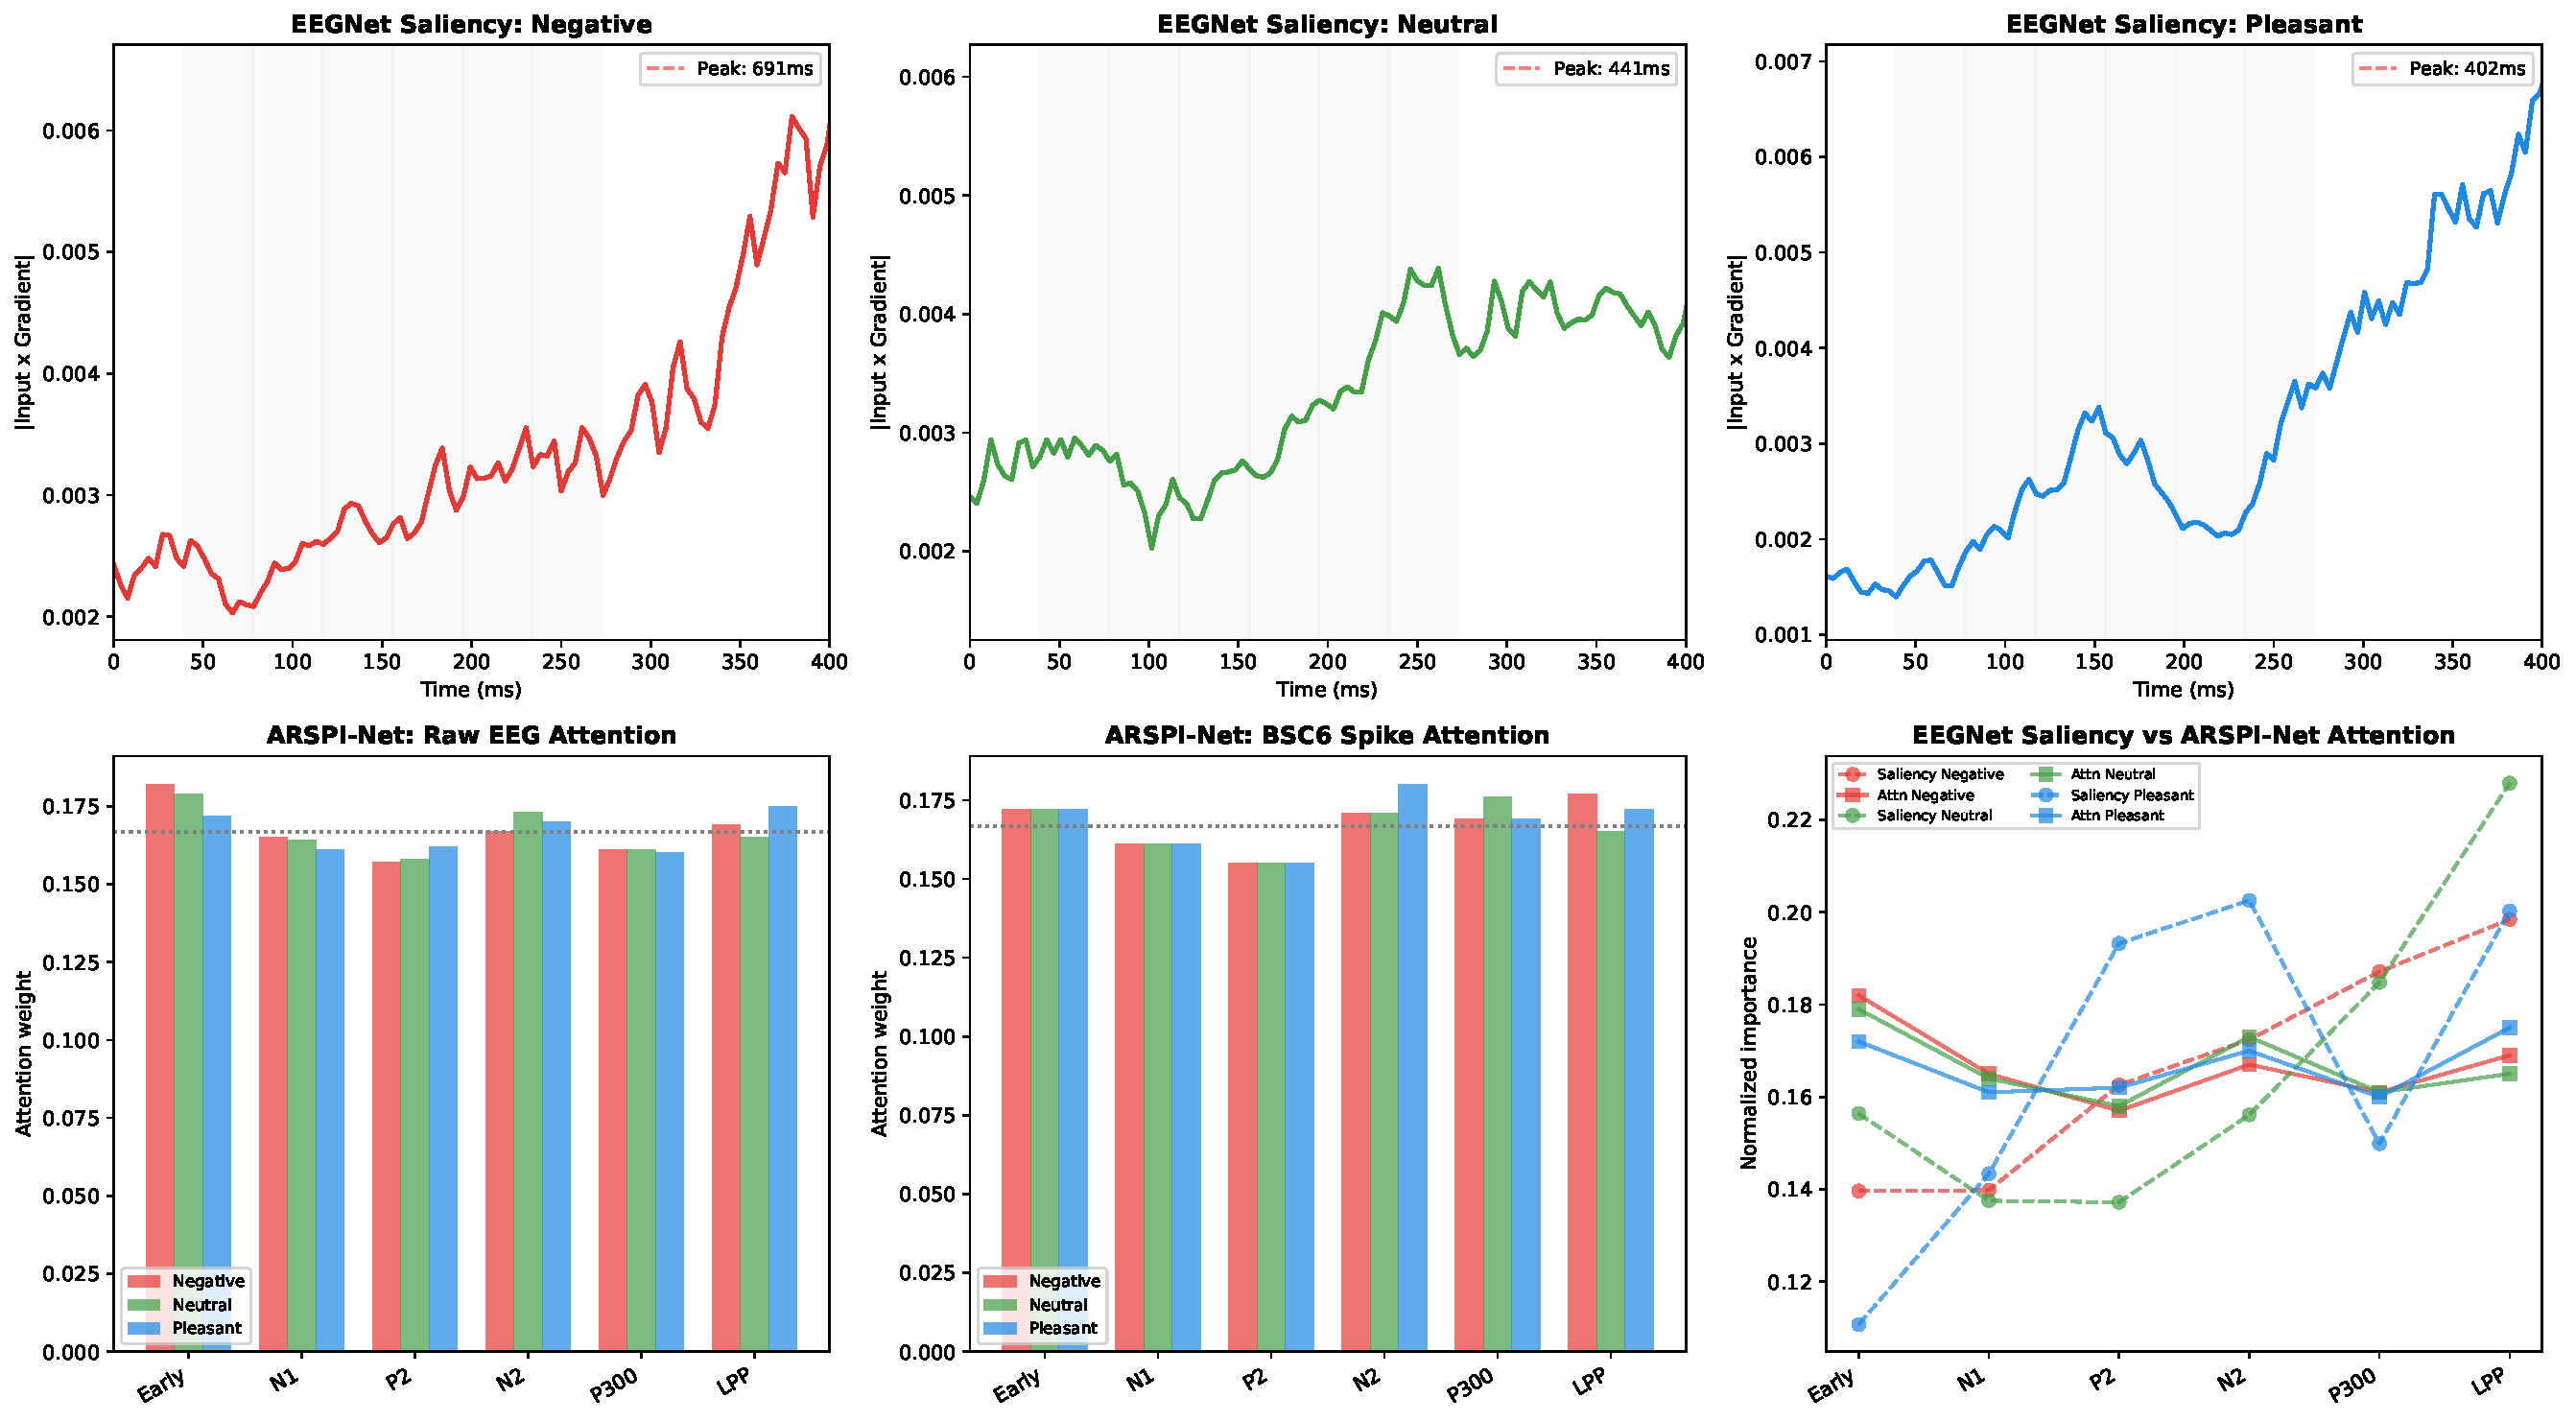
\includegraphics[width=\textwidth]{pictures/chGraphNeuralNetworks/fig_shap_comparison.pdf}
\caption{Temporal attribution comparison between EEGNet (Input$\times$Gradient saliency, top row) and ARSPI-Net (learned attention weights, bottom left/center). Top row: EEGNet saliency peaks at $691$~ms (Negative), $441$~ms (Neutral), $402$~ms (Pleasant)---all beyond the classical ERP window. Bottom right: when binned into BSC$_6$ temporal windows, EEGNet saliency shows monotonically increasing importance toward late bins (dashed), while ARSPI-Net attention shows condition-specific peaks within the ERP epoch (solid). EEGNet achieves $86.3\%$ accuracy but its temporal attribution does not align with classical ERP components; ARSPI-Net achieves lower accuracy but produces temporally interpretable, condition-differentiated explanations.}
\label{fig:shap_comparison}
\end{figure}

\paragraph{Interpretation.} This comparison illustrates the fundamental distinction between post-hoc and intrinsic interpretability. EEGNet's gradient saliency describes \emph{what the model learned to attend to}---late-epoch features that maximize classification accuracy. ARSPI-Net's attention describes \emph{what the signal contains}---condition-specific temporal structure within named ERP windows, produced by a fixed reservoir transformation whose dynamics are fully characterized. If EEGNet learned a shortcut (e.g., slow drift correlated with condition), the saliency faithfully explains the shortcut. ARSPI-Net's attention cannot exploit shortcuts because the reservoir weights are not trained---the temporal attention operates on features determined by the input signal and the known LIF dynamics, not by a learned function. The $10.4$~pp accuracy gap ($86.3\%$ vs.\ $57.5$--$66.7\%$) is the measured cost of this constraint, and it quantifies the accuracy--interpretability frontier for this signal class.




\section{Connection to Dynamical Analysis}
\label{sec:ch5_bridge}

This chapter characterized the discriminative embedding layer and spatial-topological layer of ARSPI-Net. The layer ablation (Section~\ref{sec:ch5_ablation}) demonstrated that the embedding dominates emotion classification while different clinical disorders are most detectable in different layers. The observation that the dynamical metrics (D block) carry the strongest SUD and PTSD clinical signals---outperforming the embedding on these specific detection tasks---raises a natural question: what are the dynamical properties of the reservoir's internal trajectory, and why do they encode clinical information that the classification embedding does not? Chapter~\ref{chap:dynamics} opens the reservoir and characterizes its driven trajectory as an independent source of interpretable descriptors. Chapter~\ref{chap:synthesis} then measures the coupling between the dynamical and topological layers across the electrode array.


\section{Chapter Summary}
\label{sec:ch5_summary}

This chapter makes eight contributions validated on $211$ subjects ($633$ observations at three-class; $844$ observations at four-class).

First, variance decomposition establishes that subject identity accounts for $62.6\%$ of embedding variance, with condition signal at $8.7\%$ ($7\times$ ratio). Subject-centering increases classification accuracy by $+13$ to $+21$~pp across all seven tested representations---including EEGNet ($72.0\% \to 89.1\%$), raw EEG ($70.5\% \to 88.4\%$), and ARSPI-Net ($59.4\% \to 78.8\%$)---confirming that subject-covariance entanglement is a signal-geometric property, not an artifact of any specific architecture.

Second, a Propagation Operating Characteristic across six graph densities, six propagation depths, three adjacency constructions, and four contrast-preserving operator families demonstrates that no graph operator exceeds the non-propagated baseline on this graph class.

Third, PCA nuisance regression monotonically destroys accuracy because subject and condition share principal components---a structural discovery about the geometry of multichannel affective EEG embeddings.

Fourth, graph-topological analysis reveals that Substance Use Disorder modulates emotional network reactivity across three complementary metrics ($p = 0.0004$, $0.003$, $0.012$), validated by permutation testing and internal replication.

Fifth, the paired-granularity comparison identifies a regime boundary: the reservoir outperforms band-power by $+12.5$~pp at three-class but is outperformed by $-6.2$~pp at four-class. The condition variance fraction drops from $8.7\%$ to $2.4\%$, and PTSD displaces SUD as the strongest clinical effect when within-valence resolution is available.

Sixth, the layer ablation matrix demonstrates that the embedding dominates emotion classification ($59.4\%$ vs.\ $42.2\%$ for dynamics, $35.3\%$ for topology), confirming that the reservoir's temporal coding carries the richest linearly separable condition signal.

Seventh, the clinical ablation reveals that different layers carry the strongest clinical sensitivity for different disorders---dynamics for SUD and PTSD, topology for GAD, coupling for ADHD---supporting the interpretation that ARSPI-Net's three response layers are operationally distinct and provide layer-specific clinical interpretability that no single-stage classifier can match.

Eighth, a comprehensive baseline comparison with centered evaluation establishes that the centering intervention dominates architecture choice: ARSPI-Net ($78.8\%$ centered) matches trained GRU ($78.4\%$) with zero trainable recurrent parameters, while providing a fully traceable, intrinsically interpretable signal chain from input ERP to classification output.